\documentclass[a4paper]{article}

\def\npart {III}
\def\nterm {Lent}
\def\nyear {2017}
\def\nlecturer {D.\ B.\ Skinner}
\def\ncourse {Advanced Quantum Field Theory}

% Imports
\ifx \nextra \undefined
  \usepackage[pdftex,
    hidelinks,
    pdfauthor={Dexter Chua},
    pdfsubject={Cambridge Maths Notes: Part \npart\ - \ncourse},
    pdftitle={Part \npart\ - \ncourse},
  pdfkeywords={Cambridge Mathematics Maths Math \npart\ \nterm\ \nyear\ \ncourse}]{hyperref}
  \title{Part \npart\ - \ncourse}
\else
  \usepackage[pdftex,
    hidelinks,
    pdfauthor={Dexter Chua},
    pdfsubject={Cambridge Maths Notes: Part \npart\ - \ncourse\ (\nextra)},
    pdftitle={Part \npart\ - \ncourse\ (\nextra)},
  pdfkeywords={Cambridge Mathematics Maths Math \npart\ \nterm\ \nyear\ \ncourse\ \nextra}]{hyperref}

  \title{Part \npart\ - \ncourse \\ {\Large \nextra}}
\fi

\author{Lectured by \nlecturer \\\small Notes taken by Dexter Chua}
\date{\nterm\ \nyear}

\usepackage{alltt}
\usepackage{amsfonts}
\usepackage{amsmath}
\usepackage{amssymb}
\usepackage{amsthm}
\usepackage{booktabs}
\usepackage{caption}
\usepackage{enumitem}
\usepackage{fancyhdr}
\usepackage{graphicx}
\usepackage{mathtools}
\usepackage{microtype}
\usepackage{multirow}
\usepackage{pdflscape}
\usepackage{pgfplots}
\usepackage{siunitx}
\usepackage{tabularx}
\usepackage{tikz}
\usepackage{tkz-euclide}
\usepackage[normalem]{ulem}
\usepackage[all]{xy}

\pgfplotsset{compat=1.12}

\pagestyle{fancyplain}
\lhead{\emph{\nouppercase{\leftmark}}}
\ifx \nextra \undefined
  \rhead{
    \ifnum\thepage=1
    \else
      \npart\ \ncourse
    \fi}
\else
  \rhead{
    \ifnum\thepage=1
    \else
      \npart\ \ncourse\ (\nextra)
    \fi}
\fi
\usetikzlibrary{arrows}
\usetikzlibrary{decorations.markings}
\usetikzlibrary{decorations.pathmorphing}
\usetikzlibrary{positioning}
\usetikzlibrary{fadings}
\usetikzlibrary{intersections}
\usetikzlibrary{cd}

\newcommand*{\Cdot}{\raisebox{-0.25ex}{\scalebox{1.5}{$\cdot$}}}
\newcommand {\pd}[2][ ]{
  \ifx #1 { }
    \frac{\partial}{\partial #2}
  \else
    \frac{\partial^{#1}}{\partial #2^{#1}}
  \fi
}

% Theorems
\theoremstyle{definition}
\newtheorem*{aim}{Aim}
\newtheorem*{axiom}{Axiom}
\newtheorem*{claim}{Claim}
\newtheorem*{cor}{Corollary}
\newtheorem*{defi}{Definition}
\newtheorem*{eg}{Example}
\newtheorem*{fact}{Fact}
\newtheorem*{law}{Law}
\newtheorem*{lemma}{Lemma}
\newtheorem*{notation}{Notation}
\newtheorem*{prop}{Proposition}
\newtheorem*{thm}{Theorem}

\renewcommand{\labelitemi}{--}
\renewcommand{\labelitemii}{$\circ$}
\renewcommand{\labelenumi}{(\roman{*})}

\let\stdsection\section
\renewcommand\section{\newpage\stdsection}

% Strike through
\def\st{\bgroup \ULdepth=-.55ex \ULset}

% Maths symbols
\newcommand{\bra}{\langle}
\newcommand{\ket}{\rangle}

\newcommand{\N}{\mathbb{N}}
\newcommand{\Z}{\mathbb{Z}}
\newcommand{\Q}{\mathbb{Q}}
\renewcommand{\H}{\mathbb{H}}
\newcommand{\R}{\mathbb{R}}
\newcommand{\C}{\mathbb{C}}
\newcommand{\Prob}{\mathbb{P}}
\renewcommand{\P}{\mathbb{P}}
\newcommand{\E}{\mathbb{E}}
\newcommand{\F}{\mathbb{F}}
\newcommand{\cU}{\mathcal{U}}
\newcommand{\RP}{\mathbb{RP}}
\newcommand{\CP}{\mathbb{CP}}

\newcommand{\ph}{\,\cdot\,}

\DeclareMathOperator{\sech}{sech}
\DeclareMathOperator{\cosech}{cosech}
\DeclareMathOperator{\cosec}{cosec}

\DeclareMathOperator{\covol}{covol}
\DeclareMathOperator{\vol}{vol}

\let\Im\relax
\let\Re\relax
\DeclareMathOperator{\Im}{Im}
\DeclareMathOperator{\Re}{Re}
\DeclareMathOperator{\im}{im}
\DeclareMathOperator{\image}{image}
\DeclareMathOperator{\Ann}{Ann}

\DeclareMathOperator*{\res}{res}
\DeclareMathOperator{\Res}{Res}
\DeclareMathOperator{\Ind}{Ind}

\DeclareMathOperator{\tr}{tr}
\DeclareMathOperator{\diag}{diag}
\DeclareMathOperator{\rank}{rank}
\DeclareMathOperator{\card}{card}
\DeclareMathOperator{\spn}{span}
\DeclareMathOperator{\adj}{adj}

\DeclareMathOperator{\erf}{erf}
\DeclareMathOperator{\erfc}{erfc}

\DeclareMathOperator{\ord}{ord}
\DeclareMathOperator{\Sym}{Sym}

\DeclareMathOperator{\sgn}{sgn}
\DeclareMathOperator{\orb}{orb}
\DeclareMathOperator{\stab}{stab}
\DeclareMathOperator{\ccl}{ccl}

\DeclareMathOperator{\lcm}{lcm}
\DeclareMathOperator{\hcf}{hcf}

\DeclareMathOperator{\Int}{Int}
\DeclareMathOperator{\id}{id}

\DeclareMathOperator{\betaD}{beta}
\DeclareMathOperator{\gammaD}{gamma}
\DeclareMathOperator{\Poisson}{Poisson}
\DeclareMathOperator{\binomial}{binomial}
\DeclareMathOperator{\multinomial}{multinomial}
\DeclareMathOperator{\Bernoulli}{Bernoulli}
\DeclareMathOperator{\like}{like}

\DeclareMathOperator{\var}{var}
\DeclareMathOperator{\cov}{cov}
\DeclareMathOperator{\bias}{bias}
\DeclareMathOperator{\mse}{mse}
\DeclareMathOperator{\corr}{corr}

\DeclareMathOperator{\otp}{otp}
\DeclareMathOperator{\dom}{dom}

\DeclareMathOperator{\Root}{Root}
\DeclareMathOperator{\supp}{supp}
\DeclareMathOperator{\rel}{rel}
\DeclareMathOperator{\Hom}{Hom}
\DeclareMathOperator{\Aut}{Aut}
\DeclareMathOperator{\Gal}{Gal}
\DeclareMathOperator{\Mat}{Mat}
\DeclareMathOperator{\End}{End}
\DeclareMathOperator{\Char}{char}
\DeclareMathOperator{\ev}{ev}
\DeclareMathOperator{\St}{St}
\DeclareMathOperator{\Lk}{Lk}
\DeclareMathOperator{\disc}{disc}
\DeclareMathOperator{\Isom}{Isom}
\DeclareMathOperator{\length}{length}
\DeclareMathOperator{\energy}{energy}
\DeclareMathOperator{\area}{area}
\DeclareMathOperator{\Syl}{Syl}
\DeclareMathOperator{\cl}{cl}
\DeclareMathOperator{\fix}{fix}

\newcommand{\GL}{\mathrm{GL}}
\newcommand{\SL}{\mathrm{SL}}
\newcommand{\PGL}{\mathrm{PGL}}
\newcommand{\PSL}{\mathrm{PSL}}
\newcommand{\PSU}{\mathrm{PSU}}
\newcommand{\Or}{\mathrm{O}}
\newcommand{\SO}{\mathrm{SO}}
\newcommand{\U}{\mathrm{U}}
\newcommand{\SU}{\mathrm{SU}}

\renewcommand{\d}{\mathrm{d}}
\newcommand{\D}{\mathrm{D}}

\tikzset{->/.style = {decoration={markings,
                                  mark=at position 1 with {\arrow[scale=2]{latex'}}},
                      postaction={decorate}}}
\tikzset{<-/.style = {decoration={markings,
                                  mark=at position 0 with {\arrowreversed[scale=2]{latex'}}},
                      postaction={decorate}}}
\tikzset{<->/.style = {decoration={markings,
                                   mark=at position 0 with {\arrowreversed[scale=2]{latex'}},
                                   mark=at position 1 with {\arrow[scale=2]{latex'}}},
                       postaction={decorate}}}
\tikzset{->-/.style = {decoration={markings,
                                   mark=at position #1 with {\arrow[scale=2]{latex'}}},
                       postaction={decorate}}}
\tikzset{-<-/.style = {decoration={markings,
                                   mark=at position #1 with {\arrowreversed[scale=2]{latex'}}},
                       postaction={decorate}}}

\tikzset{circ/.style = {fill, circle, inner sep = 0, minimum size = 3}}
\tikzset{mstate/.style={circle, draw, blue, text=black, minimum width=0.7cm}}

\definecolor{mblue}{rgb}{0.2, 0.3, 0.8}
\definecolor{morange}{rgb}{1, 0.5, 0}
\definecolor{mgreen}{rgb}{0.1, 0.4, 0.2}
\definecolor{mred}{rgb}{0.5, 0, 0}

\def\drawcirculararc(#1,#2)(#3,#4)(#5,#6){%
    \pgfmathsetmacro\cA{(#1*#1+#2*#2-#3*#3-#4*#4)/2}%
    \pgfmathsetmacro\cB{(#1*#1+#2*#2-#5*#5-#6*#6)/2}%
    \pgfmathsetmacro\cy{(\cB*(#1-#3)-\cA*(#1-#5))/%
                        ((#2-#6)*(#1-#3)-(#2-#4)*(#1-#5))}%
    \pgfmathsetmacro\cx{(\cA-\cy*(#2-#4))/(#1-#3)}%
    \pgfmathsetmacro\cr{sqrt((#1-\cx)*(#1-\cx)+(#2-\cy)*(#2-\cy))}%
    \pgfmathsetmacro\cA{atan2(#2-\cy,#1-\cx)}%
    \pgfmathsetmacro\cB{atan2(#6-\cy,#5-\cx)}%
    \pgfmathparse{\cB<\cA}%
    \ifnum\pgfmathresult=1
        \pgfmathsetmacro\cB{\cB+360}%
    \fi
    \draw (#1,#2) arc (\cA:\cB:\cr);%
}
\newcommand\getCoord[3]{\newdimen{#1}\newdimen{#2}\pgfextractx{#1}{\pgfpointanchor{#3}{center}}\pgfextracty{#2}{\pgfpointanchor{#3}{center}}}

\def\Xint#1{\mathchoice
   {\XXint\displaystyle\textstyle{#1}}%
   {\XXint\textstyle\scriptstyle{#1}}%
   {\XXint\scriptstyle\scriptscriptstyle{#1}}%
   {\XXint\scriptscriptstyle\scriptscriptstyle{#1}}%
   \!\int}
\def\XXint#1#2#3{{\setbox0=\hbox{$#1{#2#3}{\int}$}
     \vcenter{\hbox{$#2#3$}}\kern-.5\wd0}}
\def\ddashint{\Xint=}
\def\dashint{\Xint-}


\makeatletter
\newcommand*{\textoverline}[1]{$\overline{\hbox{#1}}\m@th$}
\makeatother
\usepackage[compat=1.1.0]{tikz-feynman}
\tikzfeynmanset{/tikzfeynman/momentum/arrow shorten = 0.3}
\tikzfeynmanset{/tikzfeynman/warn luatex = false}

\usepackage{pgfplots}

\DeclareRobustCommand{\ghost}{\tikz[baseline=.1em,scale=.5]{
  \draw [fill=yellow] (0, 0) -- (0, 0.45) arc (+180:0:0.3) -- (0.6, 0);
  \draw [decorate, decoration={snake, amplitude=0.7, segment length=2.3}] (0.6, 0) -- (0, 0);
  \fill[black] (0.18, 0.45) circle [radius=0.05];
  \fill[black] (0.44, 0.45) circle [radius=0.05];
}}

\begin{document}
\maketitle
{\small
\setlength{\parindent}{0em}
\setlength{\parskip}{1em}

Quantum Field Theory (QFT) provides the most profound description of Nature we currently possess. As well as being the basic theoretical framework for describing elementary particles and their interactions (excluding gravity), QFT also plays a major role in areas of physics and mathematics as diverse as string theory, condensed matter physics, topology and geometry, astrophysics and cosmology.

This course builds on the Michaelmas Quantum Field Theory course, using techniques of path integrals and functional methods to study quantum gauge theories. Gauge Theories are a generalisation of electrodynamics and form the backbone of the Standard Model --- our best theory encompassing all particle physics. In a gauge theory, fields have an infinitely redundant description; we can transform the fields by a different element of a Lie Group at every point in space-time and yet still describe the same physics. Quantising a gauge theory requires us to eliminate this infinite redundancy. In the path integral approach, this is done using tools such as ghost fields and BRST symmetry. We discuss the construction of gauge theories and their most important observables, Wilson Loops. Time permitting, we will explore the possibility that a classical symmetry may be broken by quantum effects. Such anomalies have many important consequences, from constraints on interactions between matter and gauge fields, to the ability to actually render a QFT inconsistent.

A further major component of the course is to study Renormalization. Wilson's picture of Renormalisation is one of the deepest insights into QFT --- it explains why we can do physics at all! The essential point is that the physics we see depends on the scale at which we look. In QFT, this dependence is governed by evolution along the Renormalisation Group (RG) flow. The course explores renormalisation systematically, from the use of dimensional regularisation in perturbative loop integrals, to the difficulties inherent in trying to construct a quantum field theory of gravity. We discuss the various possible behaviours of a QFT under RG flow, showing in particular that the coupling constant of a non-Abelian gauge theory can effectively become small at high energies. Known as "asymptotic freedom", this phenomenon revolutionised our understanding of the strong interactions. We introduce the notion of an Effective Field Theory that describes the low energy limit of a more fundamental theory and helps parametrise possible departures from this low energy approximation. From a modern perspective, the Standard Model itself appears to be but an effective field theory.

\subsubsection*{Pre-requisites}
Knowledge of the Michaelmas term Quantum Field Theory course will be assumed. Familiarity with the course Symmetries, Fields and Particles would be very helpful.
}
\tableofcontents

\setcounter{section}{-1}
\section{Introduction}
\subsection{What is quantum field theory}
What is Quantum Field Theory? The first answer we might give is --- it's just a quantum version of a field theory (duh!). We know the world is described by fields, e.g.\ electromagnetic fields, and the world is quantum. So naturally we want to find a quantum version of field theory. Indeed, this is what drove the study of quantum field theory historically.

But there are other things we can use quantum field theory for, and they are not so obviously fields. In a lot of condensed matter applications, we can use quantum field theory techniques to study, say, vibrations of a crystal, and its quanta are known as ``phonons''. More generally, we can use quantum field theory to study things like phase transitions (e.g.\ boiling water). This is not so obvious a place you think quantum field theory will happen, but it is. Some people even use quantum field theory techniques to study the spread of diseases in a population!

We can also use quantum field theory to study problems in mathematics! QFT is used to study knot invariants, which are ways to assign labels to different types of knots to figure out if they are the same. Donaldson won a fields medal for showing that there are inequivalent differentiable structures on $\R^4$, and this used techniques coming from quantum Yang--Mills theory as well.

These are not things we would traditionally think of as quantum field theory. In this course, we are not going to be calculating, say, Higgs corrections to $\gamma\gamma$-interactions. Instead, we try to understand better this machinery known as quantum field theory.

\subsection{Building a quantum field theory}
We now try to give a very brief outline of how one does quantum field theory. Roughly, we follow the steps below:
\begin{enumerate}
  \item We pick a space to represent our ``universe''. This will always be a manifold, but we usually impose additional structure on it.
    \begin{itemize}
      \item In particle physics, we often pick the manifold to be a $4$-dimensional pseudo-Riemannian manifold of signature $+---$. Usually, we in fact pick $(M, g) = (\R^4, \eta)$ where $\eta$ is the usual Minkowski metric.
      \item In condensed matter physics, we often choose $(M, g) = (\R^3, \delta)$, where $\delta$ is the flat Euclidean metric.
      \item In string theory, we have fields living on Riemann surface $\Sigma$ (e.g.\ sphere, torus). Instead of specifying a metric, we only specify the conformal equivalence class $[g]$ of the metric, i.e.\ the metric up to a scalar factor.
      \item In QFT for knots, we pick $M$ to be some oriented $3$-manifold, e.g.\ $S^3$, but with \emph{no} metric.
      \item In this course, we will usually take $(M, g) = (\R^d, \delta)$ for some $d$, where $\delta$ is again the flat, Euclidean metric.

        We might think this is a very sensible and easy choice, because we are all used to working in $(\R^d, \delta)$. However, mathematically, this space is non-compact, and it will lead to a lot of annoying things happening.
    \end{itemize}
  \item We pick some fields. The simplest choice is just a function $\phi: M \to \R$ or $\C$. This is a \term{scalar field}. Slightly more generally, we can also have $\phi: M \to N$ for some other manifold $N$. We call $N$ the \term{target space}.

    For example, quantum mechanics is a quantum field theory. Here we choose $M$ to be some interval $M = I = [0, 1]$, which we think of as time, and the field is a map $\phi: I \to \R^3$. We think of this as a path in $\R^3$.
    \begin{center}
      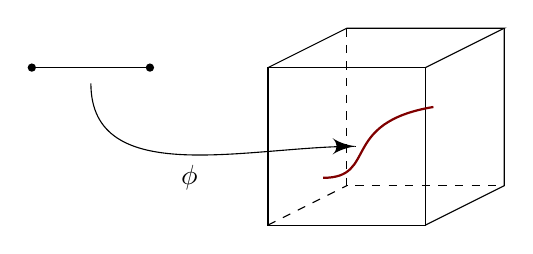
\begin{tikzpicture}
        \draw (0, 0) node [circ] {} -- (1.5, 0) node [circ] {};

        \draw (3, 0) rectangle (5, -2);
        \draw (3, 0) -- (4, 0.5) -- (6, 0.5) -- (5, 0);
        \draw (6, 0.5) -- (6, -1.5) -- (5, -2);
        \draw [dashed] (4, 0.5) -- (4, -1.5) -- (6, -1.5);
        \draw [dashed] (3, -2) -- (4, -1.5);

        \draw (0.75, -0.2) edge [out=270, in=180] (4.1, -1);

        \node at (2, -1.4) {$\phi$};

        \draw [->] (4.099, -1) -- (4.1, -1);

        \draw [thick, mred](3.7, -1.4) .. controls (4.4, -1.4) and (3.9, -0.7) .. (5.1, -0.5);
      \end{tikzpicture}
    \end{center}
    In string theory, we often have fields $\phi: \Sigma \to N$, where $N$ is a \emph{Calabi--Yau manifold}.

    In pion physics, $\pi(x)$ describes a map $\phi: (\R^4, \eta) \to G/H$, where $G$ and $H$ are Lie groups.

    Of course, we can go beyond scalar fields. We can also have fields with non-zero spin such as fermions or gauge fields, e.g.\ a connection on a principal $G$-bundle, as we will figure out later. These are fields that carry a non-trivial representation of the Lorentz group. There is a whole load of things we can choose for our field.

    Whatever field we choose, we let $\mathcal{C}$\index{$\mathcal{C}$} be the space of all field configurations, i.e.\ a point $\phi \in \mathcal{C}$ represents a picture of our field across all of $M$. Thus $\mathcal{C}$ is some form of function space and will typically be infinite dimensional. This infinite-dimensionality is what makes QFT hard, and also what makes it interesting.

  \item We choose an action. An \emph{action} is just a function $S: \mathcal{C} \to \R$. You tell me what the field looks like, and I will give you a number, the value of the action. We often choose our action to be local, in the sense that we assume there exists some function $\mathcal{L}(\phi, \partial \phi, \cdots)$ such that
    \[
      S[\phi] = \int_M\d^4 x \sqrt{g}\; \mathcal{L}(\phi(x), \partial\phi (x), \cdots).
    \]
    The physics motivation behind this choice is obvious --- we don't want what is happening over here to depend on what is happening at the far side of Pluto. However, this assumption is actually rather suspicious, and we will revisit this later.

    For example, we have certainly met actions that look like
    \[
      S[\phi] = \int \d^4 x\; \left(\frac{1}{2} (\partial \phi)^2 + \frac{m^2}{2} \phi^2 + \frac{\lambda}{4!} \phi^4\right),
    \]
    and for gauge fields we might have seen
    \[
      S[A] = \frac{1}{4} \int \d^4 x\; F_{\mu\nu}F^{\mu\nu}.
    \]
    If we have a coupled fermion field, we might have
    \[
      S[A, \psi] = \frac{1}{4} \int \d^4 x\; F_{\mu\nu}F^{\mu\nu} + \bar\psi (\slashed{D} + m) \psi.
    \]
    But recall when we first encountered Lagrangians in classical dynamics, we worked with \emph{lots} of different Lagrangians. We can do whatever thing we like, make the particle roll down the hill and jump into space etc, and we get to deal with a whole family of different Lagrangians. But when we come to quantum field theory, the choices seem to be rather restrictive. Why can't we choose something like
    \[
      S[A] = \int F^2 + F^4 + \cosh(F^2) + \cdots?
    \]
    It turns out we can, and in fact we \emph{must}. We will have to work with something much more complicated.

    But then what were we doing in the QFT course? Did we just waste time coming up with tools that just work with these very specific examples? It turns out not. We will see that there are very good reasons to study these specific actions.
  \item What do we compute? In this course, the main object we'll study is the \term{partition function}
    \[
      \mathcal{Z} = \int_\mathcal{C} \D \phi\; e^{-S[\phi]/\hbar},
    \]
    which is some sort of integral over the space of all fields. Note that the minus sign in the exponential is for the Euclidean signature. If we are not Euclidean, we get some $i$'s instead.

    We will see that the factor of $e^{-S[\phi]/\hbar}$ means that as $\hbar \to 0$, the dominant contribution to the partition function comes from stationary points of $S[\phi]$ over $\mathcal{C}$, and this starts to bring us back to the classical theory of fields. The effect of $e^{-S[\phi]/\hbar}$ is to try to suppress ``wild'' contributions to $\mathcal{Z}$, e.g.\ where $\phi$ is varying very rapidly or $\phi$ takes very large values.

     Heuristically, just as in statistical physics, we have a competition between the two factors $\D \phi$ and $e^{-S[\phi]/\hbar}$. The action part tries to suppress crazy things, but how well this happens depends on how much crazy things are happening, which is measured by the measure $\D \phi$. We can think of this $\D \phi$ as ``entropy''.

     However, the problem is, the measure $\D \phi$ on $\mathcal{C}$ doesn't actually exist! Understanding what we mean by this path integral, and what this measure actually is, and how we can actually compute this thing, and how this has got to do with the canonical quantization operators we had previously, is the main focus of the first part of this course.
\end{enumerate}

\section{QFT in zero dimensions}
We start from the simplest case we can think of, namely quantum field theory in zero dimensions. This might seem like an absurd thing to study --- the universe is far from being zero-dimensional. However, it turns out this is the case where we can make sense of the theory mathematically. Thus, it is important to study 0-dimensional field theories and understand what is going on.

There are two reasons for this. As mentioned, we cannot actually define the path integral in higher dimensions. Thus, if we were to do this ``properly'', we will have to define it as the limit of something that is effectively a zero-dimensional quantum field theory. The other reason is that in this course, we are not going to study higher-dimensional path integrals ``rigorously''. What we are going to do is that we will study zero-dimensional field theories rigorously, and then assume that analogous results hold for higher-dimensional field theories.

One drawback of this approach is that what we do in this section will have little physical content or motivation. We will just assume that the partition function is something we are interested about, without actually relating it to any physical processes. In the next chapter, on one-dimensional field theories, we are going see why this is an interesting thing to study.

Let's begin. In $d = 0$, if our universe $M$ is connected, then the only choice of $M$ is $\{\mathrm{pt}\}$. There is a no possibility for a field to have spin, because the Lorentz group is trivial. Our fields are scalar, and the simplest choice is just a single field $\phi: \{\mathrm{pt}\} \to \R$, i.e.\ just a real variable. Similarly, we simply have $\mathcal{C} \cong \R$. This is \emph{not} an infinite-dimensional space.

The action is just a normal function $S: \mathcal{C} \cong \R \to \R$ of one real variable. The path integral measure $\D \phi$ can be taken to just be the standard (Lebesgue) measure $\d \phi$ on $\R$. So our partition function is just
\[
  \mathcal{Z} = \int_\R \d \phi\; e^{-S(\phi)/\hbar},
\]
where we assume $S$ is chosen so that this converges. This happens if $S$ grows sufficiently large as $\phi \to \pm \infty$.

More generally, we may wish to compute \term{correlation functions}, i.e.\ we pick another function $f(\phi)$ and compute the \term{expectation}\index{$\bra f(\phi)\ket$}
\[
  \bra f(\phi)\ket = \frac{1}{\mathcal{Z}} \int \d \phi\; f(\phi) e^{-S(\phi)/\hbar}.
\]
Again, we can pick whatever $f$ we like as long as the integral converges. In this case, $\frac{1}{\mathcal{Z}} e^{-S(\phi)/\hbar}$ is a probability distribution on $\R$, and as the name suggests, $\bra f(\phi)\ket$ is just the expectation value of $f$ in this distribution. Later on, when we study quantum field theory in higher dimensions, we can define more complicated $f$ by evaluating $\phi$ at different points, and we can use this to figure out how the field at different points relate to each other.

Our action is taken to have a series expansion in $\phi$, so in particular we can write
\[
  S(\phi) = \frac{m^2 \phi^2}{2} + \sum_{n = 3}^N g_n \frac{\phi^n}{n!}.
\]
We didn't put in a constant term, as it would just give us a constant factor in $\mathcal{Z}$. We could have included linear terms, but we shall not. The important thing is that $N$ has to be even, so that the asymptotic behaviour of $S$ is symmetric in both sides.

Now the partition function is a function of all these terms: $\mathcal{Z} = \mathcal{Z}(m^2, g_n)$. Similarly, $\bra f\ket$ is again a function of $m^2$ and $g_n$, and possibly other things used to define $f$ itself.

Note that \emph{nothing} depends on the field, because we are integrating over all possible fields.

\subsection{Free theories}
We consider the simplest possible QFT. These QFT's are free, and so $S(\phi)$ is at most quadratic. Classically, this implies the equations of motions are linear, and so there is superposition, and thus the particles do not interact.

Let $\phi: \{\mathrm{pt}\} \to \R^n$ be a field with coordinates $\phi^a$, and define
\[
  S(\phi) = \frac{1}{2} M(\phi, \phi) = \frac{1}{2} M_{ab} \phi^a \phi^b,
\]
where $M: \R^n \times \R^n \to \R$ is a positive-definite symmetric matrix. Then the partition function $\mathcal{Z}(M)$ is just a Gaussian integral:
\[
  \mathcal{Z}(M) = \int_{\R^n} \d^n \phi\; e^{- \frac{1}{2\hbar} M(\phi, \phi)} = \frac{(2 \pi \hbar)^{n/2}}{\sqrt{\det{M}}}.
\]
Indeed, to compute this integral, since $M$ is symmetric, there exists an orthogonal transformation $O: \R^n \to \R^n$ that diagonalizes it. The measure $\d^n \phi$ is invariant under orthogonal transformations. So in terms of the eigenvectors of $M$, this just reduces to a product of $n$ 1D Gaussian integrals of this type, and this is a standard integral:
\[
  \int \d \chi\; e^{-m\chi^2/2\hbar} = \sqrt{\frac{2\pi \hbar}{m}}.
\]
In our case, $m > 0$ runs over all eigenvalues of $M$, and the product of eigenvalues is exactly $\det M$.

A small generalization is useful. We let
\[
  S(\phi) = \frac{1}{2} M(\phi, \phi) + J(\phi),
\]
where $J: \R^n \to \R$ is some linear map (we can think of $J$ as a (co)vector, and also write $J(\phi) = J \cdot \phi$). $J$ is a \emph{source} in the classical case. Then in this theory, we have
\[
  \mathcal{Z}(M, J) = \int_{\R^n} \d^n \phi\; \exp\left(-\frac{1}{\hbar}\left(\frac{1}{2} M(\phi, \phi) + J(\phi)\right)\right).
\]
To do this integral, we complete the square by letting $\tilde{\phi} = \phi + M^{-1}J$. In other words,
\[
  \tilde{\phi}^a = \phi^a + (M^{-1})^{ab} J_b.
\]
The inverse exists because $M$ is assumed to be positive definite. We can now complete the square to find
\begin{align*}
  \mathcal{Z}(M, J) &= \int_{\R^n} \d^n \tilde{\phi} \;\exp\left(\frac{-1}{2\hbar}M(\tilde{\phi}, \tilde{\phi}) + \frac{1}{2\hbar}M^{-1}(J, J)\right)\\
  &= \exp\left(\frac{1}{2\hbar}M^{-1}(J, J)\right)\int_{\R^n} \d^n \tilde{\phi} \;\exp\left(\frac{-1}{2\hbar}M(\tilde{\phi}, \tilde{\phi})\right)\\
  &= \exp\left(\frac{1}{2\hbar}M^{-1}(J, J)\right) \frac{(2\pi \hbar)^{n/2}}{\sqrt{\det M}}.
\end{align*}
In the long run, we really don't care about the case with a source. However, we will use this general case to compute some correlation functions.

We return to the case without a source, and let $P: \R^n \to \R$ be a polynomial. We want to compute
\[
  \bra P(\phi)\ket = \frac{1}{\mathcal{Z}(M)} \int_{\R^n} \d^n \phi\; P(\phi) \exp\left(-\frac{1}{2\hbar} M(\phi, \phi)\right).
\]
By linearity, it suffices to consider the case where $P$ is just a monomial, so
\[
  P(\phi) = \prod_{i = 1}^m (\ell_i(\phi)),
\]
for $\ell_i : \R^n \to \R$ linear maps. Now if $m$ is odd, then clearly $\bra P(\phi)\ket = 0$, since this is an integral of an odd function. When $m = 2k$, then we have
\[
  \bra P(\phi) \ket = \frac{1}{\mathcal{Z}(M)} \int \d^n \phi\; (\ell_i\cdot \phi) \cdots (\ell_{2k} \cdot \phi) \exp\left(-\frac{1}{2\hbar}M (\phi, \phi) - \frac{J \cdot \phi}{\hbar}\right).
\]
Here we are eventually going to set $J = 0$, but for the time being, we will be silly and put the source there. The relevance is that we can then think of our factors $\ell_i \cdot \phi$ as derivatives with respect to $J$:
\begin{align*}
  \bra P(\phi)\ket &= \frac{(-\hbar)^{2k}}{\mathcal{Z}(M)} \int \d^n \phi \; \prod_{i = 1}^{2k} \left(\ell_i \cdot \frac{\partial}{\partial J}\right) \exp\left(-\frac{1}{2\hbar} M(\phi, \phi) - \frac{J\cdot \phi}{\hbar}\right)\\
  \intertext{Since the integral is absolutely convergent, we can move the derivative out of the integral, and get}
  &= \frac{(-\hbar)^{2k}}{\mathcal{Z}(M)} \prod_{i = 1}^{2k} \left(\ell_i \cdot \frac{\partial}{\partial J}\right) \int \d^n \phi \; \exp\left(-\frac{1}{2\hbar} M(\phi, \phi) - \frac{J\cdot \phi}{\hbar}\right)\\
  &= \hbar^{2k} \prod_{i = 1}^{2k} \left(\ell_i \cdot \frac{\partial}{\partial J}\right) \exp\left(\frac{1}{2\hbar}M^{-1}(J, J)\right).
\end{align*}
When each derivative $\ell_i \cdot \frac{\partial}{\partial J}$ acts on the exponential, we obtain a factor of
\[
  \frac{1}{\hbar} M^{-1}(J, \ell_i).
\]
in front. At the end, we are going to set $J = 0$. So we only get contributions if and only if exactly half (i.e.\ $k$) of the derivatives act on the exponential, and the other $k$ act on the factor in front to get rid of the $J$.

We let $\sigma$ denote a (complete) pairing of the set $\{1, \cdots, 2k\}$, and $\Pi_{2k}$ be the set of all such pairings. For example, if we have $k = 2$, then the possible pairings are $\{(1, 2), (3, 4)\}$, $\{(1, 3), (2, 4)\}$ and $\{(1, 4), (2, 3)\}$:
\begin{center}
  \begin{tikzpicture}
    \node [circ] at (0, 0) {};
    \node [circ] at (1, 0) {};
    \node [circ] at (1, 1) {};
    \node [circ] at (0, 1) {};
    \draw (0, 0) -- (0, 1);
    \draw (1, 0) -- (1, 1);

    \begin{scope}[shift={(3, 0)}]
      \node [circ] at (0, 0) {};
      \node [circ] at (1, 0) {};
      \node [circ] at (1, 1) {};
      \node [circ] at (0, 1) {};
      \draw (0, 0) -- (1, 0);
      \draw (0, 1) -- (1, 1);
    \end{scope}

    \begin{scope}[shift={(6, 0)}]
      \node [circ] at (0, 0) {};
      \node [circ] at (1, 0) {};
      \node [circ] at (1, 1) {};
      \node [circ] at (0, 1) {};
      \draw (0, 0) -- (1, 1);
      \draw (1, 0) -- (0, 1);
    \end{scope}
  \end{tikzpicture}
\end{center}
In general, we have
\[
  |\Pi_{2k}| = \frac{(2k)!}{2^k k!},
\]
and we have
\begin{thm}[Wick's theorem]\index{Wick's theorem}
  For a monomial
  \[
    P(\phi) = \prod_{i = 1}^{2k} \ell_i(\phi),
  \]
  we have
  \[
    \bra P(\phi)\ket = \hbar^{k}\sum_{\sigma \in \Pi_{2k}} \prod_{i \in \{1, \cdots, 2k\}/\sigma} M^{-1}(\ell_i, \ell_{\sigma(i)}).
  \]
  where the $\{1, \cdots, 2k\}/\sigma$ says we sum over each pair $\{i, \sigma(i)\}$ only once, rather than once for $(i, \sigma(i))$ and another for $(\sigma(i), i)$.
\end{thm}
This is in fact the version of Wick's theorem for this 0d QFT, and $M^{-1}$ plays the role of the propagator.

For example, we have
\[
  \bra \ell_1(\phi) \ell_2(\phi)\ket = \hbar M^{-1} (\ell_1, \ell_2).
\]
We can represent this by the diagram
\begin{center}
  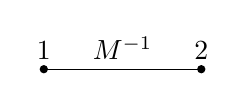
\begin{tikzpicture}
    \node [circ] at (0, 0) {};
    \node [circ] at (2, 0) {};

    \node [above] at (0, 0) {$1$};
    \node [above] at (2, 0) {$2$};
    \draw (0, 0) -- (2, 0) node [pos=0.5, above] {$M^{-1}$};
  \end{tikzpicture}
\end{center}
Similarly, we have
\begin{multline*}
  \bra \ell_1(\phi) \cdots \ell_4(\phi)\ket = \hbar^2 \Big(M^{-1}(\ell_1, \ell_2) M^{-1}(\ell_3, \ell_4) \\
  + M^{-1}(\ell_1, \ell_3) M^{-1}(\ell_2, \ell_4) + M^{-1}(\ell_1, \ell_4) M^{-1}(\ell_2, \ell_3)\Big).
\end{multline*}
Note that we have now reduced the problem of computing an integral for the correlation function into a purely combinatorial problem of counting the number of ways to pair things up.

\subsection{Interacting theories}
Physically interesting theories contain interactions, i.e.\ $S(\phi)$ is non-quadratic. Typically, if we are trying to compute
\[
  \int \d^n \phi\; P(\phi) \exp\left(-\frac{S(\phi)}{\hbar}\right),
\]
these things involve transcendental functions and, except in very special circumstances, is just too hard. We usually cannot perform these integrals analytically.

Naturally, in perturbation theory, we would thus want to approximate
\[
  \mathcal{Z} = \int \d^n \phi\; \exp\left(-\frac{S(\phi)}{\hbar}\right)
\]
by some series. Unfortunately, the integral very likely diverges if $\hbar < 0$, as usually $S(\phi) \to \infty$ as $\phi \to \pm\infty$. So it can't have a Taylor series expansion around $\hbar = 0$, as such expansions have to be valid in a disk in the complex plane. The best we can hope for is an asymptotic series.

Recall that a series
\[
  \sum_{n = 0}^\infty f_n(\hbar)
\]
is an \emph{asymptotic series} for $\mathcal{Z}(\hbar)$ if for any fixed $N \in \N$, if we write $\mathcal{Z}_N(\hbar)$ for the first $N$ terms on the RHS, then
\[
  \lim_{\hbar \to 0^+} \frac{|\mathcal{Z}(\hbar) - \mathcal{Z}_N(\hbar)|}{\hbar^N} \to 0.
\]
Thus as $\hbar \to 0^+$, we get an arbitrarily good approximation to what we really wanted from any finite number of terms. But the series will in general diverge if try to fix $\hbar \in \R_{> 0}$, and include increasingly many terms. Most of the expansions we do in quantum field theories are of this nature.

We will assume standard results about asymptotic series. Suppose $S(\phi)$ is smooth with a global minimum at $\phi = \phi_0 \in \R^n$, where the Hessian
\[
  \left.\frac{\partial^2 S}{\partial \phi^a \partial \phi^b}\right|_{\phi_0}
\]
is positive definite. Then by Laplace's method/Watson's lemma, we have an asymptotic series of the form
\[
  \mathcal{Z}(\hbar) \sim (2\pi \hbar)^{n/2} \frac{\exp\left(-\frac{S(\phi_0)}{\hbar}\right)}{\sqrt{\det \partial_a \partial_b S(\phi_0)}} \left(1 + A \hbar + B \hbar^2 + \cdots\right).
\]
We will not prove this, but the proof is available in any standard asymptotic methods textbook. The leading term involves the action evaluated on the classical solution $\phi_0$, and is known as the \term{semiclassical term}. The remaining terms are called the \term{quantum correction}.

In Quantum Field Theory last term, the tree diagrams we worked with were just about calculating the leading term. So we weren't actually doing \emph{quantum} field theory.

\begin{eg}
  Let's consider a single scalar field $\phi$ with action
  \[
    S(\phi) = \frac{m^2}{2}\phi^2 + \frac{\lambda}{4!} \phi^4,
  \]
  where $m^2, \lambda > 0$. The action has a unique global minimum at $\phi_0 = 0$. The action evaluated at $\phi_0 = 0$ vanishes, and $\partial^2 S/\hbar = m^2$. So the leading term in the asymptotic expansion of $\mathcal{Z}(\hbar, m \lambda)$ is
  \[
    \frac{(2\pi \hbar)^{1/2}}{m}.
  \]
  Further, we can find the whole series expansion by
  \begin{align*}
    \mathcal{Z}(\hbar, m, \lambda) &= \int_\R \d \phi \; \exp\left(\frac{-1}{\hbar}\left(\frac{m^2}{2} \phi^2 + \frac{\lambda}{4!}\phi^4\right)\right)\\
    &= \frac{\sqrt{2\hbar}}{m} \int \d \tilde{\phi} \exp\left(-\tilde{\phi}^2 \right) \exp\left( - \frac{4\lambda \hbar}{4! m^4} \tilde{\phi}^4\right)\\
    &\sim \frac{\sqrt{2\hbar}}{m} \int \d \tilde{\phi}\; e^{- \tilde{\phi}^2}\sum_{n = 0}^N \frac{1}{n!} \left(\frac{-4\lambda \hbar}{4! m^4}\right)^n \tilde{\phi}^{4n}\\
    &= \frac{\sqrt{2\hbar}}{m} \sum_{n = 0}^N \left(\frac{-4\lambda \hbar}{4! m^4}\right)^n \frac{1}{n!} \int \d \tilde{\phi}\;e^{- \tilde{\phi}^2}\tilde{\phi}^{4n}\\
    &= \frac{\sqrt{2\hbar}}{m} \sum_{n = 0}^N \left(\frac{-4\lambda \hbar}{4! m^4}\right)^n \frac{1}{n!} \Gamma\left(2n + \frac{1}{2}\right).
  \end{align*}
  The last line uses the definition of the Gamma function.

  We can plug in the value of the $\Gamma$ function to get
  \begin{align*}
    \mathcal{Z}(\hbar, m, \lambda) &\sim \frac{\sqrt{2\pi\hbar}}{m} \sum_{n = 0}^N \left(\frac{-\hbar \lambda}{m^4}\right)^n \frac{1}{(4!)^n n!} \frac{(4n)!}{4^n (2n)!}\\
    &= \frac{\sqrt{2\pi \hbar}}{m} \left(1 - \frac{\hbar\lambda}{8m^4} + \frac{35}{384} \frac{\hbar^2 \lambda^2}{m^8} + \cdots\right).
  \end{align*}
  We will get to understand these coefficients much more in terms of Feynman diagrams later.

  Note that apart from the factor $\frac{\sqrt{2\pi \hbar}}{m}$, the series depends on $(\hbar, \lambda)$ only through the product $\hbar \lambda$. So we can equally view it as an asymptotic series in the coupling constant $\lambda$. This view has the benefit that we can allow ourselves to set $\hbar = 1$, which is what we are usually going to do.
\end{eg}
As we emphasized previously, we get an asymptotic series, not a Taylor series. Why is this so?

When we first started our series expansion, we wrote $\exp(-S(\phi)/\hbar)$ as a series in $\lambda$. This is absolutely fine, as $\exp$ is a very well-behaved function when it comes to power series. The problem comes when we want to interchange the integral with the sum. We know this is allowed only if the sum is absolutely convergent, but it is not, as the integral does not converge for negative $\hbar$. Thus, the best we can do is that for any $N$, we truncate the sum at $N$, and then do the exchange. This is legal since finite sums always commute with integrals.

We can in fact see the divergence of the asymptotic series for finite $(\hbar \lambda) > 0$ from the series itself, using Stirling's approximation. Recall we have
\[
  n! \sim e^{n \log n}.
\]
So via a straightforward manipulation, we have
\[
  \frac{1}{(4!)^n n!} \frac{(4n)!}{4^n(2n)!} \sim e^{n \log n}.
\]
So the coefficients go faster than exponentially, and thus the series has vanishing radius of convergence.

We can actually plot out the partial sums. For example, we can pick $\hbar = m = 1$, $\lambda = 0.1$, and let $\mathcal{Z}_n$ be the $n$th partial sum of the series. We can start plotting this for $n$ up to $40$ (the red line is the true value):
\begin{center}
  \begin{tikzpicture}
    \begin{axis}[
        xlabel={$n$},
        ylabel={$\mathcal{Z}_n$},
        width=0.95\textwidth,
        height=0.6\textwidth,
        axis lines=left
      ]
      \addplot [no markers, mblue, thick] plot coordinates {(0,2.506628275) (1,2.4752954215625005) (2,2.477580108792318) (3,2.4772659642982178) (4,2.477329774898582) (5,2.477312599211984) (6,2.4773183602235305) (7,2.477316045531391) (8,2.4773171293377625) (9,2.4773165498024112) (10,2.4773168982480414) (11,2.477316665554994) (12,2.4773168364389506) (13,2.4773166995674734) (14,2.477316818311627) (15,2.477316707384797) (16,2.4773168183982883) (17,2.47731669990227) (18,2.4773168342800465) (19,2.4773166729383083) (20,2.477316877405349) (21,2.4773166046609214) (22,2.477316986658088) (23,2.47731642618797) (24,2.4773172858673957) (25,2.4773159099504745) (26,2.4773182038068415) (27,2.4773142267271684) (28,2.477321387246062) (29,2.477308017857696) (30,2.477333870912449) (31,2.4772821543783246) (32,2.4773890554172873) (33,2.4771609593746824) (34,2.4776628545272517) (35,2.4765250462664925) (36,2.4791803272805764) (37,2.4728067557923787) (38,2.4885303286995017) (39,2.448692237728089) (40,2.5522837236571903)};

      \addplot [mred, no markers] plot coordinates {(0, 2.47732) (40, 2.47732)};

    \end{axis}
  \end{tikzpicture}
\end{center}

After the initial few terms, it seems like the sum has converged, and indeed to the true value. Up to around $n = 30$, there is no visible change, and indeed, the differences tend to be of the order $\sim 10^{-7}$. However, after around $33$, the sum starts to change drastically.

We can try to continue plotting. Since the values become ridiculously large, we have to plot this in a logarithmic scale, and thus we plot $|\mathcal{Z}_n|$ instead. Do note that for sufficiently large $n$, the actual sign flips every time we increment $n$! This thing actually diverges really badly.

\begin{center}
  \begin{tikzpicture}
    \begin{semilogyaxis}[
        xlabel={$n$},
        ylabel={$|\mathcal{Z}_n|$},
        width=0.95\textwidth,
        height=0.6\textwidth,
        axis lines=left
      ]

      \addplot [no markers, mblue, thick] plot coordinates {(0,2.506628275) (1,2.4752954215625005) (2,2.477580108792318) (3,2.4772659642982178) (4,2.477329774898582) (5,2.477312599211984) (6,2.4773183602235305) (7,2.477316045531391) (8,2.4773171293377625) (9,2.4773165498024112) (10,2.4773168982480414) (11,2.477316665554994) (12,2.4773168364389506) (13,2.4773166995674734) (14,2.477316818311627) (15,2.477316707384797) (16,2.4773168183982883) (17,2.47731669990227) (18,2.4773168342800465) (19,2.4773166729383083) (20,2.477316877405349) (21,2.4773166046609214) (22,2.477316986658088) (23,2.47731642618797) (24,2.4773172858673957) (25,2.4773159099504745) (26,2.4773182038068415) (27,2.4773142267271684) (28,2.477321387246062) (29,2.477308017857696) (30,2.477333870912449) (31,2.4772821543783246) (32,2.4773890554172873) (33,2.4771609593746824) (34,2.4776628545272517) (35,2.4765250462664925) (36,2.4791803272805764) (37,2.4728067557923787) (38,2.4885303286995017) (39,2.448692237728089) (40,2.5522837236571903) (41,2.276008178409487) (42,3.0312435602845316) (43,0.9163649458652577) (44,6.9796177916553654) (45,10.807608126230553) (46,42.558903112730995) (47,121.11259124115857) (48,391.76738051934996) (49,1249.5793658417674) (50,4112.563675624475) (51,13762.560713341785) (52,47017.15911404468) (53,163700.204460477) (54,580883.2573369935) (55,2099786.4286479456) (56,7729934.117066026) (57,2.8969844894070018e7) (58,1.104972247833786e8) (59,4.2880499274407196e8) (60,1.692562750825886e9) (61,6.79334292995877e9) (62,2.7717717706646297e10) (63,1.149348470239874e11) (64,4.842337866737232e11) (65,2.072334275173758e12) (66,9.006611524661889e12) (67,3.9742816962114914e13)};

      \addplot [mred, no markers] plot coordinates {(0, 2.47732) (67, 2.47732)};
    \end{semilogyaxis}
  \end{tikzpicture}
\end{center}

We can also see other weird phenomena here. Suppose we decided that we have $m^2 < 0$ instead (which is a rather weird thing to do). Then it is clear that $\mathcal{Z}(m^2, \lambda)$ still exists, as the $\phi^4$ eventually dominates, and so what happens at the $\phi^2$ term doesn't really matter. However, the asymptotic series is invalid in this region.

Indeed, if we look at the fourth line of our derivation, each term in the asymptotic series will be obtained by integrating $e^{\tilde\phi^2} \tilde\phi^{4n}$, instead of integrating $e^{-\tilde\phi^2} \tilde\phi^{4n}$, and each of these integrals would diverge.

Fundamentally, this is since when $m^2 < 0$, the global minimum of $S(\phi)$ are now at
\[
  \phi_0 = \pm \sqrt{\frac{6m^2}{\lambda}}.
\]
\begin{center}
  \begin{tikzpicture}
    \draw [->](-3, 0) -- (3, 0) node [right] {$\phi$};
    \draw [->] (0, -1.2) -- (0, 3) node [above] {$S(\phi)$};

    \draw [mblue, thick, domain=-2.4:2.4, samples=50] plot [smooth] (\x, {4 * ((\x/2)^4 - (\x/2)^2)});

    \draw [dashed] (1.414, 0) node [above] {$\phi_0$} -- (1.414, -1);
  \end{tikzpicture}
\end{center}
Our old minimum $\phi = 0$ is now a (local) maximum! This is the wrong point to expand about! Fields with $m^2 < 0$ are called \term{tachyons}, and these are always signs of some form of instability.

Actions whose minima occur at non-zero field values are often associated with \term{spontaneous symmetry breaking}. Our original theory has a $\Z/2$ symmetry, namely under the transformation $x \leftrightarrow -x$. But once we pick a minimum $\phi_0$ to expand about, we have broken the symmetry. This is an interesting kind of symmetry breaking because the asymmetry doesn't really exist in our theory. It's just our arbitrary choice of minimum that breaks it.

\subsection{Feynman diagrams}
We now try to understand the terms in the asymptotic series in terms of Feynman diagrams. The easy bits are the powers of
\[
  \left(\frac{\hbar \lambda}{m^4}\right)^n.
\]
This combination is essentially fixed by dimensional analysis. What we really want to understand are the combinatorial factors, given by
\[
  \frac{1}{(4!)^n n!} \times \frac{(4n)!}{4^n (2n)!}.
\]
To understand this, we can write the path integral in a different way. We have
\begin{align*}
  \mathcal{Z}(\hbar, m, \lambda) &= \int \d \phi\; \exp\left(-\frac{1}{\hbar} \left(\frac{m^2}{2} \phi^2 + \frac{\lambda}{4!}\phi^4\right)\right)\\
  &= \int \d \phi\; \sum_{n = 0}^\infty \frac{1}{n!} \left(\frac{\lambda}{4! \hbar}\right)^n \phi^{4n} \exp\left(-\frac{m^2}{2\hbar} \phi^2\right)\\
  &\sim \sum_{n = 0}^\infty \frac{1}{(4!)^nn!} \left(\frac{-\lambda}{\hbar}\right)^n \bra \phi^{4n}\ket_{\mathrm{free}}\mathcal{Z}_{\mathrm{free}}.
\end{align*}
Thus, we can apply our previous Wick's theorem to compute this! We now see that there is a factor of $\frac{1}{(4!)^nn!}$ coming from expanding the exponential, and the factor of $\frac{(4n)!}{4^n(2n)!}$ came from Wick's theorem --- it is the number of ways to pair up $4n$ vertices together. There will be a factor of $\hbar^{2k}$ coming from Wick's theorem when evaluating $\bra \phi^{4n}\ket$, so the expansion is left with a $\hbar^k$ factor.

Let's try to compute the order $\lambda$ term. By Wick's theorem, we should consider diagrams with 4 \emph{external} vertices, joined by straight lines. There are three of these:
\begin{center}
  \begin{tikzpicture}
    \node [circ] at (0, 0) {};
    \node [circ] at (1, 0) {};
    \node [circ] at (1, 1) {};
    \node [circ] at (0, 1) {};
    \draw (0, 0) -- (0, 1);
    \draw (1, 0) -- (1, 1);

    \begin{scope}[shift={(3, 0)}]
      \node [circ] at (0, 0) {};
      \node [circ] at (1, 0) {};
      \node [circ] at (1, 1) {};
      \node [circ] at (0, 1) {};
      \draw (0, 0) -- (1, 0);
      \draw (0, 1) -- (1, 1);
    \end{scope}

    \begin{scope}[shift={(6, 0)}]
      \node [circ] at (0, 0) {};
      \node [circ] at (1, 0) {};
      \node [circ] at (1, 1) {};
      \node [circ] at (0, 1) {};
      \draw (0, 0) -- (1, 1);
      \draw (1, 0) -- (0, 1);
    \end{scope}
  \end{tikzpicture}
\end{center}
But we want to think of these as interaction vertices of valency $4$. So instead of drawing them this way, we ``group'' the four vertices together. For example, the first one becomes
\begin{center}
  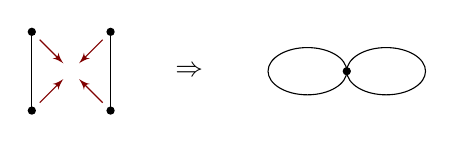
\begin{tikzpicture}
    \node [circ] at (0, 0) {};
    \node [circ] at (1, 0) {};
    \node [circ] at (1, 1) {};
    \node [circ] at (0, 1) {};
    \draw (0, 0) -- (0, 1);
    \draw (1, 0) -- (1, 1);

    \draw [-latex', mred] (0.1, 0.1) -- (0.4, 0.4);
    \draw [-latex', mred] (0.1, 0.9) -- (0.4, 0.6);
    \draw [-latex', mred] (0.9, 0.1) -- (0.6, 0.4);
    \draw [-latex', mred] (0.9, 0.9) -- (0.6, 0.6);

    \node at (2, 0.5) {$\Rightarrow$};
    \begin{scope}[shift={(4, 0.5)}]
      \node [circ] at (0, 0) {};

      \draw (0.5, 0) ellipse (0.5 and 0.3);
      \draw (-0.5, 0) ellipse (0.5 and 0.3);
    \end{scope}
  \end{tikzpicture}
\end{center}
Similarly, at order $\lambda^2$, we have a diagram
\begin{center}
  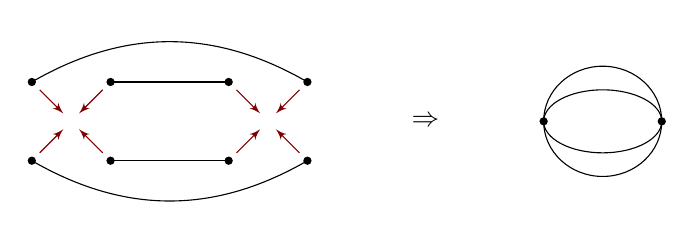
\begin{tikzpicture}
    \node [circ] at (0, 0) {};
    \node [circ] at (1, 0) {};
    \node [circ] at (1, 1) {};
    \node [circ] at (0, 1) {};

    \node [circ] at (2.5, 0) {};
    \node [circ] at (3.5, 0) {};
    \node [circ] at (3.5, 1) {};
    \node [circ] at (2.5, 1) {};

    \draw (1, 0) -- (2.5, 0);
    \draw (1, 1) -- (2.5, 1);

    \draw (0, 0) edge [bend right] (3.5, 0);
    \draw (0, 1) edge [bend left] (3.5, 1);

    \draw [-latex', mred] (0.1, 0.1) -- (0.4, 0.4);
    \draw [-latex', mred] (0.1, 0.9) -- (0.4, 0.6);
    \draw [-latex', mred] (0.9, 0.1) -- (0.6, 0.4);
    \draw [-latex', mred] (0.9, 0.9) -- (0.6, 0.6);

    \begin{scope}[shift={(2.5, 0)}]
      \draw [-latex', mred] (0.1, 0.1) -- (0.4, 0.4);
      \draw [-latex', mred] (0.1, 0.9) -- (0.4, 0.6);
      \draw [-latex', mred] (0.9, 0.1) -- (0.6, 0.4);
      \draw [-latex', mred] (0.9, 0.9) -- (0.6, 0.6);
    \end{scope}

    \node at (5, 0.5) {$\Rightarrow$};
    \begin{scope}[shift={(6.5, 0.5)}]
      \node [circ] at (0, 0) {};
      \node [circ] at (1.5, 0) {};
      \draw (0.75, 0) ellipse (0.75 and 0.7);
      \draw (0.75, 0) ellipse (0.75 and 0.4);
    \end{scope}
  \end{tikzpicture}
\end{center}
Note that in the way we are counting diagrams in Wick's theorem means we consider the following diagrams to be distinct:
\begin{center}
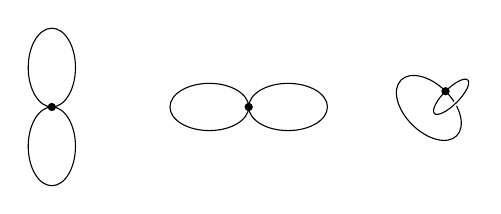
\begin{tikzpicture}
    \node [circ] at (0, 0) {};

    \draw (0, 0.5) ellipse (0.3 and 0.5);
    \draw (0, -0.5) ellipse (0.3 and 0.5);

    \begin{scope}[shift={(2.5, 0)}]
      \node [circ] at (0, 0) {};

      \draw (0.5, 0) ellipse (0.5 and 0.3);
      \draw (-0.5, 0) ellipse (0.5 and 0.3);
    \end{scope}

    \begin{scope}[shift={(5, 0.2)}, rotate=135]
    \draw (0, 0.3) ellipse (0.5 and 0.3);
    \draw [ultra thick, white] (-0.1, 0) ellipse (0.1 and 0.3);
    \draw (-0.1, 0) ellipse (0.1 and 0.3);

    \node [circ] at (0, 0) {};
    \end{scope}
  \end{tikzpicture}
\end{center}
However, \emph{topologically}, these are the same diagrams, and we don't want to count them separately. Combinatorially, these diagrams can be obtained from each other by permuting the outgoing edges at each vertex, or by permuting the vertices. In other words, in the ``expanded view'', when we group our vertices as
\begin{center}
  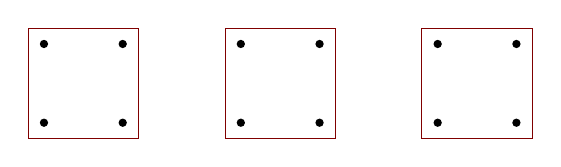
\begin{tikzpicture}
    \node [circ] at (0, 0) {};
    \node [circ] at (1, 0) {};
    \node [circ] at (1, 1) {};
    \node [circ] at (0, 1) {};
    \draw [mred] (-0.2, -0.2) rectangle (1.2, 1.2);

    \node [circ] at (2.5, 0) {};
    \node [circ] at (3.5, 0) {};
    \node [circ] at (3.5, 1) {};
    \node [circ] at (2.5, 1) {};
    \draw [mred] (2.3, -0.2) rectangle (3.7, 1.2);

    \node [circ] at (5, 0) {};
    \node [circ] at (6, 0) {};
    \node [circ] at (6, 1) {};
    \node [circ] at (5, 1) {};
    \draw [mred] (4.8, -0.2) rectangle (6.2, 1.2);
  \end{tikzpicture}
\end{center}
we are allowed to permute the vertices within each block, or permute the blocks themselves. We let $D_n$ be the set of all graphs, and $G_n$ be the group consisting of these ``allowed'' permutations. This $G_n$ is a semi-direct product $(S_4)^n \rtimes S_n$. Then by some combinatorics,
\[
  |D_n| = \frac{(4n)!}{4^n(2n)!},\quad |G_n| = (4!)^n n!.
\]
Recall that $|D_n|$ is the number Wick's theorem gives us, and we now see that $\frac{1}{|G_n|}$ happens to be the factor we obtained from expanding the exponential. Of course, this isn't a coincidence --- we chose to put $\frac{\lambda}{4!}$ instead of, say, $\frac{\lambda}{4}$ in front of the $\phi^4$ term so that this works out.

We can now write the asymptotic series as
\[
  \frac{\mathcal{Z}(m^2, \lambda)}{\mathcal{Z}(m^2, 0)} \sim \sum_{n = 0}^N \frac{|D_n|}{|G_n|} \left(\frac{-\hbar \lambda}{m^4}\right)^n.
\]
It turns out a bit of pure mathematics will allow us to express this in terms of the graphs up to topological equivalence. By construction, two graphs are topologically equivalent if they can be related to each other via $G_n$. In other words, the graphs correspond to the set of \term{orbits} $\mathcal{O}_n$ of $D_n$ under $G_n$. For $n = 1$, there is only one graph up to topological equivalence, so $|\mathcal{O}_1| = 1$. It is not hard to see that $|\mathcal{O}_2| = 3$.

In general, each graph $\Gamma$ has some \emph{automorphisms} that fix the graph. For example, in the following graph:
\begin{center}
  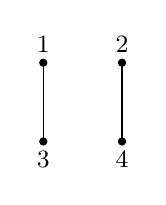
\begin{tikzpicture}
    \node [circ] at (0, 0) {};
    \node [circ] at (1, 0) {};
    \node [circ] at (1, 1) {};
    \node [circ] at (0, 1) {};

    \node [below] at (0, 0) {\small $3$};
    \node [below] at (1, 0) {\small $4$};
    \node [above] at (1, 1) {\small $2$};
    \node [above] at (0, 1) {\small $1$};

    \draw (0, 0) -- (0, 1);
    \draw (1, 0) -- (1, 1);
  \end{tikzpicture}
\end{center}
we see that the graph is preserved by the permutations $(1\; 3)$, $(2\; 4)$ and $(1\; 2)(3\; 4)$. In general, the \term{automorphism group} \term{$\Aut(\Gamma)$} is the subgroup of $G_n$ consisting of all permutations that preserve the graph $\Gamma$. In this case, $\Aut(\Gamma)$ is generated by the above three permutations, and $|\Aut(\Gamma)| = 8$.

Recall from IA Groups that the \emph{orbit-stabilizer theorem} tells us
\[
  \frac{|D_n|}{|G_n|} = \sum_{\Gamma \in \mathcal{O}_n} \frac{1}{|\Aut(\Gamma)|}.
\]
Thus, if we write
\[
  \mathcal{O} = \bigcup_{n \in \N} \mathcal{O}_n,
\]
then we have
\[
  \frac{\mathcal{Z}(m^2, \lambda)}{\mathcal{Z}(m^2, 0)} \sim \sum_{\Gamma \in \mathcal{O}} \frac{1}{|\Aut(\Gamma)|} \left(\frac{-\hbar \lambda}{m^4}\right)^n,
\]
where the $n$ appearing in the exponent is the number of vertices in the graph $\Gamma$.

The last loose end to tie up is the factor of $\left(\frac{-\hbar \lambda}{m^4}\right)^n$ appearing in the sum. While this is a pretty straightforward thing to come up with in this case, for more complicated fields with more interactions, we need a better way of figuring out what factor to put there.

If we look back at how we derived this factor, we had a factor of $-\frac{\lambda}{\hbar}$ coming from each interaction vertex, whereas when computing the correlation functions $\bra \phi^{4n}\ket$, every edge contributes a factor of $\hbar m^{-2}$ (since, in the language we expressed Wick's theorem, we had $M = m^2$). Thus, we can imagine this as saying we have a propagator
\begin{center}
  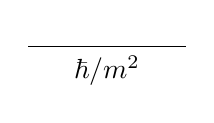
\begin{tikzpicture}
    \draw (0, 0) -- (2, 0) node [pos=0.5, below] {$\hbar/m^2$} node [pos=0.5, above] { };
  \end{tikzpicture}
\end{center}
and a vertex
\begin{center}
  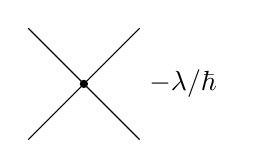
\begin{tikzpicture}[scale=0.707]
    \draw (0, 0) -- (2, 2);
    \draw (0, 2) -- (2, 0);
    \node [circ] at (1, 1) {};
    \node [right] at (2, 1) {$-\lambda /\hbar$};
  \end{tikzpicture}
\end{center}
Note that the negative sign appears because we have $e^{-S}$ in ``Euclidean'' QFT. In Minkowski spacetime, we have a factor of $-i$ instead.

After all this work, we can now expand the partition function as
\[\arraycolsep=0.25em\def\arraystretch{2.2}
  \begin{array}{ccccccccccccc}
  \displaystyle\frac{\mathcal{Z}(m^2, \lambda)}{\mathcal{Z}(m^2, 0)} & \sim &
  \begin{tikzpicture}[eqpic]
    \node {$\emptyset$};
  \end{tikzpicture} &+&
  \begin{tikzpicture}[eqpic]
    \node [circ] at (0, 0) {};

    \draw (0, 0.5) ellipse (0.3 and 0.5);
    \draw (0, -0.5) ellipse (0.3 and 0.5);
  \end{tikzpicture}
  &+&
  \begin{tikzpicture}[eqpic]
    \node [circ] at (0, 0) {};
    \node [circ] at (1.5, 0) {};
    \draw (0.75, 0) ellipse (0.75 and 0.7);
    \draw (0.75, 0) ellipse (0.75 and 0.4);
  \end{tikzpicture}
  &+&
  \begin{tikzpicture}[eqpic]
    \node [circ] at (0, 0) {};
    \node [circ] at (1, 0) {};
    \draw (-0.2, 0) ellipse (0.2 and 0.5);
    \draw (0.5, 0) ellipse (0.5 and 0.3);
    \draw (1.2, 0) ellipse (0.2 and 0.5);
  \end{tikzpicture}
  &+&
  \begin{tikzpicture}[eqpic]
    \node [circ] at (0, 0) {};

    \draw (0, 0.5) ellipse (0.3 and 0.5);
    \draw (0, -0.5) ellipse (0.3 and 0.5);

    \node [circ] at (0.7, 0) {};

    \draw (0.7, 0.5) ellipse (0.3 and 0.5);
    \draw (0.7, -0.5) ellipse (0.3 and 0.5);
  \end{tikzpicture}
  &+&
  \cdots\\
  && 1 &+& \displaystyle\frac{-\lambda \hbar}{m^4} \frac{1}{8} &+& \displaystyle\frac{\lambda^2 \hbar^2}{m^8} \frac{1}{48} &+& \displaystyle\frac{\lambda^2 \hbar^2}{m^8} \frac{1}{16} &+& \displaystyle\frac{\lambda^2 \hbar^2}{m^8} \frac{1}{128} &+& \cdots
\end{array}
\]

In generally, if we have a theory with several fields with propagators of value $\frac{1}{P_i}$, and many different interactions with coupling constants $\lambda_\alpha$, then
\[
  \frac{\mathcal{Z}(\{\lambda_\alpha\})}{ \mathcal{Z}(\{0\})} \sim \sum_{\Gamma \in \mathcal{O}} \frac{1}{|\Aut \Gamma|} \frac{\prod_\alpha \lambda_\alpha^{|v_\alpha(\Gamma)|}}{\prod_i |P_i|^{|e_i(\Gamma)|}} \hbar^{E(\Gamma) - V(\Gamma)},
\]
where
\begin{itemize}
  \item $e_i(\Gamma)$ is the number of edges of type $i$ in $\Gamma$;
  \item $v_\alpha(\Gamma)$ is the number of vertices of type $\alpha$ in $\Gamma$;
  \item $V(\Gamma)$ is the number of vertices in total; and
  \item $E(\Gamma)$ the total number of edges.
\end{itemize}
There are a few comments we can make. Usually, counting \emph{all} graphs is rather tedious. Instead, we can consider the quantity
\[
  \log (\mathcal{Z}/\mathcal{Z}_0).
\]
This is the sum of all \emph{connected} graphs. For example, we can see that the term for the two-figure-of-eight is just the square of the term for a single figure-of-eight times the factor of $\frac{1}{2!}$, and one can convince oneself that this generalizes to arbitrary combinations.

In this case, we can simplify the exponent of $\hbar$. In general, by Euler's theorem, we have
\[
  E - V = L - C,
\]
where $L$ is the number of loops in the graph, and $C$ is the number of connected components. In the case of $\log (\mathcal{Z}/\mathcal{Z}_0)$, we have $C = 1$. Then the factor of $\hbar$ is just $\hbar^{L - 1}$. Thus, the more loops we have, the less it contributes to the sum.

It is not difficult to see that if we want to compute correlation functions, say $\bra \phi^2\ket$, then we should consider graphs with two external vertices. Note that in this case, when computing the combinatorial factors, the automorphisms of a graph are required to fix the external vertices. To see this mathematically, note that the factors in
\[
  \frac{1}{|G_n|} = \frac{1}{(4!)^n n!}
\]
came from Taylor expanding $\exp$ and the coefficient $\frac{1}{4!}$ of $\phi^4$. We do not get these kinds of factors from $\phi^2$ when computing
\[
  \int \d \phi\; \phi^2 e^{-S[\phi]}.
\]
Thus, we should consider the group of automorphisms that fix the external vertices to get the right factor of $\frac{1}{|G_n|}$.

Finally, note that Feynman diagrams don't let us compute exact answers in general. Even if we had some magical means to compute all terms in the expansions using Feynman diagrams, if we try to sum all of them up, it will diverge! We only have an asymptotic series, not a Taylor series. However, it turns out in some special theories, the leading term is the \emph{exact} answer! The tail terms somehow manage to all cancel each other out. For example, this happens for supersymmetry theories, but we will not go into details.

\subsection{An effective theory}
We now play with another toy theory. Suppose we have two scalar fields $\phi, \chi \in \R$, and consider the action
\[
  S(\phi, \chi) = \frac{m^2}{2}\phi^2 + \frac{M^2}{2} \chi^2 + \frac{\lambda}{4} \phi^2 \chi^2.
\]
For convenience, we will set $\hbar = 1$. We have Feynman rules
\begin{center}
  \makecenter{
  \begin{tikzpicture}
    \draw (0, 0) -- (2, 0) node [pos=0.5, below] {$1/m^2$} node [pos=0.5, above] { };
  \end{tikzpicture}}\quad\quad
  \makecenter{\begin{tikzpicture}
    \draw [dashed] (0, 0) -- (2, 0) node [pos=0.5, below] {$1/M^2$} node [pos=0.5, above] { };
  \end{tikzpicture}}
\end{center}
with a vertex
\begin{center}
  \begin{tikzpicture}[scale=0.707]
    \draw (0, 0) -- (2, 2);
    \draw [dashed] (0, 2) -- (2, 0);
    \node [circ] at (1, 1) {};
    \node [right] at (2, 1) {$-\lambda$};
  \end{tikzpicture}
\end{center}
We can use these to compute correlation functions and expectation values. For example, we might want to compute
\[
  \log (\mathcal{Z}/\mathcal{Z}_0).
\]
We have a diagram that looks like
\[\everymath{\displaystyle}\arraycolsep=0.17em\def\arraystretch{2.2}
  \begin{array}{ccccccccccc}
  \displaystyle\log \left(\frac{\mathcal{Z}(m^2, \lambda)}{\mathcal{Z}(m^2, 0)}\right) & \sim &
  \begin{tikzpicture}[eqpic]
    \node [circ] at (0, 0) {};

    \draw [dashed] (0, 0.5) ellipse (0.3 and 0.5);
    \draw (0, -0.5) ellipse (0.3 and 0.5);
  \end{tikzpicture}
  &+&
  \begin{tikzpicture}[eqpic]
    \node [circ] at (0, 0) {};
    \node [circ] at (1, 0) {};
    \draw (-0.2, 0) ellipse (0.2 and 0.5);
    \draw [dashed] (0.5, 0) ellipse (0.5 and 0.3);
    \draw (1.2, 0) ellipse (0.2 and 0.5);
  \end{tikzpicture}
  &+&
  \begin{tikzpicture}[eqpic]
    \node [circ] at (0, 0) {};
    \node [circ] at (1, 0) {};
    \draw [dashed] (-0.2, 0) ellipse (0.2 and 0.5);
    \draw (0.5, 0) ellipse (0.5 and 0.3);
    \draw [dashed] (1.2, 0) ellipse (0.2 and 0.5);
  \end{tikzpicture}
  &+&
  \begin{tikzpicture}[eqpic]
    \node [circ] at (0, 0) {};
    \node [circ] at (1.5, 0) {};
    \draw [dashed] (0.75, 0) ellipse (0.75 and 0.7);
    \draw (0.75, 0) ellipse (0.75 and 0.4);
  \end{tikzpicture}
  &+&
  \cdots\\
  && \frac{-\lambda}{4m^2 M^2} &+& \frac{\lambda^2}{16 m^4 M^4} &+& \frac{\lambda^2}{16 m^4 M^4} &+& \frac{\lambda^2}{8 m^4 M^4} &+& \cdots\\
\end{array}
\]
We can also try to compute $\bra \phi^2\ket$. To do so, we consider diagrams with two vertices connected to a solid line:
\begin{center}
  \begin{tikzpicture}
    \draw (0, 0) node [circ] {} -- (2, 0);
  \end{tikzpicture}
\end{center}
The relevant diagrams are
\[\everymath{\displaystyle}\arraycolsep=0.3em\def\arraystretch{2.2}
  \begin{array}{ccccccccccccc}
  \displaystyle \bra \phi^2 \ket &\sim&
  \begin{tikzpicture}[eqpic]
    \node [circ] at (0, 0) {};
    \node [circ] at (0, -2) {};
    \draw (0, 0) -- (0, -2);
  \end{tikzpicture}
  &+&
  \begin{tikzpicture}[eqpic]
    \node [circ] at (0, 0) {};
    \node [circ] at (0, -2) {};
    \draw (0, 0) -- (0, -2);

    \node [circ] at (0, -1) {};

    \draw [dashed] (0.4, -1) ellipse (0.4 and 0.25);
  \end{tikzpicture}
  &+&
  \begin{tikzpicture}[eqpic]
    \node [circ] at (0, 0) {};
    \node [circ] at (0, -2) {};
    \draw (0, 0) -- (0, -2);

    \node [circ] at (0, -0.667) {};
    \node [circ] at (0, -1.333) {};

    \draw [dashed] (0.4, -0.667) ellipse (0.4 and 0.25);
    \draw [dashed] (0.4, -1.333) ellipse (0.4 and 0.25);
  \end{tikzpicture}
  &+&
  \begin{tikzpicture}[eqpic]
    \node [circ] at (0, 0) {};
    \node [circ] at (0, -2) {};
    \draw (0, 0) -- (0, -2);

    \node [circ] at (0, -0.667) {};
    \node [circ] at (0, -1.333) {};

    \draw [dashed] (0, -1) ellipse (0.333 and 0.333);
  \end{tikzpicture}
  &+&
  \begin{tikzpicture}[eqpic]
    \node [circ] at (0, 0) {};
    \node [circ] at (0, -2) {};
    \draw (0, 0) -- (0, -2);
    \node [circ] at (0, -1) {};

    \draw [dashed] (0.4, -1) ellipse (0.4 and 0.25);
    \node [circ] at (0.8, -1) {};

    \draw (1.2, -1) ellipse (0.4 and 0.25);
  \end{tikzpicture}
  &+&
  \cdots\\
  && \frac{1}{m^2} &+& \frac{-\lambda}{2m^4 M^4} &+& \frac{\lambda^2}{4m^6 M^4} &+& \frac{\lambda^2}{2m^6 M^4} &+& \frac{\lambda^2}{4m^6 M^4} &+& \cdots\\
\end{array}
\]
Let's arrive at this result in a different way. Suppose we think of $\chi$ as ``heavy'', so we cannot access it directly using our experimental equipment. In particular, if we're only interested in the correlation functions that depend only on $\phi$, then we could try to ``integrate out'' $\chi$ first.

Suppose we have a function $f(\phi)$, and consider the integral
\[
  \int_{\R^2} \d \phi\;\d \chi\; f(\phi) e^{-S(\phi, \chi)/\hbar} = \int_\R \d \phi \left(f(\phi) \int_\R \d \chi\;e^{-S(\phi, \chi)/\hbar}\right).
\]
We define the \term{effective action} for $\phi$, $S_{\mathrm{eff}}(\phi)$ by
\[
  S_{\mathrm{eff}}(\phi) = -\hbar \log \left(\int_\R \d \chi\; e^{-S(\phi, \chi)/\hbar}\right).
\]
Then the above integral becomes
\[
  \int_\R \d \phi\; f(\phi) e^{-S_{\mathrm{eff}}(\phi)/\hbar}.
\]
So doing any computation with $\phi$ only is equivalent to pretending $\chi$ doesn't exist, and using this effective potential instead.


In general, the integral is very difficult to compute, and we can only find an asymptotic series for the effective action. However, in this very particular example, we have chosen $S$ such that it is only quadratic in $\chi$, and one can compute to get
\[
  \int_\R \d \chi\; e^{-S(\phi, \chi)/\hbar} = e^{-m^2 \phi^2/2\hbar} \sqrt{\frac{2\pi \hbar}{M^2 + \lambda \phi^2/2}}.
\]
Therefore we have
\begin{align*}
  S_{\mathrm{eff}}(\phi) &= \frac{m^2}{2}\phi^2 + \frac{\hbar}{2} \log \left(1 + \frac{\lambda \phi^2}{2M^2}\right) + \frac{\hbar}{2} \log \left(\frac{M^2}{2\pi \hbar}\right)\\
  &= \left(\frac{m^2}{2} + \frac{\hbar \lambda}{4M^2}\right)\phi^2 - \frac{\hbar \lambda^2}{16 M^4} \phi^4 + \frac{\hbar \lambda^3}{48 M^6} \phi^6 + \cdots + \frac{\hbar}{2} \log \left(\frac{M^2}{2\pi \hbar}\right)\\
  &= \frac{m_{\mathrm{eff}}^2}{2} \phi^2 + \frac{\lambda_4}{4!} \phi^4 + \frac{\lambda_6}{6!} \phi^6 + \cdots + \frac{\hbar}{2} \log \left(\frac{M^2}{2\pi \hbar}\right),
\end{align*}
where
\[
  \lambda_{2k} = (-1)^{k + 1} \frac{\hbar (2k)!}{2^{k + 1}k!} \frac{\lambda^k}{M^{2k}}.
\]
We see that once we integrated out $\chi$, we have generated an \emph{infinite series} of new interactions for $\phi$ in $S_{\mathrm{eff}} (\phi)$. Moreover, the mass also shifted as
\[
  m^2 \mapsto m^2_{\mathrm{eff}} = m^2 + \frac{\hbar \lambda}{2M^4}.
\]
It is important to notice that the new vertices generated are \emph{quantum effects}. They vanish as $\hbar \to 0$ (they happen to be linear in $\hbar$ here, but that is just a coincidence). They are also suppressed by powers of $\frac{1}{M^2}$. So if $\chi$ is very very heavy, we might think these new couplings have very tiny effects.

This is a very useful technique. If the universe is very complicated with particles at very high energies, then it would be rather hopeless to try to account for all of the effects of the particles we cannot see. In fact, it is impossible to know about these very high energy particles, as their energy are too high to reach. All we can know about them is their incarnation in terms of these induced couplings on lower energy fields.

A few things to note:
\begin{itemize}
  \item The original action had a $\Z_2 \times \Z_2$ symmetry, given by $(\phi, \chi) \mapsto (\pm \phi, \pm \chi)$. This symmetry is preserved, and we do not generate any vertices with odd powers of $\phi$.
  \item The field $S_{\mathrm{eff}}(\phi)$ also contains a field independent term
    \[
      \frac{\hbar}{2} \log \left(\frac{M^2}{2\pi \hbar}\right).
    \]
    This plays no role in correlation functions $\bra f(\phi)\ket$. Typically, we are just going to drop it. However, this is one of the biggest problem in physics. This term contributes to the cosmological constant, and the scales that are relevant to this term are much larger than the actual observed cosmological constant. Thus, to obtain the observed cosmological constant, we must have some magic cancelling of these cosmological constants.
  \item In this case, passing to the effective action produced a lot of \emph{new} interactions. However, if we already had a complicated theory, e.g.\ when we started off with an effective action, and then decided to integrate out more things, then instead of introducing new interactions, the effect of this becomes \emph{shifting} the coupling constants, just as we shifted the mass term.
\end{itemize}

In general, how can we compute the effective potential? We are still computing an integral of the form
\[
  \int_\R \d \chi\; e^{-S(\phi, \chi)/\hbar},
\]
so our previous technique of using Feynman diagrams should still work. We will treat $\phi$ as a constant in the theory. So instead of having a vertex that looks like
\begin{center}
  \begin{tikzpicture}[scale=0.707]
    \draw (0, 0) -- (2, 2);
    \draw [dashed] (0, 2) -- (2, 0);
    \node [circ] at (1, 1) {};
    \node [right] at (2, 1) {$-\lambda$};
  \end{tikzpicture}
\end{center}
we drop all the $\phi$ lines and are left with
\begin{center}
  \begin{tikzpicture}[scale=0.707]
    \draw [dashed] (0, 2) -- (2, 0);
    \node [circ] at (1, 1) {};
    \node [right] at (2, 1) {$-\lambda \phi^2$};
  \end{tikzpicture}
\end{center}
But actually, this would be rather confusing. So instead what we do is that we still draw the solid $\phi$ lines, but whenever such a line appears, we have to terminate the line immediately, and this contributes a factor of $\phi$:
\begin{center}
  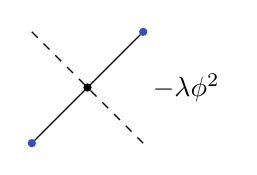
\begin{tikzpicture}[scale=0.707]
    \draw (0, 0) node [circ, mblue] {} -- (2, 2) node [circ, mblue] {};
    \draw [dashed] (0, 2) -- (2, 0);
    \node [circ] at (1, 1) {};
    \node [right] at (2, 1) {$-\lambda \phi^2$};
  \end{tikzpicture}
\end{center}
For our accounting purposes, we will say the internal vertex contributes a factor of $-\frac{\lambda}{2}$ (since the automorphism group of this vertex has order $2$, and the action had $\frac{\lambda}{4}$), and each terminating blue vertex contributes a factor of $\phi$.

Since we have a ``constant'' term $\frac{m^2}{2} \phi^2$ as well, we need to add one more diagram to account for that. We allow a single edge of the form
\begin{center}
  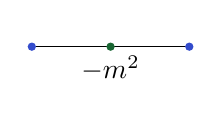
\begin{tikzpicture}
    \draw (0, 0) node [mblue, circ] {} -- (2, 0) node [mblue, circ] {} node [pos=0.5, below] {$-m^2$} node [pos=0.5, above] { };
    \node [circ, mgreen] at (1, 0) {};
  \end{tikzpicture}
\end{center}
With these ingredients, we can compute the effective potential as follows:
\[\everymath{\displaystyle}\arraycolsep=0.3em\def\arraystretch{2.2}
  \begin{array}{ccccccccccc}
    \displaystyle -S_{\mathrm{eff}}(\phi) &\sim&
  \begin{tikzpicture}[eqpic]
    \node [circ, mblue] at (0, 0) {};
    \node [circ, mblue] at (0, -2) {};
    \draw (0, 0) -- (0, -2);
  \end{tikzpicture}
  &+&
  \begin{tikzpicture}[eqpic]
    \node [circ, mblue] at (0, 0) {};
    \node [circ, mblue] at (0, -2) {};
    \draw (0, 0) -- (0, -2);

    \node [circ] at (0, -1) {};

    \draw [dashed] (0.4, -1) ellipse (0.4 and 0.25);
  \end{tikzpicture}
  &+&
  \begin{tikzpicture}[eqpic]
    \draw (0, 0) node [circ, mblue] {} -- +(0, -1) node [circ] {} -- +(0, -2) node [circ, mblue] {};
    \draw (0.8, 0) node [circ, mblue] {} -- +(0, -1) node [circ] {} -- +(0, -2) node [circ, mblue] {};
    \draw [dashed] (0.4, -1) ellipse (0.4 and 0.25);
  \end{tikzpicture}
  &+&
  \begin{tikzpicture}[eqpic]
    \draw (0, 0) node [circ, mblue] {} -- +(0, -1) node [circ] {} -- +(0, -2) node [circ, mblue] {};
    \draw (0.8, 0) node [circ, mblue] {} -- +(0, -1) node [circ] {} -- +(0, -2) node [circ, mblue] {};
    \draw (0.4, 0.25) node [circ, mblue] {} -- +(0, -1) node [circ] {} -- +(0, -2) node [circ, mblue] {};
    \draw [dashed] (0.4, -1) ellipse (0.4 and 0.25);
  \end{tikzpicture}
  &+&
  \cdots\\
  && \frac{-m^2}{2}\phi^2 &+& \frac{-\lambda}{4 M^2} \phi^2 &+& \frac{\lambda^2 \phi^4}{16 M^4} &+& \frac{- \lambda^3 \phi^6}{48 M^6} &+& \cdots
\end{array}
\]
These are just the terms we've previously found. There are, again, a few things to note
\begin{itemize}
  \item The diagram expansion is pretty straightforward in this case, because we started with a rather simple interacting theory. More complicated examples will have diagram expansions that are actually interesting.
  \item We only sum over connected diagrams, as $S_{\mathrm{eff}}$ is the logarithm of the integral.
  \item We see that the new/shifted couplings in $S_{\mathrm{eff}} (\phi)$ are generated by \emph{loops} of $\chi$ fields.
  \item When we computed the effective action directly, we had a ``cosmological constant'' term $\frac{\hbar}{2} \log\left(\frac{M^2}{2 \pi \hbar}\right)$, but this doesn't appear in the Feynman diagram calculations. This is expected, since when we developed our Feynman rules, what it computed for us was things of the form $\log (\mathcal{Z}/\mathcal{Z}_0)$, and the $\mathcal{Z}_0$ term is that ``cosmological constant''.
\end{itemize}

\begin{eg}
  We can use the effective potential to compute $\bra \phi^2 \ket$:
  \[\everymath{\displaystyle}\arraycolsep=0.3em\def\arraystretch{2.2}
    \begin{array}{ccccccc}
      \displaystyle \bra \phi^2 \ket &\sim&
      \begin{tikzpicture}[eqpic]
        \node [circ] at (0, 0) {};
        \node [circ] at (0, -2) {};
        \draw (0, 0) -- (0, -2);
      \end{tikzpicture}
      &+&
      \begin{tikzpicture}[eqpic]
        \node [circ] at (0, 0) {};
        \node [circ] at (0, -2) {};
        \draw (0, 0) -- (0, -2);

        \node [circ] at (0, -1) {};

        \draw (0.4, -1) ellipse (0.4 and 0.25);
      \end{tikzpicture}
      &+&
      \cdots\\
      && \frac{1}{m_{\mathrm{eff}}^2} &+& \frac{-\lambda}{2m^6_{\mathrm{eff}}} &+& \cdots
    \end{array}
  \]
  We can see that this agrees with our earlier calculation correct to order $\lambda^2$.
\end{eg}

At this moment, this is not incredibly impressive, since it takes a lot of work to compute $S_{\mathrm{eff}}(\phi)$. But the computation of $S_{\mathrm{eff}}(\phi)$ can be reused to compute any correlation involving $\phi$. So if we do many computations with $\phi$, then we we can save time.

But the point is not that this saves work. The point is that this is what we do when we do physics. We can never know if there is some really high energy field we can't reach with our experimental apparatus. Thus, we can only assume that the actions we discover experimentally are the effective actions coming from integrating out some high energy fields.

\subsection{Fermions}
So far, we have been dealing with Bosons. These particles obey Bose statistics, so different fields $\phi$ commute with each other. However, we want to study Fermions as well. This would involve variables that anti-commute with each other. When we did canonical quantization, this didn't pose any problem to our theory, because fields were represented by operators, and operators can obey any commutation or anti-commutation relations we wanted them to. However, in the path integral approach, our fields are actual numbers, and they are forced to commute.

So how can we take care of fermions in our theory? We cannot actually use path integrals, as these involves things that commute. Instead, we will now treat the fields as formal symbols.

The theory is rather trivial if there is only one field. So let's say we have many fields $\theta_1, \cdots, \theta_n$. Then a ``function'' of these fields will be a formal polynomial expression in the symbols $\theta_1, \cdots, \theta_n$ subject to the relations $\theta_i \theta_j = - \theta_j \theta_i$. So, for example, the action might be
\[
  S[\theta_1, \theta_2] = \frac{1}{2} m^2 \theta_1 \theta_2 = - \frac{1}{2}m^2 \theta_2 \theta_1.
\]
Now the path integral is defined as
\[
  \int \d \theta_1 \cdots \d \theta_n \; e^{-S[\theta_1, \ldots, \theta_n]}.
\]
There are two things we need to make sense of --- the exponential, and the integral.

The exponential is easy. In general, for any analytic function $f: \R \to \R$ (or $f: \C \to \C$), we can write it as a power series
\[
  f(x) = \sum_{i = 0}^\infty a_i x^i.
\]
Then for any polynomial $p$ in the fields, we can similarly define
\[
  f(p) = \sum_{i = 0}^\infty a_i p^i.
\]
Crucially, this expression is a \emph{finite} sum, since we have only finitely many fields, and any monomial in the fields of degree greater than the number of fields must vanish by anti-commutativity.

\begin{eg}
  \begin{align*}
    e^{\theta_1 + \theta_2} &= 1 + \theta_1 + \theta_2 + \frac{1}{2}(\theta_1 + \theta_2)^2 + \cdots\\
    &= 1 + \theta_1 + \theta_2 + \frac{1}{2}(\theta_1 \theta_2 + \theta_2 \theta_1)\\
    &= 1 + \theta_1 + \theta_2
  \end{align*}
\end{eg}

How about integration? Since our fields are just formal symbols, and do not represent real/complex numbers, it doesn't make sense to actually integrate it. However, we can still define a linear functional from the space of all polynomials in the fields to the reals (or complexes) that is going to act as integration.

If we have a single field $\theta$, then the most general polynomial expression in $\theta$ is $a + b \theta$. It turns out the correct definition for the ``integral'' is
\[
  \int \d \theta\; (a + b \theta) = b.
\]
This is known as the \term{Berezin integral}.

How can we generalize this to more fields? Heuristically, the rule is that $\int \d \theta$ is an expression that should anti-commute with all fields. Thus, for example,
\begin{align*}
  \int \d \theta_1 \; \d \theta_2\; (3\theta_2 + 2 \theta_1 \theta_2) &= \int \d \theta_1 \left(3 \int \d \theta_2\; \theta_2 + 2 \int \d \theta_2 \; \theta_1 \theta_2\right)\\
  &= \int \d \theta_1 \left(3 - 2 \theta_1 \int \d \theta_2 \; \theta_2\right)\\
  &= \int \d \theta_1 (3 - 2 \theta_1)\\
  &= -2.
\end{align*}
On the other hand, we have
\begin{align*}
  \int \d \theta_1 \; \d \theta_2\; (3\theta_2 + 2 \theta_2 \theta_1) &= \int \d \theta_1 \left(3 \int \d \theta_2\; \theta_2 + 2 \int \d \theta_2 \; \theta_2 \theta_1\right)\\
  &= \int \d \theta_1 \left(3 + 2 \left(\int \d \theta_2 \; \theta_2\right) \theta_1\right)\\
  &= \int \d \theta_1 (3 - 2 \theta_1)\\
  &= 2.
\end{align*}
Formally speaking, we can define the integral by
\[
  \int \d \theta_1 \cdots \d \theta_n\; \theta_n \cdots \theta_1 = 1,
\]
and then sending other polynomials to $0$ and then extending linearly.

When actually constructing a fermion field, we want an action that is ``sensible''. So we would want a mass term $\frac{1}{2} m^2 \theta^2$ in the action. But for anti-commuting variables, this must vanish!

The solution is to imagine that our fields are \emph{complex}, and we have two fields $\theta$ and $\bar{\theta}$. Of course, formally, these are just two formal symbols, and bear no relation to each other. However, we will think of them as being complex conjugates to each other. We can then define the action to be
\[
  S[\bar{\theta}, \theta] = \frac{1}{2} m^2 \bar{\theta} \theta.
\]
Then the partition function is
\[
  \mathcal{Z} = \int \d \theta\; \d \bar{\theta}\; e^{-S(\bar{\theta}, \theta)}.
\]
Similar to the previous computations, we can evaluate this to be
\begin{align*}
  \mathcal{Z} &= \int \d \theta \;\d \bar{\theta}\; e^{-S(\bar{\theta}, \theta)}\\
  &= \int \d \theta \left(\int \d \bar{\theta}\; \left(1 - \frac{1}{2} m^2 \bar{\theta} \theta\right)\right)\\
  &= \int \d \theta \left(\int \d \bar{\theta} - \frac{1}{2} m^2 \left(\int \d \bar{\theta}\; \bar{\theta}\right) \theta \right)\\
  &= \int \d \theta \left(- \frac{1}{2} m^2 \theta\right)\\
  &= -\frac{1}{2} m^2.
\end{align*}

We will need the following formula:
\begin{prop}
  For an invertible $n \times n$ matrix $B$ and $\eta_i, \bar{\eta}_i, \theta^i, \bar{\theta}^i$ independent fermionic variables for $i = 1,\ldots, n$, we have
  \[
    \mathcal{Z}(\eta, \bar{\eta}) = \int \d^n \theta\; \d^n \bar{\theta}\;\exp\left(\bar{\theta}^i B_{ij} \theta^j + \bar{\eta}_i \theta^i + \bar{\theta}^i \eta_i\right) = \det B \exp\left(\bar{\eta}_i (B^{-1})^{ij} \eta_j\right).
  \]
  In particular, we have
  \[
    \mathcal{Z} = \mathcal{Z}(0, 0) = \det B.
  \]
\end{prop}
As before, for any function $f$, we can again define the correlation function
\[
  \bra f(\bar{\theta}, \theta)\ket = \frac{1}{\mathcal{Z}(0, 0)} \int \d^n \theta\; \d^n \bar{\theta}\; e^{-S(\bar{\theta}, \theta)} f(\bar{\theta}, \theta).
\]

Note that usually, $S$ contains even-degree terms only. Then it doesn't matter if we place $f$ on the left or the right of the exponential.

It is an exercise on the first example sheet to prove these, derive Feynman rules, and investigate further examples.
\section{QFT in one dimension (i.e.\ QM)}
\subsection{Quantum mechanics}
In $d = 1$, there are two possible connected, compact manifolds $M$ --- we can have $M = S^1$ or $M = I = [0, 1]$.
\begin{center}
  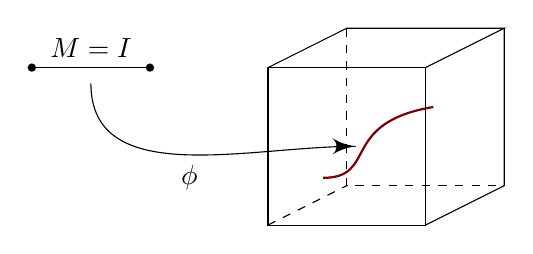
\begin{tikzpicture}
    \draw (0, 0) node [circ] {} -- (1.5, 0) node [circ] {} node [pos=0.5, above] {$M = I$};

    \draw (3, 0) rectangle (5, -2);
    \draw (3, 0) -- (4, 0.5) -- (6, 0.5) -- (5, 0);
    \draw (6, 0.5) -- (6, -1.5) -- (5, -2);
    \draw [dashed] (4, 0.5) -- (4, -1.5) -- (6, -1.5);
    \draw [dashed] (3, -2) -- (4, -1.5);

    \draw (0.75, -0.2) edge [out=270, in=180] (4.1, -1);

    \node at (2, -1.4) {$\phi$};

    \draw [->] (4.099, -1) -- (4.1, -1);

    \draw [thick, mred](3.7, -1.4) .. controls (4.4, -1.4) and (3.9, -0.7) .. (5.1, -0.5);
  \end{tikzpicture}
\end{center}
We will mostly be considering the case where $M = I$. In this case, we need to specify boundary conditions on the field in the path integral, and we will see that this corresponds to providing start and end points to compute matrix elements.

We let $t \in [0, 1]$ be the worldline coordinate parametrizing the field, and we write our field as
\[
  x: I \to N
\]
for some Riemannian manifold $(N, g)$, which we call the \term{target manifold}. If $U\subseteq N$ has coordinates $x^a$ with $a = 1, \cdots, n = \dim (N)$, then we usually write $x^a(t)$ for the coordinates of $x(t)$. The standard choice of action is
\[
  S[x] = \int_I \left(\frac{1}{2} g(\dot{x}, \dot{x}) + V(x)\right)\;\d t,
\]
where $\dot{x}$ is as usual the time derivative, and $V(x)$ is some potential term.

We call this theory a \term{non-linear $\sigma$-model}\index{$\sigma$-model!non-linear}\index{sigma model!non-linear}. This is called $\sigma$-model because when people first wrote this theory down, they used $\sigma$ for the name of the field, and the name stuck. This is non-linear because the term $g(\dot{x}, \dot{x})$ can be very complicated when the metric $g$ if it is not flat. Note that $+V(x)$ is the correct sign for a Euclidean worldline.

Classically, we look for the extrema of $S[x]$ (for fixed end points), and the solutions are given by the solutions to
\[
  \frac{\d^2 x^a}{\d t^2} + \Gamma^a\!_{bc} \dot{x}^b \dot{x}^c = g^{ab} \frac{\partial V}{\partial x^b}.
\]
The left-hand side is just the familiar geodesic equation we know from general relativity, and the right hand term corresponds to some non-gravitational force.

In the case of zero-dimensional quantum field theory, we just wrote down the partition function
\[
  \mathcal{Z} = \int e^{-S},
\]
and assumed it was an interesting thing to calculate. There wasn't really a better option because it is difficult to give a physical interpretation to a zero-dimensional quantum field theory. In this case, we will see that path integrals naturally arise when we try to do quantum mechanics.

To do quantum mechanics, we first pick a Hilbert space $\mathcal{H}$. We usually take it as
\[
  \mathcal{H} = L^2(N, \d \mu),
\]
the space of square-integrable functions on $N$.

To describe dynamics, we pick a Hamiltonian operator $H: \mathcal{H} \to \mathcal{H}$, with the usual choice being
\[
  H = \frac{1}{2} \Delta + V,
\]
where the \term{Laplacian} $\Delta$\index{$\Delta$} is given by
\[
  \Delta = \frac{1}{\sqrt{g}} \partial_a(\sqrt{g} g^{ab} \partial_b).
\]
As usually, the $\sqrt{g}$ refers to the square root of the determinant of $g$.

We will work in the Heisenberg picture. Under this set up, the amplitude for a particle to travel from $x \in N$ to $y \in N$ in time $T$ is given by the \term{heat kernel}\index{$K_T(y, x)$}
\[
  K_T(y, x) = \brak{y} e^{-HT}\bket{x}.
\]
Note that we have $e^{-HT}$ instead of $e^{-iHT}$ because we are working in a Euclidean world. Strictly speaking, this doesn't really make sense, because $\bket{x}$ and $\bket{y}$ are not genuine elements of $\mathcal{H} = L^2(N, \d \mu)$. They are $\delta$-functions, which aren't functions. There are some ways to fix this problem. One way is to see that the above suggests $K_T$ satisfies
\[
  \frac{\partial}{\partial t} K_t(y, x) + H K_t(y, x) = 0,
\]
where we view $x$ as a fixed parameter, and $K_t$ is a function of $y$, so that $H$ can act on $K_t$. The boundary condition is
\[
  \lim_{t \to 0} K_t(y, x) = \delta (y - x),
\]
and this uniquely specifies $K_t$. So we can \emph{define} $K_t$ to be the unique solution to this problem.

We can reconnect this back to the usual quantum mechanics by replacing the Euclidean time $T$ with $it$, and the above equation gives us the \term{Schr\"odinger equation}
\[
  i \frac{\partial K_t}{\partial t} (y, x) = H K_t(y, x).
\]
We first focus on the case where $V = 0$. In the case where $(N, g) = (\R^n, \delta)$, we know from, say, IB Methods, that the solution is given by
\[
  K_t(y, x) = \frac{1}{(2\pi t)^{n/2}} \exp\left(-\frac{|x - y|^2}{2t}\right).
\]
For an arbitrary Riemannian manifold $(N, g)$, it is in general very hard to write down a closed-form expression for $K_t$. However, we can find the asymptotic form
\[
  \lim_{t \to 0} K_t(y, x) \sim \frac{a(x)}{(2\pi t)^{n/2}} \exp\left(- \frac{d(y, x)^2}{2t}\right),
\]
where $d(x, y)$ is the geodesic distance between $x$ and $y$, and $a(x)$ is some invariant of our manifold built from (integrals of) polynomials of the Riemann curvature that isn't too important.

Here comes the magic. We notice that since
\[
  \mathbb{I} = \int \d^n z\; \bket{z} \brak{z}
\]
is the identity operator, we can write
\begin{align*}
  K_{t_1 + t_2} (y, x) &= \brak{y} e^{-TH} \bket{x}\\
  &= \int \d^n z\; \brak{y} e^{-t_1H} \bket{z}\brak{z} e^{-t_2H} \bket{x} \\
  &= \int \d^n z\; K_{t_2}(y, z) K_{t_1}(z, x).
\end{align*}
For flat space, this is just reduces to the formula for convolution of Gaussians. This is the \term{concatenation property} of the heat kernel.

Using this many times, we can break up our previous heat kernel by setting
\[
  \Delta t = \frac{T}{N}
\]
for some large $N \in \N$. Then we have
\[
  K_T(y, x) = \int \prod_{i = 1}^{N - 1} \d^n x_i\; K_{\Delta t} (x_i, x_{i - 1}),
\]
where we conveniently set $x_0 = x$ and $x_N = y$.

The purpose of introducing these $\Delta t$ is that we can now use the asymptotic form of $K_t(y, t)$. We can now say
\begin{multline*}
  \brak{y_1} e^{-HT} \bket{y_0} \\
  = \lim_{N \to \infty} \left(\frac{1}{2\pi \Delta t}\right)^{nN/2} \int \prod_{i = 1}^{N - 1} \d^n x_i\; a(x_i) \exp\left(- \frac{\Delta t}{2}\left(\frac{d(x_{i + 1}, x_i)}{\Delta t}\right)^2\right).
\end{multline*}
This looks more-or-less like a path integral! We now dubiously introduce the path integral measure
\[
  \D x \overset{?}{\equiv} \lim_{N \to \infty} \left(\frac{1}{2\pi \Delta t}\right)^{nN/2} \prod_{i = 1}^{N - 1} \d^n x_i\; a(x_i),
\]
and also assume our map $x(t)$ is at least once-continuously differentiable, so that
\begin{multline*}
  \lim_{N \to \infty} \prod_{i = 1}^{N - 1} \exp\left(-\frac{\Delta t}{2} \left(\frac{d(x_{i + 1}, x_i)}{\Delta t}\right)^2 \right)\\
  \overset{?}{\equiv} \exp\left(-\frac{1}{2} \int \d t\; g(\dot{x}, \dot{x})\right) = \exp(-S[x]).
\end{multline*}
Assuming these things actually make sense (we'll later figure out they don't), we can write
\[
  \brak{y_1} e^{-HT} \bket{y_0} = \int_{\mathcal{C}_T[y_1, y_0]} \D x\; e^{-S[x]},
\]
where $\mathcal{C}_T[y_1, y_0]$ is the space of ``all'' maps $I \to N$ such that $x(0) = y_0$ and $x(1) = y_1$.

Now consider an arbitrary $V \not= 0$. Then we can write
\[
  H = H_0 + V(x),
\]
where $H_0$ is the free Hamiltonian. Then we note that for small $t$, we have
\[
  e^{-Ht} = e^{-H_0t}E^{-V(x)t} + o(t).
\]
Thus, for small $t$, we have
\begin{align*}
  K_t(y, x) &= \brak{y} e^{-Ht}\bket{x}\\
  &\approx \brak{y}e^{-H_0t} e^{-V(x) t}\bket{x}\\
  &\sim \frac{a(x)}{(2\pi t)^{n/2}} \exp\left(- \left(\frac{1}{2} \left(\frac{d(y, x)}{t}\right)^2 + V(x)\right) t\right).
\end{align*}
Then repeating the above derivations will again give us
\[
  \brak{y_1} e^{-HT} \bket{y_0} = \int_{\mathcal{C}_T[y_1, y_0]} \D x\; e^{-S[x]}.
\]

Before we move on to express other things in terms of path integrals, and then realize our assumptions are all wrong, we make a small comment on the phenomena we see here.

Notice that the states $\bket{y_0} \in \mathcal{H}$ and $\brak{y_1} \in \mathcal{H}^*$ we used to evaluate our propagator here arise as boundary conditions on the map $x$. This is a general phenomenon. The co-dimension-$1$ subspaces (i.e.\ subspaces of $M$ of one dimension lower than $M$) are associated to states in our Hilbert space $\mathcal{H}$. Indeed, when we did quantum field theory via canonical quantization, the states corresponded to the state of the universe at some fixed time, which is a co-dimension 1 slice of spacetime.

\subsubsection*{The partition function}
We can naturally interpret a lot of the things we meet in quantum mechanics via path integrals. In statistical physics, we often called the quantity $\Tr_\mathcal{H} (e^{-HT})$ the \term{partition function}. Here we can compute it as
\[
  \Tr_H(e^{-HT}) = \int \d^n y\; \brak{y}e^{-HT} \bket{y}.
\]
Using our path integral formulation, we can write this as
\[
  \Tr_\mathcal{H} (e^{-HT}) = \int \d^n y \int_{C_I[y, y]} \D x\; e^{-S} = \int_{\mathcal{C}_{S^1}} \D x\; e^{-S},
\]
where we integrate over all circles. This is the partition function $\mathcal{Z}(S^1, (N, g, V))$ of our theory. If one is worried about convergence issues, then we would have some problems in this definition. If we work in flat space, then $K_T(y, y) = \brak{y}e^{-HT}\bket{y}$ is independent of $y$. So when we integrate over all $y$, the answer diverges (as long as $K_T(y, y)$ is non-zero). However, we would get a finite result if we had a compact manifold instead.

\subsubsection*{Correlation functions}
More interestingly, we can do correlation functions. We will begin by considering the simplest choice --- local operators.
\begin{defi}[Local operator]\index{local operator}
  A \emph{local operator} $\mathcal{O}(t)$ is one which depends on the values of the fields and finitely many derivatives just at one point $t \in M$.
\end{defi}
We further restrict to local operators that do not depend on derivatives. These are given by functions $\mathcal{O}: N \to \R$, and then by pullback we obtain an operator $\mathcal{O}(x(t))$.

Suppose the corresponding quantum operator is $\hat{\mathcal{O}} = \mathcal{O}(\hat{x})$, characterized by the property
\[
  \hat{\mathcal{O}}\bket{x} = \mathcal{O}(x) \bket{x}.
\]
If we want to evaluate this at time $t$, then we would compute
\[
  \brak{y_1} \hat{\mathcal{O}}(t) \bket{y_0} = \brak{y_1} e^{-H(T - t)} \hat{\mathcal{O}} e^{-Ht} \bket{y_0}.
\]
But, inserting a complete set of states, this is equal to
\begin{multline*}
  \int \d^n x\; \brak{y_1} e^{-H(T - t)}\bket{x} \brak{x}\hat{\mathcal{O}} e^{-Ht} \bket{y} \\
  = \int \d^n x\; \mathcal{O}(x) \brak{y_1} e^{-H(T - t)} \bket{x} \brak{x} e^{-Ht} \bket{y}.
\end{multline*}
Simplifying notation a bit, we can write
\[
  \brak{y_1} \hat{\mathcal{O}}(t) \bket{y_0} = \int \d^n x\; \mathcal{O}(x(t)) \int\limits_{\mathcal{C}_{[T, t]} [y_1, x_t]} \D x\; e^{-S[x]} \int\limits_{\mathcal{C}_{[t, 0]}[x_t, y_0]} \D x\; e^{-S[x]}.
\]
But this is just the same as
\[
  \int\limits_{\mathcal{C}_{[T, 0]}[y_1, y_0]} \D x\; \mathcal{O}(x(t)) e^{-S[x]}.
\]

More generally, suppose we have a sequence of operators $\mathcal{O}_n, \cdots, \mathcal{O}_1$ we want to evaluate at times $T > t_n > t_{n - 1} > \cdots > t_1 > 0$, then by the same argument, we find
\[
  \brak{y_1} e^{-HT}\hat{\mathcal{O}}_n(t_n)\cdots\hat{\mathcal{O}}_1(t_1) \bket{y_0} = \int_{\mathcal{C}_{[0, T]}[y_0, y_1]} \D x\; \mathcal{O}_n(x(t_n)) \cdots \mathcal{O}(x(t_1)) e^{-S[x]}.
\]
Note that it is crucial that the operators are ordered in this way, as one would see if they actually try to prove this. Indeed, the $\hat{\mathcal{O}}_i$ are operators, but the objects in the path integral, i.e.\ the $\mathcal{O}(x(t_i))$ are just functions. Multiplication of operators does not commute, but multiplication of functions does. In general, if $\{t_i\} \in (0, T)$ are a collection of times, then we have
\[
  \int \D x \prod_{i = 1}^n \mathcal{O}_i(x(t_i)) e^{-S[x]} = \brak{y_1} e^{-HT}\mathcal{T} \prod_{i = 1}^n \hat{\mathcal{O}}_i(t_i) \bket{y_0},
\]
where $\mathcal{T}$ denotes the time ordering operator. For example, for $n = 2$, we have
\[
  \mathcal{T} \lbrack \hat{\mathcal{O}}_1(t_1) \hat{\mathcal{O}}_2(t_2)\rbrack = \Theta(t_2 - t_1) \hat{\mathcal{O}}_2(t_2) \hat{\mathcal{O}}_1(t_1) + \Theta(t_1 - t_2) \hat{\mathcal{O}}_1(t_1) \hat{\mathcal{O}}_2(t_2),
\]
where $\Theta$ is the step function.

It is interesting to note that in this path integral formulation, we see that we get non-trivial correlation between operators at different times only because of the kinetic (derivative) term in the action. Indeed, for a free theory, the discretized version of the path integral looked like
\[
  S_{\mathrm{kin}}[x] = \sum_i \frac{1}{2} \left(\frac{x_{i + 1} - x_i}{\Delta t}\right)^2 \Delta t,
\]
Now if we don't have this term, and the action is purely potential:
\[
  S_{\mathrm{pot}}[x] = \sum_i V(x_i),
\]
then the discretized path integral would have factorized into a product of integrals at these sampling points $x_i$. It would follow that for any operators $\{\mathcal{O}_i\}$ that depend only on position, we have
\[
  \left\bra \prod_i \mathcal{O}_i(x(t_i))\right\ket = \prod_i \left\bra \mathcal{O}_i(x(t_i))\right\ket,
\]
and this is incredibly boring. When we work with higher dimensional universes, the corresponding result shows that if there are no derivative terms in the potential, then events at one position in spacetime have nothing to do with events at any other position.

We have already seen this phenomena when we did quantum field theory with perturbation theory --- the interactions between different times and places are given by propagators, and these propagators arise from the kinetic terms in the Lagrangian.

 % Note that in the case of QM, it might not be clear what we are computing when we write $\brak{y_1} \mathcal{O}(t) \bket{y_0}$. But, when we do full-blown quantum field theory, we could, for example, take $\bket{y_1} = \bket{y_0} = \bket{\Omega}$, the vacuum, and $\mathcal{O}(t) = \phi(x) \phi(y)$. Then this two-point correlator is just the propagator we are familiar with!
\subsubsection*{Derivative terms}
We now move on to consider more general functions of the field and its derivative. Consider operators $\mathcal{O}_i(x, \dot{x}, \cdots)$. We might expect that the value of this operator is related to path integrals of the form
\[
  \int \D x\; \mathcal{O}_1(x, \dot{x}, \cdots)|_{t_1} \mathcal{O}_2(x, \dot{x}, \cdots)|_{t_2} e^{-S[x]}
\]
But this can't be right. We were told that one of the most important properties of quantum mechanics is that operators do not commute. In particular, for $p_i = \dot{x}_i$, we had the renowned commutator relation
\[
  [\hat{x}^i, \hat{p}_j] = \delta^i_j.
\]
But in this path integral formulation, we feed in \emph{functions} to the path integral, and it knows nothing about how we order $x$ and $\dot{x}$ in the operators $\mathcal{O}_i$. So what can we do?

The answer to this is really really important. The answer is that path integrals don't work.
\subsubsection*{The path integral measure}
Recall that to express our correlation functions as path integrals, we had to take the limits
\[
  \D x \overset{?}{=} \lim_{N \to \infty} \frac{1}{(2\pi \Delta t)^{nN/2}}\prod_{i = 1}^{N - 1} \d^n x_i a(x_i),
\]
and also
\[
  S[x] \overset{?}{=} \lim_{N \to \infty}\sum_{n = 1}^{N - 1} \frac{1}{2} \left(\frac{x_{n + 1} - x_n}{\Delta t}\right)^2 \Delta t.
\]
Do these actually make sense?

What we are trying to do with these expressions is that we are trying to \emph{regularize} our path integral, i.e.\ find a finite-dimensional approximation of the path integral. For quantum field theory in higher dimensions, this is essentially a lattice regularization.

Before we move on and try to see if this makes sense, we look at another way of regularizing our path integral. To do so, we decompose our field into Fourier modes:
\[
  x^a(t) = \sum_{k \in \Z} x_k^a e^{-2\pi i k t/T},
\]
and then we can obtain a regularized form of the action as
\[
  S_N[x] = \sum_{k = -N}^N \frac{1}{2} k^2 x^a_k x^a_k.
\]
Under this decomposition, we can take the regularized path integral measure to be
\[
  \D_N x = \prod_{|k| \leq N} \d^n x_k.
\]
This is analogous to high-energy cutoff regularization. Now the natural question to ask is --- do the limits
\[
  \lim_{N \to \infty} \int \D_N x,\quad \lim_{N \to \infty} S_N[x]
\]
exist?

The answer is, again: NO! This is in fact not a problem of us not being able to produce limits well. It is a general fact of life that we cannot have a Lebesgue measure on an infinite dimensional inner product space (i.e.\ vector space with an inner product).

Recall the following definition:
\begin{defi}[Lebesgue measure]\index{Lebesgue measure}
  A \emph{Lebesgue measure} $\d \mu$ on an inner product space $V$ obeys the following properties
  \begin{itemize}
    \item For all non-empty open subsets $U \subseteq \R^D$, we have
      \[
        \vol(U) = \int_U \d \mu > 0.
      \]
    \item If $U'$ is obtained by translating $U$, then
      \[
        \vol(U') = \vol(U).
      \]
    \item Every $x \in V$ is contained in at least one open neighbourhood $U_x$ with finite volume.
  \end{itemize}
\end{defi}
note that we don't really need the inner product structure in this definition. We just need it to tell us what the word ``open'' means.

We now prove that there cannot be any Lebesgue measure on an infinite dimensional inner product space.

We first consider the case of a finite-dimensional inner product space. Any such inner product space is isomorphic to $\R^D$ for some $D$. Write $C(L)$ for an open hypercube of side length $L$. By translation in variance, the volume of any two such hypercubes would be the same.

Now we note that given any such hypercube, we can cut it up into $2^D$ hypercubes of side length $L/2$:
\begin{center}
  \makecenter{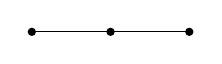
\begin{tikzpicture}
    \draw (0, 0) node [circ] {} -- (2, 0) node [circ] {} node [pos=0.5, circ] {};
  \end{tikzpicture}}
  \quad\quad
  \makecenter{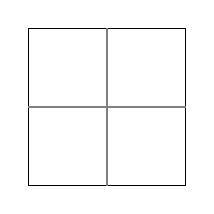
\begin{tikzpicture}
    \draw (0, 0) rectangle (2, 2);
    \draw [gray] (1, 0) -- (1, 2);
    \draw [gray] (0, 1) -- (2, 1);
  \end{tikzpicture}}
  \quad\quad
  \makecenter{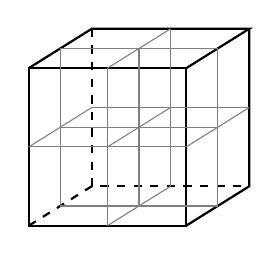
\begin{tikzpicture}
    \draw [thick] (0, 0) rectangle (2, -2);
    \draw [thick] (0, 0) -- (0.8, 0.5) -- (2.8, 0.5) -- (2, 0);
    \draw [thick] (2.8, 0.5) -- (2.8, -1.5) -- (2, -2);
    \draw [dashed, thick] (0.8, 0.5) -- (0.8, -1.5) -- (2.8, -1.5);
    \draw [dashed, thick] (0, -2) -- (0.8, -1.5);

    \draw [gray] (1, 0) -- (1, -2);
    \draw [gray] (0, -1) -- (2, -1);

    \draw [gray] (1.8, 0.5) -- (1.8, -1.5);
    \draw [gray] (0.8, -0.5) -- (2.8, -0.5);

    \draw [gray] (1, 0) -- (1.8, 0.5);
    \draw [gray] (1, -2) -- (1.8, -1.5);

    \draw [gray] (2, -1) -- (2.8, -0.5);
    \draw [gray] (0, -1) -- (0.8, -0.5);

    \draw [gray] (0.4, -0.75) -- (2.4, -0.75);

    \draw [gray] (1.4, 0.25) -- (1.4, -1.75);

    \draw [gray] (0.4, 0.25) -- (2.4, 0.25) -- (2.4, -1.75);
    \draw [gray] (0.4, 0.25) -- (0.4, -1.75) -- (2.4, -1.75);

    \draw [gray] (1, -1) -- (1.8, -0.5);
  \end{tikzpicture}}
\end{center}
Then since $C(L)$ contains $2^D$ disjoint copies of $C(L/2)$ (note that it is not exactly the union of them, since we are missing some boundary points), we know that
\[
  \vol(C(L)) \geq \sum_{i = 1}^{2^D} \vol(C(L/2)) = 2^D \vol(C(L/2)),
\]
Now in the case of an infinite dimensional vector space, $C(L)$ will contain \emph{infinitely many} copies of $C(L/2)$. So since $\vol(C(L/2))$ must be non-zero, as it is open, we know $\vol(C(L))$ must be infinite, and this is true for any $L$. Since any open set must contain some open hypercube, it follows that all open sets have infinite measure, and we are dead.

\begin{thm}
  There are no Lebesgue measures on an infinite dimensional inner product space.
\end{thm}

This means whenever we do path integrals, we need to understand that we are not actually doing an integral in the usual sense, but we are just using a shorthand for the limit of the discretized integral
\[
  \lim_{N \to \infty} \left(\frac{1}{2\pi \Delta t}\right)^{nN/2} \int \prod_{i = 1}^{N - 1} \d^n x_i\; \exp\left(- \frac{1}{2}\left(\frac{|x_{i + 1}- x_i|}{\Delta t}\right)^2 \Delta t\right).
\]
as a whole. In particular, we cannot expect the familiar properties of integrals to always hold for our path integrals.

If we just forget about this problem and start to do path integrals, then we would essentially be writing down nonsense. We can follow perfectly logical steps and prove things, but the output will still be nonsense. Then we would have to try to invent some new nonsense to make sense of the nonsense. This was, in fact, how renormalization was invented! But as we will see, that is not what renormalization really is about.

Note that we showed that the measure $\D x$ doesn't exist, but what we really need wasn't $\D x$. What we really needed was
\[
  \int \D x\; e^{-S[x]}.
\]
This is no longer translation invariant, so it is conceivable that it exists. Indeed, in the case of a 1D quantum field theory, it does, and is known as the \term{Wiener measure}.

In higher dimensions, we are less certain. We know it doesn't exist for QED, and we believe it does not exist for the standard model. However, we believe that it does exist for Yang--Mills theory in four dimensions.

\subsubsection*{Non-commutativity in QM}
Now we know that the path integral measure doesn't exist, and this will solve our problem with non-commutativity. Indeed, as we analyze the discretization of the path integral, the fact that
\[
  [\hat{x}, \hat{p}] \not= 0
\]
will fall out naturally.

Again, consider a free theory, and pick times
\[
  T > t_+ > t > t_- > 0.
\]
We will consider
\begin{align*}
  \int \D x\; x(t) \dot{x}(t_-) e^{-S} &= \brak{y_1} e^{-H(T - t)} \hat{x} e^{-H(t - t_-)} \hat{p} e^{-H t_-} \bket{y_0},\\
  \int \D x\; x(t) \dot{x}(t_+) e^{-S} &= \brak{y_1} e^{-H(t - t_+)} \hat{p} e^{-H (t_+ - t)} \hat{x} e^{-Ht}\bket{y_0}.
\end{align*}
As we take the limit $t_{\pm} \to t$, the difference of the right hand sides becomes
\[
  \brak{y_1} e^{-H(t - t) }[\hat{x}, \hat{p}] e^{-H t}\bket{y_0} = \brak{y_1} e^{-HT} \bket{y_0} \not= 0.
\]
On the other hand, in the continuum path integral, the limit seems to give the same expression in both cases, and the difference vanishes, naively. The problem is that we \emph{need} to regularize. We cannot just bring two operators together in time and expect it to behave well. We saw that the path integral was sensitive to the time-ordering of the operators, so we expect something ``discrete'' to happen when the times cross. This is just like in perturbation theory, when we bring two events together in time, we have to worry that the propagators become singular.

Normally, we would have something like
\[
  x(t) \dot{x}(t_-) - x(t) \dot{x}(t_+) = x_t \left(\frac{x_{t_-} - x_{t_- - \delta t}}{\delta t}\right) - x_t \left(\frac{x_{t_+ + \delta t} - x_{t_+}}{ \delta t}\right).
\]
In the regularized integral, we can keep increasing $t_-$ and decreasing $t_+$, until we get to the point
\[
  x_t \left(\frac{x_t - x_{t - \Delta t}}{\Delta t}\right) - x_t \left(\frac{x_{t + \Delta t} - x_t}{ \Delta t}\right).
\]
Now that $t_{\pm}$ have hit $t$, we need to look carefully what happens to the individual heat kernels. In general, we stop taking the limit as soon as any part of the discretized derivative touches $x_t$. The part of the integral that depends on $x_t$ looks like
\[
  \int \d^n x_t\; K_{\Delta t}(x_{t + \Delta t}, x_t) x_t \left(\frac{x_t - x_{t - \Delta t}}{\Delta t} - \frac{x_{t + \Delta t} - x_t}{ \Delta t}\right) K_{\Delta t} (x_t, x_{t - \Delta t}).
\]
Using the fact that
\[
  K_{\Delta t}(x_t, x_{t - \Delta t}) \sim \exp\left(- \frac{(x_t - x_{t - \Delta t})^2}{2\Delta t}\right),
\]
we can write the integral as
\[
  \int \d^n x_t \; x_t \frac{\partial}{\partial x_t} \Big(K_{\Delta t}(x_{t + \Delta t}, x_t) K_{\Delta t}(x_t, x_{t - \Delta t})\Big),
\]
Now integrating by parts, we get that this is equal to
\[
  \int \d^n x_t\; K_{\Delta t} (x_{t + \Delta t}, x_t) K_{\Delta t} (x_t, x_{t - \Delta t}) = K_{2 \Delta t} (x_{t + \Delta t}, x_{t - \Delta t}).
\]
So we get the same as in the operator approach.

\subsubsection*{``All'' paths}
We now have a conundrum --- we said that to get non-commutativity, we relied on the path integral measure not existing, and then we see that non-commutativity appears naturally when we regularize. However, we also said that the path integral measure exists in the case of 1D quantum field theories. So how do we get $[x, \dot{x}] \not= 0$?

The answer is that $\dot{x}$ doesn't exist! When we constructed the space of all paths, a path is essentially a limit of piecewise linear functions, and there is no reason to believe such a path is even differentiable. Instead, the space $\mathcal{C}_T[y_1, y_0]$ consists of all \emph{continuous} paths from $y_0$ to $y_1$. This space consists of mostly nowhere-differentiable functions, and it doesn't make sense to talk about the derivative of such functions.

\subsection{Feynman rules}
Consider a theory with a single field $x: S^1 \to \R$, and action
\[
  S[x] = \int_{S^1} \d t\; \left(\frac{1}{2} \dot{x}^2 + \frac{1}{2}m^2 x^2 + \frac{\lambda}{4!} x^4\right).
\]
We pick $S^1$ as our universe so that we don't have to worry about boundary conditions. Then the path integral for the partition function is
\begin{align*}
  \frac{\mathcal{Z}}{\mathcal{Z}_0} &= \frac{1}{\mathcal{Z}_0}\int_{S^1} \D x\; x(t_1) \cdots x(t_n)\;e^{-S[x]}\\
  &\sim \frac{1}{\mathcal{Z}_0}\sum_{n = 0}^N \int \prod_{i = 1}^n \d t_i\; \int_{S^1} \D x\; e^{-S_{\mathrm{free}}[x]} \frac{\lambda^n}{(4!)^n n!} \prod_{i = 1}^n x(t_i)^4\\
  &= \sum_{n = 0}^N \int \prod_{i = 1}^n \d t_i\; \frac{\lambda^n}{(4!)^n n!}\left\bra \prod_{i = 1}^n x(t_i)^4\right\ket_{\mathrm{free}}
\end{align*}
So we have again reduced the problem to computing the correlators of the free theory.
%
%Again, to compute these, we add a source term, and consider
%\[
% \mathcal{Z}(\{J_i\}) = \int \D x\; \exp\left(\int \d t\; \left(\frac{1}{2} \dot{x}^2 + \frac{1}{2}m^2 x^2\right)\right).
%\]

Instead of trying to compute these correlators directly, we instead move to momentum space. We write
\[
  x(t) = \sum_{k \in \Z} x_k e^{-i k t}.
\]
For the sake of brevity (or rather, laziness of the author), we shall omit all factors of $2\pi$. Using orthogonality relations, we have
\[
  S[x] = \sum_{k \in \Z} \frac{1}{2}(k^2 + m^2) |x_k|^2 + \sum_{k_1, k_2, k_3, k_4 \in \Z}\delta(k_1 + k_2 + k_3 + k_4) \frac{\lambda}{4!}x_{k_1} x_{k_2} x_{k_3} x_{k_4}.
\]
Note that here the $\delta$ is the ``discrete'' version, so it is $1$ if the argument vanishes, and $0$ otherwise.

Thus, we may equivalently represent
\[
  \frac{\mathcal{Z}}{\mathcal{Z}_0} \sim \sum_{n = 0}^N \sum_{\{k_j^{(i)}\}} \frac{\lambda^n}{4!^n n!}\prod_{i = 1}^n \delta(k_1^{(i)} + k_2^{(i)} + k_3^{(i)} + k_4^{(i)})\left\bra \prod_{i = 1}^n \prod_{j = 1}^4 x_{k_j^{(i)}}\right\ket_{\mathrm{free}}.
\]
This time, we are summing over momentum-space correlators. But in momentum space, the free part of the action just looks like countably many free, decoupled $0$-dimensional fields! Moreover, each correlator involves only finitely many of these fields. So we can reuse our results for the $0$-dimensional field, i.e.\ we can compute these correlators using Feynman diagrams! This time, the propagators have value $\frac{1}{k^2 + m^2}$.

If we are working over a non-compact space, then we have a Fourier transform instead of a Fourier series, and we get
\[
  \frac{\mathcal{Z}}{\mathcal{Z}_0} \sim \sum_{n = 0}^N \int \prod_{i = 1}^n \prod_{j = 1}^4 \d k_j^{(i)} \frac{\lambda^n}{4!^n n!}\prod_{i = 1}^n \delta(k_1^{(i)} + k_2^{(i)} + k_3^{(i)} + k_4^{(i)}) \left\bra \prod_{i = 1}^n \prod_{j = 1}^4 x(k_j^{(i)})\right\ket_{\mathrm{free}}.
\]
\subsection{Effective quantum field theory}
We now see what happens when we try to obtain effective field theories in 1 dimension. Suppose we have two real-valued fields $x, y: S^1 \to \R$. We pick the circle as our universe so that we won't have to worry about boundary conditions. We pick the action
\[
  S[x, y] = \int_{S^1} \left(\frac{1}{2} \dot{x}^2 + \frac{1}{2} \dot{y}^2 + \frac{1}{2} m^2 x^2 + \frac{1}{2}M^2 y^2 + \frac{\lambda}{4} x^2y^2 \right)\;\d t.
\]
As in the zero-dimensional case, we have Feynman rules
\begin{center}
  \makecenter{
  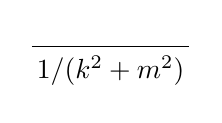
\begin{tikzpicture}
    \draw (0, 0) -- (2, 0) node [pos=0.5, below] {$1/(k^2 + m^2)$} node [pos=0.5, above] { };
  \end{tikzpicture}}\quad\quad
  \makecenter{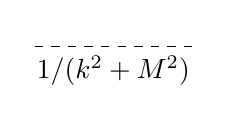
\begin{tikzpicture}
    \draw [dashed] (0, 0) -- (2, 0) node [pos=0.5, below] {$1/(k^2 + M^2)$} node [pos=0.5, above] { };
  \end{tikzpicture}}\quad\quad
  \makecenter{\begin{tikzpicture}[scale=0.707]
    \draw (0, 0) -- (2, 2);
    \draw [dashed] (0, 2) -- (2, 0);
    \node [circ] at (1, 1) {};
    \node [right] at (2, 1) {$-\lambda$};
  \end{tikzpicture}}
\end{center}
As in the case of zero-dimensional QFT, if we are only interested in the correlations involving $x(t)$, then we can integrate out the field $y(t)$ first. The effective potential can be written as
\[
  \int \D y\; \exp\left(-\frac{1}{2} \int_{S^1} y\left(-\frac{\d^2}{\d t^2} + M^2 + \frac{\lambda x^2}{2}\right) y \;\d t\right),
\]
where we integrated by parts to turn $\dot{y}^2$ to $y \ddot{y}$.

We start doing dubious things. Recall that we previously found that for a bilinear operator $M: \R^n \times \R^n \to \R$, we have
\[
  \int_{\R^n} \d^n x\; \exp\left(- \frac{1}{2} M(x, x)\right) = \frac{(2 \pi)^{n/2}}{\sqrt{\det{M}}}.
\]
Now, we can view our previous integral just as a Gaussian integral over the operator
\[
  (y, \tilde{y}) \mapsto \int_{S^1} y\left(-\frac{\d^2}{\d t^2} + M^2 + \frac{\lambda x^2}{2}\right) \tilde{y} \;\d t\tag{$*$}
\]
on the vector space of fields. Thus, (ignoring the factors of $(2\pi)^{n/2}$) we can formally write the integral as
\[
  \det \left(-\frac{\d^2}{\d t^2} + M^2 + \frac{\lambda x^2}{2}\right)^{-1/2}.
\]
$S_{\mathrm{eff}}[x]$ thus looks like
\[
  S_{\mathrm{eff}}[x] = \int_{S^1} \frac{1}{2}(\dot{x}^2 + m^2 x^2) \;\d t + \frac{1}{2} \log \det \left(-\frac{\d^2}{\d t^2} + M^2 + \frac{\lambda x^2}{2}\right)
\]
We now continue with our formal manipulations. Note that $\log \det = \tr \log$, since $\det$ is the product of eigenvalues and $\tr$ is the sum of them. Then if we factor our operators as
\[
  -\frac{\d^2}{\d t^2} + M^2 + \frac{\lambda x^2}{2} = \left(-\frac{\d^2}{\d t^2} + M^2\right)\left(1 - \lambda \left(-\frac{\d^2}{\d t^2} + M^2\right)^{-1} \frac{x^2}{2}\right),
\]
then we can write the last term in the effective potential as
\[
 \frac{1}{2} \tr \log \left(-\frac{\d^2}{\d t^2} + M^2\right) + \frac{1}{2} \tr \log \left(1 - \lambda \left(\frac{\d^2}{\d t^2} - M^2\right)^{-1} \frac{x^2}{2}\right)
\]
The first term is field independent, so we might as well drop it. We now look carefully at the second term. The next dodgy step to take is to realize we know what the inverse of the differential operator
\[
  \frac{\d^2}{\d t^2} - M^2
\]
is. It is just the Green's function! More precisely, it is the convolution with the Green's function. In other words, it is given by the function $G(t, t')$ such that
\[
  \left(\frac{\d^2}{\d t^2} - M^2 \right) G(t, t') = \delta(t - t').
\]
Equivalently, this is the propagator of the $y$ field. If we actually try to solve this, we find that we have
\[
  G(t, t') = \frac{1}{2M} \sum_{n \in \Z} \exp\left(-M \left|t - t' + \frac{k}{T}\right|\right).
\]
We don't actually need this formula. The part that will be important is that it is $\sim \frac{1}{M}$.

We now try to evaluate the effective potential. When we expand
\[
  \log \left(1 - \lambda G(t, t') \frac{x^2}{2}\right),
\]
the first term in the expansion is
\[
  -\lambda G(t, t') \frac{x^2}{2}.
\]
What does it mean to take the trace of this? We pick a basis for the space we are working on, say $\{\delta(t - t_0): t_0 \in S^1\}$. Then the trace is given by
\[
  \int_{t_0 \in S^1} \d t_0\; \int_{t \in S^1}\d t\; \delta(t - t_0) \left(\int_{t' \in S^1} \d t'\; (-\lambda) G(t, t') \frac{x^2(t')}{2} \delta(t' - t_0)\right).
\]
We can dissect this slowly. The rightmost integral is nothing but the definition of how $G$ acts by convolution. Then the next $t$ integral is the definition of how bilinear forms act, as in $(*)$. Finally, the integral over $t_0$ is summing over all basis vectors, which is what gives us the trace. This simplifies rather significantly to
\[
  -\frac{\lambda}{2} \int_{t \in S^1} G(t, t) x^2(t) \;\d t.
\]
In general, we find that we obtain
\begin{multline*}
  \tr \log \left(1 - \lambda G(t, t') \frac{x^2}{2}\right) \\
  = - \frac{\lambda}{2} \int_{S_1}G(t, t) x^2(t) \;\d t - \frac{\lambda^2}{8} \int_{S^1 \times S^1} \d t\; \d t' G(t', t) x^2(t) G(t, t') x^2(t') \cdots
\end{multline*}

These terms in the effective field theory are \emph{non-local}! It involves integrating over many different points in $S^1$. In fact, we should have expected this non-locality from the corresponding Feynman diagrams. The first term corresponds to
\begin{center}
  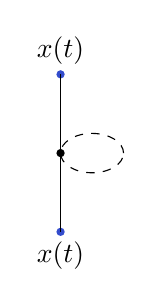
\begin{tikzpicture}
    \node [circ, mblue] at (0, 0) {};
    \node [above] at (0, 0) {$x(t)$};
    \node [circ, mblue] at (0, -2) {};
    \node [below] at (0, -2) {$x(t)$};
    \draw (0, 0) -- (0, -2);

    \node [circ] at (0, -1) {};

    \draw [dashed] (0.4, -1) ellipse (0.4 and 0.25);
  \end{tikzpicture}
\end{center}
Here $G(t, t)$ corresponds to the $y$ field propagator, and the $-\frac{\lambda}{2}$ comes from the vertex.

The second diagram we have looks like this:
\begin{center}
  \begin{tikzpicture}[eqpic]
    \draw (-0.2, 0) node [circ, mblue] {} node [above] {$x(t)$} -- +(0.2, -1) node [circ] {} -- +(0, -2) node [circ, mblue] {} node [below] {$x(t)$};
    \draw (1, 0) node [circ, mblue] {} node [above] {$x(t')$} -- +(-0.2, -1) node [circ] {} -- +(0, -2) node [circ, mblue] {} node [below] {$x(t')$};
    \draw [dashed] (0.4, -1) ellipse (0.4 and 0.25);
  \end{tikzpicture}
\end{center}
We see that the first diagram is local, as there is just one vertex at time $t$. But in the second diagram, we use the propagators to allow the $x$ at time $t$ to talk to $x$ at time $t'$. This is non-local!

Non-locality is generic. Whenever we integrate out our fields, we get non-local terms. But non-locality is terrible in physics. It means that the equations of motion we get, even in the classical limit, are going to be integral differential equations, not just normal differential equations. For a particle to figure out what it should do here, it needs to know what is happening in the far side of the universe!

To make progress, we note that if $M$ is very large, then we would expect $G(t, t')$ could be highly suppressed for $t \not= t'$. So we can try to expand around $t = t'$. Recall that the second term is given by
\[
  \int \d t\; \d t' G(t, t')^2 x^2(t) x^2(t')
\]
We can write out $x'(t^2)$ as
\[
  x'(t^2) = x^2 (t) + 2x(t) \dot{x}(t) (t' - t) + \left(\dot{x}^2(t) + \frac{1}{2} x(t) \dot{x}(t)\right) (t - t')^2 + \cdots.
\]
Using the fact that $G(t, t')$ depends on $t'$ only through $M(t' - t)$, by dimensional analysis, we get an expansion that looks like
\[
  \frac{1}{M^2} \int \d t\; \frac{\alpha}{M} x^4(t) + \frac{\beta}{M^3} \left(x^2 \dot{x}^2 + \frac{1}{2} x^2 \ddot{x}\right) + \frac{\gamma}{M^5} (\text{4-derivative terms}) + \cdots
\]
Here $\alpha, \beta, \gamma$ are dimensionless quantities.

Thus, we know that every extra derivative is accompanied by a further power of $\frac{1}{M}$. Thus, provided $x(t)$ is slowly varying on scales of order $\frac{1}{M}$, we may hope to truncate the series.

Thus, at energies $E \ll M$, our theory looks approximately local. So as long as we only use our low-energy approximation to answer low-energy questions, we are fine. However, if we try to take our low-energy theory and try to extrapolate it to higher and higher energies, up to $E \sim M$, it is going to be nonsense. In particular, it becomes non-unitary, and probability is not preserved.

This makes sense. By truncating the series at the first term, we are ignoring all the higher interactions governed by the $y$ fields. By ignoring them, we are ignoring some events that have non-zero probability of happening, and thus we would expect probability not to be conserved.

There are two famous examples of this. The first is weak interactions. At very low energies, weak interactions are responsible for $\beta$-decay. The effective action contains a quartic interaction
\[
  \int \d^4 x\; \bar\psi_e n \nu_e p \; G_{\mathrm{weak}}.
\]
This coupling constant $G_{\mathrm{weak}}$ has mass dimensional $-1$. At low energies, this is a perfectly well description of beta decay. However, this is suspicious. The fact that we have a coupling constant with negative mass dimension suggests this came from integrating some fields out.

At high energies, we find that this \emph{4-Fermi theory} becomes non-unitary, and $G_{\mathrm{weak}}$ is revealed as an approximation to a $W$-boson propagator. Instead of an interaction that looks like this:
\begin{center}
  \begin{tikzpicture}
    \draw (0, 0) -- (2, 2);
    \draw (0, 2) -- (2, 0);
    \node [circ] at (1, 1) {};
  \end{tikzpicture}
\end{center}
what we really have is
\begin{center}
  \begin{tikzpicture}
    \draw (0, 0) -- (0.75, 1) -- (0, 2);

    \draw [decorate, decoration={snake}](0.75, 1) -- (2.25, 1) node [pos=0.5, above=0.3em] {$W$};
    \draw (3, 2) -- (2.25, 1) -- (3, 0);
    \node [circ] at (0.75, 1) {};
    \node [circ] at (2.25, 1) {};
  \end{tikzpicture}
\end{center}
There are many other theories we can write down that has negative mass dimension, the most famous one being general relativity.

\subsection{Quantum gravity in one dimension}
In quantum gravity, we also include a (path) integral over all metrics on our spacetime, up to diffeomorphism (isometric) invariance. We also sum over all possible topologies of $M$. In $d = 1$ (and $d = 2$ for string theory), we can just do this.

In $d = 1$, a metric $g$ only has one component $g_{tt}(t) = e(t)$. There is no curvature, and the only diffeomorphism invariant of this metric is the total length
\[
  T = \oint e(t) \;\d t.
\]
So the instruction to integrate over all metrics modulo diffeomorphism is just the instruction to integrate over all possible lengths of the worldline $T \in (0, \infty)$, which is easy. Let's look at that.

The path integral is given by
\[
  \int_T \d T \;\int_{C_{[0, T]} [y, x]} \D x\; e^{-S[x]}.
\]
where as usual
\[
  S[x] = \frac{1}{2} \int_0^T \dot{x}^2 \;\d t.
\]
Just for fun, we will include a ``cosmological constant'' term into our action, so that we instead have
\[
  S[x] = \frac{1}{2} \int_0^T \dot{x}^2 + \frac{m^2}{2}\;\d t.
\]
The reason for this will be revealed soon.

We can think of the path integral as the heat kernel, so we can write it as
\begin{align*}
  \int_0^\infty\; \d T\; \brak{y} e^{-HT} \bket{x} &= \int_0^\infty \d T\; \frac{\d^n p\; \d^n q}{ (2\pi)^n} \braket{y}{q} \brak{q} e^{-HT}\bket{p} \braket{p}{x}\\
  &= \int_0^\infty \d T\; \frac{\d^n p\; \d ^n q}{(2\pi)^n} e^{ip\cdot x - i q \cdot y} e^{-T(p^2 + m^2)/2} \delta^n(p - q)\\
  &= \int_0^\infty \d T\; \frac{\d^n p}{(2\pi)^n} e^{ip\cdot (x - y)} e^{-T(p^2 + m^2)/2}\\
  &= 2 \int \frac{\d^n p}{(2\pi)^n} \frac{e^{ip\cdot (x - y)}}{p^2 + m^2}\\
  &= 2 D(x, y),
\end{align*}
where $D(x, y)$ is the propagator for a scalar field on the \emph{target space} $\R^n$ with action
\[
  S[\Phi] = \int \d^n x \; \frac{1}{2} (\partial \Phi)^2 + \frac{m^2}{2} \Phi^2.
\]
So a $1$-dimensional quantum gravity theory with values in $\R^n$ is equivalent to (or at least has deep connections to) a scalar field theory on $\R^n$.

How about interactions? So far, we have been taking rather unexciting 1-dimensional manifolds as our universe, and there are only two possible choices. If we allow singularities in our manifolds, then we would allow \emph{graphs} instead of just a line and a circle. Quantum gravity then says we should not only integrate over all possible lengths, but also all possible graphs.

For example, to compute correlation functions such as $\bra \Phi(x_1) \cdots \Phi(x_n)\ket$ in $\Phi^4$ theory on $\R^n$, say, we consider all $4$-valent with $n$ external legs with one endpoint at each of the $x_i$, and then we proceed just as in quantum gravity.

For example, we get a contribution to $\bra \Phi(x) \Phi(y)\ket$ from the graph
\begin{center}
  \begin{tikzpicture}
    \draw (0, 0) node [circ] {} node [left] {$x$} -- (2, 0) node [circ] {} node [right] {$x$};

    \node [circ] at (1, 0) {};
    \draw (1, 0.4) ellipse (0.2 and 0.4);
  \end{tikzpicture}
\end{center}
The contribution to the quantum gravity expression is
\[
  \int\limits_{\mathclap{z \in \R^n}}\d^n z \int\limits_{\mathclap{[0, \infty)^3}} \d T_1\, \d T_2\, \d T_3\, \int\limits_{\mathclap{\mathcal{C}_{T_1}[z, x]}} \D x\, e^{-S_{T_1}[x]} \int\limits_{\mathclap{C_{T_2}[z, z]}} \D x\, e^{-S_{T_2}[x]} \int\limits_{\mathclap{C_{T_3}[y, z]}} \D x\, e^{-S_{T_3}[x]},
\]
where
\[
  S_T[x] = \frac{1}{2} \int_0^T x^2 \;\d t + \frac{m^2}{2}\int_0^T \d t.
\]
We should think of the second term as the ``cosmological constant'', while the 1D integrals over $T_i$'s are the ``1d quantum gravity'' part of the path integral (also known as the \term{Schwinger parameters} for the graph).

We can write this as
\begin{align*}
  &\hphantom{{}={}} \int \d^n z \; \d T_1 \;\d T_2 \;\d T_3\; \brak{z} e^{-HT_1} \bket{x} \brak{z}e^{-HT_2} \bket{z} \brak{y} e^{-H T_3} \bket{z}.\\
  \intertext{Inserting a complete set of eigenstates between the position states and the time evolution operators, we get}
  &= \int \frac{\d^n p\; \d^n \ell\;\d^n q}{(2\pi)^{3n}} \frac{e^{ip\cdot(x - z)}}{p^2 + m^2} \frac{e^{iq\cdot(y - z)}}{q^2 + m^2} \frac{e^{i\ell\cdot(z - z)}}{\ell^2 + m^2}\\
  &= \int \frac{\d^n p\; \d^n \ell}{(2\pi)^{2n}} \frac{e^{ip\cdot (x - y)}}{(p^2 + m^2)^2} \frac{1}{\ell^2 + m^2}.
\end{align*}
This is exactly what we would have expected if we viewed the above diagram as a Feynman diagram:
\begin{center}
  \begin{tikzpicture}
    \draw (0, 0) node [circ] {} node [left] {$x$} -- (2, 0) node [circ] {} node [right] {$y$};

    \node at (0.5, 0) [below] {$p$};
    \node at (1.5, 0) [below] {$p$};

    \node [circ] at (1, 0) {};
    \draw (1, 0.4) ellipse (0.2 and 0.4);
    \node at (1.2, 0.4) [right] {$\ell$};
  \end{tikzpicture}
\end{center}
This is the \term{worldline perspective} to QFT, and it was indeed Feynman's original approach to doing QFT.

\section{Symmetries of the path integral}
From now on, we will work with quantum field theory in general, and impose no restrictions on the dimension of our universe. The first subject to study is the notion of symmetries.

We first review what we had in classical field theory. In classical field theory, Noether's theorem relates symmetries to conservation laws. For simplicity, we will work with the case of a flat space.

Suppose we had a variation
\[
  \delta \phi = \varepsilon f(\phi, \partial \phi)
\]
of the field. The most common case is when $f(\phi, \partial \phi)$ depends on $\phi$ only locally, in which case we can think of the transformation as being generated by the vector
\[
  V_f = \int_M \d^d x \; f(\phi, \partial \phi) \frac{\delta}{\delta \phi(x)}
\]
acting on the ``space of fields''.

If the function $S[\phi]$ is invariant under $V_f$ when $\varepsilon$ is constant, then for general $\varepsilon(x)$, we must have
\[
  \delta S = \int \d^d x\; j^\mu(x)\; \partial_\mu \varepsilon.
\]
for some field-dependent current $j_\mu(x)$ (we can actually find an explicit expression for $j_\mu$). If we choose $\varepsilon(x)$ to have compact support, then we can write
\[
  \delta S = - \int \d^d x\; (\partial^\mu j_\mu)\;\varepsilon(x).
\]
On \emph{solutions} of the field equation, we know the action is stationary under arbitrary variations. So $\delta S = 0$. Since $\varepsilon(x)$ was arbitrary, we must have
\[
  \partial^\mu j_\mu = 0.
\]
So we know that $j_\mu$ is a \term{conserved current}.

Given any such conserved current, we can define the \term{charge} $Q[N]$ associated to an (oriented) co-dimension $1$ hypersurface $N$ as
\[
  Q[N] = \int_N n^\mu j_\mu\; \d^{d - 1}x,
\]
where $n^\mu$ is the normal vector to $N$. Usually, $N$ is a time slice, and the normal points in the future direction.

Now if $N_0$ and $N_1$ are two such hypersurfaces bounding a region $M' \subseteq M$, then by Stokes' theorem, we have
\[
  Q[N_0] - Q[N_1] = \left(\int_{N_0} - \int_{N_1}\right) n^\mu j_\mu \;\d^{n - 1}x = \int_{M'} (\partial^\mu j_\mu)\;\d^n x = 0.
\]
So we find
\[
  Q[N_0] = Q[N_1].
\]
This is the conservation of charge!

\subsection{Ward identities}
The derivation of Noether's theorem used the classical equation of motion. But in a quantum theory, the equation of motion no longer holds. We must re-examine what happens in the quantum theory.

Suppose a transformation $\phi \mapsto \phi'$ of the fields has the property that
\[
  \D \phi\; e^{-S[\phi]} = \D \phi'\; e^{-S[\phi']}.
\]
In theory, the whole expression $\D \phi\; e^{-S[\phi]}$ is what is important in the quantum theory. In practice, we often look for symmetries where $\D \phi$ and $e^{-S[\phi]}$ are separately conserved. In fact, what we will do is that we look for a symmetry that preserves $S[\phi]$, and then try to find a regularization of $\D \phi$ that is manifestly invariant under the symmetry.

Often, it is \emph{not} the case that the obvious choice of regularization of $\D \phi$ is manifestly invariant under the symmetry. For example, we might have a $S[\phi]$ that is rotationally invariant. However, if we regularize the path integral measure by picking a lattice and sampling $\phi$ on different points, it is rarely the case that this lattice is rotationally invariant.

In general, there are two possibilities:
\begin{enumerate}
  \item The symmetry could be restored in the limit. This typically means there exists a regularized path integral measure manifestly invariant under this symmetry, but we just didn't use it. For example, rotational invariance is not manifestly present in lattice regularization, but it is when we do the cut-off regularization.
  \item It could be that the symmetry is not restored. It is said to be \emph{anomalous}\index{anomalous symmetry}, i.e.\ broken in the quantum theory. In this case, there can be no invariant path integral measure. An example is scale invariance in QED, if the mass of the electron is $0$.
\end{enumerate}
Sometimes, it can be hard to tell. For now, let's just assume we are in a situation where $\D \phi = \D \phi'$ when $\varepsilon$ is constant. Then for any $\varepsilon(x)$, we clearly have
\[
  \mathcal{Z} = \int \D \phi\; e^{-S [\phi]} = \int \D \phi' e^{-S[\phi']},
\]
since this is just renaming of variables. But using the fact that the measure is invariant when $\varepsilon$ is constant, we can can expand the right-hand integral in $\varepsilon$, and again argue that it must be of the form
\[
  \int \D \phi'\; e^{-S[\phi']} = \int \D \phi\; e^{-S[\phi]} \left(1 - \int_M j_\mu \partial^\mu \varepsilon\; \d^n x\right).
\]
in first order in $\varepsilon$. Note that in general, $j_\mu$ can receive contributions from $S[\phi]$ and $\D \phi$. But if it doesn't receive any contribution from $\D \phi$, then it would just be the classical current.

Using this expansion, we deduce that we must have
\[
  \int \D \phi \; e^{-S[\phi]} \int_M j_\mu \partial^\mu \varepsilon \;\d^d x = 0.
\]
Integrating by parts, and using the definition of the expectation, we can write this as
\[
  -\int_M \varepsilon \partial^\mu \bra j_\mu (x)\ket\; \d^n x,
\]
for any $\varepsilon$ with compact support. Note that we dropped a normalization factor of $\mathcal{Z}$ in the definition of $\bra j_\mu(x)\ket$, because $\mathcal{Z}$ times zero is still zero. So we know that $\bra j_\mu (x)\ket$ is a conserved current, just as we had classically.

\subsubsection*{Symmetries of correlation functions}
Having a current is nice, but we want to say something about actual observable quantities, i.e.\ we want to look at how how symmetries manifest themselves with correlation functions. Let's look at what we might expect. For example, if our theory is translation invariant, we might expect, say
\[
  \bra \phi(x) \phi(y)\ket = \bra \phi(x - a) \phi(y - a)\ket
\]
for any $a$. This is indeed the case.

Suppose we have an operator $\mathcal{O}(\phi)$. Then under a transformation $\phi \mapsto \phi'$, our operator transforms as
\[
  \mathcal{O}(\phi) \mapsto \mathcal{O}(\phi'),
\]
By definition, the correlation function is defined by
\[
  \bra \mathcal{O}(\phi)\ket = \frac{1}{\mathcal{Z}} \int \D \phi\;e^{-S[\phi]} \mathcal{O}(\phi).
\]
Note that despite the appearance of $\phi$ on the left, it is not a free variable. For example, the correlation $\bra \phi(x_1) \phi(x_2)\ket$ is not a function of $\phi$.

We suppose the transformation $\phi \mapsto \phi'$ is a symmetry. By a trivial renaming of variables, we have
\begin{align*}
  \bra \mathcal{O}(\phi)\ket &= \frac{1}{\mathcal{Z}} \int \D \phi'\; e^{-S[\phi']} \mathcal{O} (\phi')\\
  \intertext{By assumption, the function $\D \phi\;e^{-S[\phi]}$ is invariant under the transformation. So this is equal to}
  &= \frac{1}{\mathcal{Z}} \int \D \phi\; e^{-S[\phi]} \mathcal{O}(\phi')\\
  &= \bra \mathcal{O}(\phi')\ket.
\end{align*}
This is, of course, not surprising. To make this slightly more concrete, we look at an example.

%Now we further suppose this transformation is a symmetry. By definition, we can write
%\[
% \bra \mathcal{O}_1(x_1) \cdots \mathcal{O}_n(x_n)\ket = \frac{1}{\mathcal{Z}} \int \D \phi e^{-S[\phi]} \mathcal{O}_1(\phi(x_1)) \cdots \mathcal{O}_n(\phi(x_n)).
%\]
%Trivially, by renaming of variables, this is equal to
%\[
% \frac{1}{\mathcal{Z}} \int \D \phi' e^{-S[\phi']} \mathcal{O}_1(\phi'(x_1)) \cdots \mathcal{O}_n(\phi'(x_n)).
%\]
%Using the invariance of the measure, this is equal to
%\[
% \frac{1}{\mathcal{Z}} \int \D \phi\;e^{-S[\phi]} \mathcal{O}_1(\phi'(x_1) \cdots \mathcal{O}_n (\phi'(x_n)).
%\]
%Consequently, we find
%\[
% \bra \mathcal{O}_1(\phi(x_n)) \cdots \mathcal{O}_n(\phi(x_n))\ket = \bra \mathcal{O}_1(\phi'(x_n)) \cdots \mathcal{O}_n(\phi'(x_n))\ket.
%\]
%So the correlation function of the original and transformed operators are the agree \emph{in the same theory}.

\begin{eg}
  Consider $(M, g) = (\R^4, \delta)$, and consider spacial translation $x \mapsto x' = x - a$ for a constant vector $a$. A scalar field $\phi$ transforms as
  \[
    \phi(x) \mapsto \phi'(x) = \phi(x - a).
  \]
  In most cases, this is a symmetry.

  We suppose $\mathcal{O}(\phi)$ can be written as
  \[
    \mathcal{O}(\phi) = \mathcal{O}_1(\phi(x_1)) \cdots \mathcal{O}_n(\phi(x_n)),
  \]
  where $\mathcal{O}_i$ depends only on the value of $\phi$ at $x_i$. A canonical example is when $\mathcal{O}(\phi) = \phi(x_1) \cdots \phi(x_n)$ is an $n$-point correlation function.

  Then the above result tells us that
  \[
     \bra \mathcal{O}_1(\phi(x_1)) \cdots \mathcal{O}_n(\phi(x_n))\ket = \bra \mathcal{O}_1(\phi(x_1 - a)) \cdots \mathcal{O}_n(\phi(x_n - a))\ket
  \]
  So the correlation depends only on the separations $x_i - x_j$. We can obtain similar results if the action and measure are rotationally or Lorentz invariant.
% So the scalar operators transform as $\mathcal{O}(\phi(x)) \mapsto \mathcal{O}(\phi(x - a))$. In shorthand, we write $\mathcal{O}(x) \mapsto \mathcal{O}(x - a)$.
%
% Thus, we find that.
% \[
% \bra \mathcal{O}_1(x_1) \cdots \mathcal{O}_n(x_n)\ket = \bra \mathcal{O}_1(x_1 - a) \cdots \mathcal{O}_n(x_n - a)\ket.
% \]
% Hence, the correlation function must depend only on the separation $x_{ij} = x_i - x_j$. Similarly, if the action and measure are rotationally or Lorentz invariant, then under a transformation $L$, we find
% \[
% \bra \mathcal{O}(x_1) \cdots \mathcal{O}_n(x_n)\ket = \bra \mathcal{O}_1(L x_1) \cdots \mathcal{O}_n (L x_n)\ket.
% \]
% So the correlation only depends on the Lorentz invariant separations $x_{ij}^2$.
\end{eg}

\begin{eg}
  Suppose we have a complex field $\phi$, and we have a transformation $\phi \mapsto \phi' = e^{i\alpha}\phi$ for some constant $\alpha \in \R/2\pi \Z$. Then the conjugate field transforms as
  \[
    \bar\phi \mapsto \bar\phi' = e^{-i\alpha} \bar\phi.
  \]
  Suppose this transformation preserves the action and measure. For example, the measure will be preserved if we integrate over the same number of $\phi$ and $\bar\phi$ modes. Consider the operators
  \[
    \mathcal{O}_i (\phi, \bar\phi) = \phi(x_i)^{s_i} \bar\phi(x_i)^{r_i}.
  \]
  Then the operators transform as
  \[
    \mathcal{O}_i(\phi, \bar\phi) \mapsto \mathcal{O}_i (\phi', \bar\phi') = e^{-\alpha (r_i - s_i)} \mathcal{O}_i(\phi, \bar\phi).
  \]
  So symmetry entails
  \[
    \left\bra \prod_{i = 1}^m \mathcal{O}_i(x_i)\right\ket = \exp\left(i \alpha \sum_{i = 1}^m (r_i - s_i)\right) \left\bra \prod_{i = 1}^m \mathcal{O}_i(x_i)\right\ket.
  \]
  Since this is true for all $\alpha$, the correlator must vanish unless
  \[
    \sum_{i = 1}^m r_i = \sum_{i = 1}^m s_i.
  \]
  So we need the same number of $\phi$ and $\bar\phi$ insertions in total.

  We can interpret this in terms of Feynman diagrams --- each propagator joins up a $\phi$ and $\bar\phi$. So if we don't have equal number of $\phi$ and $\bar\phi$, then we can't draw any Feynman diagrams at all! So the correlator must vanish.
\end{eg}

%\begin{eg}
% Consider $(M, g) = (\R^4, \delta)$, and consider spacial translation $x \mapsto x' = x - a$ for a constant vector $a$. A scalar field $\phi$ transforms as
% \[
% \phi(x) \mapsto \phi'(x) = \phi(x - a).
% \]
% In most cases, this is a symmetry. So the scalar operators transform as $\mathcal{O}(\phi(x)) \mapsto \mathcal{O}(\phi(x - a))$. In shorthand, we write $\mathcal{O}(x) \mapsto \mathcal{O}(x - a)$.
%
% Thus, we find that.
% \[
% \bra \mathcal{O}_1(x_1) \cdots \mathcal{O}_n(x_n)\ket = \bra \mathcal{O}_1(x_1 - a) \cdots \mathcal{O}_n(x_n - a)\ket.
% \]
% Hence, the correlation function must depend only on the separation $x_{ij} = x_i - x_j$. Similarly, if the action and measure are rotationally or Lorentz invariant, then under a transformation $L$, we find
% \[
% \bra \mathcal{O}(x_1) \cdots \mathcal{O}_n(x_n)\ket = \bra \mathcal{O}_1(L x_1) \cdots \mathcal{O}_n (L x_n)\ket.
% \]
% So the correlation only depends on the Lorentz invariant separations $x_{ij}^2$.
%\end{eg}

\subsubsection*{Ward identity for correlators}
What we've done with correlators was rather expected, and in some sense trivial. Let's try to do something more interesting.

Again, consider an operator that depends only on the value of $\phi$ at finitely many points, say
\[
  \mathcal{O}(\phi) = \mathcal{O}_1(\phi(x_1)) \cdots \mathcal{O}_n(\phi(x_n)).
\]
As before, we will write the operators as $\mathcal{O}_i(x_i)$ when there is no confusion.

As in the derivation of Noether's theorem, suppose we have an infinitesimal transformation, with $\phi \mapsto \phi + \varepsilon \delta \phi$ that is a symmetry when $\varepsilon$ is constant. Then for general $\varepsilon(x)$, we have
\begin{align*}
  &\hphantom{={}} \int \D \phi\; e^{-S[\phi]} \mathcal{O}_1(\phi(x_1)) \cdots \mathcal{O}_n(\phi(x_n)) \\
  &= \int \D \phi'\; e^{-S[\phi']} \mathcal{O}_1(\phi'(x_1)) \cdots \mathcal{O}_n(\phi'(x_n))\\
  &= \int \D \phi\; e^{-S[\phi]} \left(1 - \int j^\mu (x) \partial_\mu \varepsilon(x) \;\d x\right)\left(\mathcal{O}_1(\phi(x_1)) \cdots \mathcal{O}_n(\phi(x_n))\vphantom{ + \sum_{i = 1}^n \varepsilon(x_i) \delta \mathcal{O}(x_i) \prod_{j \not= i} \mathcal{O}_j(x_j)}\right.\\
  &\hphantom{= \int \D \phi e^{-S[\phi]} \left(1 - \int j^\mu (x) \partial_\mu \varepsilon(x) \;\d x\right)}\left.+ \sum_{i = 1}^n \varepsilon(x_i) \delta \mathcal{O}_i(x_i) \prod_{j \not= i} \mathcal{O}_j(x_j)\right),
\end{align*}
where
\[
  \delta \mathcal{O}(x_i) = \frac{\partial \mathcal{O}}{\partial \phi} \delta \phi.
\]
Again, the zeroth order piece of the correlation function cancels, and to lowest non-trivial order, we find that we must have
\[
   \int \partial^\mu \varepsilon(x) \left\bra j_\mu(x) \prod_{i = 1}^n \mathcal{O}_i(x_i)\right\ket\;\d^d x = \sum_{i = 1}^m \varepsilon(x_i) \left\bra \delta \mathcal{O}_i(x_i) \prod_{j \not= i} \mathcal{O}_j(x_j)\right\ket.
\]
On the left, we can again integrate by parts to shift the derivative to the current term. On the right, we want to write it in the form $\int \varepsilon(x) \cdots \;\d^d x$, so that we can get rid of the $\varepsilon$ term. To do so, we introduce some $\delta$-functions. Then we obtain
\begin{multline*}
  \int \varepsilon(x) \partial^\mu \left\bra j_\mu(x) \prod_{i = 1}^n \mathcal{O}_i(x_i)\right\ket\;\d^d x \\
  = - \sum_{i = 1}^m \int \varepsilon(x) \delta^d(x - x_i) \left\bra \delta \mathcal{O}_i(x_i) \prod_{j \not= i} \mathcal{O}_j(x_j)\right\ket \;\d^d x.
\end{multline*}
Since this holds for arbitrary $\varepsilon(x)$ (with compact support), we must have
\[
  \partial^\mu \left\bra j_\mu (x) \prod \mathcal{O}_i(x_i)\right\ket = -\sum_{i = 1}^n \delta^d(x - x_i)\left\bra \delta \mathcal{O}_i(x_i) \prod_{j \not= i} \mathcal{O}_j(x_j)\right\ket.
\]
This is the \term{Ward identity} for correlation functions. It says that the vector field
\[
  f_\mu (x, x_i) = \left\bra j_\mu (x) \prod_i \mathcal{O}_i (x_i)\right\ket
\]
is divergence free except at the insertions $x_i$.

This allows us to recover the previous invariance of correlations. Suppose $M$ is compact without boundary. We then integrate the Ward identity over all $M$. By Stokes' theorem, we know the integral of any divergence term vanishes. So we obtain
\[
  0 = \int_M \partial^\mu f_\mu(x, x_i)\;\d^d x = -\sum_{i = 1}^n \left\bra \delta \mathcal{O}_i(x_i) \prod_{j \not= i} \mathcal{O}_j(x_j)\right\ket = \delta \left\bra \prod_{i = 1}^n \mathcal{O}_i(x_i)\right\ket,
\]
Of course, this is what we would obtain if we set $\varepsilon(x) \equiv 1$ above.

That was nothing new, but suppose $M' \subseteq M$ is a region with boundary $N_1 - N_0$.
\begin{center}
  \begin{tikzpicture}
    \draw [thick, mblue] (0, 0) -- (2, 2) -- (4, 0) -- (2, -2) -- cycle;

    \draw (0, 0) edge [mred, thick, bend left, fill=morange, fill opacity=0.3] (4, 0);
    \draw (0, 0) edge [mred, thick, bend right, fill=morange, fill opacity=0.3] (4, 0);
    \node at (2, 0.6) [above] {$N_1$};
    \node at (2, -0.6) [below] {$N_0$};
    \node at (2, 0) {$M'$};
  \end{tikzpicture}
\end{center}
Let's see what integrating the Ward identity over $M'$ gives us. The left hand side gives us
\begin{align*}
  \int_{M'} \partial^\mu \left\bra j_\mu (x) \prod_{i = 1}^n \mathcal{O}_i(x_i)\right\ket \;\d^d x &= \int_{N_1 - N_0} n^\mu\left\bra j_\mu (x) \prod_{i = 1}^n \mathcal{O}_i(x_i)\right\ket\;\d^{d - 1}x\\
  &= \left\bra Q[N_1] \prod_{i = 1}^n \mathcal{O}_i(x_i)\right\ket - \left\bra Q[N_0] \prod_{i = 1}^n \mathcal{O}_i(x_i)\right\ket
\end{align*}
The right hand side of Ward's identity just gives us the sum over all points inside $M'$.
\[
  \left\bra Q[N_1] \prod_{i = 1}^n \mathcal{O}_i(x_i)\right\ket - \left\bra Q[N_0] \prod_{i = 1}^n \mathcal{O}_i(x_i)\right\ket = - \sum_{x_i \in M'} \left\bra \delta \mathcal{O}_i(x_i) \prod_{j \not= i}^m \mathcal{O}_j(x_j)\right\ket.
\]
In particular, if $M'$ contains only one point, say $x_1$, and we choose the region to be infinitesimally thin, then in the canonical picture, we have
\[
  \brak{\Omega}\mathcal{T} [\hat{Q}, \hat{\mathcal{O}}_1(x_1)] \prod_{j = 2}^m \hat{\mathcal{O}}_j (x_j)\bket{\Omega} = - \brak{\Omega} \mathcal{T} \left\{\delta \hat{\mathcal{O}}_1 \prod_{j = 2}^n \hat{\mathcal{O}}_j(x_j)\right\}\bket{\Omega},
\]
where $\bket{\Omega}$ is some (vacuum) state. So in the canonical picture, we find that
\[
  \delta \hat{\mathcal{O}} = -[\hat{Q}, \hat{\mathcal{O}}].
\]
So we see that the change of $\hat{\mathcal{O}}$ under some transformation is given by the commutator with the charge operator.

\subsection{The Ward--Takahashi identity}
We focus on an important example of this. The QED action is given by
\[
  S[A, \psi] = \int \d^d x\; \left(\frac{1}{4} F_{\mu\nu}F^{\mu\nu} + i \bar\psi \slashed\D \psi + m \bar\psi \psi\right).
\]
This is invariant under the global transformations
\[
  \psi (x) \mapsto e^{i\alpha} \psi(x),\quad A_\mu(x) \mapsto A_\mu(x)
\]
for constant $\alpha \in \R/2\pi \Z$. The path integral measure is also invariant under this transformation provided we integrate over equal numbers of $\psi$ and $\bar\psi$ modes in the regularization.

In this case, the \emph{classical} current is given by
\[
  j^\mu (x) = \bar\psi (x) \gamma^\mu \psi(x).
\]
We will assume that $\D \psi \D \bar{\psi}$ is invariant under a position-dependent $\alpha$. This is a reasonable assumption to make, if we want our measure to be gauge invariant. In this case, the classical current is also the quantum current.

Noting that the infinitesimal change in $\psi$ is just (proportional to) $\psi$ itself, the Ward identity applied to $\bra\psi(x_1) \bar\psi(x_2)\ket$ gives
\[
  \partial^\mu \bra j_\mu(x) \psi(x_1) \bar\psi(x_2)\ket = - \delta^4(x - x_1) \bra \psi(x_1) \bar\psi(x_2)\ket + \delta^4(x - x_2) \bra \psi(x_1) \bar\psi(x_2)\ket.
\]
We now try to understand what these individual terms mean. We first understand the correlators $\bra \psi(x_1) \bar\psi(x_2)\ket$.

Recall that when we did perturbation theory, the propagator was defined as the Fourier transform of the \emph{free theory} correlator $\bra \psi(x_1) \bar\psi(x_2)\ket$. This is given by
\begin{align*}
  D(k_1, k_2) &= \int \d^4 x_1 \; \d^4 x_2\; e^{ik_1 \cdot x_1} e^{-ik_2 \cdot x_2} \bra \psi(x_1) \bar\psi(x_2)\ket\\
  &= \int \d^4 y \;\d^4 x_2\; e^{i(k_1 - k_2) \cdot x_2} e^{ik_1 \cdot y} \bra \psi(y) \bar\psi(0)\ket\\
  &= \delta^4(k_1 - k_2) \int \d^4 y\; e^{ik\cdot y} \bra \psi(y) \bar\psi(0)\ket.
\end{align*}

Thus, we can interpret the interacting correlator $\bra \psi(x_1) \bar\psi(x_2)\ket$ as the propagator with ``quantum corrections'' due to the interacting field.
\begin{defi}[Exact propagator]\index{exact propagator}
  The \emph{exact (electron) propagator} is defined by
  \[
    S(k) = \int \d^4 y\; e^{ik\cdot y} \bra \psi(y) \bar\psi(0)\ket,
  \]
  evaluated in the full, interacting theory.
\end{defi}

Usually, we don't want to evaluate this directly. Just as we can compute the sum over \emph{all} diagrams by computing the sum over all connected diagrams, then take $\exp$, in this case, one useful notion is a \emph{one-particle irreducible graph}.

\begin{defi}[One-particle irreducible graph]\index{one-particle irreducible graph}\index{1PI}
  A \emph{one-particle irreducible graph} for $\bra \psi \bar\psi\ket$ is a connected Feynman diagram (in momentum space) with two external vertices $\bar\psi$ and $\psi$ such that the graph cannot be disconnected by the removal of one internal line.
\end{defi}
This definition is rather abstract, but we can look at some examples to see what this actually means.
\begin{eg}
  The following are one-particle irreducible graphs:
  \begin{center}
    \begin{tikzpicture}
      \draw [white, decorate, decoration={snake}] (0.8, 0) arc(180:360:0.7) node [pos=0.5, above=0.5em] {$\gamma$};
      \draw (0, 0) node [circ] {} node [above] {$\bar\psi$} -- (3, 0) node [circ] {} node [above] {$\psi$};
      \draw [decorate, decoration={snake}] (0.8, 0) arc(180:0:0.7) node [pos=0.5, above=0.5em] {$\gamma$};
    \end{tikzpicture}
    \begin{tikzpicture}
      \draw (0, 0) node [circ] {} node [above] {$\bar\psi$} -- (3, 0) node [circ] {} node [above] {$\psi$};
      \draw [decorate, decoration={snake}] (0.5, 0) arc(180:0:0.7);
      \draw [decorate, decoration={snake}] (1.2, 0) arc(180:360:0.7);
    \end{tikzpicture}
  \end{center}
  while the following is not:
  \begin{center}
    \begin{tikzpicture}
      \draw (0, 0) node [circ] {} node [above] {$\bar\psi$} -- (4.7, 0) node [circ] {} node [above] {$\psi$};
      \draw [decorate, decoration={snake}] (0.5, 0) arc(180:0:0.7);
      \draw [decorate, decoration={snake}] (2.8, 0) arc(180:0:0.7);
    \end{tikzpicture}
  \end{center}
\end{eg}

We will write
\[
  \begin{tikzpicture}[eqpic]
    \draw [fill=white] (1, 0) circle [radius=0.3] node {1PI};
  \end{tikzpicture}
  =
  \Sigma(\slashed{k})
\]
for the sum of all contributions due to one-particle irreducible graphs. This is known as the \term{electron self-energy}\index{self-energy!electron}. Note that we do not include the contributions of the propagators connecting us to the external legs. It is not difficult to see that any Feynman diagram with external vertices $\bar\psi$, $\psi$ is just a bunch of 1PI's joined together. Thus, we can expand
\[\arraycolsep=0.25em\def\arraystretch{2.2}
  \begin{array}{ccccc}
  S(k) & \sim &
  \begin{tikzpicture}[eqpic]

    \draw [fill, white] (0.7, 0.3) rectangle (1.3, -0.3);
    \draw (0, 0) node [circ] {} node [above] {$\bar\psi$} -- (2, 0) node [circ] {} node [above] {$\psi$};
    \draw [opacity=0] (0, 0) node [circ] {} node [below] {$\bar\psi$} -- (2, 0) node [circ] {} node [below] {$\psi$};
  \end{tikzpicture}
  &+&
  \begin{tikzpicture}[eqpic]
    \draw (0, 0) node [circ] {} node [above] {$\bar\psi$} -- (2, 0) node [circ] {} node [above] {$\psi$};
    \draw [opacity=0] (0, 0) node [circ] {} node [below] {$\bar\psi$} -- (2, 0) node [circ] {} node [below] {$\psi$};

    \draw [fill] (0.7, 0.3) rectangle (1.3, -0.3);
  \end{tikzpicture}\\
  & & \displaystyle\frac{1}{i \slashed{k} + m} &+& \text{quantum corrections}.
\end{array}
\]
with the quantum corrections given by
\[
  \begin{tikzpicture}[eqpic]
    \draw (0, 0) node [circ] {} node [above] {$\bar\psi$} -- (2, 0) node [circ] {} node [above] {$\psi$};

    \draw [fill] (0.7, 0.3) rectangle (1.3, -0.3);
    \draw [opacity=0] (0, 0) node [circ] {} node [below] {$\bar\psi$} -- (2, 0) node [circ] {} node [below] {$\psi$};
  \end{tikzpicture}
  =
  \begin{tikzpicture}[eqpic]
    \draw (0, 0) node [circ] {} node [above] {$\bar\psi$} -- (2, 0) node [circ] {} node [above] {$\psi$};

    \draw [fill=white] (1, 0) circle [radius=0.3] node {1PI};
    \draw [opacity=0] (0, 0) node [circ] {} node [below] {$\bar\psi$} -- (2, 0) node [circ] {} node [below] {$\psi$};
  \end{tikzpicture}
  +
  \begin{tikzpicture}[eqpic]
    \draw (0, 0) node [circ] {} node [above] {$\bar\psi$} -- (3, 0) node [circ] {} node [above] {$\psi$};

    \draw [fill=white] (1, 0) circle [radius=0.3] node {1PI};
    \draw [fill=white] (2, 0) circle [radius=0.3] node {1PI};
    \draw [opacity=0] (0, 0) node [circ] {} node [below] {$\bar\psi$} -- (3, 0) node [circ] {} node [below] {$\psi$};
  \end{tikzpicture}
  + \cdots
\]
This sum is easy to perform. The diagram with $n$ many 1PI's has contributions from $n$ many 1PI's and $n + 1$ many propagators. Also, momentum contribution forces them to all have the same momentum. So we simply have a geometric series
\begin{align*}
  S(k) &\sim \frac{1}{i\slashed{k} + m} + \frac{1}{i\slashed{k} + m} \Sigma(\slashed{k}) \frac{1}{i\slashed{k} + m} + \frac{1}{i\slashed{k} + m} \Sigma(\slashed{k}) \frac{1}{i\slashed{k} + m} \Sigma(\slashed{k}) \frac{1}{i\slashed{k} + m} + \cdots\\
  &= \frac{1}{i\slashed{k} + m- \Sigma(\slashed{k})}.
\end{align*}

We can interpret this result as saying integrating out the virtual photons gives us a shift in the kinetic term by $\Sigma(\slashed{k})$.

We now move on to study the other term. It was the expectation
\[
  \bra j_\mu(x) \psi(x_1) \bar\psi(x_2)\ket.
\]
We note that using the definition of $\D$, our classical action can be written as
\[
  S[A, \psi] = \int \d^d x\; \frac{1}{4} F_{\mu\nu}F^{\mu\nu} + \bar\psi \slashed \partial \psi + j^\mu A_\mu + m \bar\psi \psi.
\]
In position space, this gives interaction vertices of the form
\begin{center}
  \begin{tikzpicture}
    \node [circ] at (0, 0) {};
    \node [circ] at (1.5, -0.5) {};
    \node [circ] at (3, 0) {};
    \node [above] at (0, 0) {$x_1$};
    \node [above] at (1.5, -0.5) {$x$};
    \node [above] at (3, 0) {$x_2$};

    \draw [/tikzfeynman/fermion] (0, 0) -- (1.5, -0.5);
    \draw [/tikzfeynman/fermion] (1.5, -0.5) -- (3, 0);
    \draw [/tikzfeynman/photon] (1.5, -0.5) -- (1.5, -2);
  \end{tikzpicture}
\end{center}
Again, we want to consider quantum corrections to this interaction vertex. It turns out the interesting correlation function is exactly $\bra j_\mu(x) \psi(x_1) \bar\psi(x_2)\ket$.

This might seem a bit odd. Why do we not just look at the vertex itself, and just consider $\bra j_\mu\ket$? Looking at $\psi j_\mu \bar\psi$ instead corresponds to including including the propagators coming from the external legs. The point is that there can be photons that stretch \emph{across} the vertex, looking like
\begin{center}
  \begin{tikzpicture}
    \node [circ] at (0, 0) {};
    \node [circ] at (1.5, -0.5) {};
    \node [circ] at (3, 0) {};
    \node [above] at (0, 0) {$x_1$};
    \node [above] at (1.5, -0.5) {$x$};
    \node [above] at (3, 0) {$x_2$};

    \draw [/tikzfeynman/fermion] (0, 0) -- (1.5, -0.5);
    \draw [/tikzfeynman/fermion] (1.5, -0.5) -- (3, 0);
    \draw [/tikzfeynman/photon] (1.5, -0.5) -- (1.5, -2);
    \draw (0.75, -0.25) edge [bend left, /tikzfeynman/photon] (2.25, -0.25);
  \end{tikzpicture}
\end{center}
So when doing computations, we must involve the two external electron propagators as well. (We do not include the photon propagator. We explore what happens when we do that in the example sheet)

We again take the Fourier transform of the correlator, and define
\begin{defi}[Exact electromagnetic vertex]\index{exact electromagnetic vertex}
  The \emph{exact electromagnetic vertex} $\Gamma_\mu(k_1, k_2)$ is defined by
  \begin{multline*}
   \delta^4(p + k_1 - k_2) S(k_1) \Gamma_\mu(k_1, k_2) S(k_2) \\
   = \int \d^4 x\; \d^4 x_1\; \d^4 x_2\; \bra j_\mu(x) \psi(x_1) \bar\psi(x_2)\ket e^{ip\cdot x} e^{ik_1 \cdot x_1} e^{-ik_2 \cdot x_2}.
 \end{multline*}
\end{defi}
Note that we divided out the $S(k_1)$ and $S(k_2)$ in the definition of $\Gamma_\mu(k_1, k_2)$, because ultimately, we are really just interested in the vertex itself.

Can we figure out what this $\Gamma$ is? Up to first order, we have
\[
  \bra \psi(x_1) j_\mu(x) \bar\psi(x_2)\ket \sim \bra \psi(x_1) \bar\psi(x)\ket \gamma_\mu \bra \psi(x) \bar\psi(x_2)\ket + \text{quantum corrections}.
\]
So in momentum space, after dividing out by the exact propagators, we obtain
\[
  \Gamma_\mu(k_1, k_2) = \gamma_\mu + \text{quantum corrections}.
\]
This first order term corresponds to diagrams that do \emph{not} include photons going across the two propagators, and just corresponds to the classical $\gamma_\mu$ inside the definition of $j_\mu$. The quantum corrections are the interesting parts.

In the case of the exact electron propagator, we had this clever idea of one-particle irreducible graphs that allowed us to simplify the propagator computations. Do we have a similar clever idea here? Unfortunately, we don't. But we don't have to! The Ward identity relates the exact vertex to the exact electron propagator.

Taking the Fourier transform of the Ward identity, and dropping some $\delta$-functions, we obtain
\[
  (k_1 - k_2)_\mu S(k_1) \Gamma^\mu (k_1, k_2) S(k_2) = i S(k_1) - i S(k_2).
\]
Recall that $S(k_i)$ are matrices in spinor space, and we wrote them as $\frac{1}{\cdots}$. So it is easy to invert them, and we find
\begin{align*}
  (k_1 - k_2)_\mu \Gamma^\mu(k_1, k_2) &= i S^{-1}(k_2) - i S^{-1}(k_1)\\
  &= -i (i \slashed{k}_1 + m - \Sigma(\slashed{k}_1) - i \slashed{k}_2 - m + \Sigma(\slashed{k}_2))\\
  &= (k_1 - k_2)_\mu \gamma^\mu + i (\Sigma(\slashed{k}_1) - \Sigma(\slashed{k}_2)).
\end{align*}
This gives us an explicit expression for the quantum corrections of the exact vertex $\Gamma^\mu$ in terms of the quantum corrections of the exact propagator $S(k)$.

Note that very little of this calculation relied on what field we actually worked with. We could have included more fields in the theory, and everything would still go through. We might obtain a different value of $\Sigma(\slashed{k})$, but this relation between the quantum corrections of $\Gamma^\mu$ and the quantum corrections of $S$ still holds.

What is the ``philosophical'' meaning of this? Recall that the contributions to the propagator comes from the $\bar\psi \slashed{\partial} \psi$ term, while the contributions to the vertex comes from the $\bar\psi \slashed{A} \psi$ term. The fact that their quantum corrections are correlated in such a simple way suggests that our quantum theory treats the $\bar\psi \slashed{D} \psi$ term as a whole, and so they receive the ``same'' quantum corrections. In other words, the quantum theory respects gauge transformations. When we first studied QED, we didn't understand renormalization very well, and the Ward identity provided a sanity check that we didn't mess up the gauge invariance of our theory when regularizing.

How could we have messed up? In the derivations, there was one crucial assumption we made, namely that $\D \psi \D \bar\psi$ is invariant under \emph{position-dependent} transformations $\psi(x) \mapsto e^{i\alpha(x)} \psi(x)$. This was needed for $j_\mu$ to be the classical current. This is true if we regularized by sampling our field at different points in space, as long as we included the same number of $\psi$ and $\bar\psi$ terms.

However, historically, this is not what we used. Instead, we imposed cutoffs in the Fourier modes, asking $k^2 \leq \Lambda_0$. This is \emph{not} compatible with arbitrary changes $\psi(x) \mapsto e^{i\alpha(x)} \psi(x)$, as we can introduce some really high frequency changes in $\psi$ by picking a wild $\alpha$.


%\separator
%We now want to look at the other quantity $\bra \psi(x_1) j_\mu(x) \bar\psi(x_2)\ket$ in the Ward identity. This corresponds to the Feynman graphs that connect electron field insertions at $x_1, x_2$ to the current at $x$.
%
%We define the \term{exact electromagnetic vertex} $\Gamma_\mu(k_1, k_2)$ by
%\begin{align*}
% &\hphantom{={}}\int \d^4 x\; \d^4 x_1\; \d^4 x_2\; \bra j_\mu(x) \psi(x_1) \bar\psi(x_2)\ket e^{ip\cdot x} e^{ik_1 \cdot x_1} e^{-ik_2 \cdot x_2}\\
% &= \int \d^4 x\; \d^4 x_1\; \d^4 x_2\; \bra j_\mu (x - x_2) \psi(x_1 - x_2) \bar\psi(0) \ket\\
% &\hphantom{\int \d^4 x\; \d^4 x_1\; \d^4 x_2\; hereissomespacefi} e^{ip\cdot (x - x_2)} e^{ik_1 \cdot (x_1 - x_2)} e^{i(p + k_1 - k_2)\cdot x_2}\\
% &= \delta^4(p + k_1 - k_2) S(k_1) \Gamma_\mu(k_1, k_2) S(k_2),
%\end{align*}
%where $S$ is what we had before, the exact electron propagator. To understand why we write it in this form, note that since
%\[
% j_\mu(x) = \bar\psi(x) \gamma_\mu \psi(x),
%\]
%we know that the quantity
%\[
% \bra \psi(x_1) j_\mu(x) \bar\psi(x_2)\ket
%\]
%contains diagrams coming from
%\[
% \bra \psi(x_1) \bar\psi(x)\ket \gamma_\mu \bra \psi(x) \bar\psi(x_2)\ket
%\]
%Once we Fourier transform this, we just get $S(k_1) \gamma_\mu S(k_2)$. This term corresponds to things of the form
%\begin{center}
% \begin{tikzpicture}
% \draw (0, 0) node [circ] {} node [above] {$\psi(x_1)$} -- (1.5, 0) node [circ] {} node [above] {$\bar\psi(x)$};
% \node at (2, 0) {$\gamma_\mu$};
%
% \draw (2.5, 0) node [circ] {} node [above] {$\psi(x)$} -- (4, 0) node [circ] {} node [above] {$\bar\psi(x_2)$};
% \end{tikzpicture}
%\end{center}
%This is the really boring term. It counts the contributions when virtual interactions happen to the electron from $x_1$ to $x$ ($S(k_1)$), then it meets the current ($\gamma^\mu$), and then as it goes back to $x_2$, some virtual interactions happen again ($S(k_2)$).
%
%The interesting terms are those that come from interactions that happen \emph{across} the electromagnetic vertex, such as
%\begin{center}
% \begin{tikzpicture}
% \draw (-2, 0) node [circ] {} node [above] {$\psi(x_1)$} -- (-0.25, 0) node [circ] {};
%
% \draw (0.25, 0) node [circ] {} -- (2, 0) node [circ] {} node [above] {$\bar\psi(x_2)$};
% \draw [decorate, decoration={snake}] (-1.25, 0) arc(180:0:1.25);
%
% \draw (0, 0) circle [radius=0.25];
%
% \draw (0.177, 0.177) -- (-0.177, -0.177);
% \draw (-0.177, 0.177) -- (0.177, -0.177);
% \end{tikzpicture}
%\end{center}
%Of course, there is nothing preventing us from having crazy photon stuff happening solely before or after $j(x)$. So we have those $S(k)$ terms. Thus
%\[
% \Gamma_\mu(k_1, k_2) = \gamma_\mu + \text{quantum corrections}.
%\]
%These are the ingredients we need. Let's now go back to the Ward identity, and see what it says. In momentum space, we take the Fourier transform of the whole equation on top. When we differentiate with respect to $x$, we pull down a factor of $p$ when integrating by parts, but we know $p = k_1 - k_2$. So we get
%\[
% (k_1 - k_2)_\mu S(k_1) \Gamma^\mu (k_1, k_2) S(k_2) = i S(k_1) - i S(k_2).
%\]
%We can isolate the correction to the vertex here. Recall that $S(k_i)$ are matrices in spinor space. So we can invert them to get
%\begin{align*}
% (k_1 - k_2)_\mu \Gamma^\mu(k_1, k_2) &= i S^{-1}(k_2) - i S^{-1}(k_1)\\
% &= i (i \slashed{k}_1 m - \Sigma(\slashed{k}_1) - i \slashed{k}_2 - m + \Sigma(\slashed{k}_2))\\
% &= (k_1 - k_2)_\mu \gamma^\mu + i (\Sigma(\slashed{k}_1) - \Sigma(\slashed{k}_2)).
%\end{align*}
%What this really is saying is that the quantum corrections to the electron term $i \bar\psi \slashed \partial \psi$ must be related to quantum corrections to the vertex $\bar\psi \slashed{A} \psi$.
%
%This is of course important. This identity is an important check of gauge invariance. The fact that quantum corrections treat the covariant kinetic term $i \bar\psi \slashed D \psi$ as a whole tells us that the quantum theory respect gauge transformations. We don't get separate quantum corrections for the kinetic part and the interaction part, or else we would have broken gauge invariance.
%
%How could this fail? There is a subtlety. We assumed that
%\[
% j_\mu(x) = \bar\psi \gamma_\mu \psi,
%\]
%which is the current we obtained in the classical theory. We didn't allow for a change in path integral measure $\D \psi\;\D \bar\psi$, which would have contributed to the current as well. If this is true, then what we said would go through.
%
%However, if we regularized $\D \psi\; \D \bar\psi$ by imposing a cutoff in the Fourier modes, asking $k^2 \leq \Lambda_0$, then this is not compatible with $\psi(x) \mapsto e^{i\alpha(x)} \psi(x)$, as doing this transformation will mix low and higher Fourier modes. The Fourier transform of a product is the convolution of the Fourier transform, so we mix different Fourier modes.
%
%Historically, this is the cutoff people used, and that is also what we are going to use in the next few lectures. This works well for scalar field theories, but when we try to do it for gauge theory, we would have broken gauge invariance by doing so. Thus, if we see that the Ward identity holds, this is a good check that we haven't broken things too much.
%
%
%To obtain the Ward identity, we do the normal things --- we let $\alpha$ depend on position. So the transformations become
%\[
% \psi (x) \mapsto e^{i\alpha (x)} \psi(x),\quad A_\mu(x) \mapsto A_\mu(x).
%\]
%Note that this is \emph{not} the gauge transformation, as we don't change the photon field.
%
%Under this transformation, the classical action is no longer invariant, and we obtain
%\[
% \delta S = \int j^\mu \partial_\mu \alpha \;\d^4 x,
%\]
%where
%\[
% j^\mu (x) = \bar\psi (x) \gamma^\mu \psi(x).
%\]
%is just the current. This leads to a Ward identity
%\[
% \partial^\mu \bra j_\mu(x) \psi(x_1) \bar\psi(x_2)\ket = - \delta^4(x - x_1) \bra \psi(x_1) \bar\psi(x_2)\ket + \delta^4(x - x_2) \bra \psi(x_1) \bar\psi(x_2)\ket,
%\]
%noting that the infinitesimal change in $\psi$ is just (proportional to) $\psi$ itself. As always, we found that when we computed the insertion of the current, it is divergence free except in at the insertion points $x_1$ and $x_2$.
%
%Let's look at this in momentum space, which is how it is traditionally done. We consider the Fourier transform
%\[
% \int \d^4 x_1 \; \d^4 x_2\; e^{ik_1 \cdot x_1} e^{-ik_2 \cdot x_2} \bra \psi(x_1) \bar\psi(x_2)\ket.
%\]
%But since the system is translation invariant, the correlation $\bra \psi(x_1) \bar\psi(x_2) \ket$ is only dependent on the separation between $x_1$ and $x_2$. So we can write this as
%\[
% \int \d^4 y \;\d^4 x_2\; e^{i(k_1 - k_2) \cdot x_2} e^{ik_1 \cdot y} \bra \psi(y) \bar\psi(0)\ket,
%\]
%where $y = x_1 - x_2$. We write the result as
%\[
% \delta^4(k_1 - k_2) S(k_1),
%\]
%where
%\[
% S(k) = \int \d^4 y\; e^{ik\cdot y} \bra \psi(y) \bar\psi(0)\ket
%\]
%is the \term{$2$-point function} of the electron field in momentum space. This definition is an exact object, but if we wanted to compute this in perturbation theory, we can draw the diagram
%\[\arraycolsep=0.25em\def\arraystretch{2.2}
% \begin{array}{ccccc} % fix
% S(k) & \sim &
% \begin{tikzpicture}[eqpic]
%
% \draw [fill, white] (0.7, 0.3) rectangle (1.3, -0.3);
% \draw (0, 0) node [circ] {} node [above] {$\bar\psi$} -- (2, 0) node [circ] {} node [above] {$\psi$};
% \end{tikzpicture}
% &+&
% \begin{tikzpicture}[eqpic]
% \draw (0, 0) node [circ] {} node [above] {$\bar\psi$} -- (2, 0) node [circ] {} node [above] {$\psi$};
%
% \draw [fill] (0.7, 0.3) rectangle (1.3, -0.3);
% \end{tikzpicture}\\
% & & \displaystyle\frac{1}{i \slashed{k} + m} &+& \text{quantum corrections}.
%\end{array}
%\]
%Here we are lazy and use a black box to denote all quantum corrections. If we are less lazy, we can write this as
%\[
% \begin{tikzpicture}[eqpic]
% \draw (0, 0) node [circ] {} node [above] {$\bar\psi$} -- (2, 0) node [circ] {} node [above] {$\psi$};
%
% \draw [fill] (0.7, 0.3) rectangle (1.3, -0.3);
% \end{tikzpicture}
% =
% \begin{tikzpicture}[eqpic]
% \draw (0, 0) node [circ] {} node [above] {$\bar\psi$} -- (2, 0) node [circ] {} node [above] {$\psi$};
%
% \draw [fill=white] (1, 0) circle [radius=0.3] node {1PI};
% \end{tikzpicture}
% +
% \begin{tikzpicture}[eqpic]
% \draw (0, 0) node [circ] {} node [above] {$\bar\psi$} -- (3, 0) node [circ] {} node [above] {$\psi$};
%
% \draw [fill=white] (1, 0) circle [radius=0.3] node {1PI};
% \draw [fill=white] (2, 0) circle [radius=0.3] node {1PI};
% \end{tikzpicture}
% + \cdots
%\]
%where 1PI is the sum of all \term{one-particle irreducible graphs}\index{1PI}, i.e.\ graphs connected graphs that cannot be disconnected by any single internal line.
%
%For example, the following are one-particle irreducible graphs:
%\begin{center}
% \begin{tikzpicture}
% \draw [white, decorate, decoration={snake}] (0.8, 0) arc(180:360:0.7) node [pos=0.5, above=0.5em] {$\gamma$};
% \draw (0, 0) node [circ] {} node [above] {$\bar\psi$} -- (3, 0) node [circ] {} node [above] {$\psi$};
% \draw [decorate, decoration={snake}] (0.8, 0) arc(180:0:0.7) node [pos=0.5, above=0.5em] {$\gamma$};
% \end{tikzpicture}
% \begin{tikzpicture}
% \draw (0, 0) node [circ] {} node [above] {$\bar\psi$} -- (3, 0) node [circ] {} node [above] {$\psi$};
% \draw [decorate, decoration={snake}] (0.5, 0) arc(180:0:0.7);
% \draw [decorate, decoration={snake}] (1.2, 0) arc(180:360:0.7);
% \end{tikzpicture}
%\end{center}
%while the following is not:
%\begin{center}
% \begin{tikzpicture}
% \draw (0, 0) node [circ] {} node [above] {$\bar\psi$} -- (4.7, 0) node [circ] {} node [above] {$\psi$};
% \draw [decorate, decoration={snake}] (0.5, 0) arc(180:0:0.7);
% \draw [decorate, decoration={snake}] (2.8, 0) arc(180:0:0.7);
% \end{tikzpicture}
%\end{center}
%We denote its contributions by
%\[
% \begin{tikzpicture}[eqpic]
% \draw [fill=white] (1, 0) circle [radius=0.3] node {1PI};
% \end{tikzpicture}
% =
% \Sigma(\slashed{k})
%\]
%where $k$ is the momentum following in and out of the end points. Note that this does not include the factors coming from the propagators. This is called the \term{electron self-energy}. For now, we will imagine that we have somehow managed to compute this, and see what we can do. In terms of $\Sigma(\slashed{k})$, the exact propagator is
%\begin{align*}
% S(k) &= \frac{1}{i\slashed{k} + m} + \frac{1}{i\slashed{k} + m} \Sigma(\slashed{k}) \frac{1}{i\slashed{k} + m} + \frac{1}{i\slashed{k} + m} \Sigma(\slashed{k}) \frac{1}{i\slashed{k} + m} \Sigma(\slashed{k}) \frac{1}{i\slashed{k} + m} + \cdots\\
% &= \frac{1}{i\slashed{k} + m- \Sigma(\slashed{k})}
%\end{align*}
%by summing the geometric series.
%
%Let's think about this for a moment. In the low-dimensional cases we worked, with, we saw that when we integrated out higher terms, the coupling coefficients shifted. Here, what we have done is essentially integrating out all those virtual photons, and we see a shift in the kinetic term by $\Sigma(\slashed{k})$. It's just that this time we are living in momentum space.


\section{Wilsonian renormalization}
\subsection{Background setting}
We are now going to study renormalization. Most of the time, we will assume we are talking about a real scalar field $\varphi$, but the ideas and results are completely general.

Supposed we did some experiments, obtained some results, and figured that we are probably working with a quantum field theory described by some action. But we didn't test our theory to arbitrarily high energies. We don't know how ``real physics'' looks like at high energy scales. So we can't really write down a theory that we can expect is valid to arbitrarily high energies.

However, we have previously seen that ``integrating out'' high energy particles has the same effect as just modifying the coupling constants of our theory. Similarly, even with a single fixed field $\varphi$, we can integrate out the high energy modes of the field $\varphi$, and obtain an effective theory. Suppose we integrate out all modes with $k^2 \geq \Lambda_0$, and obtain an effective action
\[
  S_{\Lambda_0} [\varphi] = \int_M \d^d x\; \left[\frac{1}{2}(\partial \varphi)^2 + \sum_i g_i \mathcal{O}_i(\varphi , \partial\varphi)\right].
\]
This, by definition, means the partition function of the theory is now given by
\[
  \mathcal{Z} = \int_{C^\infty(M)_{\leq \Lambda_0}} \D \varphi\;e^{-S_{\Lambda_0}[\varphi]},
\]
where \term{$C^\infty(M)_{\leq \Lambda_0}$} denotes the space of all functions on $M$ consisting of sums (integrals) of eigenmodes of the Laplacian with eigenvalues $\leq \Lambda_0$ (in ``layman'' terms, these are fields with momentum $k^2 \leq \Lambda_0$). This effective action can answer questions about ``low energy physics'', at scales $< \Lambda_0$, which we can use to test our theory against experiments.

Note that in the case of a compact universe, the Laplacian has discrete eigenvalues. For example, if we work on a flat torus (equivalently, $\R^n$ with periodic boundary conditions), then the possible eigenvalues of the Laplacian lie on a lattice. Then after imposing a cutoff, there are only finitely many energy modes, and we have successfully regularized the theory into something that makes mathematical sense.

In the case of a non-compact universe, this doesn't happen. But still, in perturbation theory, this theory will give finite answers, not infinite ones. The loop integrals will have a finite cut-off, and will thus give finite answers. Of course, we are not saying that summing all Feynman diagrams will give a finite answer --- this doesn't happen even for 0-dimensional QFTs. (This isn't exactly true. There are further subtleties due to ``infrared divergences''. We'll mostly ignore these, as they are not really problems related to renormalization)

Either way, we have managed to find ourselves a theory that we are reasonably confident in, and gives us the correct predictions in our experiments.

Now suppose 10 years later, we got the money and built a bigger accelerator. We can then test our theories at higher energy scales. We can then try to write down an effective action at this new energy scale. Of course, it will be a different action, since we have changed the energy scale. However, the two actions are not unrelated! Indeed, they must give the same answers for our ``low energy'' experiments. Thus, we would like to understand how the action changes when we change this energy scale.

In general, the coupling constants are a function of the energy scale $\Lambda_0$, and we will write them as $g_i(\Lambda_0)$. The most general (local) action can be written as
\[
  S_{\Lambda_0} [\varphi] = \int_M \d^d x\; \left[\frac{1}{2}(\partial \varphi)^2 + \sum_i g_i(\Lambda_0) \Lambda^{d - d_i}_0 \mathcal{O}_i(\varphi , \partial\varphi)\right],
\]
where $\mathcal{O}(\varphi, \partial \varphi)$ are monomials in fields and derivatives, and $d_i$ the mass dimension $[\mathcal{O}_i]$. Note that this expression assumes that the kinetic term does not depend on $\Lambda_0$. This is generally not the case, and we will address this issue later.

We inserted the factor of $\Lambda_0^{d - d_i}$ such that the coupling constants $g_i(\Lambda_0)$ are dimensionless. This is useful, as we are going to use dimensional analysis a lot. However, this has the slight disadvantage that even without the effects of integrating out fields, the coupling constants $g_i$ must change as we change the energy scale $\Lambda_0$.

To do this, we need to actually figure out the mass dimension of our operators $\mathcal{O}_i$. Thus, we need to figure out the dimensions of $\varphi$ and $\partial$. We know that $S$ itself is dimensionless, since we want to stick it into an exponential. Thus, any term appearing in the integrand must have mass dimension $d$ (as the measure has mass dimension $-d$).

By looking at the kinetic term in the Lagrangian, we deduce that we must have
\[
  [(\partial \varphi)^2] = d.
\]
as we have to eventually integrate it over space.

Also, we know that $[\partial_\mu] = 1$. Thus, we must have
\begin{prop}
  \[
    [\partial_\mu] = 1,\quad [\varphi] = \frac{d - 2}{2}.
  \]
\end{prop}

%\begin{eg}
% If $\mathcal{O}(\varphi, \partial \varphi) = \varphi^4$, then the mass dimension is
% \[
% d_{\varphi^4} = [\varphi^4] = 2 (d - 2).
% \]
% On the other hand, if $\mathcal{O}(\varphi, \partial \varphi) = \varphi^2 (\partial\varphi)^2$, then
% \[
% d_{\varphi^2 (\partial \varphi)^2} = [\varphi^2 (\partial \varphi)^2] = 2 (d - 2) + 2.
% \]
%\end{eg}
%We now construct our regularized path integral.
%\begin{notation}
% We write
% \[
% C^\infty(M)_{\leq \Lambda_0}
% \]
% for the space of all functions on $M$ that can be written as the sum of eigenmodes of the Laplacian with eigenvalue $\leq \Lambda_0^2$, i.e.\ modes of ``energy'' $\leq \Lambda_0$.
%\end{notation}
%We can then define a regularized path integral by
%\[
% \mathcal{Z}(\Lambda_0, g_i(\Lambda_0)) = \int_{C^\infty(M)_{\leq \Lambda_0}} \D \varphi\;e^{-S_{\Lambda_0}[\varphi]},
%\]
%Note that mathematically, once we have fixed our manifold $M$, this is just an ordinary function of the $\Lambda_0$ and the $g_i$. We can disregard physics completely, and are free to plug in any values of $\Lambda_0$ and $g_i$, and try to compute this integral.
%
%Does this regularized path integral actually exist? If $M$ is compact, then $C^\infty(M)_{\leq \Lambda_0}$ is finite-dimensional, and the measure $\D \varphi$ really exists. For example, if $M = T^d = \R^d/L\Z^d$, so that each direction has period $L$, then we can write
%\[
% \varphi(x) = \sum_{\mathbf{n} \in \Z^d} \hat{\varphi}_\mathbf{n} e^{2\pi i \mathbf{n}\cdot \mathbf{x}/L},
%\]
%and we integrate over modes where
%\[
% \mathbf{n}^2 \leq \Lambda_0^2 \left(\frac{L}{2\pi}\right)^2.
%\]
%It is an exercise for the reader to show that there are only finitely many $d$-tuples $\mathbf{n}$ that obeys this.
%
%However, if $M$ is non-compact, e.g.\ $\R^4$, then there are further subtleties here due to ``infrared divergence''. We'll mostly ignore these, as they are not really problems related to renormalization. When developing the theory, we can just assume we are working with a compact space $M$, and everything is fine. However, when actually doing computations, we will assume (or pretend) our theory still makes sense in non-compact cases.

\subsection{Integrating out modes}
Suppose, for some magical reason, we know exactly what the theory at the energy scale $\Lambda_0$ is, and they are given by the coupling coefficients $g_i(\Lambda_0)$. What happens when we integrate out some high energy modes?

We pick some $\Lambda < \Lambda_0$, and split our field $\varphi$ into ``low'' and ``high'' energy modes as follows:
\begin{align*}
  \varphi(x) &= \int_{|\mathbf{p}| \leq \Lambda_0} \frac{\d^d \mathbf{p}}{ (2\pi)^4}\;\tilde{\varphi}(\mathbf{p}) e^{i\mathbf{p}\cdot \mathbf{x}}\\
  &= \int_{0 \leq |\mathbf{p}| \leq \Lambda} \frac{\d^d \mathbf{p}}{ (2\pi)^4}\;\tilde{\varphi}(\mathbf{p}) e^{i\mathbf{p}\cdot \mathbf{x}} + \int_{\Lambda < |\mathbf{p}| \leq \Lambda_0} \frac{\d^d \mathbf{p}}{ (2\pi)^4}\;\tilde{\varphi}(\mathbf{p}) e^{i\mathbf{p}\cdot \mathbf{x}}.
\end{align*}
We thus define
\begin{align*}
  \phi(x) &= \int_{0 \leq |\mathbf{p}| \leq \Lambda} \frac{\d^d \mathbf{p}}{ (2\pi)^4}\;\tilde{\varphi}(\mathbf{p}) e^{i\mathbf{p}\cdot \mathbf{x}} \\
  \chi(x) &= \int_{\Lambda < |\mathbf{p}| \leq \Lambda_0} \frac{\d^d \mathbf{p}}{ (2\pi)^4}\;\tilde{\varphi}(\mathbf{p}) e^{i\mathbf{p}\cdot \mathbf{x}},
\end{align*}
and so
\[
  \varphi(x) = \phi(x) + \chi(x).
\]
Let's consider the effective theory we obtain by integrating out $\chi$. As before, we define the scale $\Lambda$ \term{effective action}
\[
  S_\Lambda[\phi] = -\hbar \log \left[\int_{C^\infty(M)_{\Lambda < |\mathbf{p}| < \Lambda_0}} \D \chi\; e^{-S_{\Lambda_0}[\varphi, \chi]/\hbar}\right]. \tag{$*$}
\]
Of course, this can be done for any $\Lambda < \Lambda_0$, and so defines a map from $[0, \Lambda_0]$ to the ``space of all actions''. More generally, for any $\varepsilon$, this procedure allows us to take a scale $\Lambda$ action and produce a scale $\Lambda - \varepsilon$ effective action from it. This is somewhat like a group (or monoid) action on the ``space of all actions'', and thus the equation $(*)$ is known as the \term{Wilsonian renormalization group equation}\index{renormalization group equation}.

Just as we saw in low-dimensional examples, when we do this, the coupling constants of the interactions will shift. For each $\Lambda < \Lambda_0$, we can define the shifted coefficients $g_i(\Lambda)$, as well as $Z_\Lambda$ and $\delta m^2$, by the equation
\[
  S_\Lambda[\phi] = \int_M \d^d x \left[\frac{Z_\Lambda}{2} (\partial \phi)^2 + \sum_i \Lambda^{d - d_i} Z_\Lambda^{n_i/2}g_i(\Lambda) \mathcal{O}_i (\phi, \partial \phi)\right],
\]
where $n_i$ is the number of times $\phi$ or $\partial \phi$ appears in $\mathcal{O}_i$.

Note that we normalized the $g_i(\Lambda)$ in terms of the new $\Lambda$ and $Z_\Lambda$. So even if, by some miracle, our couplings receive no new corrections, the coefficients still transform by
\[
  g_i(\Lambda) = \left(\frac{\Lambda_0}{\Lambda}\right)^{d - d_i} g_i(\Lambda_0).
\]
The factor $Z_\Lambda$ account from the fact that there could be new contributions to the kinetic term for $\phi$. This \index{$Z_\Lambda$} is called \term{wavefunction renormalization}. The factor $Z_\Lambda$ is not to be confused with the partition function, which we denote by a calligraphic $\mathcal{Z}$ instead. We will explore these in more detail later.

We define
\[
  \mathcal{Z}(\Lambda, g_i(\Lambda)) = \int_{C^\infty(M)_{\leq \Lambda}} \D \varphi\; e^{-S_{\Lambda}[\varphi]/\hbar}.
\]
Then by construction, we must have
\[
  \mathcal{Z}(\Lambda_0, g_i(\Lambda_0)) = \mathcal{Z}(\Lambda, g_i(\Lambda))
\]
for all $\Lambda < \Lambda_0$. This is a completely trivial fact, because we obtained $\mathcal{Z}(\Lambda, g_i(\Lambda))$ simply by doing part of the integral and leaving the others intact.

We will assume that $\mathcal{Z}$ varies continuously with $\Lambda$ (which is actually not the case when the allowed modes are discrete, but whatever). It is then convenient to write the above expression infinitesimally, by taking the derivative. Instead of the usual $\frac{\d}{\d \Lambda}$, it is more convenient to talk about the operator $\Lambda \frac{\d}{\d \Lambda}$ instead, as this is a dimensionless operator.

Differentiating the above equation, we obtain
\[
  \Lambda \frac{\d \mathcal{Z}}{\d \Lambda} (\Lambda, g_i(\Lambda)) = \Lambda \left.\frac{\partial \mathcal{Z}}{\partial \Lambda}\right|_{g_i} + \sum_i \left.\frac{\partial \mathcal{Z}}{\partial g_i}\right|_{\Lambda} \Lambda \frac{\partial g_i}{\partial \Lambda} = 0. \tag{$\dagger$}
\]
This is the \term{Callan-Symanzik equation}\index{Callan-Symanzik equation!partition function} for the partition function.

It is convenient to refer to the following object:
\begin{defi}[Beta function]\index{$\beta_i$}\index{beta-function}
  The \emph{beta function} of the coupling $g_i$ is
  \[
    \beta_i (g_j) = \Lambda \frac{\partial g_i}{\partial \Lambda}.
  \]
\end{defi}

As mentioned before, even if our coupling constants magically receive no corrections, they will still change. Thus, it is convenient to separate out the boring part, and write
\[
  \beta_i(g_i) = (d_i - d) g_i + \beta_i^{\mathrm{quantum}} (\{g_j\}).
\]
Notice that perturbatively, the $\beta_i^{\mathrm{quantum}} (\{g_i\})$ come from loops coming from integrating out diagrams. So generically, we expect them to depend on all other coupling constants.

We will later need the following definition, which at this point is rather unmotivated:
\begin{defi}[Anomalous dimension]
  The \term{anomalous dimension} of $\phi$ by
  \[
    \gamma_\phi = - \frac{1}{2} \Lambda \frac{\partial \log Z_\Lambda}{\partial \Lambda}
  \]
\end{defi}

Of course, at any given scale, we can absorb, say, $Z_\Lambda$ by defining a new field
\[
  \varphi(x) = \sqrt{Z_\Lambda} \phi
\]
so as to give $\varphi(x)$ canonically normalized kinetic terms. Of course, if we do this at any particular scale, and then try to integrate out more modes, then the coefficient will re-appear.

\subsection{Correlation functions and anomalous dimensions}
Let's say we now want to compute correlation functions. We will write
\[
  S_\Lambda[\phi, g_i] = \int_M \d^d x\; \left[\frac{1}{2}(\partial \phi)^2 + \frac{m^2}{2} \phi^2 + \sum_i g_i \Lambda^{d - d_i}_0 \mathcal{O}_i(\phi , \partial\phi)\right],
\]
where, as before, we will assume $m^2$ is one the of the $g_i$. Note that the action of the $\phi$ we produced by integrating out modes is \emph{not} $S_\Lambda[\phi, g_i(\Lambda)]$, because we had the factor of $Z_\Lambda$ sticking out in the action. Instead, it is given by $S_\Lambda[Z^{1/2} \phi, g_i(\Lambda)]$.

Now we can write a general $n$-point correlation function as
\[
  \bra \phi(x_1) \cdots \phi(x_n)\ket = \frac{1}{\mathcal{Z}} \int_{\leq \Lambda} \D \phi\; e^{-S_\Lambda[Z_\Lambda^{1/2} \phi, g_i(\Lambda)]} \phi(x_1) \cdots \phi(x_n).
\]
We can invent a canonically normalized field
\[
  \varphi(x) = \sqrt{Z_\Lambda} \phi,
\]
so that the kinetic term looks right. Then defining
\[
  \bra \varphi(x_1) \cdots \varphi(x_n)\ket = \frac{1}{\mathcal{Z}}\int_{\leq \Lambda} \D \phi\; e^{-S_\Lambda[\varphi, g_i(\Lambda)]} \varphi(x_1) \cdots \varphi(x_n),
\]
we find
\[
  \bra \phi(x_1) \cdots \phi(x_n)\ket = Z_\Lambda^{-n/2} \bra \varphi(x_1) \cdots \varphi(x_n)\ket.
\]
Note that we don't have to worry about the factor of $Z_\Lambda^{1/2}$ coming from the scaling of the path integral measure, as the partition function $\mathcal{Z}$ is scaled by the same amount.
\begin{defi}[$\Gamma_\Lambda^{(n)}$]\index{$\Gamma_\Lambda^{(n)}$}
  We write
  \[
    \Gamma_\Lambda^{(n)} (\{x_i\}, g_i) = \frac{1}{\mathcal{Z}}\int_{\leq \Lambda} \D \phi\; e^{-S_\Lambda[\phi, g_i]} \phi(x_1) \cdots \phi(x_n) = \bra \varphi(x_1) \cdots \varphi(x_n)\ket.
  \]
\end{defi}
Now suppose $0 < s < 1$, and that we've chosen to insert fields only with energies $< s \Lambda$. Then we should equally be able to compute the correlator using the low energy theory $S_{s\Lambda}$. We're then going to find
\[
  Z^{-n/2}_{s\Lambda} \Gamma_{s\Lambda}^{(n)} (x_1, \cdots, x_n, g_i(s\Lambda)) = Z_\Lambda^{-n/2} \Gamma^{(n)}_{s\Lambda} (x_1, \cdots, x_n, g_i(\Lambda)).
\]
Differentiating this with respect to $s$, we find
\[
  \Lambda \frac{\d}{\d \Lambda} \Gamma_\Lambda^{(n)}(x_1, \cdots, x_n, g_i(\Lambda)) = \left(\Lambda \frac{\partial}{\partial \Lambda} + \beta_i \frac{\partial}{\partial g_i} + n \gamma_\phi\right) \Gamma_\Lambda^{(n)} ( \{x_i\}, g_i(\Lambda)) = 0.
\]
This is the \term{Callan-Symanzik equation}\index{Callan-Symanzik equation!correlation function} for the correlation functions.

There is an alternative way of thinking about what happens when change $\Lambda$. We will assume we work over $\R^n$, so that it makes sense to \emph{scale} our universe (on a general Riemannian manifold, we could achieve the same effect by scaling the metric). The coordinates change by $x \mapsto sx$. How does $\Gamma_\Lambda(x_1,. .., x_n, g_i)$ relate to $\Gamma_\Lambda(s x_1, \cdots, s x_n, g_i)$?

We unwrap the definitions
\[
  \Gamma_\Lambda^{(n)} (\{s x_i\}, g_i) = \frac{1}{\mathcal{Z}}\int_{\leq \Lambda} \D \phi\; e^{-S_\Lambda[\phi, g_i]} \phi(s x_1) \cdots \phi(s x_n)
\]
We make the substitution $\varphi(x) = a \phi(sx)$, with a constant $a$ to be chosen later so that things work out. Again, we don't have to worry about how $\D \phi$ transforms. However, this change of variables does scale the Fourier modes, so the new cutoff of $\varphi$ is in fact $s\Lambda$. How the $S_\Lambda[\phi, g_i]$ transform? Using the chain rule, we have
\begin{align*}
  S_{s\Lambda}[\varphi, g_i] &= \int_M \d^d x\; \left[\frac{1}{2}(\partial \varphi)^2 + \frac{m^2}{2} \varphi^2 + \sum_i g_i (s\Lambda)^{d - d_i}_0 \mathcal{O}_i(\varphi , \partial\varphi)\right]\\
  \intertext{Putting in the definition of $\varphi$, and substituting $y = sx$, we have}
  &= s^{-d} \int_M \d^d y\left[\frac{1}{2}a^2 s^2 (\partial \phi)^2 + \frac{m^2}{2} \varphi^2 + \sum_i g_i (s\Lambda)^{d - d_i}_0 \mathcal{O}_i(a \phi, as \partial\phi)\right],
\end{align*}
where all fields are evaluated at $y$. We want this to be equal to $S_\Lambda[\phi, g_i]$. By looking at the kinetic term, we know that we need
\[
  a = s^{(d - 2)/2}.
\]
By a careful analysis, we see that the other terms also work out (or we know they must be, by dimensional analysis). So we have
\begin{align*}
  \Gamma_\Lambda^{(n)} (\{s x_i\}, g_i) &= \frac{1}{\mathcal{Z}}\int_{\leq \Lambda} \D \phi\; e^{-S_\Lambda[\phi, g_i]} \phi(s x_1) \cdots \phi(s x_n)\\
   &= \frac{1}{\mathcal{Z}}\int_{\leq s\Lambda} \D \varphi\; e^{-S_{s\Lambda}[\varphi, g_i]} s^{(d - 2)n/2} \varphi(x_1) \cdots \varphi(x_n)\\
   &= s^{(d - 2) n/2}\Gamma_{s\Lambda}^{(n)} (\{x_i\}, g_i)
\end{align*}
%
%Now let's consider a \emph{rescaling} $x \mapsto s x$. The action is invariant provided we change
%\[
% \int \d^d x\; (\partial \phi)^2 \mapsto s^{d - 2} \int \d^d x (\partial \phi')^2.
%\]
%So we choose
%\[
% \phi(sx) = s^{(2 - d)/2} \phi(x).
%\]
%Similarly, our cutoff needs to transform as
%\[
% \Lambda \mapsto s^{-1}\Lambda.
%\]
%With this scaling, we have
Thus, we can write
\begin{align*}
  \Gamma_\Lambda^n (x_1, \cdots, x_n, g_i(\Lambda)) &= \left(\frac{Z_\Lambda}{Z_{s\Lambda}}\right)^{n/2} \Gamma^n_{s\Lambda} (x_1, \cdots, x_n, g_i (s\Lambda))\\
  &= \left(\frac{Z_\Lambda s^{2 - d}}{Z_{s\Lambda}}\right)^{n/2} \Gamma_\Lambda^n (s x_1, \cdots, s x_n, g_i(s\Lambda)).
\end{align*}
Note that in the second step, we don't change the values of the $g_i$! We are just changing units for measuring things. We are not integrating out modes.

Equivalently, if $y_i = sx_i$, then what we found is that
\[
  \Gamma_\Lambda^n \left(\frac{y_1}{s}, \cdots, \frac{y_n}{s}, g_i(\Lambda)\right) = \left(\frac{Z_\Lambda s^{d - 2}}{Z_{s\Lambda}}\right)^{n/2} \Gamma_\Lambda^m (y_1, \cdots, y_n, g_i(s\Lambda)).
\]
What does this equation say? Here we are cutting off the $\Gamma$ at the same energy level. As we reduce $s$, the right hand side has the positions fixed, while on the left hand side, the points get further and further apart. So on the left hand side, as $s \to 0$, we are probing the theory at longer and longer distances. Thus, what we have found is that ``zooming out'' in our theory is the same as flowing down the couplings $g_i(s\Lambda)$ to a scale appropriate for the low energy theory.

Infinitesimally, let $s = 1 - \delta s$, with $0 < \delta s \ll 1$. Then we have
\[
  \left(\frac{Z_\Lambda(1 - \delta s)^{2 - d}}{Z_{(1 - \delta s)\Lambda}}\right)^{1/2} \approx 1 + \left(\frac{d - 2}{2} + \gamma_\phi\right) \delta s,
\]
where $\gamma_s$ is the anomalous dimension of $\phi$ we defined before.

Classically, we'd expect this correlation function $ \bra \phi(s x_1) \cdots \phi(s x_n)\ket$ to scale with $s$ as
\[
  \left(\frac{d - s}{2}\right)^n,
\]
since that's what dimensional analysis would tell us. But quantum mechanically, we see that there is a correction given by $\gamma_\phi$, and what we really have is
\[
  \Delta_\phi^n = \left(\frac{d - 2}{2} + \gamma_\phi\right)^n.
\]
So the dependence of the correlation on the distance is not just what we expect from dimensional analysis, but it gains a quantum correction factor. Thus, we say $\gamma_\phi$ is the ``anomalous dimension'' of the field.

\subsection{Renormalization group flow}
We now study the \emph{renormalization group flow}. In other words, we want to understand how the coupling constants actually change as we move to the infrared, i.e.\ take $\Lambda \to 0$. The actual computations are difficult, so in this section, we are going to understand the scenario rather qualitatively and geometrically.

We can imagine that there is a configuration space whose points are the possible combinations of the $g_i$, and as we take $\Lambda \to 0$, we trace out a trajectory in this configuration space. We want to understand how these trajectories look like.

As in most of physics, we start at an equilibrium point.
\begin{defi}[Critical point]\index{critical point}
  A \emph{critical point} is a point in the configuration space, i.e.\ a choice of couplings $g_i = g_i^*$ such that $\beta_i(g_i^*) = 0$.
\end{defi}
One such example of a critical point is the Gaussian theory, with all couplings, including the mass term, vanishing. Since there are no interactions at all, nothing happens when we integrate out modes. It is certainly imaginable that there are other critical points. We might have a theory where the classical dimensions of all couplings are zero, and also by a miracle, all quantum corrections vanish. This happens, for example, in some supersymmetric theories. Alternatively, the classical dimensions are non-zero, but the quantum corrections happen to exactly compensate the effect of the classical dimension.

In either case, we have some couplings $g_i^*$ that are independent of scale, and thus the anomalous dimension $\gamma_\phi(g_i^*) = \gamma_\phi^*$ would also be independent of scale. This has important consequences.
\begin{eg}
  At a critical point, the renormalization group equation for a two-point function becomes
  \[
    0 = \left(\Lambda \frac{\partial}{\partial \Lambda} + \beta_i(g_i^*) \frac{\partial}{\partial g_i} + 2 \gamma_\phi (g_i^*)\right) \Gamma_\Lambda^{(2)} (x, y).
  \]
  But the $\beta$-function is zero, and $\gamma_\phi$ is independent of scale. So
  \[
    \Lambda \frac{\partial}{\partial \Lambda} \Gamma^{(2)}_\Lambda(x, y) = -2 \gamma_\phi^* \Gamma_\Lambda^{(2)}(x, y).
  \]
  On the other hand, on dimensional grounds, $\Gamma$ must be of the form
  \[
    \Gamma_\Lambda^{(2)} (x, y, g_i^*) = f(\Lambda|x - y|, g_i^*) \Lambda^{d - 2}
  \]
  for some function $f$. Feeding this into the RG equation, we find that $\Gamma$ must be of the form
  \[
    \Gamma_\Lambda^{(2)} (x, y, g_i^*) = \frac{\Lambda^{d - 2} c(g_i^*)}{ \Lambda^{2 \Delta_\phi} |x - y|^{2 \Delta_\phi}} \propto \frac{c(g_i^*)}{|x - y|^{2 \Delta_\phi}},
  \]
  where $c(g_i^*)$ are some constants independent of the points. This is an example of what we were saying before. This scales as $|x - y|^{-2 \Delta \phi}$, instead of $|x - y|^{2 - d}$, and the anomalous dimension is the necessary correction.
\end{eg}

Now a Gaussian universe is pretty boring. What happens when we start close to a critical point? As in, say, IA Differential Equations, we can try to Taylor expand, and look at the second derivatives to understand the behaviour of the system. This corresponds to Taylor-expanding the $\beta$-function, which is by itself the first derivative.

We set our couplings to be
\[
  g_i = g_i^* + \delta g_i.
\]
Then we can write
\[
  \left.\Lambda \frac{\partial g_i}{\partial \Lambda} \right|_{g_i^* + \delta g_i} = B_{ij} (\{g_k\}) \delta g_j + O(\delta g^2),
\]
where $B_{ij}$ is (sort of) the Hessian matrix, which is an infinite dimensional matrix.

As in IA Differential Equations, we consider the eigenvectors of $B_{ij}$. Suppose we have an ``eigencoupling'' $\sigma_j$. Classically, we expect
\[
  g_i(\Lambda) = \left(\frac{\Lambda}{\Lambda_0}\right)^{d_i - d} g_i(\Lambda_0),
\]
and so $\delta g_j = \delta_{ij}$ gives an eigenvector with eigenvalue $d_i - d$. In the fully quantum case, we will write the eigenvalue as $\Delta_i - d$, and we define
\[
  \gamma_i = \Delta_i - d_i
\]
to be the \term{anomalous dimension}\index{anomalous dimension!operator} of the operator. Since $\sigma_j$ was an eigenvector, we find that
\[
  \Lambda \frac{\partial \sigma_i}{\partial \Lambda} = (\Delta_i - d) \sigma_i.
\]
Consequently, we find
\[
  \sigma_i(\Lambda) = \left(\frac{\Lambda}{\Lambda_0}\right)^{\Delta_i - d} \sigma_i(\Lambda_0)
\]
to this order.

Suppose $\Delta_i > d$. Then as we lower the cutoff from $\Lambda_0$ to $0$, we find that $\sigma_i(\Lambda) \to 0$ exponentially. So we flow back to the theory at $g_i^*$ as we move to lower energies. These operators are called \emph{irrelevant}\index{irrelevant operator}.

Assuming that quantum corrections do not play a very large role near the critical point, we know that there must be infinitely many such operators, as we can always increase $d_i$, hence $\Delta_i$ by adding more derivatives or fields (for $d > 2$). So we know the critical surface is infinite dimensional.

On the other hand, if $\Delta_i < d$, then $\sigma(\Lambda)$ increases as we go to the infrared. These operators hence become \emph{more} significant. These are called \term{relevant operators}. There are only finitely many such relevant operators, at least for $d > 2$. Any RG trajectory emanating from $g_i^*$ is called a \term{critical trajectory}.

We can draw a picture. The \term{critical surface $C$} consisting of (the span of) all irrelevant modes, and is typically infinite dimensional with finite codimension:
\begin{center}
  \begin{tikzpicture}
    \draw [mblue, thick] (0, 4) -- (4, 3) .. controls (4.5, 2) and (3.5, 0) .. (4, -1) -- (0, 0) .. controls (-0.5, 1) and (0.5, 3) .. (0, 4);

    \node [circ, mred] at (2, 1.5) {};

    \draw (0.5, 1.75) edge [->, dashed, out=20, in=166] (1.8, 1.55);
    \draw (3.5, 1.3) edge [->, dashed, out=2000, in=-14] (2.2, 1.45);

    \draw (3, 3) edge [->, dashed, out=270, in=45] (2.1, 1.6);
    \draw (1, 3.5) edge [->, dashed, out=290, in=110] (1.9, 1.65);

    \draw (1, 0) edge [->, dashed, out=60, in=225] (1.8, 1.4);

    \draw (3.4, -0.5) edge [->, dashed, out=110, in=-70] (2.1, 1.4);

    \draw [thick, mred, ->-=0.5] (2, 1.5) -- (-1, 0);

    \draw [thick, ->-=0.6] (0.5, 3) .. controls (1.3, 1.3) .. (-1.1, 0.15);

    \draw [thick, ->-=0.63] (3.7, 1) .. controls (2, 1.2) .. (-0.9, -0.1);
    \draw [thick, ->-=0.6] (2.4, -0.2) .. controls (2, 1) .. (-0.8, -0.2);
  \end{tikzpicture}
\end{center}
A generic QFT will start at scale $\Lambda_0$ with both relevant and irrelevant operators turned on. As we flow along the RG trajectory, we focus towards the critical trajectory. This focusing is called \term{universality}.

This is, in fact, the reason we can do physics! We don't know about the detailed microscopic information about the universe. Further, there are infinitely many coupling constants that can be non-zero. But at low energies, we don't need to know them! Most of them are irrelevant, and at low energies, only the relevant operators matter, and there is only finitely many of them.

One thing we left out in our discussion is \term{marginal operators}, i.e.\ those with $\Delta_i = d$. To lowest order, these are unchanged under RG flow, but we have to examine higher order corrections to decide whether these operators are \term{marginally relevant} or \term{marginally irrelevant}, or perhaps \term{exactly marginal}\index{marginally!exactly}.

Marginally relevant or marginally irrelevant may stay roughly constant for long periods of RG evolution. Because of this, these operators are often important phenomenologically. We'll see that most of the couplings we see in QED and QCD, apart from mass terms, are marginal operators, at least to lowest order.

If we use the classical dimension in place of $\Delta_i$, it is straightforward to figure out what the relevant and marginal operators are. We know that in $d$ dimensions, the mass dimension $[\phi] = \frac{d - 2}{2}$ for a scalar field, and $[\partial] = 1$. Focusing on the even operators only, we find that the only ones are
\begin{center}
  \begin{tabular}{ccc}
    \toprule
    Dimension $d$ & Relevant operators & Marginal operators\\
    \midrule
    $2$ & $\phi^{2k}$ for all $k > 0$ & $(\partial \phi)^2$, $\phi^{2k} (\partial \phi)^2$ for all $k > 0$\\
    $3$ & $\phi^{2k}$ for $k = 1, 2$ & $(\partial \phi)^2$, $\phi^6$\\
    $4$ & $\phi^2$ & $(\partial \phi)^2$, $\phi^4$\\
    $> 4$ & $\phi^2$ & $(\partial \phi)^2$\\
    \bottomrule
  \end{tabular}
\end{center}
Of course, there are infinitely many irrelevant operators, and we do not attempt to write them out.

Thus, with the exception of $d = 2$, we see that there is a short, finite list of relevant and marginal operators, at least if we just use the classical dimension.

Note that here we ignored all quantum corrections, and that sort-of defeats the purpose of doing renormalization. In general, the eigen-operators will not be simple monomials, and can in fact look very complicated!

\subsection{Taking the continuum limit}
So far, we assumed we started with an effective theory at a high energy scale $\Lambda_0$, and studied the behaviour of the couplings as we flow down to low energies. This is pretty much what we do in, say, condensed matter physics. We have some detailed description of the system, and then we want to know what happens when we zoom out. Since we have a fixed lattice of atoms, there is a natural energy scale $\Lambda_0$ to cut off at, based on the spacing and phonon modes of the lattice.

However, in high energy physics, we want to do the opposite. We instead want to use what we know about the low energy version of the system, and then project and figure out what the high energy theory is. In other words, we are trying to take the continuum limit $\Lambda_0 \to \infty$.

What do we actually mean by that? Suppose our theory is defined at a critical point $g_i^*$ and some cutoff $\Lambda_0$. Then by definition, in our path integral
\[
  \mathcal{Z}(\Lambda_0, g_i^*) = \int_{C^\infty(M)_{\leq \Lambda_0}} \D \varphi\;e^{-S_{\Lambda_0}[\varphi, g_i^*]},
\]
No matter what values of $\Lambda_0$ we pick (while keeping the $g_i^*$ fixed), we are going to get the same path integral, and obtain the same answers, as that is what ``critical point'' means. In particular, we are free to take the limit $\Lambda_0 \to \infty$, and then we are now integrating over ``all paths''.

What if we don't start at a critical point? Suppose we start somewhere on the critical surface, $\{g_i\}$. We keep the same constants, but raise the value of $\Lambda_0$. What does the effective theory at a scale $\Lambda$ look like? As we increase $\Lambda_0$, the amount of ``energy scale'' we have to flow down to get to $\Lambda$ increases. So as we raise $\Lambda_0$, the coupling constants at scale $\Lambda$ flow towards the critical point. As we take this continuum limit $\Lambda_0 \to 0$, we end up at a critical point, namely a \term{conformal field theory}. This is perhaps a Gaussian, which is not very interesting, but at least we got something.

However, suppose our theory has some relevant operators turned on. Then as we take the limit $\Lambda_0 \to \infty$, the coupling constants of our theory diverges! This sounds bad.

It might seem a bit weird that we fix the constants and raise the values of $\Lambda_0$. However, sometimes, this is a reasonable thing to do. For example, if we think in terms of the ``probing distances'' of the theory, as we previously discussed, then this is equivalent to taking the same theory but ``zooming out'' and probing it at larger and larger distances. It turns out, when we do perturbation theory, the ``naive'' thing to do is to do exactly this. Of course, we now know that the right thing to do is that we should change our couplings as we raise $\Lambda_0$, so as to give the same physical predictions at any fixed scale $\Lambda < \Lambda_0$. In other words, we are trying to backtrace the renormalization group flow to see where we came from! This is what we are going to study in the next chapter.

%If we think carefully, what we want to do is not to fix our coupling constants and then taking $\Lambda_0 \to \infty$. As we increase $\Lambda_0$, we want to change our coupling constants accordingly so as to give the same result at our experimental scale $\Lambda \ll \Lambda_0$. In other words, we want to run our renormalization group flow backwards!
%
%However, suppose we begin at an experimental scale $\Lambda \ll \Lambda_0$, with the theory that has non-zero values for relevant couplings. Then we appear to lose control of this theory at $\Lambda_0 \to \infty$. We are going further and further away from the critical point. The way to obtain a finite limit is to \emph{tune} the initial values of the couplings $g_i(\Lambda_0)$.
%
%Suppose the RG trajectory passes closets to the critical point at some scale $\mu$. % insert picture
%On dimensional grounds, we must have
%\[
% \mu = \Lambda_0 f(g_i(\Lambda_0))
%\]
%for some function $f$. We want to tune the values of $g_i(\Lambda_0)$ so that
%\[
% \lim_{\Lambda_0 \to \infty} \Lambda_0 f(g_i(\Lambda_0))
%\]
%is finite. Note that $f(g_i(\Lambda_0)) = 0$ defines the critical surface.
%This is what we are going to do --- we have a fixed action $S_{\Lambda_0}[\phi, g_i]$. Practically speaking, changing the $g_i$ as we change the energy scale is annoying. Instead, we introduce a \emph{counterterm action} $S^{CT}$ that has an \emph{explicit} dependence on $\Lambda_0$ i.e.\ we are allowed to set it to any value according to our our own likings at different energy scales.
%
%Then we can write the general action as
%\[
% S_{\Lambda_0}^{\mathrm{eff}} [\phi] = S_{\Lambda_0}[\phi, g_i] + \hbar S^{CT}[\phi, g_i, \Lambda_0],
%\]
%We will come up with some rules for how to choose our counterterms, but the end goal is to choose them so that
%
%To achieve this, we modify the action by introducing counter-terms, i.e.
%\[
% S_{\Lambda_0}^{\mathrm{eff}} [\phi] = S_{\Lambda_0}[\phi, g_i(\Lambda_0)] + \hbar S^{CT}[\phi, g_i(\Lambda_0), \Lambda_0],
%\]
%where $S^{CT}$ is an action that \emph{explicitly} depends on $\Lambda_0$. What is the point of this thing? In the way we've been talking about quantum field theory, the original action we started with allowed an arbitrary set of coupling terms. By adding $S^{CT}$, we haven't introduced any new operators. All we have done is that we have modified couplings in the original action \emph{by hand}. We will do this in a clever way. These should be chosen such that
%\[
% \lim_{\Lambda_0 \to \infty}\left[ \int_{C^\infty(M)_{[\Lambda, \Lambda_0]}} \D \chi \; \exp\left(- \frac{1}{\hbar}S_{\Lambda_0}^{\mathrm{eff}}[\phi + \chi, g_i(\Lambda_0)] - S^{CT}[\phi + \chi, \Lambda_0]\right)\right] % check first eff
%\]
%is finite.
%
%Given how we have presented renormalization so far, it might have seemed absurd that we initially wanted to keep the constants fixed and then take the limit $\Lambda_0 \to \infty$. But when we do quantum field theory perturbatively, this turns out to be a rather natural thing to do. We will see this when we return to these ideas later on in the next chapter, where we actually do the computations.
%
%So in practice, we compute the path integral perturbatively. If we evaluate a 1-loop diagram ($O(\hbar^0)$) using the vertices and propagators from the original action, we will get an answer that depends on $\Lambda_0$, as we integrate modes only up to $\Lambda_0$. This result typically diverges at $\Lambda_0 \to \infty$.
%
%The vertices in $S^{CT}$ provide further contributions to the loop process, and we tune these \emph{by hand} so that the sum is finite as $\Lambda_0 \to \infty$.
%
%For example, we might imagine we have a field that looks like this
%\begin{center}
% \begin{tikzpicture}
% \draw (0, 0) node [left] {$\phi$} -- (1, 0) node [circ] {};
% \draw (1.5, 0) circle [radius=0.5]; % insert chi above, momentum k + p, show direction
% \draw (2, 0) node [circ] {} -- (3, 0) node [right] {$\phi$}; % momentum k
% \end{tikzpicture}
%\end{center}
%The loop integral is typically a divergent integral. The idea is to introduce a counterterm
%\begin{center}
% \begin{tikzpicture}
% \draw (0, 0) node [left] {$\phi$} -- (3, 0) node [right] {$\phi$};
% \node at (1.5, 0) {$\times$};
% \end{tikzpicture}
%\end{center}
%that depends explicitly on $\Lambda_0$, and this will cancel off the divergent loop integral. This is just changing our coupling constants, and this corresponds to changing our starting point in the RG flow.
%
%Now it's time to actually do this.

\subsection{Calculating RG evolution}
We now want to actually compute the RG evolution of a theory. To do so, we of course need to make some simplifying assumptions, and we will also leave out a lot of details. We note that (in $d > 2$), the only marginal or relevant operators that involves derivatives is the kinetic term $(\partial \varphi)^2$. This suggests we can find a simple truncation of the RG evolution by restricting to actions of the form
\[
  S[\varphi] = \int \d^d x\; \left(\frac{1}{2} (\partial \varphi)^2 + V(\varphi)\right),
\]
and write the potential as
\[
  V(\varphi) = \sum_k\Lambda^{d - k(d - 2)} \frac{g_{2k}}{(2k)!} \varphi^{2k}.
\]
In other words, we leave out higher terms that involve derivatives. This is known as the \term{local potential approximation} (\term{LPA}). As before, we split our field into low and high energy modes,
\[
  \varphi = \phi + \chi,
\]
and we want to compute the effective action for $\phi$:
\[
  S_{\Lambda}^{\mathrm{eff}} [\phi] = - \hbar \log \int_{C^\infty(M)_{[\Lambda, \Lambda_0]}} \D \chi\; e^{-S[\phi + \chi]}.
\]
This is still a very complicated path integral to do. To make progress, we assume we lower the cutoff just infinitesimally, $\Lambda = \Lambda_0 - \delta \Lambda$. The action at scale $\Lambda$ now becomes
\[
  S[\phi + \chi] = S[\phi] + \int \d^d x\; \left[\frac{1}{2} (\partial \chi)^2 + \frac{1}{2} \chi^2 V''(\phi) + \frac{1}{3!} \chi^3 V'''(\phi) + \cdots\right],
\]
where it can be argued that we can leave out the terms linear in $\chi$. % why

Since we're just doing path integral over modes with energies in $(\Lambda - \delta \Lambda, \Lambda]$, each loop integral takes the form
\[
  \int_{\Lambda - \delta \Lambda \leq |p| \leq \Lambda} \d^d p\; \cdots = \Lambda^{d - 1} \delta \Lambda \int_{S^{d - 1}} \d \Omega\; \cdots,
\]
where $\d \Omega$ denotes an integral over the unit $(d - 1)$ sphere. Since each loop integral comes with a factor of $\delta \Lambda$, to leading order, we need to consider only $1$-loop diagrams.

A connected graph with $E$ edges and $L$ loops and $V_i$ vertices of $\chi$-valency $i$ (and arbitrarily many valency in $\phi$) obeys
\[
  L - 1 = E - \sum_{i = 2}^\infty V_i.
\]
Note that by assumption, there are no single-$\chi$ vertices.

Also, every edge contributes to two vertices, as there are no $\chi$ loose ends. On the other hand, each vertex of type $i$ has $i$ many $\chi$ lines. So we have
\[
  2E = \sum_i V_i.
\]
Combining these two formulae, we have
\[
  L = 1 + \sum_{i = 2}^\infty \frac{(i - 2)}{2} V_i.
\]
The number on the right is non-negative with equality iff $V_i = 0$ for all $i \geq 3$. Hence, for $1$-loop diagrams, we only need to consider vertices with precisely two $\chi$-lines attached. Thus, all the contributions look like
\begin{center}
  \makecenter{\begin{tikzpicture}
    \draw [dashed] circle [radius=0.5];
    \node [circ] at (-0.5, 0) {};

    \foreach \y in {-1, -0.6, -0.2, 0.2, 0.6, 1} {
      \draw (-1.5, \y) -- (-0.5, 0);
    }
  \end{tikzpicture}},\quad
  \makecenter{\begin{tikzpicture}
    \draw [dashed] circle [radius=0.5];
    \node [circ] at (-0.5, 0) {};
    \node [circ] at (0.5, 0) {};

    \foreach \y in {-1, -0.6, -0.2, 0.2, 0.6, 1} {
      \draw (-1.5, \y) -- (-0.5, 0);
      \draw (1.5, \y) -- (0.5, 0);
    }
  \end{tikzpicture}},\quad
  \makecenter{\begin{tikzpicture}
    \draw [dashed] circle [radius=0.5];
    \foreach \rot in {0,120,240} {
      \begin{scope}[rotate=\rot]
        \node [circ] at (-0.5, 0) {};
        \foreach \y in {-1, -0.6, -0.2, 0.2, 0.6, 1} {
          \draw (-1.5, \y) -- (-0.5, 0);
        }
      \end{scope}
    }
  \end{tikzpicture}},\quad
  \ldots
\end{center}
We can thus truncate the action as
\[
  S[\phi + \chi] - S[\phi] = \int \d^d x\;\left[ \frac{1}{2} (\partial \chi)^2 + \frac{1}{2} \chi^2 V''(\phi)\right].
\]
This is still not very feasible to compute. We are only going to do this integral in a very specific case, where $\phi$ is chosen to be constant.

We use the fact that the Fourier modes of $\chi$ only live between $\Lambda - \delta \Lambda < |p| < \Lambda$. Then taking the Fourier transform and doing the integral in momentum space, we have
\begin{align*}
  S[\phi + \chi] - S[\phi] &= \int_{\Lambda - \delta \Lambda < |p| \leq \Lambda} \frac{\d^d p}{2 (2\pi)^d}\; \tilde{\chi}(-p) (p^2 + V''(\phi)) \tilde{\chi}(p)\\
  &= \frac{\Lambda^{d - 1} \delta \Lambda}{2(2\pi)^d} [\Lambda^2 + V''(\phi)] \int_{S^{d - 1}} \d \Omega\;\tilde{\chi}(-\Lambda \hat{p}) \tilde{\chi}(\Lambda \hat{p}).
\end{align*}
The $\chi$ path integral is finite if we work on a compact space, say $T^d$ with side length $L$, in which case there are only finitely many Fourier modes. Then the momenta are $p_\mu = \frac{2\pi}{L} n_\mu$, and the path integral is just a product of Gaussians integrals. Going through the computations, we find
\[
  e^{-\delta_\Lambda S} = \int \D \chi\; e^{-(S[\phi + \chi] - S[\phi])} = C \left(\frac{\pi}{\Lambda^2 + V''(\phi)}\right)^{N/2},
\]
where $N$ is the number of $\chi$ modes in our shell of radius $\Lambda$ and thickness $\delta \Lambda$, and $C$ is some constant. From our previous formula, we see that it is just
\[
  N = \vol(S^{d - 1}) \Lambda^{d - 1} \delta \Lambda \cdot \left(\frac{L}{2\pi}\right)^d \equiv 2a \Lambda^{d - 1} \delta \Lambda,
\]
where
\[
  a = \frac{\vol(S^{d - 1})}{2(2\pi^d)} = \frac{1}{(4\pi)^{d/2} \Gamma(d/2)} L^d.
\]
Consequently, up to field-independent numerical factors, integrating out $\chi$ leads to a change in the effective action
\[
  \frac{\delta_\Lambda S^{\mathrm{eff}}}{\delta \Lambda} = a \log (\Lambda^2 + V''(\phi)) \Lambda^{d - 1} L^d.
\]
This diverges as $L \to \infty$! This is \term{infrared divergence}, and it can be traced to our simplifying assumption that $\phi$ is everywhere constant. More generally, it is not unreasonable to believe that we have
\[
  \frac{\delta_\Lambda S^{\mathrm{eff}}}{\delta \Lambda} = a \Lambda^{d - 1}\int \d^d x\; \log (\Lambda^2 + V''(\phi)).
\]
This isn't actually quite the result, but up to the local approximation, it is.

Now we can write down the $\beta$-function. As expected, integrating out some modes has lead to new terms. We have
\[
  \Lambda \frac{\d g_{2k}}{\d \Lambda} = [k (d - 2) - d] g_{2k} - a \Lambda^{k(d - 2)} \left.\frac{\partial^{2k}}{\partial \phi^{2k}} \log (\Lambda^2 + V''(\phi))\right|_{\phi = 0}.
\]
As before, the first term does not relate to quantum corrections. It is just due to us rescaling our normalization factors. On the other hand, the $2k$th derivative is just a fancy way to extract the factor of $\phi^{2k}$ in term.

We can actually compute these things!
\begin{eg}
  Then we find that
  \begin{align*}
    \Lambda \frac{\d g_2}{\d \Lambda} &= - 2g - \frac{a g_4}{1 + g_2}\\
    \Lambda \frac{\d g_4}{\d \Lambda} &= (d - 4) g_4 - \frac{ag_6}{(1 + g_2)} + \frac{3a g_4^2}{(1 + g_2)^2}\\
    \Lambda \frac{\d g_6}{\d \Lambda} &= (2d - 6) g_6 - \frac{a g_8}{(1 + g_2)} + \frac{15 a g_4 g_6}{(1 + g_2)^2} - \frac{30 a g_4^3}{(1 + g_2)^3}.
  \end{align*}
\end{eg}
Note that the first term on the right hand side is just the classical behaviour of the dimensionless couplings. It has nothing to do with the $\chi$ field. The remaining terms are quantum corrections ($\sim \hbar$), and each comes from specific Feynman diagrams. For example,
\[
  \frac{a g_4}{1 + g_2}
\]
involves one quartic vertex, and this comes from the diagram
\begin{center}
  \begin{tikzpicture}
    \draw [dashed] circle [radius=0.5];
    \node [circ] at (0.5, 0) {};
    \draw (1.5, 1) -- (0.5, 0) -- (1.5, -1);
  \end{tikzpicture}
\end{center}
There is one $\chi$ propagator, and this gives rise to the one $1 + g_2$ factor in the denominator.

The first term in $\beta_4$ comes from
\begin{center}
  \begin{tikzpicture}
    \draw [dashed] circle [radius=0.5];
    \node [circ] at (0.5, 0) {};
    \draw (1.5, 1) -- (0.5, 0) -- (1.5, -1);
    \draw (1.5, 0.4) -- (0.5, 0) -- (1.5, -0.4);
  \end{tikzpicture}
\end{center}
The second term comes from
\begin{center}
  \begin{tikzpicture}
    \draw [dashed] circle [radius=0.5];
    \node [circ] at (0.5, 0) {};
    \draw (1.5, 1) -- (0.5, 0) -- (1.5, -1);
    \node [circ] at (-0.5, 0) {};
    \draw (-1.5, 1) -- (-0.5, 0) -- (-1.5, -1);
  \end{tikzpicture}
\end{center}
Note that $g_2$ is just the dimensionless mass coupling of $\chi$,
\[
  g_2 = \frac{m^2}{\Lambda^2}.
\]
At least perturbatively, we expect this to be a relevant coupling. It increases as $\Lambda \to 0$. Consequently, at scales $\Lambda \ll m$, the quantum corrections to these $\beta$-functions are strongly suppressed! This makes sense!

\subsubsection*{The Gaussian fixed point}
From the formulae we derived, we saw that there is only one critical point, with $g_{2k}^* = 0$ for all $k \geq 2$. This is free since there are no vertices at all, and hence no corrections can happen. This is just the free theory.

In a neighbourhood of this critical point, we can expand the $\beta$-functions in lowest order in $\delta g_i = g_i - g_i^*$. We have
\[
  \beta_{2k} = \Lambda \frac{\partial g_{2k}}{\partial \Lambda} = [k(d - 2) - d] g_{2k} - a g_{2k + 2}.
\]
Writing this linearized $\beta$-function as
\[
  \beta_{2i} = B_{ij}g_{2j},
\]
we see that $B_{ij}$ is upper triangular, and hence its eigenvalues are just the diagonal entries, which are
\[
  k(d - 2) - d = 2k - 4,
\]
in four dimensions.

So vertices $\phi^{2k}$ with $k \geq 3$ are \emph{irrelevant}. If we turn them on at some scale, they become negligible as we fall towards the infrared. The mass term $g_2$ is relevant, as we said before, so even a small mass becomes increasingly significant in the infrared. Of course, we are making these conclusions based on a rather perturbative way of computing the $\beta$ function, and our predictions about what happens at the far infrared should be taken with a grain of salt. However, we can go back to check our formulation, and see that our conclusion still holds.

The interesting term is $\phi^4$, which is marginal in $d = 4$ to lowest order. This means we have to go to higher order. To next non-trivial order, we have
\[
  \Lambda \frac{\d g_4}{\d \Lambda} = 3a g_4^2 + O(g_4^2g_2),
\]
where we neglected $g_6$ as it is irrelevant. Using the specific value of $a$ in $d = 4$, we find that, to this order,
\[
  \frac{1}{g_4(\Lambda)} = C - \frac{3}{16 \pi^2} \log \Lambda.
\]
Equivalently, we have
\[
  g_4(\Lambda) = \frac{16 \pi^2}{3}\left(\log \left(\frac{\mu}{\Lambda}\right)\right)^{-1}
\]
for some scale $\mu$. If we have no higher order terms, then for the theory to make sense, we must have $g_4 > 0$. This implies that we must pick $\mu > \Lambda$.

How does this coefficient run? Our coupling $g_4$ is marginal to leading order, and consequently it doesn't run as some \emph{power} of $\Lambda$. It runs only \emph{logarithmically} in $\Lambda$.

This coupling is irrelevant. In the infrared limit, as we take $\Lambda \to 0$, we find $g_4 \to 0$, and so we move towards the Gaussian fixed point. This is rather boring.

On the other hand, if we take $\Lambda \to \infty$, then eventually $\frac{\mu}{\Lambda}$ hits $1$, and we divide by zero. So our perturbation theory breaks! Notice that we are not saying that our theory goes out of control as $\Lambda \to \infty$. This perturbation theory breaks at some \emph{finite} energy scale!

Recall that last term, we were studying $\phi^4$ theory. We didn't really run into trouble, because we only worked at tree level (and hence wasn't doing \emph{quantum} field theory). But if we actually try to do higher loop integrals, then everything breaks down. The $\phi^4$ theory doesn't actually exist.

\subsubsection*{The Wilson--Fisher critical point}
Last time, we ignored all derivatives terms, and we found, disappointedly, that the only fixed point we can find is the free theory. This was bad.

Wilson--Fisher, motivated by condensed matter physics rather than fundamental physics, found another non-trivial fixed point. What they did was rather peculiar. They set the dimension to $d = 4 - \varepsilon$, for some small values of $\varepsilon$. While this might seem rather absurd, because non-integral dimensions do not exist (unless we want to talk about fractals, but doing physics on fractals is hard), but we can still do manipulations formally, and see if we get anything sensible.

They proved that there exists a new fixed point with
\begin{align*}
  g_2^* &= -\frac{1}{6} \varepsilon + O(\varepsilon^2)\\
  g_4^* &= \frac{\varepsilon}{3a} + O(\varepsilon^2)\\
  g_{2k}^* &\sim O(\varepsilon^k).
\end{align*}
for $k \geq 3$. To study the behaviour near this critical point, we again expand
\[
  g_i = g_i^* + \delta g_i
\]
in the $\beta$-function we found earlier to lowest non-trivial order, this time expanding around the Wilson--Fisher fixed point.

If we do this, then in the $(g_2, g_4)$ subspace, we find that
\[
  \Lambda \frac{\partial}{\partial \Lambda}
  \begin{pmatrix}
    \delta g_2\\
    \delta g_4
  \end{pmatrix} =
  \begin{pmatrix}
    \frac{\varepsilon}{3} - 2 & -a \left( 1+ \frac{\varepsilon}{6}\right)\\
    0 & \varepsilon
  \end{pmatrix}
  \begin{pmatrix}
    \delta g_2\\
    \delta g_4
  \end{pmatrix}.
\]
The eigenvalues and eigenvectors are $\frac{\varepsilon}{3} - 2$ and $\varepsilon$, with eigenvectors
\[
  \sigma_1=
  \begin{pmatrix}
    1\\0
  \end{pmatrix},\quad
  \sigma_2 =
  \begin{pmatrix}
    -a\left(3 + \frac{\varepsilon}{2}\right)\\
    2(3 + \varepsilon)
  \end{pmatrix}
\]
Notice that while the mass term itself is an eigenvector, the quartic coupling is not! Using the asymptotic expansion
\[
  \Gamma\left(-\frac{\varepsilon}{2}\right) \sim -\frac{2}{\varepsilon} - \gamma + O(\varepsilon),
\]
where $\gamma \approx 0.577$ is the Euler--Mascheroni constant, plus fact that $\Gamma(x + 1) = x \Gamma(x)$, we find that in $d = 4 - \varepsilon$, we have
\[
  a = \left.\frac{1}{(4\pi)^{d/2}} \frac{1}{\gamma(d/2)} \right|_{d = 4 - \varepsilon} \sim \frac{1}{16 \pi^2} + \frac{\varepsilon}{32\pi^2} (1 - \gamma + \log 4\pi) + O(\varepsilon^2),
\]
Since $\varepsilon$ is small, we know that the eigenvalue of $\sigma_1$ is negative. This means it is a relevant operator. On the other hand $\sigma_4$, is an irrelevant operator. We thus have the following picture of the RG flow:
\begin{center}
  \begin{tikzpicture}
    \draw [->] (0, 0) -- (5, 0) node [right] {$g_4$};
    \draw [->] (0, -3) -- (0, 3) node [above] {$g_2$};
    \node [circ] at (0, 0) {};
    \node [circ] at (2, -1) {};

    \draw [thick, mred, ->-=0.5] (0, 0) -- (0, 3);
    \draw [thick, mred, ->-=0.5] (0, 0) -- (0, -3);

    \draw [thick, mred, ->-=0.5] (2, -1) -- (2, 3);
    \draw [thick, mred, ->-=0.5] (2, -1) -- (2, -3);

    \draw [->-=0.5, thick, mblue] (0, 0) -- (2, -1);
    \draw [->-=0.5, thick, mblue] (5, -2.5) -- (2, -1); % insert other flows

    \node at (1, 1.5) {I};
    \node at (1, -1.5) {II};

    \node at (3, 1) {III};
    \node at (3, -2.5) {IV};

    \draw [->-=0.5, thick, morange] (0, 0) .. controls (1.8, -0.5) .. (1.8, 3);
    \draw [->-=0.5, thick, morange] (0, 0) .. controls (1.8, -1.5) .. (1.8, -3);

    \draw [->-=0.5, thick, morange] (5, -2.3) .. controls (2.2, -0.8) .. (2.2, 3);
    \draw [->-=0.5, thick, morange] (5, -2.7) .. controls (2.2, -1.5) .. (2.2, -3);
  \end{tikzpicture}
\end{center}
We see that theories in region I are massless and free in the deep UV, but flows to become massive and interacting in the IR. Theories in region II behaves similarly, but now the mass coefficient is negative. Consequently, $\phi = 0$ is a \emph{local maximum} of the effective potential. These theories tend to exhibit spontaneous symmetry breaking.

Finally, theories in III and IV do not have a sensible continuum limit as both couplings increase without bound. So at least within perturbation theory, these theories don't exist. They can only manifest themselves as effective field theories.

\section{Perturbative renormalization}
\subsection{Cutoff regularization}
Our discussion of renormalization has been theoretical so far. Historically, this was not what people were studying when doing quantum field theory. Instead, what they did was that they had to evaluate integrals in Feynman diagrams, and the results happened to be infinite!

For example, consider the scalar $\phi^4$ theory in $d = 4$ dimensions, with action given by
\[
  S[\phi] = \int \left(\frac{1}{2}(\partial \phi)^2 + \frac{1}{2} m^2 \phi^2 + \frac{\lambda}{4!} \phi^4\right)\;\d^4 x.
\]
We want to compute the two point function $\bra \phi \phi\ket$. This has, of course, the tree level diagram given by just the propagator. There is also a $1$-loop diagram given by
\begin{center}
  \begin{tikzpicture}
    \draw [->-=0.3, ->-=0.8] (0, 0) node [left] {$\phi$} -- (3, 0) node [right] {$\phi$} node [pos=0.25, below] {$k$} node [pos=0.75, below] {$k$};

    \draw (1.5, 0.5) circle [radius=0.5];
    \node [right] at (2, 0.5) {$p$};
    \node [circ] at (1.5, 0) {};

    \draw [->] (2, 0.65) -- +(0, 0.001);
  \end{tikzpicture}
\end{center}
We will ignore the propagators coming from the legs, and just look at the loop integral. The diagram has a symmetry factor of $2$, and thus loop integral is given by
\[
  -\frac{\lambda}{2(2\pi)^4} \int \frac{\d^4 p}{p^2 + m^2}.
\]
This integral diverges. Indeed, we can integrate out the angular components, and this becomes
\[
  - \frac{\lambda}{2(2\pi)^4} \vol(S^3) \int \frac{|p|^3\; \d |p|}{|p|^2 + m^2}.
\]
The integrand tends to infinity as we take $p \to \infty$, so this clearly diverges.

Well, this is bad, isn't it. In light of what we have been discussing so far, what we should do is to not view $S$ as the Lagrangian in ``continuum theory'', but instead just as a Lagrangian under some cutoff $k^2 \leq \Lambda_0$. Then when doing the loop integral, instead of integrating over all $p$, we should integrate over all $p$ such that $p^2 \leq \Lambda_0$. And this certainly gives a finite answer.

But we want to take the continuum limit, and so we want to take $\Lambda_0 \to \infty$. Of course the loop integral will diverge if we fix our coupling constants. So we might think, based on what we learnt previously, that we should tune the coupling constants as we go.

This is actually very hard, because we have no idea what is the ``correct'' way to tune them. Historically, and practically, what people did was just to introduce some random terms to cancel off the infinity.

The idea is to introduce a \term{counterterm action}
\[
  S^{CT}[\phi, \Lambda] = \hbar \int \left[\frac{\delta Z}{2} (\partial \phi)^2 + \frac{\delta m^2}{2} \phi^2 + \frac{\delta \lambda}{4!} \phi^4\right] \d^4 x,
\]
where $\delta z$, $\delta m$ and $\delta \phi$ are some functions of $\Lambda$ to be determined. We then set the full action at scale $\Lambda$ to be
\[
  S_\Lambda[\phi] = S[\phi] + S^{CT}[\phi, \Lambda].
\]
This action depends on $\Lambda$. Then for any physical quantity $\bra \mathcal{O}\ket$ we are interested in, we take it to be
\[
  \bra \mathcal{O}\ket = \lim_{\Lambda \to \infty} \Big(\text{$\bra \mathcal{O}\ket$ computed with cutoff $\Lambda$ and action $S_\Lambda$}\Big).
\]
Note that in the counterterm action, we included a factor of $\hbar$ in front of everything. This means in perturbation theory, the tree-level contributions from $S^{CT}$ would be of the same order as the 1-loop diagrams in $S$.

For example, in the above 1-loop diagram, we obtain further contributions to the quadratic terms, given by
\begin{center}
  \begin{tikzpicture}
    \draw (0, 0) node [left] {$\phi$} -- (3, 0) node [right] {$\phi$};
    \draw [fill=white] (1.5, 0) circle [radius=0.11];
    \node at (1.5, 0) {$\times$};
    \node [above] at (1.5, 0.11) {$k^2 \delta Z$};
  \end{tikzpicture}
  \quad\quad
  \begin{tikzpicture}
    \draw (0, 0) node [left] {$\phi$} -- (3, 0) node [right] {$\phi$};
    \draw [fill=white] (1.5, 0) circle [radius=0.11];
    \node at (1.5, 0) {$\times$};
    \node [above] at (1.5, 0.11) {$\delta m^2$};
  \end{tikzpicture}
\end{center}
We first evaluate the original loop integral properly. We use the mathematical fact that $\vol(S^3) = 2\pi^2$. Then the integral is
\begin{align*}
  \begin{tikzpicture}[eqpic]
    \draw [dashed] (0, 0) -- (3, 0);
    \draw (1.5, 0.5) circle [radius=0.5];
    \node [right] at (2, 0.5) {$p$};
    \node [circ] at (1.5, 0) {};
  \end{tikzpicture} &=
  -\frac{\lambda}{16 \pi^2} \int_0^{\Lambda_0} \frac{p^3 \;\d p}{p^2 + m^2}\\
  &= -\frac{\lambda m^2}{32 \pi^2} \int_0^{\Lambda_0^2/m^2} \frac{x\;\d x}{1 + x}\\
  &= \frac{\lambda}{32 \pi^2} \left[\Lambda_0^2 - m^2 \log \left(1 + \frac{\Lambda_0^2}{m^2}\right)\right],
\end{align*}
where we substituted $x = p^2/m^2$ in the middle.

Including these counter-terms, the $1$-loop contribution to $\bra \phi \phi\ket$ is
\[
  \frac{\lambda}{32 \pi^2} \left[\Lambda_0^2 - m^2 \log \left(1 + \frac{\Lambda_0^2}{m^2}\right)\right] + k^2 \delta Z + \delta m^2.
\]
The objective is, of course, to pick $\delta z$, $\delta m$, $\delta \phi$ so that we always get finite answers in the limit. There are many ways we can pick these quantities, and of course, different ways will give different answers. However, what we can do is that we can fix some prescriptions for how to pick these quantities, and this gives as a well-defined theory. Any such prescription is known as a \term{renormalization scheme}.

It is important that we describe it this way. Each individual loop integral still diverges as we take $\Lambda \to \infty$, as we didn't change it. Instead, for each fixed $\Lambda$, we have to add up, say, all the $1$-loop contributions, and then \emph{after} adding up, we take the limit $\Lambda \to \infty$. Then we do get a finite answer.

%\subsection{General idea}
%Recall that somewhere in the middle of the previous chapter, we were talking about taking the continuum limit $\Lambda \to 0$. How does this manifest itself in a perturbative framework?
%
%Consider the scalar theory
%\[
% S[\phi] = \int \left(\frac{1}{2}(\partial \phi)^2 + \frac{1}{2} m^2 \phi^2 + \frac{\lambda}{4!} \phi^4\right)\;\d^4 x
%\]
%in $d = 4$. Then we have a $1$-loop diagram
%\begin{center}
% \begin{tikzpicture}
% \draw [->-=0.3, ->-=0.8] (0, 0) node [left] {$\phi$} -- (3, 0) node [right] {$\phi$} node [pos=0.25, below] {$k$} node [pos=0.75, below] {$k$};
%
% \draw (1.5, 0.5) circle [radius=0.5];
% \node [right] at (2, 0.5) {$p$};
% \node [circ] at (1.5, 0) {};
%
% \draw [->] (2, 0.65) -- +(0, 0.001);
% \end{tikzpicture}
%\end{center}
%This diagram has a symmetry factor of $2$, and the loop integral would be
%\[
% -\frac{\lambda}{2(2\pi)^4} \int \frac{\d^4 p}{p^2 + m^2}.
%\]
%This integral diverges, which is bad.
%
%What we previously said was that we impose a cutoff. This corresponds to doing the integral
%\[
% -\frac{\lambda}{2(2\pi)^4} \int_{|p| < \Lambda_0} \frac{\d^4 p}{p^2 + m^2}
%\]
%instead. We can do this integral explicitly.
%%
%%Perturbatively, we evaluate things by looking at Feynman diagrams. We have a $1$-loop diagram that looks like this
%%When we did renormalization previously, we looked at what happens infinitesimally, when we lowered the energy level a bit. Consequently, we only had to consider 1-loop diagrams. Historically, when people tried to do renormalization, they had a theory which they wanted to take the continuum limit of. But they realized when they tried to do loop integrals, it diverged.
%%
%%
%%Consider the scalar theory
%%\[
%% S_{\Lambda_0}[\phi] = \int \left(\frac{1}{2}(\partial \phi)^2 + \frac{1}{2} m^2 \phi^2 + \frac{\lambda}{4!} \phi^4\right)\;\d^4 x,
%%\]
%%in dimensions $d = 4$. We expect that in perturbation theory, i.e.\ near the Gaussian fixed point, we find that $m^2$ is relevant and $\lambda$ is marginally irrelevant.
%%
%%The quadratic terms in the action see corrections from diagrams with $2$ external $\phi$ fields. At $1$-loop, the only such diagram is
%%\begin{center}
%% \begin{tikzpicture}
%% \draw (0, 0) node [left] {$\phi$} -- (3, 0) node [right] {$\phi$};
%%
%% \draw [dashed] (1.5, 0.5) circle [radius=0.5];
%% \node [right] at (2, 0.5) {$p$};
%% \node [circ] at (1.5, 0) {};
%% \end{tikzpicture}
%%\end{center}
%%This has a symmetry factor of $2$, and this gives
%%\[
%% -\frac{\lambda}{2(2\pi)^4} \int_{|p| \leq \Lambda_0} \frac{\d^4 p}{p^2 + m^2}
%%\]
%%if we integrate out modes with $|p| \leq \Lambda_0$.
%Using the fact that $\vol(S^3) = 2\pi^2$, this is given by
%\begin{align*}
% \frac{-\lambda \vol(S^3)}{2(2\pi)^4} \int_0^{\Lambda_0} \frac{p^3 \;\d p}{p^2 + m^2} &= -\frac{\lambda m^2}{32 \pi^2} \int_0^{\Lambda_0^2/m^2} \frac{x \;\d x}{1 + x} \\
% &= \frac{\lambda}{32 \pi^2} \left[\Lambda_0^2 - m^2 \log \left(1 + \frac{\Lambda_0^2}{m^2}\right)\right],
%\end{align*}
%where we substituted $x = p^2/m^2$ in the middle.
%
%As expected, this diverges as $\Lambda_0 \to \infty$. To obtain a finite limit in the continuum, we introduce counterterms. We define the counterterm action
%\subsection{Renormalization schemes}

\subsubsection*{On-shell renormalization scheme}
We will study one renormalization scheme, known as the \term{on-shell renormalization scheme}. Consider the exact momentum space propagator
\[
  \int \d^4 x\; e^{ik\cdot x} \bra \phi(x) \phi(0)\ket.
\]
Classically, this is just given by
\[
  \frac{1}{k^2 + m^2},
\]
where $m^2$ is the original mass term in $S[\phi]$.

In the on-shell renormalization scheme, we pick our counterterms such that the exact momentum space propagator satisfies the following two properties:
\begin{itemize}
  \item It has a simple pole when $k^2 = - m^2_{\mathrm{phys}}$, where $m^2_{\mathrm{phys}}$ is the physical mass of the particle; and
  \item The residue at this pole is $1$.
\end{itemize}
Note that we are viewing $k^2$ as a single variable when considering poles.

To find the right values of $\delta m$ and $\delta Z$, we recall that we had the one-particle irreducible graphs, which we write as
\[
  \Pi(k^2) =
  \begin{tikzpicture}[eqpic]
    \draw [dashed] (0, 0) -- (2, 0) node [pos=0.2, above] {$k$};
    \draw [fill=white] (1, 0) circle [radius=0.3] node {1PI};
  \end{tikzpicture},
\]
where the dashed line indicates that we do \emph{not} include the propagator contributions. For example, this 1PI includes graphs of the form
\begin{center}
  \makecenter{\begin{tikzpicture}
    \draw [->-=0.3, ->-=0.8, dashed] (0, 0) -- (3, 0) node [pos=0.25, below] {$k$} node [pos=0.75, below] {$k$};
    \draw (1.5, 0.5) circle [radius=0.5];
    \node [circ] at (1.5, 0) {};
  \end{tikzpicture}}
  \quad
  \makecenter{\begin{tikzpicture}
    \draw [->-=0.3, ->-=0.8, dashed] (0, 0) -- (3, 0) node [pos=0.25, below] {$k$} node [pos=0.75, below] {$k$};
    \draw (1.5, 0.5) circle [radius=0.5];
    \draw (1.5, 1.5) circle [radius=0.5];
    \node [circ] at (1.5, 0) {};
    \node [circ] at (1.5, 1) {};
  \end{tikzpicture}}
  \quad
  \makecenter{\begin{tikzpicture}
    \draw [dashed] (0, 0) -- (3, 0);
    \draw (1.5, 0) circle [radius=0.6];
    \node [circ] at (0.9, 0) {};
    \node [circ] at (2.1, 0) {};
  \end{tikzpicture}}
\end{center}
as well as counterterm contributions
\begin{center}
  \begin{tikzpicture}
    \draw [dashed] (0, 0) -- (3, 0);
    \draw [fill=white] (1.5, 0) circle [radius=0.11];
    \node at (1.5, 0) {$\times$};
    \node [above] at (1.5, 0.11) {$k^2 \delta Z$};
  \end{tikzpicture}
  \quad\quad
  \begin{tikzpicture}
    \draw [dashed] (0, 0) -- (3, 0);
    \draw [fill=white] (1.5, 0) circle [radius=0.11];
    \node at (1.5, 0) {$\times$};
    \node [above] at (1.5, 0.11) {$\delta m^2$};
  \end{tikzpicture}
\end{center}
Then the exact momentum propagator is
\begin{align*}
  &\hphantom{={}}\Delta(k^2)\\
  &=
  \begin{tikzpicture}[eqpic]
    \draw [white] (0.7, 0.3) rectangle (1.3, -0.3);
    \draw (0, 0) node [circ] {} node [above] {$\phi$} -- (2, 0) node [circ] {} node [above] {$\phi$} node [pos=0.5, above] {$k$};
  \end{tikzpicture}
  +
  \begin{tikzpicture}[eqpic]
    \draw (0, 0) node [circ] {} node [above] {$\phi$} -- (2, 0) node [circ] {} node [above] {$\phi$};
    \draw [fill=white] (1, 0) circle [radius=0.3] node {1PI};
  \end{tikzpicture}
  +
  \begin{tikzpicture}[eqpic]
    \draw (0, 0) node [circ] {} node [above] {$\phi$} -- (3, 0) node [circ] {} node [above] {$\phi$};
    \draw [fill=white] (1, 0) circle [radius=0.3] node {1PI};
    \draw [fill=white] (2, 0) circle [radius=0.3] node {1PI};
  \end{tikzpicture}
  + \cdots\\
  &= \frac{1}{k^2 + m^2} - \frac{1}{k^2 + m^2} \Pi(k^2) \frac{1}{k^2 + m^2} \\
  &\hphantom{\frac{1}{k^2 + m^2} - \frac{1}{k^2 + m^2} \Pi(k^2)} + \frac{1}{k^2 + m^2} \Pi(k^2) \frac{1}{k^2 + m^2} \Pi(k^2) \frac{1}{k^2 + m^2} + \cdots\\
  &= \frac{1}{k^2 + m^2 + \Pi(k^2)}.
\end{align*}
The negative sign arises because we are working in Euclidean signature with path integrals weighted by $e^{-S}$.

Thus, if we choose our original parameter $m^2$ to be the measured $m_\mathrm{phys}^2$, then in the on-shell scheme, we want
\[
  \Pi(-m_{\mathrm{phys}}^2) = 0,
\]
and also
\[
  \left.\frac{\partial}{\partial k^2} \Pi(k^2)\right|_{k^2 = - m_{\mathrm{phys}}^2} = 0.
\]
To 1-loop, the computations at the beginning of the chapter tells us
\[
  \Pi(k^2) = \delta m^2 + k^2 \delta Z + \frac{\lambda}{32\pi^2} \left[\Lambda_0^2 - m^2 \log \left(1 + \frac{\Lambda_0^2}{m^2}\right)\right].
\]
We see that no 1-loop contributions involve $k$, which we can see in our unique 1-loop diagram, because the loop integral doesn't really involve $k$ in any way.

We see that the second condition forces $\delta Z = 0$, and then we must have
\begin{align*}
  \delta Z &= O(\lambda^2)\\
  \delta m^2 &= -\frac{\lambda}{32 \pi^2} \left(\Lambda_0^2 - m^2 \log \left(1 + \frac{\Lambda_0^2}{m^2}\right)\right) + O(\lambda^2).
\end{align*}
Here to 1-loop, we don't need wavefunction renormalization, but this is merely a coincidence, not a general phenomenon.

Of course, if we consider higher loop diagrams, then we have further corrections to the counterterms.
\subsection{Dimensional regularization}
People soon realized this was a terrible way to get rid of the infinities. Doing integrals from $0$ to $\Lambda_0$ is usually much harder than integrals from $0$ to $\infty$. Moreover, in gauge theory, it is (at least naively) incompatible with gauge invariance. Indeed, say in $\U(1)$ gauge theory, a transformation
\[
  \psi(x) \to e^{i\lambda(x)} \psi(x)
\]
can potentially introduce a lot of high energy modes. So our theory will not be gauge invariant.

For these reasons, people invented a different way to get rid of infinite integrals. This is known as \emph{dimensional regularization}. This method of getting rid of infinities doesn't fit into the ideas we've previously discussing. It is just magic. Moreover, this method only works perturbatively --- it tells us how to get rid of infinities in loops. It doesn't give any definition of a regularized path integral measure, or describe any full, coherent non-perturbative theory that predicts the results.

Yet, this method avoids all the problems we mentioned above, and is rather easy to use. Hence, we will mostly used dimensional regularization in the rest of the course.

To do dimensional regularization, we will study our theory in an \emph{arbitrary} dimension $d$, and do the integrals of loop calculations. For certain dimensions, the integral will converge, and give us a sensible answer. For others, it won't. In particular, for $d = 4$, it probably won't (or else we have nothing to do!).

After obtaining the results for some functions, we attempt to analytically continue it as a function of $d$. Of course, the analytic continuation is non-unique (e.g.\ we can multiply the result by $\sin d$ and still get the same result for integer $d$), but there is often an ``obvious'' choice. This does not solve our problem yet --- this analytic continuation tends to still have a pole at $d = 4$. However, after doing this analytic continuation, it becomes more clear how we are supposed to get rid of the pole.

Note that we are not in any way suggesting the universe has a non-integer dimension, or that non-integer dimensions even makes any sense at all. This is just a mathematical tool to get rid of infinities.

Let's actually do it. Consider the same theory as before, but in arbitrary dimensions:
\[
  S[\phi] = \int \d^d x\; \left(\frac{1}{2} (\partial \phi)^2 + \frac{1}{2} m^2 \phi^2 + \frac{\lambda}{4!} \phi^4\right).
\]
In $d$ dimensions, this $\lambda$ is no longer dimensionless. We have
\[
  [\phi] = \frac{d - 2}{2}.
\]
So for the action to be dimensionless, we must have
\[
  [\lambda] = 4 - d.
\]
Thus, we write
\[
  \lambda = \mu^{4 - d} g(\mu)
\]
for some arbitrary mass scale $\mu$. This $\mu$ is not a cutoff, since we are not going to impose one. It is just some arbitrary mass scale, so that $g(\mu)$ is now dimensionless.

We can then compute the loop integral
\begin{align*}
  \begin{tikzpicture}[eqpic]
    \draw [dashed] (0, 0) -- (3, 0);
    \draw (1.5, 0.5) circle [radius=0.5];
    \node [right] at (2, 0.5) {$p$};
    \node [circ] at (1.5, 0) {};
  \end{tikzpicture} &=
  \frac{1}{2} g\mu^{4 - d} \int \frac{\d^d p}{(2\pi)^d} \frac{1}{p^2 + m^2} \\
  &= \frac{g \mu^{4 - d}}{2(2\pi)^d} \vol(S^{d - 1}) \int_0^\infty \frac{p^{d - 1}\;\d p}{p^2 + m^2}.
\end{align*}
We note the mathematical fact that
\[
  \vol(S^{d - 1}) = \frac{2\pi^{d/2}}{\Gamma(d/2)}.
\]
While $S^{d - 1}$ does not make sense when $d$ is not an integer, the right-hand expression does. So replacing the volume with this expression, we can analytically continue this to all $d$, and obtain
\begin{align*}
  \begin{tikzpicture}[eqpic]
    \draw [dashed] (0, 0) -- (3, 0);
    \draw (1.5, 0.5) circle [radius=0.5];
    \node [right] at (2, 0.5) {$p$};
    \node [circ] at (1.5, 0) {};
  \end{tikzpicture} &= \mu^{4 - d}\int_0^\infty \frac{p^{d - 1}\; \d p}{p^2 + m^2} \\
  &= \frac{1}{2} \mu^{4 - d} \int_0^\infty \frac{(p^2)^{d/2 - 1}\;\d p^2}{p^2 + m^2} \\
  &= \frac{m^2}{2} \left(\frac{\mu}{m}\right)^{4 - d} \Gamma\left(\frac{d}{2}\right)\Gamma\left(1 - \frac{d}{2}\right).
\end{align*}
The detailed computations are entirely uninteresting, but if one were to do this manually, it is helpful to note that
\[
  \int_0^1 u^{s - 1}(1 - u)^{t - 1} \;\d u = \frac{\Gamma(s) \Gamma(t)}{\Gamma(s + t)}.
\]
The appearance of $\Gamma$-functions is typical in dimensional regularization.

Combining all factors, we find that
\[
  \begin{tikzpicture}[eqpic]
    \draw [dashed] (0, 0) -- (3, 0);

    \draw (1.5, 0.5) circle [radius=0.5];
    \node [right] at (2, 0.5) {$p$};
    \node [circ] at (1.5, 0) {};
  \end{tikzpicture} =
  \frac{gm^2}{2(4\pi)^{d/2}}\left(\frac{\mu}{m}\right)^{4 - d} \Gamma\left(1 - \frac{d}{2}\right).
\]
This formula makes sense for any value of $d$ in the complex plane. Let's see what happens when we try to approach $d = 4$. We set $d = 4 - \varepsilon$, and use the Laurent series
\begin{align*}
  \Gamma(\varepsilon) &= \frac{1}{\varepsilon} - \gamma + O(\varepsilon)\\
  x^\varepsilon &= 1 + \frac{\varepsilon}{2} \log x + O(\varepsilon^2),
\end{align*}
plus the following usual property of the $\Gamma$ function:
\[
  \Gamma(x + 1) = x \Gamma(x).
\]
Then, as $d \to 4$, we can asymptotically expand
\[
  \begin{tikzpicture}[eqpic]
    \draw [dashed] (0, 0) -- (3, 0);

    \draw (1.5, 0.5) circle [radius=0.5];
    \node [right] at (2, 0.5) {$p$};
    \node [circ] at (1.5, 0) {};
  \end{tikzpicture} =
  -\frac{gm^2}{32\pi^2} \left(\frac{2}{\varepsilon} - \gamma + \log\left(\frac{4\pi \mu^2}{m^2}\right) + O(\varepsilon)\right).
\]

Unsurprisingly, this diverges as $\varepsilon \to 0$, as $\Gamma$ has a (simple) pole at $-1$. The pole in $\frac{1}{\varepsilon}$ reflects the divergence of this loop integral as $\Lambda_0 \to \infty$ in the cutoff regularization.

We need to obtain a finite limit as $d \to 4$ by adding counterterms. This time, the counterterms are not dependent on a cutoff, because there isn't one. There are also not (explicitly) dependent on the mass scale $\mu$, because $\mu$ was arbitrary. Instead, it is now a function of $\varepsilon$.

So again, we introduce a new term
\begin{center}
  \begin{tikzpicture}
    \draw (0, 0) node [left] {$\phi$} -- (3, 0) node [right] {$\phi$};
    \draw [fill=white] (1.5, 0) circle [radius=0.11];
    \node at (1.5, 0) {$\times$};
    \node [above] at (1.5, 0.11) {$\delta m^2$};
  \end{tikzpicture}
\end{center}
Again, we need to make a choice of this. We need to choose a renormalization scheme. We can again use the on-shell renormalization. However, we could have done on-shell renormalization without doing all this weird dimension thing. Once we have done it, there is a more convenient way of doing this in dimensional regularization:
\begin{enumerate}
  \item \emph{Minimal subtraction}\index{minimal subtraction} (\term{MS}): we choose
    \[
      \delta m^2 = - \frac{gm^2}{16\pi^2\varepsilon}
    \]
    so as to cancel just the pole.
  \item \emph{Modified minimal subtraction}\index{modified minimal subtraction}\index{minimal subtraction!modified} (\emph{\textoverline{MS}}): We set
    \[
      \delta m^2 = - \frac{gm^2}{32\pi^2} \left(\frac{2}{\varepsilon} - \gamma + \log 4\pi\right)
    \]
    to get rid of some pesky constants, because no one likes the Euler--Mascheroni constant.
\end{enumerate}
In practice, we are mostly going to use the \textoverline{MS} scheme, because we really, really, hate the Euler--Mascheroni constant.

Note that at the end, after subtracting off these counter-terms and taking $\varepsilon \to 0$, there is still an explicit $\mu$ dependence! In this case, we are left with
\[
  -\frac{gm^2}{32\pi^2} \log \left(\frac{\mu^2}{m^2}\right)
\]
Of course, the actual physical predictions of the theory must not depend on $\mu$, because $\mu$ was an arbitrary mass scale. This means $g$ must genuinely be a function of $\mu$, just like when we did renormalization!

What is the physical interpretation of this? We might think that since $\mu$ is arbitrary, there is no significance. However, it turns out when we do actual computations with perturbation theory, the quantum corrections tend to look like $\log \left(\frac{\Lambda^2}{\mu^2}\right)$, where $\Lambda$ is the relevant ``energy scale''. Thus, if we want perturbation theory to work well (or the quantum corrections to be small), we must pick $\mu$ to be close to the ``energy scale'' of the scenario we are interested in. Thus, we can still think of $g(\mu^2)$ as the coupling constant of the theory ``at scale $\mu^2$''.

\subsection{Renormalization of the \tph{$\phi^4$}{phi4}{&straightphi;<sup>4</sup>} coupling}
We now try to renormalize the $\phi^4$ coupling. At $1$-loop, in momentum space, we receive contributions from
\begin{center}
  \begin{tikzpicture}
    \draw circle [radius=0.5];
    \draw (-1.5, 1) node [left] {$x_1$} -- (-0.5, 0) node [pos=0.5, anchor=south west] {\scriptsize $\!\!k_1$} node [circ] {} -- (-1.5, -1) node [left] {$x_2$};
    \node at (-1.2, -0.4) {\scriptsize $k_2$};
    \draw (1.5, 1) node [right] {$x_4$} -- (0.5, 0) node [circ] {} -- (1.5, -1) node [right] {$x_3$};
    \node [above] at (0, 0.5) {\scriptsize$p$};
    \node [below] at (0, -0.5) {\scriptsize $p\! +\! k_1\! +\! k_2$};

    \draw [->] (0.13, -0.5) -- +(0.0001, 0);
    \draw [<-] (-0.13, 0.5) -- +(0.0001, 0);
  \end{tikzpicture}
  \quad
  \begin{tikzpicture}
    \draw circle [radius=0.5];
    \draw (-1.5, 1) -- (-0.5, 0) node [circ] {};
    \draw (1.5, 1) -- (0.5, 0) node [circ] {};

    \draw (-1.5, -1) edge [out=0,in=-45] (0.5, 0);
    \draw (1.5, -1) edge [out=180,in=225] (-0.5, 0);
  \end{tikzpicture}
  \quad
  \begin{tikzpicture}
    \draw circle [radius=0.5];
    \draw (-1.5, 1) -- (-0.5, 0) node [circ] {};
    \draw (1.5, -1) -- (0.5, 0) node [circ] {};

    \draw (-1.5, -1) edge [out=0,in=-45] (0.5, 0);
    \draw (1.5, 1) edge [out=180,in=135] (-0.5, 0);
  \end{tikzpicture}
\end{center}
and also a counter-term:
\begin{center}
  \begin{tikzpicture}
    \draw [dashed] (-1, 1) -- (1, -1);
    \draw [dashed] (-1, -1) -- (1, 1);
    \draw [fill=white] circle [radius=0.13];
    \node {$\times$};
  \end{tikzpicture}
\end{center}
We first do the first loop integral. It is given by
\[
  \frac{g^2 \mu^{4 - d}}{2} \int \frac{\d^4 p}{(2\pi)^4} \frac{1}{p^2 + m^2} \frac{1}{(p + k_1 + k_2)^2 + m^2}.
\]
This is a complicated beast. Unlike the loop integral we did for the propagator, this loop integral knows about the external momenta $k_1$, $k_2$. We can imagine ourselves expanding the integrand in $k_1$ and $k_2$, and then the result involves some factors of $k_1$ and $k_2$. If we invert the Fourier transform to get back to position space, then multiplication by $k_i$ becomes differentiation. So these gives contributions to terms of the form, say, $(\partial \phi)^2 \phi^2$, in addition to the $\phi^4$, which is what we really care about.

One can check that only the $\phi^4$ contribution is divergent in $d = 4$. This is reflecting the fact that all these higher operators are all irrelevant.

So we focus on the contribution to $\phi^4$. This is $k_i$-independent, and is given by the leading part of the integral:
\[
  \frac{g^2 \mu^{4 - d}}{2(2\pi)^d} \int \frac{\d^4 p}{(p^2 + m^2)^2} = \frac{1}{2} \frac{g^2}{(4\pi)^{d/2}} \left(\frac{\mu}{m}\right)^{4 - d} \Gamma\left(2 - \frac{d}{2}\right).
\]
How about the other two loop integrals? They give different integrals, but they differ only in where the $k_i$ appear in the denominator. So up to leading order, they are the same thing. So we just multiply our result by $3$, and find that the loop contributions are
\begin{multline*}
  - \delta \lambda + \frac{3 g^2}{2(4\pi)^{d/2}} \left(\frac{\mu}{m}\right)^{4 - d} \Gamma\left(2 - \frac{d}{2}\right) \\
  \sim - \delta \lambda + \frac{3g^2}{32 \pi^2} \left(\frac{2}{\varepsilon} - \gamma + \log\left(\frac{4 \pi \mu^2}{m^2}\right)\right) + O(\varepsilon).
\end{multline*}
Therefore, in the \textoverline{MS} scheme, we choose
\[
  \delta \lambda = \frac{3g^2}{32 \pi^2}\left(\frac{2}{\varepsilon} - \gamma + \log 4\pi\right),
\]
and so up to $O(\hbar)$, the loop contribution to the $\phi^4$ coupling is
\[
  \frac{3g^2}{32 \pi^2} \log \left(\frac{\mu^2}{m^2}\right).
\]
%Recall that $\mu$ is an arbitrary mass scale we had when we defined our dimensionless couplings. If we varied the scale $\mu$ at which we defined our original theory, then to keep the same physics, we should vary our initial coupling $g(\mu)$ as
%\[
% \beta(g) = \mu \frac{\partial g}{\partial \mu} = \frac{3g^2}{16 \pi^2} > 0.
%\]
%This is a positive $\beta$-function. So the coupling $\lambda$ which was classically marginal is in fact marginally irrelevant. Recall that we found exactly the same $\beta$ function using LPA.
%
%The fact that this theory is marginally irrelevant means if we keep lowering our theory, then we approach the free theory. On the other hand, the theory doesn't exist in the continuum.
So in $\lambda \phi^4$ theory, to subleading order, with an (arbitrary) dimensional regularization scale $\mu$, we have % this is an explanation of what we did previously.
\[\arraycolsep=0.25em\def\arraystretch{2.2}
  \begin{array}{ccccccc} % fix
    \begin{tikzpicture}[eqpic, scale=0.5]
      \draw [dashed] (-1, 1) -- (1, -1);
      \draw [dashed] (-1, -1) -- (1, 1);
      \draw [fill=black] circle [radius=0.4];
    \end{tikzpicture}
    & \sim &
  \begin{tikzpicture}[eqpic, scale=0.5]
    \draw [dashed] (-1, 1) -- (1, -1);
    \draw [dashed] (-1, -1) -- (1, 1);
    \node [circ] at (0, 0) {};
  \end{tikzpicture}
  &+&
  \begin{tikzpicture}[eqpic, scale=0.5]
    \draw circle [radius=0.5];
    \draw [dashed] (-1.5, 1) -- (-0.5, 0) node [circ] {} -- (-1.5, -1);
    \draw [dashed] (1.5, 1) -- (0.5, 0) node [circ] {} -- (1.5, -1);
  \end{tikzpicture}
   +\text{two more} +
     \begin{tikzpicture}[eqpic, scale=0.5]
      \draw [dashed] (-1, 1) -- (1, -1);
      \draw [dashed] (-1, -1) -- (1, 1);
      \draw [fill=white] circle [radius=0.26];
      \node {$\times$};
    \end{tikzpicture}
  &+& \cdots\\
  & & - \displaystyle\frac{g}{\hbar} &+& \displaystyle\frac{3g^2}{32\pi^2}\log \left(\frac{\mu^2}{m^2}\right) &+& O(\hbar)
\end{array}
\]
Now note that nothing physical (such as this $4$-point function) can depend on our arbitrary scale $\mu$. Consequently, the coupling $g(\mu)$ must run so that
\[
  \mu \frac{\partial}{\partial \mu} \left[-\frac{g}{\hbar} + \frac{3g^2}{32\pi^2} \log\left(\frac{\mu^2}{m^2}\right) + O(\hbar)\right] = 0.
\]
This tells us that we must have
\[
  \beta(g) = \frac{3 g^2 \hbar}{32\pi^2}.
\]
Note that this is the same $\beta$-function as we had when we did local potential approximation!

We can solve this equation for the coupling $g(\mu)$, and find that the couplings at scales $\mu$ and $\mu'$ are related by
\[
  \frac{1}{g(\mu)} = \frac{1}{g(\mu')} + \frac{3}{16 \pi^2} \log \left(\frac{\mu'}{\mu}\right).
\]
Thus, if we find that at energy scale $\mu$, the coupling takes value $g_0$, then at the scale
\[
  \mu' = \mu e^{16 \pi^2/(3 g_0)},
\]
the coupling $g(\mu')$ diverges. Our theory breaks down in the UV!

This is to be taken with a pinch of salt, because we are just doing perturbation theory, with a semi-vague interpretation of what the running of $g$ signifies. So claiming that $g(\mu')$ diverges only says something about our perturbative approximation, and not the theory itself. Unfortunately, more sophisticated non-perturbative analysis of the theory also suggests the theory doesn't exist.

\subsection{Renormalization of QED}
That was pretty disappointing. How about the other theory we studied in QFT, namely QED? Does it exist?

We again try to do dimensional regularization again. This will be slightly subtle, because in QED, we have the universe and also a spinor space. In genuine QED, both of these have dimension $4$. If we were to do this properly, we would have to change the dimensions of \emph{both} of them to $d$, and then do computations. In this case, it is okay to to just keep working with $4$-dimensional spinors. We can just think of this as picking as slightly different renormalization scheme than \textoverline{MS}.

In $d$ dimensions, the classical action for QED in Euclidean signature is
\[
  S[A, \psi] = \int \d^d x\; \left(\frac{1}{4 e^2} F_{\mu\nu}F^{\mu\nu} + \bar\psi \slashed \D \psi + m \bar\psi\psi\right),
\]
where
\[
  \slashed \D\psi = \gamma^\mu (\partial_\mu + i A_\mu) \psi.
\]
Note that in the Euclidean signature, we have lost a factor of $i$, and also we have
\[
  \{\gamma^\mu, \gamma^\nu\} = 2 \delta^{\mu\nu}.
\]
To do perturbation theory, we'd like the photon kinetic term to be canonically normalized. So we introduce
\[
  A_\mu^{\mathrm{new}} = \frac{1}{e} A_\mu^{\mathrm{old}},
\]
and then
\[
  S[A^\mathrm{new}, \psi] = \int \d^d x\; \left(\frac{1}{4} F_{\mu\nu}F^{\mu\nu} + \bar\psi (\slashed\partial + i e \slashed{A}) \psi + m \bar\psi \psi\right).
\]
The original photon field necessarily has $[A^{\mathrm{old}}] = 1$, as it goes together with the derivative. So in $d$ dimensions, we have
\[
  [e] = \frac{4 - d}{2}.
\]
Thus, we find
\[
  [A^{\mathrm{new}}] = [A^{\mathrm{old}}] - [e] = \frac{d - 2}{2}.
\]
From now on, unless otherwise specified, we will use $A^{\mathrm{new}}$, and just call it $A$.

As before, we introduce a dimensionless coupling constant in terms of an arbitrary scale $\mu$ by
\[
  e^2 = \mu^{4 - d} g^2(\mu).
\]
Let's consider the exact photon propagator in momentum space, i.e.
\[
  \Delta_{\mu\nu}(q) = \int \d^d x\; e^{iq \cdot x} \bra A_\mu (x) A_\nu(0)\ket
\]
in Lorenz gauge $\partial^\mu A_\mu = 0$.

We can expand this perturbatively as
\[
  \begin{tikzpicture}[eqpic]
    \draw [decorate, decoration={snake}] (0, 0) node [circ] {} -- (2, 0) node [circ] {};
  \end{tikzpicture}
  +
  \begin{tikzpicture}[eqpic]
    \draw [decorate, decoration=snake](0, 0) node [circ] {} -- (2, 0) node [circ] {};

    \draw [fill=white] (1, 0) circle [radius=0.3] node {1PI};
  \end{tikzpicture}
  +
  \begin{tikzpicture}[eqpic]
    \draw [decorate, decoration=snake](0, 0) node [circ] {} -- (3, 0) node [circ] {};

    \draw [fill=white] (1, 0) circle [radius=0.3] node {1PI};
    \draw [fill=white] (2, 0) circle [radius=0.3] node {1PI};
  \end{tikzpicture}
  + \cdots
\]
The first term is the classical propagator
\[
  \Delta_{\mu\nu}^0(q) = \frac{1}{q^2} \left(\delta_{\mu\nu} - \frac{q_\mu q_\nu}{q^2}\right),
\]
and then as before, we can write the whole thing as
\[
  \Delta_{\mu\nu}(q) = \Delta^0_{\mu\nu}(q) + \Delta^{0\rho}_\mu(q) \Pi_\rho^\sigma(q) \Delta^0_{\sigma\nu}(q) + \Delta_\mu^{0\rho} \Pi_\rho^\sigma \Delta_\sigma^{0\lambda} \Pi_\lambda^\kappa \Delta^0_{\kappa\nu} + \cdots,
\]
where $-\Pi_{\rho\sigma}(q)$ is the photon self-energy, given by the one-particle irreducible graphs.

We will postpone the computation of the self-energy for the moment, and just quote that the result is
\[
  \Pi_\rho^\sigma(q) = q^2 \left(\delta_\rho^\sigma - \frac{q_\rho q^\sigma}{q^2}\right) \pi(q^2)
\]
for some scalar function $\pi(q^2)$. This operator
\[
  P_\rho^\sigma = \left(\delta_\rho^\sigma - \frac{q_\rho q^\sigma}{q^2}\right)
\]
is a projection operator onto transverse polarizations. In particular, like any projection operator, it is idempotent:
\[
  P_\rho^\sigma P_\sigma^\lambda = P_\rho^\lambda.
\]
This allows us to simply the expression of the exact propagator, and write it as
\[
  \Delta_{\mu\nu}(q) = \Delta^0_{\mu\nu}(1 + \pi(q^2) + \pi^2(q^2) + \cdots) = \frac{\Delta_{\mu\nu}^0}{1 - \pi(q^2)}.
\]
Just as the classical propagator came from the kinetic term
\[
  S_{\mathrm{kin}} = \frac{1}{4} \int F_{\mu\nu}F^{\mu\nu} \;\d x = \frac{1}{2} \int q^2 \left(\delta_{\mu\nu} - \frac{q_\mu q_\nu}{q^2}\right) \tilde{A}^\mu (-q) \tilde{A}^\nu(q)\;\d^d q,
\]
so too our exact propagator is what we'd get from an action whose quadratic term is
\[
  S_{\mathrm{quant}} = \frac{1}{2} \int (1 - \pi(q^2)) q^2 \left(\delta_{\mu\nu} - \frac{q_\mu q_\nu}{q^2}\right) \tilde{A}^\mu (-q) \tilde{A}^\nu(q) \;\d^d q.
\]
Expanding $\pi(q^2)$ around $q^2 = 0$, the leading term just corrects the kinetic term of the photon. So we have
\[
  S_{\mathrm{quant}} \sim \frac{1}{4} (1 - \pi(0)) \int F_{\mu\nu}F^{\mu\nu} \;\d^d x + \text{higher derivative terms}.
\]
One can check that the higher derivative terms will be irrelevant in $d = 4$.

\subsubsection*{Computing the photon self-energy}
We now actually compute the self energy. This is mostly just doing some horrible integrals.

To leading order, using the classical action (i.e.\ not including the counterterms), we have
\begin{align*}
  \Pi_{\mathrm{1-loop}}^{\rho\sigma} &=
  \begin{tikzpicture}[eqpic]
    \draw circle [radius=0.5];
    \draw [decorate, decoration={snake}] (-1.5, 0) node [left] {$A^\sigma$} -- (-0.5, 0) node [circ] {} node [pos=0.5, above] {$q$};
    \draw [decorate, decoration={snake}] (0.5, 0) node [circ] {} -- (1.5, 0) node [right] {$A^\rho$};
    \draw [->] (0.1, -0.5) -- +(0.0001, 0);
    \node [below] at (0, -0.5) {$p - q$};
    \draw [->] (-0.1, 0.5) -- +(-0.0001, 0);
    \node [above] at (0, 0.5) {$p$};
  \end{tikzpicture}\\
  &= g^2 \mu^{4 - d} \int \frac{\d^4 p}{(2\pi)^d} \Tr\left(\frac{(-i\slashed p + m)\gamma^\rho}{p^2 + m^2} \frac{-i(\slashed p - \slashed q + m)\gamma^\sigma}{(p - q)^2 + m^2}\right),
\end{align*}
where we take the trace to take into account of the fact that we are considering all possible spins.

To compute this, we need a whole series of tricks. They are just tricks. We first need the partial fraction identity
\[
  \frac{1}{AB} = \frac{1}{B - A} \left[\frac{1}{A} - \frac{1}{B}\right] = \int_0^1 \frac{\d x}{((1 - x) A + xB)^2}.
\]
Applying this to the two denominators in our propagators gives
\begin{align*}
  \frac{1}{(p^2 + m^2)((p - q)^2 + m^2)} &= \int_0^1 \frac{\d x}{((p^2 + m^2)(1 - x) + ((p - q)^2 + m^2)x)^2} \\
  &= \int_0^1 \frac{\d x}{(p^2 + m^2 + - 2xpq + q^2x)^2}\\
  &= \int_0^1 \frac{\d x}{((p - xq)^2 + m^2 + q^2 x (1 - x))^2}
\end{align*}
Letting $p' = p - qx$, and then dropping the prime, our loop integral becomes
\[
  \frac{g^2 \mu^{4 - d}}{(2\pi)^d} \int \d^d p\int_0^1\d x\; \frac{\tr ((-i(\slashed p - \slashed q x) + m)\gamma^\rho (-i(\slashed p - \slashed q(1 - x)) + m)\gamma^\sigma)}{ (p^2 + \Delta)^2},
\]
where $\Delta = m^2 + q^2 x(1 - x)$.

We next do the trace over Dirac spinor indices. As mentioned, if we are working in $d$ dimensions, then we should be honest and work with spinors in $d$ dimensions, but in this case, we'll get away with just pretending it is four dimensions.

We have
\[
  \tr(\gamma^\rho \gamma^\sigma) = 4 \delta^{\rho\sigma},\quad \tr (\gamma^\mu \gamma^\rho \gamma^\nu \gamma^\sigma) = 4 (\delta^{\mu\nu}\delta^{\rho\sigma} - \delta^{\mu\nu} \delta^{\rho\sigma} + \delta^{\mu\sigma}\delta^{\rho\nu}).
\]
Then the huge trace expression we have just becomes
\begin{multline*}
  4\Big(-(p + qx)^\rho (p - q(1 - x))^\sigma + (p + qx) \cdot (p - q (1 - x)) \delta^{\rho\sigma} \\
  - (p + qx)^\sigma(p - q(1 - x))^\rho + m^2 \delta^{\rho\sigma}\Big).
\end{multline*}
Whenever $d \in \N$, we certainly get zero if any component of $p^\sigma$ appears an odd number of times. Consequently, in the numerator, we can replace
\[
  p^\rho p^\sigma \mapsto \frac{p^2}{d} \delta^{\rho\sigma}.
\]
Similarly, we have
\[
  p^\mu p^\rho p^\nu p^\sigma \mapsto \frac{(p^2)^2}{d(d + 2)} (\delta^{\mu\nu} \delta^{\rho\sigma} + \delta^{\mu\rho} \delta^{\nu\sigma} + \delta^{\mu\sigma}\delta^{\rho\nu})
\]
The integrals are given in terms of $\Gamma$-functions, and we obtain
\begin{multline*}
  \Pi^{\rho\sigma}_{\mathrm{1-loop}}(q) = \frac{-4g^2 \mu^{4 - d}}{(4\pi)^{d/2}} \Gamma\left(2 - \frac{d}{2}\right) \int_0^1 \d x\;\frac{1}{\Delta^{2 - d/2}}\\
  \Big(\delta^{\rho\sigma} (-m^2 + x(1 - x)q^2) + \delta^{\rho\sigma}(m^2 + x(1 - x)q^2) - 2x(1 - x) q^\rho q^\sigma\Big).
\end{multline*}
And, looking carefully, we find that the $m^2$ terms cancel, and the result is
\[
  \Pi_{\mathrm{1-loop}}^{\rho\sigma}(q) = q^2 \left(\delta^{\rho\sigma} - \frac{q^\rho q^\sigma}{q^2}\right) \pi_{\mathrm{1-loop}}(q^2),
\]
where
\[
  \pi_{\mathrm{1-loop}}(q^2) = \frac{-8 g^2(\mu)}{(4\pi)^{d/2}} \Gamma\left(2 - \frac{d}{2}\right) \int_0^1 \d x\; x(1 - x) \left(\frac{\mu^2}{\Delta}\right)^{2 - d/2}.
\]
The key point is that this diverges when $d = 4$, because $\Gamma(0)$ is a pole, and so we need to introduce counterterms.

We set $d = 4 - \varepsilon$, and $\varepsilon \to 0^+$. We introduce a counterterm
\[
  S^{\mathrm{CT}}[A, \psi, \varepsilon] = \int \left(\frac{1}{4} \delta Z_3 F_{\mu\nu}F^{\mu\nu} + \delta Z_2 \bar\psi \slashed\D \psi + \delta M \bar\psi \psi\right)\;\d^d x.
\]
Note that the counterterms multiply gauge invariant contributions. We do not have separate counterterms for $\bar{\psi} \slashed\partial \psi$ and $\bar\psi \slashed{A} \psi$. We can argue that this must be the case because our theory is gauge invariant, or if we want to do it properly, we can justify this using the Ward identities. This is important, because if we did this by imposing cutoffs, then this property doesn't hold.

For $\Pi_{\mu\nu}^{\mathrm{1-loop}}$, the appropriate counterterm is $\delta Z_3$. As $\varepsilon \to 0^+$, we have
\[
  \pi^{\mathrm{1-loop}}(q^2) \sim - \frac{g^2(\mu)}{2\pi^2} \int_0^1 \d x\; x(1 - x) \left(\frac{2}{\varepsilon} - \gamma + \log \left(\frac{4\pi \mu^2}{\Delta} + O(\varepsilon)\right)\right).
\]
The counterterm
\[
  \begin{tikzpicture}[eqpic]
    \draw (0, 0) -- (3, 0);
    \draw [fill=white] (1.5, 0) circle [radius=0.11];
    \node at (1.5, 0) {$\times$};
  \end{tikzpicture}
  = -\frac{\delta Z_3}{4} \int F_{\mu\nu} F^{\mu\nu} \;\d^4 x,
\]
and must be chosen to remove the $\frac{1}{\varepsilon}$ singularity. In the \textoverline{MS} scheme, we also remove the $- \gamma + \log 4\pi$ piece, because we hate them. So what is left is
\[
  \pi^{\overline{\mathrm{MS}}}(q^2) = + \frac{g^2(\mu)}{2\pi^2} \int_0^1 \d x\; x(1 - x) \log \left(\frac{m^2 + q^2 x(1 - x)}{\mu^2}\right).
\]
Then this is finite in $d = 4$. As we previously described, this $1$-loop correction contains the term $\sim \log \left(\frac{m^2 + q^2}{\mu^2}\right)$. So it is small when $m^2 + q^2 \sim \mu^2$.

Notice that the $\log$ term has a branch point when
\[
  m^2 + q^2x(1 - x) = 0.
\]
For $x \in [0, 1]$, we have
\[
  x (1 - x) \in \left[0, \frac{1}{4}\right].
\]
So the branch cut is inaccessible with real Euclidean momenta. But in Lorentzian signature, we have
\[
  q^2 = \mathbf{q}^2 - E^2,
\]
so the branch cut occurs when
\[
  (E^2 - \mathbf{q}^2) x(1 - x) \geq m^2,
\]
which can be reached whenever $E^2 \geq (2m)^2$. This is exactly the threshold energy for creating a \emph{real} $e^+ e^-$ pair.

\subsubsection*{The QED \tph{$\beta$}{beta}{&beta;}-function}
To relate this ``one-loop'' exact photon propagator to the $\beta$-function for the electromagnetic coupling, we rescale back to $A_\mu^{\mathrm{old}} = e A_\mu^{\mathrm{new}}$, where we have
\begin{align*}
  S^{(2)}_{\mathrm{eff}} [A^{\mathrm{old}}] &= \frac{1}{4g^2} (1 - \pi(0)) \int F_{\mu\nu}F^{\mu\nu} \;\d^4 z\\
  &= - \frac{1}{4} \left(\frac{1}{g^2(\mu)} - \frac{1}{2\pi^2}\int_0^1 \d x\; x(1 - x) \log \left(\frac{m^2}{\mu^2}\right)\right) \int F_{\mu\nu}F^{\mu\nu} \;\d^4 z.
\end{align*}
We call the spacetime parameter $z$ instead of $x$ to avoid confusing it with the Feynman parameter $x$.

Since nothing physical can depend on the arbitrary scale $\mu$, we must have
\[
  0 = \mu \frac{\partial}{\partial \mu} \left[\frac{1}{g^2(\mu)} - \frac{1}{2\pi^2} \int_0^1 \d x\; x(1 - x) \log\left(\frac{m^2}{\mu^2}\right)\right].
\]
Solving this, we find that to lowest order, we have
\[
  \beta(g) = \frac{g^2}{12 \pi^2}.
\]
This integral is easy to do because we are evaluating at $\pi(0)$, and the then $\log$ term does not depend on $x$.

This tells us that the running couplings are given by
\[
  \frac{1}{g^2(\mu)} = \frac{1}{g^2(\mu')} + \frac{1}{6\pi^2} \log\left(\frac{\mu'}{\mu}\right).
\]
Now suppose $\mu \sim m_e$, where we measure
\[
  \frac{g^2(m_e)}{4\pi} \approx \frac{1}{137},
\]
the fine structure constant. Then there exists a scale $\mu'$ given by
\[
  m' = m_e e^{6\pi^2/g^2(m_e)} \sim \SI{e286}{\giga\electronvolt},
\]
where $g^2(\mu')$ diverges! This is known as a \term{Landau pole}.

Yet again, the belief is that pure QED does not exist as a continuum quantum field theory. Of course, what we have shown is that our perturbation theory breaks down, but it turns out more sophisticated regularizations also break down.

\subsubsection*{Physics of vacuum polarization}
Despite QED not existing, we can still say something interesting about it. Classically, when we want to do electromagnetism in a dielectric material, the electromagnetic field causes the dielectric material to become slightly polarized, which results in a shift in the effective electromagnetic potential. We shall see that in QED, \emph{vacuum} itself will act as such a dielectric material, due to effects of virtual electron-positron pairs.

Consider the scattering two (distinguishable) Dirac spinors of charges $e_1$ and $e_2$. The $S$ matrix for the process is given by
\[
  S(1\; 2 \to 1'\;2') = - \frac{e_1e_2}{4\pi} \delta^4(p_1 + p_2 - p_{1'} - p_{2'})\bar{u}_{1'} \gamma^\mu u_1 \Delta_{\mu\nu}(q) \bar{u}_{2'} \gamma^\nu u_2,
\]
where $q = p_1 - p_1'$ is the momentum of the photon propagator.
\begin{center}
  \begin{tikzpicture}
    \begin{feynman}
      \vertex (cl);
      \vertex [right=of cl] (cr);
      \vertex [above left=of cl] (tl) {$1'$};
      \vertex [below left=of cl] (bl) {$1$};
      \vertex [above right=of cr] (tr) {$2'$};
      \vertex [below right=of cr] (br) {$2$};
      \diagram*{
        (bl) -- [fermion, momentum'=$p_1$] (cl) -- [fermion, momentum'=$p_1'$] (tl),
        (br) -- [fermion, momentum=$p_2$] (cr) -- [fermion, momentum=$p_2'$] (tr),
        (cl) -- [photon] (cr)
      };
    \end{feynman}
  \end{tikzpicture}
\end{center}
Here we are including the exact photon propagator in the diagram. It is given by
\[
  \frac{\Delta_{\mu\nu}^0(q)}{1 - \pi(q^2)},
\]
and so we can write
\[
  \approx \frac{-e_1 e_2}{4\pi} \delta^{(4)} (p_1 + p_2 - p_{1'} - p_{2'}) \bar{u}_{1'} \gamma^\mu u_1 \Delta_{\mu\nu}^0 \bar{u}_{2'} \gamma^\nu u_2 (1 + \pi(q^2) + \cdots).
\]
So the quantum corrections modify the classical one by a factor of $(1 + \pi(q^2) + \cdots)$. To evaluate this better, we note that
\[
  \bar{u}_i \gamma^\mu u_i \Delta_{\mu\nu}^0\bar{u}_{2'} \gamma^\nu u_2 = \bar{u}_{1'} \gamma^\mu u_1 \bar{u}_{2'} \gamma_\mu u_2 \frac{1}{q^2}.
\]
In the non-relativistic limit, we expect $|q^2| \ll |\mathbf{q}|$ and
\[
  \bar{u}_{1'}\gamma^\mu u_1 \approx
  \begin{pmatrix}
    gi \delta_{m_1 m_1'}\\
    \mathbf{0}
  \end{pmatrix},
\]
where $m_1, m_{1'}$ are the $\sigma_3$ (spin) angular momentum quantum numbers. This tells us it is very likely that the angular momentum is conserved.

Consequently, in this non-relativistic limit, we have
\[
  S(1\;2 \to 1'\; 2') \approx \frac{e_1 e_2}{4\pi |\mathbf{q}|^2} \delta^{(4)} (p_1 + p_2 - p_{1'} - p_{2'}) (1 + \pi (|\mathbf{q}|^2)) \delta_{m_1 m_1'} \delta_{m_2 m_2'}.
\]
This is what we would get using the Born approximation if we had a potential of
\[
  V(\mathbf{r}) = e_1 e_2 \int \frac{\d^3 \mathbf{q}}{(2\pi)^3} \left(\frac{1 + \pi(|\mathbf{q}|^2)}{ |\mathbf{q}|^2}\right) e^{i\mathbf{q}\cdot \mathbf{r}}.
\]
In particular, if we cover off the $\pi(|\mathbf{q}|^2)$ piece, then this is just the Coulomb potential.

In the regime $|\mathbf{q}|^2 \ll m_e^2$, picking $\mu = m_e$, we obtain
\begin{align*}
  \pi(|\mathbf{q}|^2) &= \pi(0) + \frac{g^2(\mu)}{2\pi^2} \int_0^1 \d x\; x(1 - x) \log \left(1 + \frac{x(1 - x)|\mathbf{q}|^2}{m^2}\right)\\
  &\approx \pi(0) + \frac{g^2(\mu)}{60\pi^2} \frac{|\mathbf{q}|^2}{m^2}.
\end{align*}
Then we find
\begin{align*}
  V(\mathbf{r}) &\approx e_1 e_2 \int \frac{\d^3 \mathbf{q}}{(2\pi)^3} \left(\frac{1 + \pi(0)}{\mathbf{q}^2} + \frac{g^2}{60 \pi^2 m^2} + \cdots\right) e^{i\mathbf{q}\cdot \mathbf{r}}\\
  &= e_1 e_2\left(\frac{ 1 + \pi(0)}{4\pi r} + \frac{g^2}{60 \pi^2 m^2} \delta^3(\mathbf{r})\right).
\end{align*}
So we got a short-range modification to the Coulomb potential. We obtained a $\delta$-function precisely because we made the assumption $|\mathbf{q}|^2 \ll m_e^2$. If we did more accurate calculations, then we don't get a $\delta$ function, but we still get a contribution that is exponentially suppressed as we go away form $0$.

This modification of the Coulomb force is attributed to ``\term{screening}''. It leads to a measured shift in the energy levels of $\ell = 0$ bound states of hydrogen. We can interpret this as saying that the vacuum itself is some sort of dielectric medium, and this is the effect of loop diagrams that look like
\begin{center}
  \begin{tikzpicture}
    \begin{feynman}
      \vertex (cl);
      \vertex [right=of cl] (cr);
      \vertex [above left=of cl] (tl) {$1'$};
      \vertex [below left=of cl] (bl) {$1$};
      \vertex [above right=of cr] (tr) {$2'$};
      \vertex [below right=of cr] (br) {$2$};
      \diagram*{
        (bl) -- [fermion, momentum'=$p_1$] (cl) -- [fermion, momentum'=$p_1'$] (tl),
        (br) -- [fermion, momentum=$p_2$] (cr) -- [fermion, momentum=$p_2'$] (tr),
        (cl) -- [photon] (cr)
      };
    \end{feynman}
    \draw [fill=white] (0.75, 0) circle [radius=0.3];
  \end{tikzpicture}
\end{center}
The idea is that the (genuine) charges $e_1$ and $e_2$ polarizes the vacuum, which causes virtual particles to pop in and out to repel or attract other particles.

So far, the conclusions of this course is pretty distressing. We looked at $\phi^4$ theory, and we discovered it doesn't exist. We then looked at QED, and it doesn't exist. Now, we are going to look at Yang--Mills theory, which is believed to exist.

%\separator
%When we did the loop integral
%\begin{center}
% \begin{tikzpicture}
% \draw circle [radius=0.5];
% \draw [decorate, decoration={snake}] (-1.5, 0) node [left] {$A^\sigma$} -- (-0.5, 0) node [circ] {} node [pos=0.5, above] {$q$};
% \draw [decorate, decoration={snake}] (0.5, 0) node [circ] {} -- (1.5, 0) node [right] {$A^\rho$};
% \draw [->] (0.1, -0.5) -- +(0.0001, 0);
% \node [below] at (0, -0.5) {$p - q$};
% \draw [->] (-0.1, 0.5) -- +(-0.0001, 0);
% \node [above] at (0, 0.5) {$p$};
% \end{tikzpicture}
%\end{center}
%we had the integral
%\[
% -(-ie)^2 \int \tr \left(\gamma^\mu \frac{1}{i\slashed p + m} \gamma^\nu \frac{1}{i\slashed p}m\right)\frac{\d^4 p}{(2\pi)^d}.
%\]
%The negative sign at the beginning comes from Fermions running around the loop. There are two (equivalent) ways to understand where this came from.
%
%Suppose we have
%\[
% \bra\psi(x) \bar\psi(y)\ket = S(x, y)
%\]
%is the Dirac propagator in space-time. Then we have
%\[
% \bra \psi(x) \bar{\psi}(y)\ket = - \bra \bar{\psi(y)}\psi(x)\ket,
%\]
%since $\psi$ is anti-commuting. Therefore, in position space, we'd get a term
%\[
% (-ie)^2 \int \d^d x\; \bar\psi \slashed A \psi(x) \int \d^d y \bar\psi \slashed A \psi(y)
%\]
%from expanding the fermionic term. But joining the electron fields with propagators, we must connect $\bar{\psi} (x)$ with $\psi(y)$ and $\psi(x)$ with $\bar{\psi}(y)$. But one of these terms is out of order. So we got a minus sign. More generally, if we have
%\[
% \bar\psi \slashed{A} \psi(x_1) \bar\psi\slashed{A} \psi(x_2) \cdots \bar{\psi} \slashed{A} \psi(x_n),
%\]
%if we want to join these $\psi$'s in a loop, then we can connect $\psi(x_1)$ with $\bar\psi(x_2)$, $\psi(x_1)$ with $\bar{\psi}(x_2)$ etc, and the last one will be mismatched. So we always get a minus sign.
%
%Alternatively, if we perform the path integral over $\psi \bar\psi$, we get (formally)
%\[
% i \int \D A \D \bar\psi \D \psi e^{-S[A, \psi, \bar\psi} = \int \D A \det (\slashed{\D} + m) e^{-\frac{1}{4} \int F^2\;\d^d x},
%\]
%since we are just integrating Gaussians. So we get an effective action for the gauge field for $A$ by
%\[
% S_{\mathrm{eff}}[A] = \frac{1}{4} \int F^2 \d^d x - \log \det (\slashed D + m).
%\]
%This negative sign appears because we are multiplying by $\det (\slashed D + m)$ instead of $(\det (\slashed D + m))^{-1}$ when we have Fermions. The perturbatively, we have
%\begin{align*}
% S_{\mathrm{eff}}[A] &= \frac{1}{5} F^2 \;\d^d x - \tr \log (\slashed D + m)\\
% &= \log (\slashed{\partial} + m) + \sum_{n = 1}^\infty \frac{1}{n} \left(ie\slashed{A} \frac{1}{\slashed{\partial} + m} ie\slashed{A} \frac{1}{\slashed{\partial} + m} \cdots \frac{1}{\slashed{\partial} + m}\right).
%\end{align*}

\section{Non-abelian gauge theory}
\subsection{Bundles, connections and curvature}
\subsubsection*{Vector bundles}
To do non-abelian gauge theory (or even abelian gauge theory, really), we need to know some differential geometry.

So far, we had a universe $M$, and our fields took values in some vector space $V$. Then a field is just a (smooth/continuous/whatever) function $f: M \to V$. However, this requires the field to take values in the \emph{same} vector space at each point. It turns out it is a more natural thing to assign a vector space $V_x$ for each $x \in M$, and then a field $\phi$ would be a function
\[
  \phi: M \to \coprod_{x \in M} V_x \equiv E,
\]
where $\coprod$ means, as usual, the disjoint union of the vector spaces. Of course, the point of doing so is that we shall require
\[
  \phi(x) \in V_x \text{ for each $x$}.\tag{$*$}
\]
This will open a can of worms, but is needed to do gauge theory properly.

We are not saying that each $x \in M$ will be assigned a completely random vector space, e.g.\ one would get $\R^3$ and another would get $\R^{144169}$. In fact, they will be isomorphic to some fixed space $V$. So what do we actually achieve? While it is true that $V_x \cong V$ for all $x$, there is no canonical \emph{choice} of such an isomorphism. We will later see that picking such an isomorphism correspond to picking a \emph{gauge} of the field.

Now if we just have a bunch of vector spaces $V_x$ for each $x \in M$, then we lose the ability to talk about whether a field is differentiable or not, let alone taking the derivative of a field. So we want to ``glue'' them together in some way. We can write
\[
  E = \{(x, v): x \in M, v \in V_x\},
\]
and we require $E$ to be a \emph{manifold} as well. We call these \emph{vector bundles}. There are some technical conditions we want to impose on $E$ so that it is actually possible to work on it.

There is a canonical projection map $\pi: E \to M$ that sends $(x, v)$ to $x$. Then we have $V_x = \pi^{-1}(\{x\})$. A natural requirement is that we require this map $\pi$ to be smooth. Otherwise, we might find someone making $E$ into a manifold in a really stupid way.

We now introduce a convenient terminology.
\begin{defi}[Section]\index{section}
  Let $p: E \to M$ be a map between manifolds. A \emph{section} is a smooth map $s: M \to E$ such that $p \circ s = \id_M$.
\end{defi}
Now we can rewrite the condition $(*)$ as saying $\phi$ is a section of the map $\pi: E \to M$. In general, our fields will usually be sections of some vector bundle.

\begin{eg}
  Let $M$ be any manifold, and $V$ be any vector space. Then $M \times V$ is a manifold in a natural way, with a natural projection $\pi_1: M \times V \to M$. This is called the \term{trivial bundle}.
\end{eg}

Now trivial bundles are very easy to work with, since a section of the trivial bundle is in a very natural correspondence with maps $M \to V$. So we know exactly how to work with them.

The final condition we want to impose on our vector bundles is not that they are trivial, or else we have achieved absolutely nothing. What we want to require is that near every point, the vector bundle looks trivial.

\begin{defi}[Vector bundle]\index{vector bundle}
  Let $M$ be a manifold, and $V$ a vector space. A \emph{vector bundle} over $M$ with \term{typical fiber}\index{fiber} $V$ is a manifold $E$ with a map $\pi: E \to M$ such that for all $x \in M$, the fiber $E_x \cong \pi^{-1}(\{x\})$ is a vector space that is isomorphic to $V$.

  Moreover, we require that for each $x \in M$, there exists an open neighbourhood $U$ of $x$, and a diffeomorphism $\Phi: U \times V \to \pi^{-1}(U)$ such that $\pi(\Phi(y, v)) = y$ for all $y$, and $\Phi(y, \ph): \{y\} \times V \to E_y$ is a \emph{linear isomorphism} of vector spaces.

  Such a $\Phi$ is called a \term{local trivialization} of $E$, and $U$ is called a \term{trivializing neighbourhood}.
\end{defi}
By definition, each point $x$ is contained in some trivializing neighbourhood. Thus, we can find a \term{trivializing cover} $\{U_\alpha\}$ with a trivialization on each $U_\alpha$ such that $\bigcup U_\alpha = M$.

There are some philosophical remarks we can make here. On $\R^n$, every bundle is isomorphic to a trivial bundle. If we only care about Euclidean (or Minkowski) space, then it seems like we are not actually achieving much. But morally, requiring that a bundle is just locally trivial, and not globally trivial in some sense tells us everything we do is ``local''. Indeed, we are mere mortals who can at best observe the observable universe. We cannot ``see'' anything outside of the observable universe, and in particular, it is impossible to know whether bundles remain trivial if we go out of the observable universe. Even if we observe that everything we find resembles a trivial bundle, we are only morally allowed to conclude that we have a \emph{locally} trivial bundle, and are not allowed to conclude anything about the global geometry of the universe.

Another reason for thinking about bundles instead of just trivial ones is that while every bundle over $\R^n$ is globally trivial, the \emph{choice} of trivialization is not canonical, and there is a lot of choice to be made. Usually, when we have a vector space $V$ and want to identify it with $\R^n$, then we just pick a basis for it. But now if we have a vector bundle, then we have to pick a basis at \emph{each point} in space. This is a lot of arbitrary choices to be made, and it is often more natural to study the universe without making such choices. Working on a vector bundle in general also prevents us from saying things that depends on the way we trivialize our bundle, and so we ``force'' ourselves to say sensible things only.

Recall that for a trivial bundle, a section of the bundle is just a map $M \to V$. Thus, for a general vector bundle, if we have a local trivialization $\Phi$ on $U$, then under the identification given by $\Phi$, a section defined on $U$ can be alternatively be written as a map $\phi: U \to V$, which we may write, in coordinates, as $\phi^a(x)$, for $a = 1, \cdots, \dim V$. Note that this is only valid in the neighbourhood $U$, and also depends on the $\Phi$ we pick.

\begin{eg}
  Let $M$ be any manifold. Then the \term{tangent bundle}
  \[
    TM = \coprod_{x \in M} T_x M \to M
  \]
  is a vector bundle. Similarly, the \term{cotangent bundle}
  \[
    T^*M = \coprod_{x \in M} T_x^* M \to M
  \]
  is a vector bundle.

  Recall that given vector spaces $V$ and $W$, we can form new vector spaces by taking the \term{direct sum} $V \oplus W$ and the \term{tensor product} $V \otimes W$. There is a natural way to extend this to vector bundles, so that if $E, F \to M$ are vector bundles, then $E \oplus F$ and $E \otimes F$ are vector bundles with fibers $(E \oplus F)_x = E_x \oplus F_x$ and $(E \otimes F)_x = E_x \otimes F_x$. It is an exercise for the reader to actually construct these bundles. We can also similarly extend then notion of exterior product $\exterior^p V$ to vector bundles.

  In particular, applying these to $TM$ and $T^*M$ gives us tensor product bundles of the form $(TM)^{\otimes n} \otimes (T^*M)^{\otimes m}$, whose sections are tensor fields.

  In more familiar notation, (in a local trivialization) we write sections of tangent bundles as $X^\mu(x)$, and sections of the cotangent bundle as $Y_\mu(x)$. Sections of the tensor product are written as $X^{\mu_1, \ldots, \mu_n}\!_{\nu_1, \ldots, \nu_m}$.
\end{eg}

\begin{eg}
  There is exactly one non-trivial vector bundle we can visualize. Consider the circle $S^1$:
  \begin{center}
    \begin{tikzpicture}
      \draw [thick, mblue, dashed] (1.5, 0) arc(0:180:1.5 and 0.3);
      \draw [thick, mblue] (-1.5, 0) arc(180:360:1.5 and 0.3);
    \end{tikzpicture}
  \end{center}
  Let's consider \term{line bundles} on $S^1$, i.e.\ vector bundles with fiber $\cong \R$. There is of course the trivial bundle, and it looks like this:
  \begin{center}
    \begin{tikzpicture}
      \draw [thick, mblue, dashed] (1.5, 0) arc(0:180:1.5 and 0.3);
      \draw [thick, mblue] (-1.5, 0) arc(180:360:1.5 and 0.3);
      \foreach \theta in {7,27,...,167} {
        \pgfmathsetmacro\x{1.5*cos(\theta)};
        \pgfmathsetmacro\y{0.3*sin(\theta)};
        \draw [dashed, shift={(\x, \y)}] (0, -0.5) -- (0, 0.5);
      }
      \foreach \theta in {187,207,...,347} {
        \pgfmathsetmacro\x{1.5*cos(\theta)};
        \pgfmathsetmacro\y{0.3*sin(\theta)};
        \draw [shift={(\x, \y)}] (0, -0.5) -- (0, 0.5);
      }
    \end{tikzpicture}
  \end{center}
  However, we can also introduce a ``twist'' into this bundle, and obtain the \term{M\"obius band}:
  \begin{center}
    \begin{tikzpicture}
      \draw [thick, mblue, dashed] (1.5, 0) arc(0:180:1.5 and 0.3);
      \draw [thick, mblue] (-1.5, 0) arc(180:360:1.5 and 0.3);
      \foreach \theta in {7,27,...,167} {
        \pgfmathsetmacro\x{1.5*cos(\theta)};
        \pgfmathsetmacro\y{0.3*sin(\theta)};
        \draw [dashed, shift={(\x, \y)}, rotate={\theta/2}] (0, -0.5) -- (0, 0.5);
      }
      \foreach \theta in {187,207,...,347} {
        \pgfmathsetmacro\x{1.5*cos(\theta)};
        \pgfmathsetmacro\y{0.3*sin(\theta)};
        \draw [shift={(\x, \y)}, rotate={\theta/2}] (0, -0.5) -- (0, 0.5);
      }
    \end{tikzpicture}
  \end{center}
  This is an example of a non-trivial line bundle. How do we know it is non-trivial? The trivial bundle obviously has a nowhere-vanishing section. However, if we stare at the Mobius band hard enough, we see that any section of the M\"obius band must vanish somewhere. Thus, this cannot be the trivial line bundle.

  In fact, it is a general theorem that a line bundle has a nowhere-vanishing section if and only if it is trivial.
\end{eg}

We introduce a bit more notation which we will use later.

\begin{notation}
  Let $E \to M$ be a vector bundle. Then we write \term{$\Omega^0_M(E)$} for the vector space of sections of $E \to M$. Locally, we can write an element of this as $X^a$, for $a = 1, \cdots, \dim E_x$.

  More generally, we write \term{$\Omega^p_M(E)$} for sections of $E \otimes \exterior^pT^*M \to M$, where $\exterior^p T^*M$ is the bundle of $p$-forms on $M$. Elements can locally be written as $X^a_{\mu_1 \ldots \mu_n}$.

  If $V$ is a vector space, then $\Omega^p_M(V)$ is a shorthand for $\Omega^p_M(V \times M)$. % explain this better.
\end{notation}

Let's return to the definition of a vector bundle. Suppose we had two trivializing neighbourhoods $U_\alpha$ and $U_\beta$, and that they have a non-trivial intersection $U_\alpha \cap U_\beta$. We can then compare the two trivializations on $U_\alpha$ and $U_\beta$:
\[
  \begin{tikzcd}
    (U_\alpha \cap U_\beta) \times V \ar[r, "\Phi_\alpha"] & \pi^{-1}(U_\alpha \times U_\beta) & (U_\alpha \cap U_\beta) \times V \ar[l, "\Phi_\beta"'].
  \end{tikzcd}
\]
Composing the maps gives us a map
\[
  t_{\alpha\beta} : \Phi_\alpha^{-1} \circ \Phi_\beta: (U_\alpha \cap U_\beta) \times V \to (U_\alpha \cap U_\beta) \times V
\]
that restricts to a linear isomorphism on each fiber. Thus, this is equivalently a map $U_\alpha \cap U_\beta \to \GL(V)$. This is called the \term{transition function}.

These transition functions satisfy some compatibility conditions. Whenever $x \in U_\alpha \cap U_\beta \cap U_\gamma$, we have
\[
  t_{\alpha\beta}(x) \cdot t_{\beta\gamma}(x) = t_{\alpha\gamma}(x).
\]
Note that on the left, what we have is the (group) multiplication of $\GL(V)$. These also satisfy the boring condition $t_{\alpha\alpha} = \id$. These are collectively known as the \term{cocycle conditions}.

\begin{ex}
  Convince yourself that it is possible to reconstruct the whole vector bundle just from the knowledge of the transition functions. Moreover, given any cover $\{U_\alpha\}$ of $M$ and functions $t_{\alpha\beta}: U_\alpha \cap U_\beta \to \GL(V)$ satisfying the cocycle conditions, we can construct a vector bundle with these transition functions.
\end{ex}
This exercise is crucial. It is left as an exercise, instead of being spelt out explicitly, because it is much easier to imagine what is going on geometrically in your head than writing it down in words. The idea is that the transition functions tell us how we can glue different local trivializations together to get a vector bundle.

Now we want to do better than this. For example, suppose we have $V = \R^n$, which comes with the Euclidean inner product. Then we want the local trivializations to respect this inner product, i.e.\ they are given by orthogonal maps, rather than just linear isomorphisms. It turns out this is equivalent to requiring that the transition functions $t_{\alpha\beta}$ actually land in $\Or(n)$ instead of just $\GL(n, \R)$. More generally, we can have the following definition:

\begin{defi}[$G$-bundle]\index{$G$-bundle}
  Let $V$ be a vector space, and $G \leq \GL(V)$ be a Lie subgroup. Then a $G$-bundle over $M$ is a vector bundle over $M$ with fiber $V$, equipped with a trivializing cover such that the transition functions take value in $G$.
\end{defi}
Note that it is possible to turn a vector bundle into a $G$-bundle into many different ways. So the trivializing cover is part of the \emph{data} needed to specify the $G$-bundle.

We can further generalize this a bit. Instead of picking a subgroup $G \leq \GL(V)$, we pick an arbitrary Lie group $G$ with a representation on $V$. The difference is that now certain elements of $G$ are allowed to act trivially on $V$.

\begin{defi}[$G$-bundle]\index{$G$-bundle}
  Let $V$ be a representation, $G$ a Lie group, and $\rho: G \to \GL(V)$ a representation. Then a $G$-bundle consists of the following data:
  \begin{enumerate}
    \item A vector bundle $E \to M$.
    \item A trivializing cover $\{U_\alpha\}$ with transition functions $t_{\alpha\beta}$.
    \item A collection of maps $\varphi_{\alpha\beta}: U_{\alpha} \cap U_\beta \to G$ satisfying the cocycle conditions such that $t_{\alpha\beta} = \rho \circ \varphi_{\alpha\beta}$.
  \end{enumerate}
\end{defi}
Note that to specify a $G$-bundle, we require specifying an element $\varphi_{\alpha\beta}(x) \in G$ for each $x \in M$, instead of just the induced action $\rho(\varphi_{\alpha\beta}(x)) \in \GL(V)$. This is crucial for our story. We are requiring more information than just how the elements in $V$ transform. Of course, this makes no difference if the representation $\rho$ is faithful (i.e.\ injective), but makes a huge difference when $\rho$ is the trivial representation.

We previously noted that it is possible to recover the whole vector bundle just from the transition functions. Consequently, the information in (i) and (ii) are actually redundant, as we can recover $t_{\alpha\beta}$ from $\varphi_{\alpha\beta}$ by composing with $\rho$. Thus, a $G$-bundle is equivalently a cover $\{U_\alpha\}$ of $M$, and maps $\varphi_{\alpha\beta}: U_\alpha \cap U_\beta \to G$ satisfying the cocycle condition.

Note that this equivalent formulation \emph{does not} mention $\rho$ or $V$ at all!

\subsubsection*{Principal \texorpdfstring{$G$}{G}-bundles}
We are halfway through our voyage into differential geometry. I promise this really has something to do with physics.

We just saw that a $G$-bundle can be purely specified by the transition functions, without mentioning the representation or fibers at all. In some sense, these transition functions encode the ``pure twisting'' part of the bundle. Given this ``pure twisting'' information, and any object $V$ with a representation of $G$ on $V$, we can construct a bundle with fiber $V$, twisted according to this prescription.

This is what we are going to do with gauge theory. The \term{gauge group} is the group $G$, and the gauge business is encoded in these ``twisting'' information. Traditionally, a field is a function $M \to V$ for some vector space $V$. To do gauge coupling, we pick a representation of $G$ on $V$. Then the twisting information allows us to construct a vector bundle over $M$ with fiber $V$. Then gauge-coupled fields now correspond to \emph{sections} of this bundle. Picking different local trivializations of the vector bundle corresponds to picking different gauges, and the transition functions are the gauge transformations!

But really, we prefer to work with some geometric object, instead of some collection of transition functions. We want to find the most ``natural'' object for $G$ to act on. It turns out the most natural object with a $G$-action is not a vector space. It is just $G$ itself!

\begin{defi}[Principal $G$-bundle]\index{principal $G$-bundle}
  Let $G$ be a Lie group, and $M$ a manifold. A \emph{principal $G$-bundle} is a map $\pi: P \to M$ such that $\pi^{-1}(\{x\}) \cong G$ for each $x \in M$. Moreover, $\pi: P \to M$ is locally trivial, i.e.\ it locally looks like $U \times G$, and transition functions are given by left-multiplication by an element of $G$.

  More precisely, we are given an open cover $\{U_\alpha\}$ of $M$ and diffeomorphisms
  \[
    \Phi_\alpha: U_\alpha \times G \to \pi^{-1}(U_\alpha)
  \]
  satisfying $\pi(\Phi_\alpha(x, g)) = x$, such that the transition functions
  \[
    \Phi_\alpha^{-1} \circ \Phi_\beta: (U_\alpha \cap U_\beta) \times G \to (U_\alpha \cap U_\beta) \times G
  \]
  is of the form
  \[
    (x, g) \mapsto (x, t_{\alpha\beta}(x) \cdot g)
  \]
  for some $t_{\alpha\beta}: U_\alpha \cap U_\beta \to G$.
\end{defi}

\begin{thm}
  Given a principal $G$-bundle $\pi: P \to M$ and a representation $\rho: G \to \GL(V)$, there is a canonical way of producing a $G$-bundle $E \to M$ with fiber $V$. This is called the \term{associated bundle}.

  Conversely, given a $G$-bundle $E\to M$ with fiber $V$, there is a canonical way of producing a principal $G$-bundle out of it, and these procedures are mutual inverses.

  Moreover, this gives a correspondence between local trivializations of $P \to M$ and local trivializations of $E \to M$.
\end{thm}

\begin{proof}
  If the expression
  \[
    P \times_G V \to M
  \]
  makes any sense to you, then this proves the first part directly. Otherwise, just note that both a principal $G$-bundle and a $G$-bundle with fiber $V$ can be specified just by the transition functions, which do not make any reference to what the fibers look like.

  The proof is actually slightly less trivial than this, because the same vector bundle can have be many choices of trivializing covers, which gives us different transition functions. While these different transition functions patch to give the same vector bundle, by assumption, it is not immediate that they must give the same principal $G$-bundle as well, or vice versa.

  The way to fix this problem is to figure out explicitly when two collection of transition functions give the same vector bundle or principal bundle, and the answer is that this is true if they are \term{cohomologous}. Thus, the precise statement needed to prove this is that both principal $G$-bundle and $G$-bundles with fiber $V$ biject naturally with the \term{first \v{C}ech cohomology group} of $M$ with coefficients in $G$.
\end{proof}

We now get to the physics part of the story. To specify a \emph{gauge theory} with gauge group $G$, we supplement our universe $M$ with a principal $G$-bundle $\pi: P \to M$. In QED, the gauge group is $\U(1)$, and in QCD, the gauge group is $\SU(3)$. In the standard model, for some unknown reason, the gauge group is
\[
  G = \SU(3) \times \SU(2) \times \U(1).
\]
Normally, a field with values in a vector space $V$ is is given by a smooth map $\phi: M \to V$. To do gauge coupling, we pick a representation $\rho: G \to V$, and then form the associated bundle to $P \to M$. Then a field is now a section of this associated bundle.

\begin{eg}
  In Maxwell theory, we have $G = \U(1)$. A complex scalar field is a function $\phi: G \to \C$. The vector space $\C$ has a very natural action of $\U(1)$ given by left-multiplication.

  We pick our universe to be $M = \R^4$, and then the bundle is trivial. However, we can consider two different trivializations defined on the whole of $M$. Then we have a transition function $t: M \to \U(1)$, say $t(x) = e^{i \theta(x)}$. Then under this change of trivialization, the field would transform as
  \[
    \phi(x) \mapsto e^{i\theta(x)} \phi(x).
  \]
  This is just the usual gauge transformation we've seen all the time!
\end{eg}

\subsubsection*{Connection}
Let's go back to the general picture of vector bundles, and forget about the structure group $G$ for the moment. Consider a general vector bundle $\pi: E \to M$, and a section $s: M \to E$. We would like to be able to talk about derivatives of this section. However, the ``obvious'' attempt looking like
\[
  \frac{s(x + \varepsilon) - s(x)}{|\varepsilon|}
\]
doesn't really make sense, because $s(x + \varepsilon)$ and $s(x)$ live in different vector spaces, namely $E_{x + \varepsilon}$ and $E_x$.

We have encountered this problem in General Relativity already, where we realized the ``obvious'' derivative of, say, a vector field on the universe doesn't make sense. We figured that what we needed was a \emph{connection}, and it turns out the metric on $M$ gives us a canonical choice of the connection, namely the \term{Levi-Civita connection}.

We can still formulate the notion of a connection for a general vector bundle, but this time, there isn't a canonical choice of connection. It is some additional data we have to supply.

Before we meet the full, abstract definition, we first look at an example of a connection.
\begin{eg}
  Consider a trivial bundle $M \times V \to M$. Then the space of sections $\Omega^0_M(V)$ is canonically isomorphic to the space of maps $M \to V$. This we know how to differentiate. There is a canonical map $\d: \Omega^0_M(V) \to \Omega^1_M(V)$ sending $f \mapsto \d f$, where for any vector $X \in T_p M$, we have
  \[
    \d f(X) = \frac{\partial f}{\partial X} \in V.
  \]
  This is a one-form with values in $V$ (or $M \times V$) because it takes in a vector $X$ and returns an element of $V$.

  In coordinates, we can write this as
  \[
    \d f = \frac{\partial f}{\partial x^\mu} \;\d x^\mu.
  \]
\end{eg}

We can now define a connection:
\begin{defi}[Connection]\index{connection}
  A \emph{connection} \index{$\nabla$} is a linear map $\nabla: \Omega_M^0(E) \to \Omega_M^1(E)$ satisfying
  \begin{enumerate}
    \item Linearity:
      \[
        \nabla(\alpha_1 s_1 + \alpha_2 s_2) = \alpha_1 (\nabla s_1) + \alpha_2( \nabla s_2)
      \]
      for all $s_1, s_2 \in \Omega_M^0(E)$ and $\alpha_1, \alpha_2$ constants.
    \item Leibnitz property:
      \[
        \nabla (fs) = (\d f) s + f (\nabla S)
      \]
      for all $s \in \Omega^0_M(E)$ and $f \in C^\infty(M)$, where, $\d f$ is the usual exterior derivative of a function, given in local coordinates by
      \[
        \d f = \frac{\partial f}{\partial x^\mu} \d x^\mu.
      \]
  \end{enumerate}
  Given a vector field $V$ on $M$, the \term{covariant derivative} of a section in the direction of $V$ is the map
  \[
    \nabla_V: \Omega^0_M(E) \to \Omega^0_M(E)
  \]
  defined by
  \[
    \nabla_V s = V \lrcorner \nabla s = V^\mu \nabla_\mu s.
  \]
\end{defi}
In more physics settings, the connection is usually written as $\D_\mu$.

Consider any two connections $\nabla, \nabla'$. Their difference is \emph{not} another connection. Instead, for any $f \in C^\infty(M)$ and $s \in \Omega^0_M(E)$, we have
\[
  (\nabla' - \nabla)(fs) = f (\nabla' - \nabla)(s).
\]
So in fact the difference is a map $\Omega^0_M(E) \to \Omega_M^1(E)$ that is linear over functions in $C^\infty(M)$. Equivalently, it is some element of $\Omega^1_M(\End(E))$, i.e.\ some matrix-valued $1$-form $A_\mu (x) \in \End(E_x)$.

In particular, consider any open set $U \subseteq M$ equipped with a local trivialization. Then after picking the trivialization, we can treat the bundle on $U$ as a trivial one, and our previous example showed that we had a ``trivial'' connection given by $\d$. Then any other connection $\nabla$ can be expressed as
\[
  \nabla s = \d s + A s
\]
for some $A \in \Omega^1_U(\End(V))$, where the particular $A$ depends on our trivialization. This is called the \term{connection 1-form}, or the \term{gauge field}. In the case where $E$ is the tangent bundle, this is also known as the \term{Christoffel symbols}.

This was all on a general vector bundle. But the case we are really interested in is a $G$-bundle. Of course, we can still say the same words as above, as any $G$-bundle is also a vector bundle. But can we tell a bit more about how the connection looks like? We recall that specifying a $G$-bundle with fiber $V$ is equivalent to specifying a principal $G$-bundle. What we would like is to have some notion of ``connection on a principal $G$-bundle''.

\begin{thm}
  There exists a notion of a connection on a principal $G$-bundle. Locally on a trivializing neighbourhood $U$, the connection $1$-form is an element $A_\mu(x) \in \Omega^1_U(\mathfrak{g})$, where $\mathfrak{g}$ is the Lie algebra of $G$.

  Every connection on a principal $G$-bundle induces a connection on any associated vector bundle. On local trivializations, the connection on the associated vector bundle has the ``same'' connection $1$-form $A_\mu(x)$, where $A_\mu(x)$ is regarded as an element of $\End(V)$ by the action of $G$ on the vector space.
\end{thm}

Readers interested in the precise construction of a connection on a principal $G$-bundle should consult a textbook on differential geometry. Our previous work doesn't apply because $G$ is not a vector space.

It is useful to know how the connection transforms under a change of local trivialization. Given a transition map $g_{\alpha\beta}: U_\alpha \cap U_\beta \to G$, the gauge fields on $U_\alpha$ and $U_\beta$ are related by
\[
  A_\beta = g_{\alpha \beta} A_\alpha g_{\alpha\beta}^{-1} - g_{\alpha\beta} \d (g_{\alpha\beta})^{-1}.
\]
This expression makes sense if $G$ is a matrix Lie group, and so we can canonically identify both $G$ and $\mathfrak{g}$ as subsets of $\GL(n, \R)$ for some $n$. Then we know what it means to multiply them together. For a more general Lie group, we have to replace the first term by the adjoint representation of $G$ on $\mathfrak{g}$, and the second by the \term{Maurer--Cartan form}.

\begin{eg}
  In the $\U(1)$ case,our transition functions $g_{\alpha\beta}$ are just multiplication by complex numbers. So if $g = e^{-i\lambda}$, then we have
  \[
    A_{\beta} = -g \d g^{-1} + g A_\alpha g^{-1} = -g \d g^{-1} + A_\alpha = i(\d \lambda - iA_\alpha).
  \]
  Note that since $\U(1)$ is abelian, the conjugation by $g$ has no effect on $A$. This is one of the reasons why non-abelian gauge theory is simple.
\end{eg}

\subsubsection*{Minimal coupling}
So how do we do gauge coupling? Suppose we had an ``ordinary'' scalar field $\psi : M \to \C$ on our manifold, and we have the usual action
\[
  S[\psi] = \int \frac{1}{2} |\partial \psi|^2 + \frac{1}{2} m^2 \psi^2 + \cdots.
\]
We previously said that to do gauge theory, we pick a representation of our gauge group $G = \U(1)$ on $\C$, which we can take to be the ``obvious'' action by multiplication. Then given a principal $\U(1)$-bundle $P \to M$, we can form the associated vector bundle, and now our field is a section of this bundle.

But how about the action? As mentioned, the $\partial \psi$ term no longer makes sense. But in the presence of a connection, we can just replace $\partial$ with $\nabla$! Now, the action is given by
\[
  S[\psi] = \int \frac{1}{2} |\nabla \psi|^2 + \frac{1}{2} m^2 \psi^2 + \cdots.
\]
This is known as \term{minimal coupling}.

%To specify how these $V_y$ glue together to form an $E$, it suffices to describe the local trivializations. We have to specify a bunch of trivializing neighbourhoods $U_\alpha$, such that $\pi^{-1}(U_\alpha)$ is isomorphic to $U_\alpha \times V$. The requirement dictates that
%\[
% M = \bigcup_\alpha U_\alpha,
%\]
%so that each point lies in some of these trivializing neighbourhoods.
%
%They trivialization maps are functions $\Phi_\alpha: U_\alpha \times V \to \pi^{-1}(U_\alpha)$. For each $y \in U_\alpha$, this is a map $\Phi_\alpha(y,\ph): \{y\} \times V \to V_y \cong V$. But this is just a linear isomorphism $V \to V$, or equivalently an element of $\GL(V)$. So we can think of $\Phi_\alpha$ as a map $U_\alpha \to \GL(V)$. We need to provide such maps for each $U_\alpha$, and, subject to certain compatibility condition we will not go into detail, this gives us a vector bundle.
%
%This is not entirely satisfactory. Usually, our vector space $V$ is not just a vector space. It might have an inner product, for example. Then we want the local trivializations not just to be linear isomorphisms, but orthogonal or unitary maps. In other words, we want the $\Phi_\alpha$ to induce maps $U_\alpha \to \Or(V)$ or $\U(V)$, instead of just $\GL(V)$. More generally, we can make the following definition:
%\begin{defi}[Vector bundle with structure group]\index{vector bundle!structure group}\index{structure group!vector bundle}
% A vector bundle with \emph{structure group} $G \leq \GL(V)$ (or a \term{$G$-bundle}) is a vector bundle $E \to M$ with typical fiber $V$, equipped with a collection of local trivializations $\{U_\alpha\}$ such that the corresponding maps $U_\alpha \to \GL(V)$ actually have image lying in $G$.
%
% Even more generally, given a Lie group $G$ and a representation $\rho$ on $V$, a $G$-bundle consists of an open cover $\{U_\alpha\}$ of $M$, and maps $\Phi_\alpha: U_\alpha \to G$, such that the maps $\rho \circ \Phi_\alpha: U_\alpha \to \GL(V)$ specify a vector bundle over $M$ with fiber $V$.
%\end{defi}
%The second definition is what we really want. Note that we worded the definition very carefully. The $G$-bundle consists of maps $U_\alpha \to G$, and only composing with the representation $\rho$ gives us the data of the local trivialization. This is crucial. For example, $G$ might have the \emph{trivial} representation on $V$. Then as a vector bundle, the trivialization maps are required to be trivial, and so the resulting vector bundle must be trivial. However, as a $G$-bundle, the maps $U_\alpha \to G$ can be very complicated!

%\subsection{Principal bundles}
%We are first going to talk about the \emph{geometry} lying being the classical theory of non-abelian gauge theory. Only after that, we will do it quantumly.
%
%Non-abelian gauge theories are based on saying the world is a \term{principal $G$-bundle} $\pi: P \to M$. For a fixed Lie group $G$, this is a manifold $P$ together with a projection map $\pi: P \to M$ to another manifold $M$, where for each $x \in M$, $\pi^{-1}(\{x\}) \cong G$.
%
%We should think of this as assigning a Lie group $G$ to each point of $M$, and the collection of all these Lie groups is $P$. The Lie group $G$ is often called the \term{structure group} (usually in mathematics) or the \term{gauge group} (usually in physics). The name ``gauge group'' is slightly ambiguous, because sometimes ``gauge group'' refers to something else.
%
%For example, Maxwell theory has $G = \U(1)$, while the standard model, for some unknown reason, has
%\[
% G = \SU(3) \times \SU(2) \times \U(1).
%\]
%There is a right action of $G$ on $P$ that preserves the fibers, i.e.\ given $g \in G$, and we fix an isomorphism $\pi^{-1}(\{x\}) \cong G$, then this is simply $p \mapsto pg$. % insert local triviality conditions
%
%The simplest example is to take $M = S^1$ and $G = \R$. Then there are two possible $\R$-bundles. One is just the cylinder $S^1 \times \R$, and the other is the M\"obius strip. % insert pictures.
%
%For any point $x \in M$, we can find an open set $U \subseteq M$ containing $x$ such that we have a \emph{local trivialization} $\Phi$
%\[
% \Phi: P|_{\pi^{-1}(U)} \cong U \times G.
%\]
%Suppose, $\{U_\alpha\}$ are a collection of open sets, and that we are given trivializations $\Phi_\alpha$ on each $U_\alpha$. We can write this as
%\[
% \Phi_\alpha: p \mapsto (x, \phi_\alpha(p)) \in U_\alpha \times G,
%\]
%Similarly, we have
%\[
% \Phi_\beta: p' \mapsto (x, \phi_\beta(p')) \in U_\beta \times G.
%\]
%Now suppose $U_\alpha \cap U_\beta \not= \emptyset$. Then on this intersection, we can compare our two trivializations. Since $\phi_\alpha(p)$ and $\phi_\beta(p) \in G$, we must have
%\[
% \phi_\beta(p) = \phi_\alpha(p) t_{\alpha\beta}
%\]
%for some $t_{\alpha\beta} \in G$. We require this $t_{\alpha\beta}$ depends only on $\pi(p)$, and not $p$ itself.
%
%If we want to compare these trivializations throughout $U_\alpha \cap U_\beta$, then our $t_{\alpha\beta}$ may need to vary with $x \in U_\alpha$. We define a \emph{transition function} $T_{\alpha\beta}: U_\alpha \cap U_\beta \to G$ by $x \mapsto t_{\alpha\beta}(x)$ obeying the following properties:
%\[
% t_{\alpha\beta}(x)^{-1} = t_{\beta\alpha}(x)
%\]
%for all $x \in U_\alpha \cap U_\beta$. We also have
%\[
% t_{\alpha\beta}(x) t_{\beta\gamma}(x) = t_{\alpha\gamma}(x)
%\]
%for all $x \in U_\alpha \cap U_\beta \cap U_\gamma$. We also have $t_{\alpha\alpha}(x) = e$ for all $x$.
%
%In physics, the most common application is when $M \cong \R^n$, and all the $U_\alpha$ are the whole space $M$. Still, we can have different trivializations in different regions. So we are just comparing different trivializations of $\pi^{-1}(\R^n) \cong \R^n \times G$. For example, in electromagnetism, we have
%\[
% M \cong \R^{3, 1},\quad G = \U(1).
%\]
%Then our local trivializations are a choice of \emph{gauge}, and these transition functions are gauge transformations. They allow us to compare the values at different gauges.
%
%On the other hand, in GR, we take $G = \GL(n, \R)$ if $\dim M = n$. Then the transition functions just allow us to change coordinates.
%
%In Symmetries, Fields, and Particles, we met the idea that given a Lie group, we want to study its representations. Recall that a \emph{representation} is a continuous group homomorphism $\rho: G \to \GL_r(\C)$, where
%\[
% \rho(gh) = \rho(g) \rho(h),\quad \rho(e) = I.
%\]
%In a principal bundle, we don't just have one Lie group. We have a vector space at each point in spacetime. So given a representation, we get a vector space at every point in spacetime. This gives us a \term{vector bundle} of rank $r$.
%
%This is a map $\pi: E \to M$ such that we have local trivializations
%\[
% \Phi_\alpha: E|_{\pi^{-1}(U_\alpha)} \to U \times \C^r.
%\]
%The transition functions $T_{\alpha\beta}: U_\alpha \cap U_\beta \to M_r(\C)$. If the original $P$ has structure group $G \subseteq \GL_r(\C)$, then the transition functions preserve some extra structure. For example, if $G = \U(r)$, then the transition functions on our vector bundle preserve the obvious inner product
%\[
% \bra z_1, z_2\ket = \sum_{i = 1}^r \bar{z}_1^i z_2^i.
%\]
%If $G = \SU(r)$, then transition functions also have unit determinant.
%
%Charged matter is a section of a vector bundle $\pi: E \to M$.
%\begin{defi}[Section]\index{section}
% A \emph{section} of a bundle $\pi: E \to M$ is a (smooth) map $s: M \to E$ that obeys $\pi \circ s = \id$.
%\end{defi}
%This corresponds to assigning to each point in $M$ a value in its fiber. % maybe insert a picture.
%
%\begin{eg}
% In electromagnetism, a scalar field $\phi$ of charge $q$ isn't really a function on $M$, but rather a section of a vector bundle of rank $1$ over $M$. This is because under a gauge transform, i.e.\ change of local trivialization, we have
% \[
% \phi(x) \mapsto e^{i\theta \lambda(x)} \phi(x),
% \]
% which is the transformation behaviour of a section.
%\end{eg}
%
%\begin{eg}
% In QCD, we have a gauge group $G = \SU(3)$, and quarks and anti-quarks lie in the fundamental and anti-fundamental representations respectively. A quark field $q(x) \in E|_x \cong \C^3$ transforms under gauge transformations by
% \[
% q(x) \mapsto \rho(t(x)) q(x),
% \]
% where $\rho$ is the (anti-)fundamental representation and $t(x)$ is the gauge transformation.
%\end{eg}
%
%\subsection{Connections and covariant derivatives}
%On a vector bundle, we need a new notion of how to differentiate a section $s: M \to E$ of a vector bundle, because for any finite $\varepsilon$, the expression
%\[
% \frac{s(x + \varepsilon) - s(x)}{|\varepsilon|}
%\]
%doesn't really make sense, because $s(x + \varepsilon)$ and $s(x)$ live in different vector spaces, namely $E|_{x + \varepsilon}$ and $E|_x$.
%
%Let $\Omega^0_M(E)$ be the space of smooth sections of $E$, and let $\Omega^1_M(E)$ be the space of all smooth $1$-forms with values in $E$, i.e.\ sections of $E \otimes T^* M$. Elements in $\Omega^0_M(E)$ look like $s(x)$, while elements in $\Omega^1_M(E)$ looks like $\omega_\mu(x)$.
%
%\begin{defi}[Connection]\index{connection}
% A \emph{connection} \index{$\nabla$} is a linear map $\nabla: \Omega_M^0(E) \to \Omega_M^1(E)$ satisfying
% \begin{enumerate}
% \item Linearity:
% \[
% \nabla(\alpha_1 s_1 + \alpha_2 s_2) = \alpha_1 (\nabla s_1) + \alpha_2( \nabla s_2)
% \]
% for all $s_1, s_2 \in \Omega_M^0(E)$ and $\alpha_1, \alpha_2$ constants.
% \item Leibnitz property:
% \[
% \nabla (fs) = (\d f) s + f (\nabla S)
% \]
% for all $s \in \Omega^0_M(E)$ and $f \in C^\infty(M)$, where, $\d f$ is the usual exterior derivative of a function, given in local coordinates by
% \[
% \d f = \frac{\partial f}{\partial x^\mu} \d x^\mu.
% \]
% \end{enumerate}
%\end{defi}
%
%Given a vector field $V$ on $M$, the \emph{covariant derivative} of a section in the direction of $V$ is the map
%\[
% \nabla_V: \Omega^0_M(E) \to \Omega^0_M(E)
%\]
%defined by
%\[
% \nabla_V s = v \lrcorner \nabla s = v^\mu \nabla_\mu s.
%\]
%There is a lot of freedom in choosing a covariant derivative, but the standard result is that given any two connections $\nabla, \nabla'$, the difference satisfies
%\[
% (\nabla' - \nabla)(fs) = f (\nabla' - \nabla)(s).
%\]
%So in fact is a map $\Omega^0_M(E) \to \Omega_M^1(E)$ that is linear over functions in $C^\infty(M)$. Hence it must be some element of $\Omega^1_M(\End(E))$, i.e.\ some matrix-valued $1$-form $(A_\mu (x))^a\!_b$.
%
%In particular, in an open set $U \subseteq M$ with a trivialization $\Phi$, we have a map
%\begin{align*}
% \Phi \circ s: U &\to U \times \C^r\\
% x &\mapsto (x, s_\Phi(x))
%\end{align*}
%Then we can think $s_\phi(x)$ as just a collection of $r$ functions, and we could define a ``trivial'' connection just as $\Delta = \d$.
%
%Then any other connection $\nabla$ can be expressed as
%\[
% \nabla s = \d s + A s
%\]
%for some $A \in \Omega^1_M(\End(E))$, where the particular $A$ depends on our trivialization. This is called the \term{connection 1-form}, or the \term{gauge field}.
%
%Suppose $U_\alpha \cap U_\beta \not= \emptyset$, with trivializations $\Phi_\alpha, \Phi_\beta$, and let $g_{\alpha\beta}: U_\alpha \cap U_\beta \to \End(\C^r)$ denote the transition functions.
%
%Given a section $s$ of $E$, we have
%\[
% s_\alpha = g_{\alpha\beta} s_\beta.
%\]
%Also, by definition, we have
%\[
% (\nabla s)_\alpha = g_{\alpha\beta} (\nabla s)_\beta.
%\]
%From these definitions, it follows that
%\[
% A_\alpha = - g_{\alpha\beta} \d (g_{\alpha\beta})^{-1} + g_{\alpha \beta} A g_{\alpha\beta}^{-1}.
%\]
%This is the transformation law of the gauge field.
%
%In the rank 1 case, our transition functions $g_{\alpha\beta}$ are just multiplication by complex numbers. So
%\[
% A_{\beta} = g \d g^{-1} = g A_\alpha g^{-1} = g \d g^{-1} + A = i(\d \lambda - iA)
%\]
%if $g = e^{-i \lambda}$.

\subsubsection*{Curvature}
Given a connection $\nabla$, we can extend it to a map $\Omega^p_M(E) \to \Omega^{p + 1}_M(E)$ by requiring it to satisfy the conditions
\begin{align*}
  \nabla (\alpha_1 s_1 + \alpha_2 s_2) &= \alpha_1( \nabla s_1) + \alpha_2 (\nabla s_2),\\
  \nabla (\omega \wedge s) &= (\d \omega) \wedge s + (-1)^{\deg \omega} \omega \wedge \nabla s.
\end{align*}
whenever $\omega \in \Omega^q(M)$ and $s \in \Omega_M^{p - q}(E)$.

We can think of $\nabla$ as a ``covariant generalization'' of the de Rham operator $\d$. However, where the ordinary $\d$ is nilpotent, i.e.\ $\d^2 = 0$, here this is not necessarily the case.

What kind of object is $\nabla^2$, then? We can compute
\begin{align*}
  \nabla^2 (\omega \wedge s) &= \nabla(\d \omega \wedge s + (-1)^q \omega \wedge \nabla s)\\
  &= \d^2 \omega \wedge s + (-1)^{q + 1}\d \omega \wedge \nabla s + (-1)^q \d \omega \wedge \nabla s + (-1)^{2q} \omega \wedge \nabla^2 s\\
  &= \omega \wedge \nabla^2 s.
\end{align*}
So we find that $\nabla^2$ is in fact a map $\Omega^q_M(E) \to \Omega^{q + 2}_M(E)$ that is linear over any forms! Specializing to the case of $q = 0$ only, we can write $\nabla^2$ as
\[
  \nabla^2(s) = F_\nabla s,
\]
for some $F_\nabla \in \Omega^2_M(\End(E))$. It is an easy exercise to check that the same formula works for all $q$. In local coordinates, we can write
\[
  F_\nabla = \frac{1}{2} (F_{\mu\nu}(x))^a\!_b\; \d x^\mu \wedge \d x^\nu.
\]
Since we have
\[
  \nabla s = \d s + A s,
\]
we find that
\[
  \nabla^2 s = \nabla(\d s + A s) = \d^2 s + \d (As) + A(\d s + A s) = (\d A + A \wedge A) s.
\]
Note that by $A\wedge A$, we mean, locally in coordinates, $A^a\!_b \wedge A^b\!_c$, which is still a form with values in $\End(V)$.

Thus, locally, we have
\begin{align*}
  F &= \d A + A \wedge A \\
  &= (\partial_\mu A_\nu + A_\mu A_\nu)\; \d x^\mu \wedge \d x^\nu\\
  &= \frac{1}{2} (\partial_\mu A_\nu - \partial_\nu A_\mu + A_\mu A_\nu - A_\nu A_\mu)\;\d x^\mu \wedge \d x^\nu\\
  &= \frac{1}{2} (\partial_\mu A_\nu - \partial_\nu A_\mu + [A_\mu, A_\nu])\; \d x^\mu \wedge \d x^\nu
\end{align*}
Of course, when in the case of $\U(1)$ theory, the bracket vanishes, and this is just the usual field strength tensor. Unsurprisingly, this is what will go into the Lagrangian for a general gauge theory.

Crucially, in the non-abelian theory, the bracket term is there, and is non-zero. This is important. Our $F$ is no longer linear in $A$. When we do Yang--Mills later, the action will contain a $F^2$ term, and then expanding this out will give $A^3$ and $A^4$ terms. This causes interaction of the gauge field with itself, even without the presence of matter!

We end by noting a seemingly-innocent identity. Note that we can compute
\[
  \nabla^3 s = \nabla(\nabla^2 s) = \nabla(F s) = (\nabla F)\wedge s + F\wedge (\nabla s).
\]
On the other hand, we also have
\[
  \nabla^3 s = \nabla^2 (\nabla s) = F \wedge \nabla s.
\]
These two ways of thinking about $\nabla^3$ must be consistent. This implies we have
\[
  \nabla (F_\nabla) \equiv 0.
\]
This is known as the \term{Bianchi identity}.

%We can compute this explicitly on local coordinates. On $U$, we have
%\begin{align*}
% \nabla F|_U &= (\d + A)(\d A + A\wedge A)\\
% &= \d(\d A + A \wedge A) + A \wedge (\d A + A \wedge A) - (\d A + A \wedge A) \wedge A\\
% &= \d^2 A + \d A \wedge A - A \wedge \d A + A \wedge \d A + A^3 - \d A \wedge A - A^3\\
% &= 0
%\end{align*}
\subsection{Yang--Mills theory}
At the classical level, Yang--Mills is an example of non-abelian gauge theory defined by the action % Chern-Simon theory?
\[
  S[\nabla] = \frac{1}{2g^2_{YM}} \int_M (F_{\mu\nu}, F^{\mu\nu}) \;\sqrt{g} \d^d x,
\]
where $(\ph, \ph)$ denotes the Killing form on the Lie algebra $\mathfrak{g}$ of the gauge group, and $g^2_{YM}$ is the coupling constant. For flat space, we have $\sqrt{g} = 1$, and we will drop that term.

For example, if $G = \SU(n)$, we usually choose a basis such that
\[
  (t^a, t^b) = \frac{1}{2} \delta^{ab},
\]
and on a local $U \subseteq M$, we have
\[
  S[\nabla] = \frac{1}{4 g^2_{YM}} \int F_{\mu\nu}^a F^{b, \mu\nu} \delta_{ab} \; \d^d x,
\]
with
\[
  F_{\mu\nu}^a = \partial_\mu A^a_\nu - \partial_\nu A_\mu^a + f^a_{bc} A_\mu^b A_\nu^c.
\]
Thus, Yang--Mills theory is the natural generalization of Maxwell theory to the non-Abelian case.

Note that the action is treated as a function of the connection, and not the curvature, just like in Maxwell's theory. Schematically, we have
\[
  F^2 \sim (\d A + A^2)^2 \sim (\d A)^2 + A^2 \;\d A + A^4.
\]
So as mentioned, there are non-trivial interactions even in the absence of charged matter. This self-interaction is proportional to the structure constants $f^a_{bc}$. So in the abelian case, these do not appear.

At the level of the classical field equations, if we vary our connection by $\nabla \mapsto \nabla + \delta a$, where $\delta a$ is a matrix-valued $1$-form, then
\[
  \delta F_\nabla = F_{\nabla + \delta a} - F_{\nabla} = \nabla_{[\mu} \delta a_{\nu]}\;\d x^\mu\; \d x^\nu.
\]
In other words,
\[
  \delta F_{\mu\nu} = \partial_{[\mu} \delta a_{\nu]} + [A_\mu, \delta a_\nu].
\]
The Yang--Mills equation we obtain from extremizing with respect to these variations is
\[
  0 = \delta S[\nabla] = \frac{1}{g_{YM}^2} \int (\delta F_{\mu\nu}, F^{\mu\nu}) \;\d^d x = \frac{1}{g_{YM}^2} (\nabla_\mu \delta a_\nu, F^{\mu\nu})\;\d^d x = 0.
\]
So we get the \term{Yang--Mills equation}
\[
  \nabla^\mu F_{\mu\nu} = \partial^\mu F_{\mu\nu} + [A^\mu, F_{\mu\nu}] = 0.
\]
This is just like Gauss' equation. Recall we also had the Bianchi identity
\[
  \nabla \wedge F = 0,
\]
which gives
\[
  \nabla_\mu F_{\nu\lambda} + \nabla_\nu F_{\lambda\mu} + \nabla_\lambda F_{\mu\nu} = 0,
\]
similar to Maxwell's equations.

But \emph{unlike} Maxwell's equations, these are non-linear PDE's for $A$. We no longer have the principle of superposition. This is much more similar to general relativity. In general relativity, we had some non-linear PDE's we had to solve for the metric or the connection.

We all know some solutions to Einstein's field equations, say black holes and the Schwarzschild metric. We also know many solutions to Maxwell's equations. But most people can't write down a non-trivial solution to Yang--Mills equations.

This is not because Yang--Mills is harder to solve. If you ask anyone who does numerics, Yang--Mills is much more pleasant to work with. The real reason is that electromagnetism and general relativity were around for quite a long time, and we had a lot of time to understand the solutions. Moreover, these solutions have very direct relations to things we can observe at everyday energy scales. However, this is not true for Yang--Mills. It doesn't really describe everyday phenomena, and thus less people care.

Note that the action contains no mass terms for $A$, i.e.\ there is no $A^2$ term. So $A$ should describe a massless particle, and this gives rise to long-range force, just like Coulomb or gravitational forces. When Yang--Mills first introduced this theory, Pauli objected to this, because we are introducing some new long-range force, but we don't see any!

To sort-of explain this, the coupling constant $g^2_{YM}$ plays no role in the classical (pure) theory. Of course, it will play a role if we couple it to matter. However, in the quantum theory, $g^2_{YM}$ appears together with $\hbar$ as $g^2_{YM} \hbar$. So the classical theory is only a reasonable approximation to the physics only if $g^2_{YM} \sim 0$. Skipping ahead of the story, we will see that $g^2_{YM}$ is marginally relevant. So at low energies, the classical theory is not a good approximation for the actual quantum theory.

So let's look at quantum Yang--Mills theory.
\subsection{Quantum Yang--Mills theory}
Our first thought to construct a path integral for Yang--Mills may be to compute the partition function
\[
  \mathcal{Z}_{\mathrm{naive}} \overset{?}{=} \int_\mathcal{A} \D A\; e^{-S_{YM}[A]},
\]
where $\mathcal{A}$ is the ``space of all connections'' on some fixed principal $G$-bundle $P \to M$. If we were more sophisticated, we might try to sum over all possible principal $G$-bundles.

But this is not really correct. We claim that no matter how hard we try to make sense of path integrals, this integral must diverge.

We first think about what this path integral can be. For any two connections $\nabla, \nabla'$, it is straightforward to check that
\[
  \nabla^t = t \nabla + (1 - t) \nabla'
\]
is a connection of $P$. Consequently, we can find a path between any two connections on $P$. Furthermore, we saw before that the difference $\nabla' - \nabla \in \Omega_M^1 (\mathfrak{g})$. This says that $\mathcal{A}$ is an (infinite-dimensional) affine space modelled on $\Omega^1_M(\mathfrak{g}) \cong T_\nabla \mathcal{A}$. This is like a vector space, but there is no preferred origin $0$. There is even a flat metric on $\mathcal{A}$, given by
\[
  \d s^2 _\mathcal{A} = \int_M (\delta A_\mu, \delta A^\mu)\;\d^d x,
\]
i.e.\ given any two tangent vectors $a_1, a_2 \in \Omega_M^1(\mathfrak{g}) \cong T_\nabla \mathcal{A}$, we have an inner product
\[
  \bra a_1, a_2 \ket_\nabla = \int_M (a_{1 \mu}, a^{\mu}_2) \;\d^d x.
\]
Importantly, this is independent of the choice of $\nabla$.

This all is trying to say that this $\mathcal{A}$ is nice and simple. Heuristically, we imagine the path integral measure is the natural ``$L^2$'' measure on $\mathcal{A}$ as an affine space. Of course, this measure doesn't exist, because it is infinite dimensional. But the idea is that this is just the same as working with a scalar field.

Despite this niceness, $S_{YM}[\nabla]$ is degenerate along gauge orbits. The action is invariant under gauge transformations (i.e.\ automorphisms of the principal $G$-bundle), and so we are counting each connection \emph{infinitely} many times. In fact, the group $\mathcal{G}$ of all gauge transformations is an infinite dimensional space that is (locally) $\Maps(M, G)$, and even for compact $M$ and $G$, the volume of this space diverges.

Instead, we should take the integral over all connections modulo gauge transformations:
\[
  \mathcal{Z}_{YM} = \int_{\mathcal{A}/\mathcal{G}} \d \mu; e^{-S_{YM}[\nabla]/\hbar},
\]
where $\mathcal{A}/\mathcal{G}$ is the space of all connections modulo gauge transformation, and $\d \mu$ is some sort of measure. Note that this means there is \emph{no such thing} as ``gauge symmetry'' in nature. We have quotiented out by the gauge transformations in the path integral. Rather, gauge transformations are a redundancy in our description.

But we now have a more complicated problem. We have \emph{no idea} what the space $\mathcal{A}/\mathcal{G}$ looks like. Thus, even formally, we don't understand what $\d \mu$ on this space should be.

In electromagnetism, we handled this problem by ``picking a gauge''. We are going to do exactly the same here, but the non-linearities of our non-abelian theory means this is more involved. We need to summon ghosts.

\subsection{Faddeev--Popov ghosts \texorpdfstring{\ghost}{}}
To understand how to do this, we will first consider a particular finite-dimensional example. Suppose we have a field $(x, y): \{\mathrm{pt}\} \to \R^2$ on a zero-dimensional universe and an action $S[x, y]$. For simplicity, we will often ignore the existence of the origin in $\R^2$.

The partition function we are interested in is
\[
  \int_{\R^2}\d x\; \d y\; e^{-S[x, y]}.
\]
Suppose the action is rotationally invariant. Then we can write the integral as
\[
  \int_{\R^2} \d x\; \d y\; e^{-S[x, y]} = \int_0^{2\pi} \d \theta \int_0^\infty r \;\d r\; e^{-S[r]} = 2\pi \int_0^\infty r \;\d r\; e^{-S[r]}.
\]
We can try to formulate this result in more abstract terms. Our space $\R^2$ of fields has an action of the group $\SO(2)$ by rotation. The quotient/orbit space of this action is
\[
  \frac{\R^2 \setminus \{0\}}{\SO(2)} \cong \R_{> 0}.
\]
Then what we have done is that we have replaced the integral over the whole of $\R^2$, namely the $(x, y)$ integral, with an integral over the orbit space $\R_{>0}$, namely the $r$ integral. There are two particularly important things to notice:
\begin{itemize}
  \item The measure on $\R_{>0}$ is not the ``obvious'' measure $\d r$. In general, we have to do some work to figure out what the correct measure is.
  \item We had a factor of $2\pi$ sticking out at the front, which corresponds to the ``volume'' of the group $\SO(2)$.
\end{itemize}
In general, how do we figure out what the quotient space $\R_{>0}$ is, and how do we find the right measure to integrate against? The idea, as we have always done, is to ``pick a gauge''.

We do so via a gauge fixing function. We specify a function $f: \R^2 \to \R$, and then our gauge condition will be $f(x) = 0$. In other words, the ``space of gauge orbits'' will be
\[
  C = \{\mathbf{x} \in \R^2: f(\mathbf{x}) = 0\}
\]
\begin{center}
  \begin{tikzpicture}
    \draw (-2, -2) rectangle (2, 2);
    \node [circ] {};

    \draw (0, 0) .. controls (1, 0.5) and (0, 1) .. (2, 1.7) node [pos=0.6, left] {\small $f(\mathbf{x}) = 0$};
  \end{tikzpicture}
\end{center}
For this to work out well, we need the following two conditions:
\begin{enumerate}
  \item For each $x \in \R^2$, there exists some $R \in \SO(2)$ such that $f(R \mathbf{x}) = 0$.
  \item $f$ is non-degenerate. Technically, we require that for any $x$ such that $f(x) = 0$, we have
    \[
      \Delta_f (x) = \left.\frac{\partial}{\partial \theta} f(R_\theta(\mathbf{x}))\right|_{\theta = 0} \not= 0,
    \]
    where $R_\theta$ is rotation by $\theta$.
\end{enumerate}
The first condition is an obvious requirement --- our function $f$ does pick out a representative for each gauge orbit. The second condition is technical, but also crucial. We want the curve to pick out a unique point in each gauge orbit. This prevents a gauge orbit from looking like
\begin{center}
  \begin{tikzpicture}
    \draw (-2, -2) rectangle (2, 2);
    \node [circ] {};

    \draw (0, 0) .. controls (2, 0.5) and (-1.5, -0.5) .. (1, 2);

    \draw [dashed] circle [radius=0.5];
  \end{tikzpicture}
\end{center}
where the dashed circle intersects the curved line three times. For any curve that looks like this, we would have a vanishing $\Delta_f(x)$ at the turning points of the curve. The non-degeneracy condition forces the curve to always move radially outwards, so that we pick out a good gauge representative.

It is important to note that the non-degeneracy condition in general does not guarantee that each gauge orbit has a unique representative. In fact, it forces each gauge orbit to have two representatives instead. Indeed, if we consider a simple gauge fixing function $f(x, y) = x$, then this is non-degenerate, but the zero set looks like
\begin{center}
  \begin{tikzpicture}
    \draw (-2, -2) rectangle (2, 2);
    \node [circ] {};

    \draw (-2, 0) -- (2, 0);

    \draw [dashed] circle [radius=1];
  \end{tikzpicture}
\end{center}
It is an easy exercise with the intermediate value theorem to show that there must be at least two representatives in each gauge orbit (one will need to use the non-degeneracy condition).

This is not a particularly huge problem, since we are just double counting each gauge orbit, and we know how to divide by $2$. Let's stick with this and move on.

To integrate over the gauge orbit, it is natural to try the integral.
\[
  \int_{\R^2}\d x\; \d y\; \delta(f(x)) e^{-S(x, y)}.
\]
Then the $\delta$-function restricts us to the curve $C$, known as the \term{gauge slice}.

However, this has a problem. We would want our result to not depend on how we choose our gauge. But not only does this integral depend on $C$. It in fact depends on $f$ as well!

To see this, we can simply replace $f$ by $cf$ for some constant $c \in \R$. Then
\[
  \delta(f(x)) \mapsto \delta(cf(x)) = \frac{1}{|c|} \delta(f(x)).
\]
So our integral changes. It turns out the trick is to include the factor of $\Delta_f$ we previously defined. Consider the new integral
\[
  \int_{\R^2}\d x\; \d y\; \delta(f(\mathbf{x})) |\Delta_f(\mathbf{x})| e^{-S(\mathbf{x})}.\tag{$*$}
\]
To analyze how this depends on $f$, we pretend that the zero set $C$ of $f$ actually looks like this:
\begin{center}
  \begin{tikzpicture}
    \draw (-2, -2) rectangle (2, 2);
    \node [circ] {};

    \draw (0, 0) .. controls (1, 0.5) and (0, 1) .. (2, 1.7);
  \end{tikzpicture}
\end{center}
rather than
\begin{center}
  \begin{tikzpicture}
    \draw (-2, -2) rectangle (2, 2);
    \node [circ] {};

    \draw (0, 0) .. controls (1, 0.5) and (0, 1) .. (2, 1.7);
    \draw (0, 0) .. controls (-1, -0.5) and (0, -1) .. (-2, -1.7);
  \end{tikzpicture}
\end{center}
Of course, we know the former is impossible, and the zero set must look like the latter. However, the value of the integral $(*)$ depends only on how $f$ behaves locally near the zero set, and so we may analyze each ``branch'' separately, pretending it looks like the former. This will make it much easier to say what we want to say.

\begin{thm}\leavevmode
  The integral $(*)$ is independent of the choice of $f$ and $C$.
\end{thm}

\begin{proof}
  We first note that if we replace $f(\mathbf{x})$ by $c(r) f(\mathbf{x})$ for some $c > 0$, then we have
  \[
    \delta(cf) = \frac{1}{|c|} \delta(f),\quad |\Delta_{cf}(x)| = c(r) |\Delta_f|,
  \]
  and so the integral doesn't change.

  Next, suppose we replace $f$ with some $\tilde{f}$, but they have the same zero set. Now notice that $\delta(f)$ and $|\Delta_f|$ depend only on the first-order behaviour of $f$ at $C$. In particular, it depends only on $\frac{\partial f}{\partial \theta}$ on $C$. So for all practical purposes, changing $f$ to $\tilde{f}$ is equivalent to multiplying $f$ by the ratio of their derivatives. So changing the function $f$ while keeping $C$ fixed doesn't affect the value of $(*)$.

  Finally, suppose we have two arbitrary $f$ and $\tilde{f}$, with potentially different zero sets. Now for each value of $r$, we pick a rotation $R_{\theta(r)} \in \SO(2)$ such that
  \[
    \tilde{f}(x) \propto f(R_{\theta(r)} \mathbf{x}).
  \]
  By the previous part, we can rescale $f$ or $\tilde{f}$, and assume we in fact have equality.

  We let $\mathbf{x}' = R_{\theta(r)}\mathbf{x}$. Now since the action only depends on the radius, it in particular is invariant under the action of $R_{\theta(r)}$. The measure $\d x\;\d y$ is also invariant, which is particularly clear if we write it as $\d \theta\; r\;\d r$ instead. Then we have
  \begin{align*}
    \int_{\R^2}\d x\; \d y\; \delta(f(\mathbf{x})) |\Delta_f(\mathbf{x})| e^{-S(\mathbf{x})} &= \int_{\R^2}\d x'\; \d y'\; \delta(f(\mathbf{x}')) |\Delta_f(\mathbf{x}')| e^{-S(\mathbf{x}')}\\
    &= \int_{\R^2}\d x'\; \d y'\; \delta(\tilde{f}(\mathbf{x})) |\Delta_{\tilde{f}}(\mathbf{x})| e^{-S(\mathbf{x}')}\\
    &= \int_{\R^2}\d x\; \d y\; \delta(\tilde{f}(\mathbf{x})) |\Delta_{\tilde{f}}(\mathbf{x})| e^{-S(\mathbf{x})}
  \end{align*}
\end{proof}

\begin{eg}
  We choose $C$ to be the $x$-axis with $f(\mathbf{x}) = y$. Then under a rotation
  \[
    f(\mathbf{x}) = y \mapsto y \sin \theta - x \sin \theta,
  \]
  we have
  \[
    \Delta_f (\mathbf{x}) = -x.
  \]
  So we have
  \begin{align*}
    \int_{\R^2} \d x\; \d y\; \delta(f) \Delta_f (x) e^{-S(x, y)} &= \int_{\R^2} \d x\;\d y\; \delta(y) |x| e^{-S(x, y)}\\
    &= \int_{-\infty}^\infty \d x\; |x| e^{-S(x, 0)}\\
    &= 2 \int_0^\infty \d |x|\; |x| e^{-S(|x|)}\\
    &= 2 \int_0^\infty r\;\d r\;e^{-S(r)}.
  \end{align*}
\end{eg}
So this gives us back the original integral
\[
  \int_0^\infty r\;\d r\; e^{-S(r)}
\]
of along the gauge orbit we wanted, except for the factor of $2$. As we mentioned previously, this is because our gauge fixing condition actually specifies two points on each gauge orbit, instead of one. This is known as the \term{Gribov ambiguity}.

When we do perturbation theory later on, we will not be sensitive to this global factor, because in perturbation theory, we only try to understand the curve locally, and the choice of gauge is locally unique.

The advantage of looking at the integral
\[
  \int_{\R^2}\d x\;\d y\; \delta(f) \Delta_f e^{-S(x, y)}
\]
is that it only refers to functions and measures on the full space $\R^2$, which we understand well.

More generally, suppose we have a (well-understood) space $X$ with a measure $\d \mu$. We then have a Lie group $G$ acting on $X$. Suppose locally (near the identity), we can parametrize elements of $G$ by parameters $\theta^a$ for $a = 1, \cdots, \dim G$. We write $R_\theta$ for the corresponding element of $G$ (technically, we are passing on to the Lie algebra level).

To do gauge fixing, we now need many gauge fixing functions, say $f^a$, again with $a = 1, \cdots, \dim G$. We then let
\[
  \Delta_f = \det\left(\left.\frac{\partial f^a(R_\theta \mathbf{x})}{\partial \theta^b}\right|_{\theta = 0}\right).
\]
This is known as the \term{Fadeev--Popov determinant}.

Then if we have a function $e^{-S[\mathbf{x}]}$ that is invariant under the action of $G$, then to integrate over the gauge orbits, we integrate
\[
  \int_X \d \mu\; |\Delta_f| \prod_{a = 1}^{\dim G} \delta(f^a(x)) e^{-S[\mathbf{x}]}.
\]
Now in Yang--Mills, our spaces and groups are no longer finite-dimensional, and nothing makes sense. Well, we can manipulate expressions formally. Suppose we have some gauge fixing condition $f$. Then the expression we want is
\[
  \mathcal{Z} = \int_{\mathcal{A}/\mathcal{G}} \D \mu \; e^{-S_{YM}} = \int_\mathcal{A} \D A\; \delta[f] |\Delta_f(A)| e^{-S_{YM}[A]},
\]
Suppose the gauge group is $G$, with Lie algebra $\mathfrak{g}$. We will assume the gauge fixing condition is pointwise, i.e.\ we have functions $f^a: \mathfrak{g} \to \mathfrak{g}$, and the gauge fixing condition is
\[
  f(A(x)) = 0\text{ for all } x\in M.
\]
Then writing $n = \dim \mathfrak{g}$, we can write
\[
  \delta[f] = \prod_{x \in M} \delta^{(n)}(f(A(x))).
\]
We don't really know what to do with these formal expressions. Our strategy is to write this integral in terms of more ``usual'' path integrals, and then we can use our usual tools of perturbation theory to evaluate the integral.

We first take care of the $\delta[f]$ term. We introduce a new bosonic field $h \in \Omega^0_M(\mathfrak{g})$, and then we can write
\[
  \delta[f] = \int \D h\; \exp\left(- \int i h^a(x) f^a(A(x))\;\d^d x\right),
\]
This $h$ acts as a ``Lagrange multiplier'' that enforces the condition $f(A(x)) = 0$, and we can justify this by comparing to the familiar result that
\[
  \int e^{ip\cdot x}\;\d p = \delta(x).
\]
To take care of the determinant term, we wanted to have
\[
  \Delta_f = \det \frac{\delta f^a[A^\lambda(x)]}{\delta \lambda^b (y)},
\]
where $\lambda^a(y)$ are our gauge parameters, and $A^\lambda$ is the gauge-transformed field.

Now recall that for a finite-dimensional $n \times n$ matrix $M$, we have
\[
  \det (M) = \int \d^n c\; \d^n \bar{c}\; e^{\bar{c} M c},
\]
where $c, \bar{c}$ are $n$-dimensional \emph{fermion} fields. Thus, in our case, we can write the Fadeev---Popov determinant as the path integral
\[
  \Delta_f = \int \D c\; \D \bar{c}\;\exp \left(\int_{M \times M} \d^d x\;\d^d y\; \bar{c}_a(x) \frac{\delta f^a(A^\lambda(x))}{\partial \lambda^b(y)} c^b(y)\right),
\]
where $c, \bar{c}$ are \emph{fermionic} scalars, again valued in $\mathfrak{g}$ under the adjoint action. Since we assumed that $f^a$ is local, i.e.\ $f^a(A)(x)$ is a function of $A(x)$ and its derivative at $x$ only, we can simply write this as
\[
  \Delta_f = \int \D c\; \d \bar{c} \exp \left(\int_M \d^d x\; \bar{c}_a (x) \frac{\delta f^a(A^\lambda)}{\partial \lambda^b}(x) c^b(x)\right).
\]
The fermionic fields $c$ and $\bar{c}$ are known as \term{ghosts} and \term{anti-ghosts} respectively. We might find these a bit strange, since they are spin $0$ fermionic fields, which violates the spin statistic theorem. So, if we do canonical quantization with this, then we find that we don't get a Hilbert space, as we get states with negative norm! Fortunately, there is a subspace of \emph{gauge invariant} states that do not involve the ghosts, and the inner product is positive definite in this subspace. When we focus on these states, and on operators that do not involve ghosts, then we are left with a good, unitary theory. These $c$ and $\bar{c}$ aren't ``genuine'' fields, and they are just there to get rid of the extra fields we don't want. The ``physically meaningful'' theory is supposed to happen in $\mathcal{A}/\mathcal{G}$, where no ghosts exist.

Will all factors included, the full action is given by
\[
  S[A, \bar{c}, c, h] = \int \d^d x\; \left(\frac{1}{4g_{YM}^2} F_{\mu\nu}^a F^{a, \mu\nu} + ih^a f^a(A) - \bar{c}_a \frac{\partial f^a(A^\lambda)}{\partial \lambda^b}c^b\right),
\]
and the path integral is given by
\[
  \mathcal{Z} = \int \D A\; \D c\; \D \bar{c}\;\D h\; \exp\Big({-S}[A, \bar{c}, c, h]\Big).
\]
\begin{eg}
  We often pick Lorenz gauge $f^a(A) = \partial^\mu A_\mu^a$. Under a gauge transformation, we have $A \mapsto A^\lambda = A + \nabla \lambda$. More explicitly, we have
  \[
    (A^\lambda)^a\!_\mu = A^a\!_\mu + \partial_\mu \lambda^a + f^a\!_{bc} A_\mu^b \lambda^c.
  \]
  So the matrix appearing in the Fadeev--Popov determinant is
  \[
    \frac{\partial f^a(A^\lambda)}{\partial \lambda^b} = \partial^\mu\nabla_\mu.
  \]
  Thus, the full Yang--Mills action is given by
  \[
    S[A, \bar{c}, c, h] =\int \d^d x\; \left( \frac{1}{4g^2_{YM}} F_{\mu\nu}^a F^{a,\mu\nu} + \frac{i}{2} h^a \partial^\mu A_\mu^a - \bar{c}^a \partial^\mu \nabla_\mu c^a\right).
  \]
\end{eg}

Why do have to do this? Why didn't we have to bother when we did electrodynamics?

If we did this for an abelian gauge theory, then the structure constants were zero. Consequently, all $f^a\!_{bc}$ terms do not exist. So the ghost kinetic operator does not involve the gauge field. So the path integral over the ghosts would be completely independent of the gauge field, and so as long as we worked in a gauge, then we can ignore the ghosts. However, in a non-abelian gauge theory, this is not true. We cannot just impose a gauge and get away with it. We need to put back the Jacobian to take into account the change of variables, and this is where the ghosts come in.

The benefit of doing all this work is that it now looks very familiar. It seems like something we can tackle using Feynman rules with perturbation theory.

\subsection{BRST symmetry and cohomology}
In the Faddeev--Popov construction, we have introduced some gauge-fixing terms, and so naturally, the Lagrangian is no longer gauge invariant. However, we would like to be able to use gauge symmetries to understand our theory. For example, we would expect gauge symmetry to restrict the possible terms generated by the renormalization group flow, but we now can't do that.

It turns out that our action still has a less obvious symmetry arising form gauge invariance, known as \term{BRST symmetry}. This was discovered by Becchi, Rouet and Stora, and also independently by Tyruin.

To describe this symmetry, we are going to construct an BRST operator. Since we want to prove things about this, we have to be more precise about what space this is operating on.

We let $B$ be the (complex) space of all polynomial functions in the fields and their derivatives. More precisely, it is defined recursively as follows:
\begin{itemize}
  \item Let $\Psi$ be any of $\{A_\mu, c^a, \bar{c}^a, h^a\}$, and $\partial_\alpha$ be any differential operator (e.g.\ $\partial_1 \partial_3^2$). Then $\partial_\alpha \Psi \in B$.
  \item Any complex $C^\infty$ function on $M$ is in $B$.
  \item If $a, b \in B$, then $a + b, ab \in B$.
\end{itemize}
We impose the obvious commutativity relations based on fermionic and bosonic statistics. Note that by construction, this space only contains polynomial functions in the fields. This is what we are going to assume when we try to prove things, and makes things much more convenient because we can now induct on the degree of the polynomial.

However, for a general gauge-fixing function, we cannot guarantee that the Yang--Mills Lagrangian lives in $B$ (even though for the Lorenz gauge, it does). What we do can be extended to allow for more general functions of the fields, but this is difficult to make precise and we will not do that.

This $B$ is in fact a $\Z/2\Z$-\term{graded algebra}, or a \term{superalgebra}, i.e.\ we can decompose it as
\[
  B = B_0 \oplus B_1,
\]
where $B_0, B_1$ are vector subspaces of $B$. Here $B_0$ contains the ``purely bosonic'' terms, while $B_1$ contains the purely fermionic terms. These satisfy
\[
  B_s B_t \subseteq B_{s + t},
\]
where the subscripts are taken modulo $2$. Moreover, if $y \in B_s$ and $x \in B_t$, then we have the (graded-)commutativity relation
\[
  yx = (-1)^{st} xy.
\]
If $x$ belongs to one of $B_0$ or $B_1$, we say it has \emph{definite statistics}, and we write $|x| = s$ if $x \in B_s$.

\begin{defi}[BRST operator]\index{BRST operator}
  The \emph{BRST operator} $\mathcal{Q}$ is defined by
  \begin{align*}
    \mathcal{Q} A_\mu &= \nabla_\mu c & \mathcal{Q} \bar{c} &= ih\\
    \mathcal{Q} c &= - \frac{1}{2}[c, c] & \mathcal{Q} h &= 0.
  \end{align*}
  This extends to an operator on $B$ by sending all constants to $0$, and for $f, g \in B$ of definite statistics, we set
  \[
    \mathcal{Q} (fg) = (-1)^{|f|} f \mathcal{Q} g + (\mathcal{Q} f) g,\quad \mathcal{Q} (\partial_\mu f) = \partial_\mu \mathcal{Q} f.
  \]
  In other words, $\mathcal{Q}$ is a \term{graded derivation}.
\end{defi}
There are a couple of things to note:
\begin{itemize}
  \item Even though we like to think of $\bar{c}$ as the ``complex conjugate'' of $c$, formally speaking, they are unrelated variables, and so we have no obligation to make $\mathcal{Q} \bar{c}$ related to $\mathcal{Q} c$.
  \item The expression $[c, c]$ is defined by
    \[
      [c, c]^a = f_{bc}^a c^b c^c,
    \]
    where $f_{bc}^a$ are the structure constants. This is non-zero, even though the Lie bracket is anti-commutative, because the ghosts are fermions.
  \item The operator $\mathcal{Q}$ exchanges fermionic variables with bosonic variables. Thus, we can think of this as a ``fermionic operator''.
  \item It is an exercise to see that $\mathcal{Q}$ is well-defined.
\end{itemize}

We will soon see that this gives rise to a symmetry of the Yang--Mills action. To do so, we first need the following fact:
\begin{thm}
  We have $\mathcal{Q}^2 = 0$.
\end{thm}

\begin{proof}
  We first check that for any field $\Psi$, we have $\mathcal{Q}^2 \Psi = 0$.
  \begin{itemize}
    \item This is trivial for $h$.
    \item We have
      \[
        \mathcal{Q}^2 \bar{c} = \mathcal{Q}i h = 0.
      \]
    \item Note that for fermionic $a, b$, we have $[a, b] = [b, a]$. So
      \[
        \mathcal{Q}^2 c = -\frac{1}{2} \mathcal{Q} [c, c] = -\frac{1}{2} ([\mathcal{Q} c, c] + [c, \mathcal{Q} c]) = -[\mathcal{Q}c, c] = \frac{1}{2} [[c, c], c].
      \]
      It is an exercise to carefully go through the anti-commutativity and see that the Jacobi identity implies this vanishes.
    \item Noting that $G$ acts on the ghosts fields by the adjoint action, we have
      \begin{align*}
        \mathcal{Q}^2 A_\mu &= \mathcal{Q} \nabla_\mu c \\
        &= \nabla_\mu (\mathcal{Q} c) + [\mathcal{Q} A_\mu, c]\\
        &= - \frac{1}{2} \nabla_\mu [c, c] + [\nabla_\mu c, c]\\
        &= - \frac{1}{2} ([\nabla_\mu c, c] + [c, \nabla_\mu c]) + [\nabla_\mu c, c]\\
        &= 0.
      \end{align*}
  \end{itemize}
  To conclude the proof, it suffices to show that if $a, b \in B$ are elements of definite statistics such that $\mathcal{Q}^2 a = \mathcal{Q}^2 b = 0$, then $\mathcal{Q}^2 ab = 0$. Then we are done by induction and linearity. Using the fact that $|\mathcal{Q} a| = |a| + 1 \pmod 2$, we have
  \[
    \mathcal{Q}^2 (ab) = (\mathcal{Q}^2 a) b + a \mathcal{Q}^2 b + (-1)^{|a|} (\mathcal{Q} a) (\mathcal{Q} b) + (-1)^{|a| + 1} (\mathcal{Q} a) (\mathcal{Q} b) = 0.
  \]
\end{proof}

We can now introduce some terminology.
\begin{defi}[BRST exact]\index{BRST exact}\index{exact!BRST}
  We say $a \in B$ is \emph{BRST exact} if $a = \mathcal{Q} b$ for some $b \in B$.
\end{defi}

\begin{defi}[BRST closed]\index{BRST closed}\index{closed!BRST}
  We say $a \in B$ is \emph{BRST closed} if $\mathcal{Q} a = 0$.
\end{defi}
By the previous theorem, we know that all BRST exact elements are BRST closed, but the converse need not be true.

In the canonical picture, as we saw in Michaelmas QFT, the ``Hilbert space'' of this quantum theory is not actually a Hilbert space --- some states have negative norm, and some non-zero states have zero norm. In order for things to work, we need to first restrict to a subspace of non-negative norm, and then quotient out by states of zero norm, and this gives us the space of ``physical'' states.

The BRST operator gives rise to an analogous operator in the canonical picture, which we shall denote $\hat{\mathcal{Q}}$. It turns out that the space of non-negative norm states is exactly the states $\bket{\psi}$ such that $\hat{\mathcal{Q}} \bket{\psi} = 0$. We can think of this as saying the physical states must be BRST-invariant. Moreover, the zero norm states are exactly those that are of the form $\mathcal{Q} \bket{\phi} = 0$. So we can write
\[
  \mathcal{H}_{\mathrm{phys}} = \frac{\text{BRST closed states}}{\text{BRST exact states}}.
\]
This is known as the \term{cohomology} of the operator $\hat{\mathcal{Q}}$. We will not justify this or further discuss this, as the canonical picture is not really the main focus of this course or section.

Let's return to our main focus, which was to find a symmetry of the Yang--Mills action.
\begin{thm}
  The Yang--Mills Lagrangian is BRST closed. In other words, $\mathcal{Q} \mathcal{L} = 0$.
\end{thm}

This theorem is often phrased in terms of the operator $\delta = \varepsilon \mathcal{Q}$, where $\varepsilon$ is a new Grassmannian variable. Since $\varepsilon^2 = 0$, we know $(\delta a)(\delta b) = 0$ for any $a, b$. So the function that sends any $a$ to $a \mapsto a + \delta a$ is well-defined (or rather, respects multiplication), because
\[
  ab + \delta(ab) = (a + \delta a)(b + \delta b).
\]
So this $\delta$ behaves like an infinitesimal transformation with $\varepsilon$ ``small''. This is not true for $\mathcal{Q}$ itself.

Then the theorem says this infinitesimal transformation is in fact a symmetry of the action.

\begin{proof}
  We first look at the $(F_{\mu\nu}, F^{\mu\nu})$ piece of $\mathcal{L}$. We notice that for the purposes of this term, since $\delta A$ is bosonic, the BRST transformation for $A$ looks just like a gauge transformation $A_\mu \mapsto A_\mu + \nabla_\mu \lambda$. So the usual (explicit) proof that this is invariant under gauge transformations shows that this is also invariant under BRST transformations.

  We now look at the remaining terms. We claim that it is not just BRST closed, but in fact BRST exact. Indeed, it is just
  \[
    \mathcal{Q} (\bar{c}^a f^a[A]) = i h^a f^a[A] - \bar{c}^a \frac{\partial f}{\partial \lambda} c. % check factors
  \]
\end{proof}

So we have found a symmetry of the action, and thus if we regularize the path integral measure appropriately so that it is invariant under BRST symmetries (e.g.\ in dimensional regularization), then BRST symmetry will in fact be a symmetry of the full quantum theory.

Now what does this actually tell us? We first note the following general fact:
\begin{lemma}
  Suppose $\delta$ is some operator such that $\Phi \mapsto \Phi + \delta \Phi$ is a symmetry. Then for all $\mathcal{O}$, we have
  \[
    \bra \delta \mathcal{O}\ket = 0.
  \]
\end{lemma}

\begin{proof}
  \[
    \bra \mathcal{O}(\Phi)\ket = \bra \mathcal{O}(\Phi')\ket = \bra \mathcal{O}(\Phi) + \delta \mathcal{O}\ket.
  \]
\end{proof}

\begin{cor}
  Adding BRST exact terms to the Lagrangian does not affect the expectation of BRST invariant functions.
\end{cor}

\begin{proof}
  Suppose we add $\mathcal{Q} g$ to the Lagrangian, and $\mathcal{O}$ is BRST invariant. Then the change in $\bra \mathcal{O}\ket$ is
  \[
    \left\bra \int \mathcal{Q} g(x)\;\d^d x\;\mathcal{O}\right\ket = \int \bra \mathcal{Q} (g \mathcal{O})\ket \;\d^d x = 0.
  \]
  If we want to argue about this more carefully, we should use $\varepsilon \mathcal{Q}$ instead of $\mathcal{Q}$.
\end{proof}

This has some pretty important consequences. For example, any gauge invariant term that involves only $A$ is BRST invariant. Also, changing the gauge-fixing function just corresponds to changing the Lagrangian by a BRST exact term, $\mathcal{Q} (\bar{c}^a f^a[A])$. So this implies that as long as we only care about gauge-invariant quantities, then all correlation functions are completely independent of the choice of $f$.

\subsection{Feynman rules for Yang--Mills}
In general, we cannot get rid of the ghost fields. However, we can use the previous corollary to get rid of the $h$ field. We add the BRST exact term
\[
  -i\frac{\xi}{2} \mathcal{Q} (\bar{c}^a h^a) = \frac{\xi}{2} h^a h^a \;\d^d x
\]
to the Lagrangian, where $\xi$ is some arbitrary constant. Then we can complete the square, and obtain
\[
  i h^a f^a[A] + \frac{\xi}{2} h^a h^a = \frac{\xi}{2} \left(h^a + \frac{i}{\xi} f^a[A]\right)^2 + \frac{1}{2\xi} f^a[A] f^a[A].
\]
Moreover, in the path integral, for each fixed $A$, we should have
\[
  \int \D h\; \exp \left(-\frac{\xi}{2} \left(h^a + \frac{i}{\xi} f^a[A]\right)^2\right) = \int \D h\; \exp \left(-\frac{\xi}{2} (h^a)^2\right),
\]
since we are just shifting all $h$ by a constant. Thus, if we are not interested in correlation functions involving $h$, then we can simply factor out and integrate out $h$, and it no longer exists.
%
%there is a trick we can use to get rid of the $h$ field. Instead of imposing $f[A] = 0$ by the term
%\[
% h_a f^a[A]\;\d^d x,
%\]
%we can instead ``smear'' the gauge condition by including a quadratic piece in $h$, i.e.\ we take
%\[
% S[h, \ph] = \int \d^d x\; h_a (\partial^\mu A_\mu^a) + \frac{\xi}{2} \int \d^d x\; h^a h_a
%\]
%for some constant $\xi$. Integrating out $h$ now yields a contribution
%\[
% - \frac{1}{2\xi} \int\d^d x\; (\partial^\mu A_\mu^a) (\partial^\nu A_\nu^a).
%\]
%So the path integral is a ``Gaussian'' peaked at $\partial^\mu A_\mu = 0$, rather than localized at it. The real justification for why we are allowed to include this term is part of the BRST story, which we shall not go into. Heuristically, we can justify this as follows --- in the finite-dimensional example, we saw that any gauge-fixing curve would do the job, so we might as well ``averaging out'' over many gauge fixing curves.
%
Then the complete gauge-fixed Yang--Mills action in Lorenz gauge with coupling to fermions $\psi$ is then
\begin{multline*}
  S[A, \bar{c}, c, \bar\psi, \psi]\\
  = \int\d^d x\; \left(\frac{1}{4} F_{\mu\nu}^a F^{\mu\nu,a} + \frac{1}{2\xi} (\partial^\mu A_\mu^a) (\partial^\nu A_\nu^a) - \bar{c}^a \partial^\mu \nabla_\mu c^a + \bar\psi (\slashed\nabla + m)\psi\right), % check sign of \xi term
\end{multline*}
where we absorbed the factor of $g_{YM}$ into $A$.

Using this new action, we can now write down our Feynman rules. We have three propagators
\begin{align*}
  \begin{tikzpicture}[eqpic]
    \begin{feynman}
      \vertex (l);
      \vertex [right=of l] (r);
      \diagram*{
        (l) -- [gluon, momentum=$p$] (r),
      };
    \end{feynman}
  \end{tikzpicture} &= \D_{\mu\nu}^{ab} (p) = - \frac{\delta^{ab}}{p^2} \left(\delta_{\mu\nu} - (1 - \xi) \frac{p_\mu p_\nu}{p^2}\right)\\
  \begin{tikzpicture}[eqpic]
    \begin{feynman}
      \vertex (l);
      \vertex [right=of l] (r);
      \diagram*{
        (l) -- [fermion, momentum=$p$] (r),
      };
    \end{feynman}
  \end{tikzpicture} &= S(p) = \frac{1}{i\slashed{p} + m}\\
  \begin{tikzpicture}[eqpic]
    \begin{feynman}
      \vertex (l) {$\bar{c}$};
      \vertex [right=of l] (r) {$c$};
      \diagram*{
        (l) -- [scalar, momentum=$p$] (r),
      };
    \end{feynman}
  \end{tikzpicture} &= C^{ab}(p) = \frac{\delta^{ab}}{p^2}
\end{align*}
We also have interaction vertices given by
{\allowdisplaybreaks
\begin{align*}
  \begin{tikzpicture}[eqpic]
    \begin{feynman}
      \vertex (c);
      \vertex [above left=0.5cm and 1cm of c] (tl) {$A_\mu^a$};
      \vertex [above right=0.5cm and 1cm of c] (tr) {$A_\nu^b$};
      \vertex [below=1.12cm of c] (b) {$A_\lambda^c$};
      \diagram*{
        (c) -- [gluon, momentum=$p$] (tl),
        (c) -- [gluon, momentum'=$q$] (tr),
        (c) -- [gluon, momentum=$k$] (b),
      };
    \end{feynman}
  \end{tikzpicture} &= g_{YM} f^{abc} \left((k - p)_\lambda \delta_{\mu\nu} + (p - q)_\mu \delta_{\nu\lambda} + (q - k) \delta_{\mu\lambda}\right)\\
  \begin{tikzpicture}[eqpic]
    \begin{feynman}
      \vertex (c);
      \vertex [above left=of c] (tl) {$A_\mu^a$};
      \vertex [above right=of c] (tr) {$A_\nu^b$};
      \vertex [below left=of c] (bl) {$A_\lambda^c$};
      \vertex [below right=of c] (br) {$A_\sigma^d$};
      \diagram*{
        (c) -- [gluon] (tl),
        (c) -- [gluon] (tr),
        (c) -- [gluon] (bl),
        (c) -- [gluon] (br),
      };
    \end{feynman}
  \end{tikzpicture} &=
   \begin{tikzpicture}[eqpic]
     \node at (0, 0.5) {$-g_{YM}^2 f^{abe}f^{cde} (\delta_{\mu\lambda} \delta_{\nu\sigma} - \delta_{\mu\sigma} \delta_{\nu\lambda})$};
     \node at (0, 0) {$- g_{YM}^2 f^{ace} f^{bde} (\delta_{\mu\nu} \delta_{\sigma\lambda} - \delta_{\mu\sigma} \delta_{\nu\lambda})$};
     \node at (0, -0.5) {$- g^2_{YM} f^{ade} f^{bce} (\delta_{\mu\nu} \delta_{\sigma\lambda} - \delta_{\mu\lambda} \delta_{\nu\sigma})$};
  \end{tikzpicture}\\
  \begin{tikzpicture}[eqpic]
    \begin{feynman}
      \vertex (c);
      \vertex [above left=0.5cm and 1cm of c] (tl) {$\bar{c}^b$};
      \vertex [above right=0.5cm and 1cm of c] (tr) {$c^c$};
      \vertex [below=1.12cm of c] (b) {$A_\mu^a(p)$};
      \diagram*{
        (c) -- [anti charged scalar] (tl),
        (c) -- [charged scalar] (tr),
        (c) -- [gluon, momentum=$p$] (b),
      };
    \end{feynman}
  \end{tikzpicture} &= g_{YM} f^{abc} p_\mu\\
  \begin{tikzpicture}[eqpic]
    \begin{feynman}
      \vertex (c);
      \vertex [above left=0.5cm and 1cm of c] (tl) {$\bar{\psi}$};
      \vertex [above right=0.5cm and 1cm of c] (tr) {$\psi$};
      \vertex [below=1.12cm of c] (b) {$A_\mu^a(p)$};
      \diagram*{
        (c) -- [anti fermion] (tl),
        (c) -- [fermion] (tr),
        (c) -- [gluon] (b),
      };
    \end{feynman}
  \end{tikzpicture} &= -g_{YM} \gamma^\mu t^a_f.
\end{align*}
}

What is the point of writing all this out? The point is not to use them. The point is to realize these are horrible! It is a complete pain to work with these Feynman rules. For example, a $gg \to ggg$ scattering process involves $\sim 10000$ terms when we expand it in terms of Feynman diagrams, at \emph{tree level}! Perturbation theory is \emph{not} going to right way to think about Yang--Mills. And GR is only worse.

Perhaps this is a sign that our theory is wrong. Surely a ``correct'' theory must look nice. But when we try to do actual computations, despite these horrific expressions, the end results tends to be very nice. So it's not really Yang--Mills' fault. It's just perturbation theory that is bad.

Indeed, there is no reason to expect perturbation theory to look good. We formulated Yang--Mills in terms of a very nice geometric picture, about principal $G$-bundles. From this perspective, everything is very natural and simple. However, to do perturbation theory, we needed to pick a trivialization, and then worked with this object $A$. The curvature $F_{\mu\nu}$ was a natural geometric object to study, but breaking it up into $\d A + A \wedge A$ is not. The individual terms that give rise to the interaction vertices have no geometric meaning --- only $\nabla$ and $F$ do. The brutal butchering of the connection and curvature into these non-gauge-invariant terms is bound to make our theory look messy.

Then what \emph{is} a good way to do Yang--Mills? We don't know. One rather successful approach is to use lattice regularization, and use a computer to actually compute partition functions and correlations directly. But this is very computationally intensive, and it's difficult to do complicated computations with this. Some other people try to understand Yang--Mills in terms of string theory, or twistor theory. But we don't really know.

The only thing we can do now is to work with this mess.

\subsection{Renormalization of Yang--Mills theory}
To conclude the course, we compute the $\beta$-function of Yang--Mills theory. We are mostly interested in the case of $\SU(N)$. While a lot of the derivations (or lack of) we do are general, every now and then, we use the assumption that $G = \SU(N)$, and that the fermions live in the fundamental representation.

Usually, to do perturbation theory, we expand around a vacuum, where all fields take value $0$. However, this statement doesn't make much sense for gauge theory, because $A_\mu$ is only defined up to gauge transformations, and it doesn't make sense to ``set it to zero''. Instead, what we do is that we fix any classical solution $A_\mu^0$ to the Yang--Mills equation, and take this as the ``vacuum'' for $A_\mu$. This is known as the \term{background field}. We write
\[
  A_\mu = A_\mu^0 + a_\mu.
\]
Whenever we write $\nabla_\mu$, we will be using the background field, so that
\[
  \nabla_\mu = \partial_\mu + A^0_\mu.
\]
We can compute
\begin{align*}
  F_{\mu\nu} &= \partial_\mu A_\nu - \partial_\nu A_\mu + [A_\mu, A_\nu]\\
  &= F_{\mu\nu}^0 + \partial_\mu a_\nu - \partial_\nu a_\mu + [a_\mu, a_\nu] + [A_\mu^0, a_\nu] + [a_\mu, A_\nu^0]\\
  &= F_{\mu\nu}^0 + \nabla_\mu a_\nu - \nabla_\nu a_\mu + [a_\mu, a_\nu].
\end{align*}

Thus, if we compute the partition function, we would expect to obtain something of the form
\[
  \mathcal{Z} \equiv e^{-S_{\mathrm{eff}}[A]} = \exp\left(-\frac{1}{2g_{YM}^2} \int (F_{\mu\nu}^0, F^{0, \mu\nu})\;\d^d x\right) \text{(something)}.
\]
A priori, the ``something'' will be a function of $A$, and also the energy scale $\mu$. Then since the result shouldn't actually depend on $\mu$, this allows us to compute the $\beta$-function. % say something about this

We will work in Feynman gauge, where we pick $\xi = 1$. So we have
\begin{multline*}
  S[a, \bar{c}, c, \bar\psi, \psi] = \int\;\d^d x\; \left(\frac{1}{4g^2}(F_{\mu\nu}^0 + \nabla_{[\mu}a_{\nu]} + [a_\mu, a_\nu])^2\right. \\
  \left.\vphantom{\frac{1}{4g^2}}- \frac{1}{2g^2} (\partial^\mu A_\mu + \partial^\mu a_\mu)^2 - \bar{c}\partial^\mu \nabla_\mu c - \bar{c} \partial^\mu a_\mu c + \bar\psi (\slashed \nabla + m) \psi + \bar\psi \slashed a \psi\right).
\end{multline*}
This allows us to rewrite the original action in terms of the new field $a_\mu$. We will only compute the $\beta$-function up to 1-loop, and it turns out this implies we don't need to know about the whole action. We claim that we only need to know about quadratic terms.

Let $L$ be the number of loops, $V$ the number of vertices, and $P$ the number of propagators. Then, restricting to connected diagrams, Euler's theorem says
\[
  P - V = L - 1.
\]
By restricting to 1-loop diagrams, this means we only care about diagrams with $P = V$.

For each node $i$, we let $n_{q, i}$ be the number of ``quantum'' legs coming out of the vertex, i.e.\ we do not count background fields. Then since each propagator connects two vertices, we must have
\[
  2P = \sum_{\text{vertices $i$}} n_{q, i}.
\]
Also, almost by definition, we have
\[
  V = \sum_{\text{vertices $i$}} 1.
\]
So this implies we only care about fields with
\[
  0 = \sum (n_{q, i} - 2).
\]
It can be argued that since $A^0_\mu$ satisfies the Yang--Mills equations, we can ignore all linear terms. So this means it suffices to restrict to the quadratic terms. % why can ignore?

Restricting to the quadratic terms, for each of $c, \psi, a$, we have a term that looks like, say
\[
  \int \D c \;\D \bar{c}\; e^{\int \d^d x\; \bar{c} \Delta c}
\]
for some operator $\Delta$. Then the path integral will give $\det \Delta$. If the field is a boson, then we obtain $\frac{1}{\det}$ instead, but ultimately, the goal is to figure out what this $\Delta$ is.

Note that each particle comes with a representation of $\SO(d)$ (or rather, the spin group) and the gauge group $G$. For our purposes, all we need to know about the representations of $\SO(d)$ is the spin, which may be $0$ (trivial), $\frac{1}{2}$ (spinor) or $1$ (vector). We will refer to the representation of $G$ as ``$R$'', and the spin as $j$. We then define the operator
\[
  \Delta_{R, j} = \nabla^2 + 2 \left(\frac{1}{2} F_{\mu\nu}^a J^{\mu\nu}_{(j)}\right) t_R^a,
\]
where $\{t_R^a\}$ are the images of the generators of $\mathfrak{g}$ in the representation, and $J^{\mu\nu}_{(j)}$ are the generators of $\so(d)$ in the spin $j$ representation. In particular,
\[
  J_{(0)}^{\mu\nu} = 0,\quad J_{(\frac{1}{2})}^{\mu\nu} = S^{\mu\nu} = \frac{1}{4} [\gamma^\mu, \gamma^\nu],\quad J_{(1)}^{\mu\nu} = i(\delta^\rho_\mu \delta^\sigma_\nu - \delta_\nu^\rho \delta_\mu^\sigma).
\]
For simplicity, we will assume the fermion masses $m = 0$. Then we claim that (up to a constant factor), the $\Delta$ of the $c$, $\psi$ and $a$ fields are just $\Delta_{\mathrm{adj}, 0}$, $\sqrt{\Delta_{R, \frac{1}{2}}}$ and $\Delta_{\mathrm{adj}, 1}$ respectively. This is just a computation, which we shall omit. % include; what about the constant factor?

Thus, if there are $n$ many fermions, then we find that we have % explain what $n$ is.
\[
  \mathcal{Z} = \exp\left(-\frac{1}{2g_{YM}^2} \int (F_{\mu\nu}^0, F^{0, \mu\nu})\;\d^d x\right) \frac{(\det \Delta_{\mathrm{adj}, 0}) (\det \Delta_{R, \frac{1}{2}})^{n/2}}{(\det \Delta_{\mathrm{adj}, 1})^{1/2}}.
\]
We are going to view these extra terms as being quantum corrections to the effective action of $A_\mu$, and we will look at the corrections to the coupling $g_{YM}^2$ they induce. Thus, we are ultimately interested in the logarithm of these extra terms.

%We first look at the quadratic terms in $a_\mu$. This is given by
%\begin{align*}
% &\hphantom{={}} -\frac{1}{4g^2}\Big((\nabla_\mu a_\nu - \nabla_\nu a_\mu)^2 + 2 (F^0)^{\mu\nu} [a_\mu, a_\nu] + 2 (\partial^\mu a_\mu)^2\Big)\\
% &= -\frac{1}{4g^2}\Big(-a^\nu \nabla^2 a_\nu - a^\mu \nabla^2 a_\mu + 2a^\nu \nabla^\mu \nabla_\nu a_\mu\Big)
%\end{align*}
%\separator
%
%To compute the $\beta$-function of Yang--Mills, we expand the action around a classical solution $A_\mu$ with all other fields $\psi, \bar\psi, \bar{c}, c = 0$. We set
%\[
% A^{\mathrm{full}}_\mu = A_\mu + a_\mu,
%\]
%so that
%\[
% \nabla = \nabla^0 + a.
%\]
%We then have
%\[
% F_{\mu\nu} = F_{\mu\nu}^0 + \nabla_{[\mu} A_{\nu]} + [a_\mu, a_\nu].
%\]
%We treat $(a, \psi, \bar{\psi}, \bar{c}, c)$ as fluctuations, and compute the path integral to $1$-loop accuracy. Again, since we always have $P - V = L - 1$, at 1-loop, we must have $P = V$, and since only the fluctuations propagator, we also have
%\[
% 2P = \sum_{\text{vertices $i$}} n_{q, i},
%\]
%where $n_{q, i}$ is the number of vertices at the node $i$, and $q$ says we just count over the quantum (non-background) fields. So we know that
%\[
% 0 = \sum (n_{q, i} - 2).
%\]
%If the background field $A_\mu^0$ satisfies the Yang--Mills equation, then we can ignore all vertices with $n_{q, i} = 1$, since the sum of all these terms is proportional to the field equations. So we must have $n_{q, i} = 2$ for all $i$. So at $1$-loop, we only need to consider vertices that are quadratic. We saw exactly the same situation when we were looking at local potentials previously.
%
%We'll also work in ``background field gauge'', where $\nabla^\mu a_\mu = 0$. The $\nabla^\mu$ uses the background term $A_\mu^0$. In Feynman gauge ($\xi = 1$), we have
%\begin{align*}
% &\phantom{={}}S^{\mathrm{quad}} [a, \bar{c}, c, \bar\psi, \psi]\\
% &= - \frac{1}{4 g_{YM}^2} \int \d^d x\; \left((\nabla_\mu a_\nu^a - \nabla_\nu a_\mu^a)^2 - 2 F_{\nabla^0}^{\mu\nu} [a_\mu, a_\nu] + 2 (\nabla^{0, \mu}_{a_\mu} \nabla^{0, \nu} a_\nu)\right) \\
% &\hphantom{={}}+ \int\ d^d x\; \bar{c} \nabla^\mu \nabla_\mu^0 c + \int \d^d x\; \bar\psi (i \slashed{\Delta}^0 + m)\psi.
%\end{align*}
%Let's first look at the fluctuations in $a_\mu$, we have % all derivatives are wrt background gauge field
%\begin{align*}
% 4g_{YM} \mathcal{L}^{\mathrm{quad}} &= (\nabla_\mu a_\nu - \nabla_\nu a_\mu)^2 - 2F^{\mu\nu} [a_\mu, a_\nu] + 2 (\nabla^\mu a_\mu)^2\\
% &= a_\mu \left[-\delta^{\mu\nu} \nabla^2 + \nabla^\nu \nabla^\mu - \nabla^\mu \nabla^\nu \right] a_\nu - 2 F^{\mu\nu} [a_\mu, a_\nu]\\
% &= a_\mu^a \left(- \delta^{\mu\nu} ((\nabla)^2)^c_a + 2 \left(\frac{1}{2} F_{\rho\sigma}^b \mathcal{J}^{\rho\sigma}\right)^{\mu\nu} (t_b)^c_a\right) a_{\nu, c},
%\end{align*}
%where
%\[
% (\mathcal{J}^{\rho\sigma})_{\mu\nu} = i \left(\delta^\rho_\mu \delta^\sigma_\nu - \delta^\rho_\nu \delta^\sigma_\mu\right)
%\]
%are the $\SO(d)$ generators acting on the vector representation, and
%\[
% (t_b)^c_a = f^c_{ba}
%\]
%are the structure constants of $g$ generated by the adjoint representation.
%
%Similarly, for the Dirac field $\psi$, we get $\det(\slashed{\nabla} + m)$, and it will be helpful to use $(\det M)^2 = \det (M^2)$ to write this as follows:
%\begin{align*}
% \slashed{\nabla}^2 &= \gamma^\mu \gamma^\nu \nabla_\mu \nabla_\nu \\
% &= \left(\frac{1}{2} [\gamma^\mu, \gamma^\nu] + \frac{1}{2} \{\gamma^\mu \gamma^\nu\}\right) \nabla_\mu \nabla_\nu\\
% &= \nabla^2 - \frac{1}{4} [\gamma^\mu \gamma^\nu] (\nabla_\mu \nabla_\nu - \nabla_\nu \nabla_\mu)\\
% &= \nabla^2 + 2\left(\frac{1}{2} F_{\mu\nu}^a S^{\mu\nu} (t^a_R)\right),
%\end{align*}
%where
%\[
% S^{\mu\nu} = \frac{1}{4} [\gamma^\mu, \gamma^\nu].
%\]
%Finally, the ghost Lagrangian is easier. it is just
%\[
% \mathcal{L}_{\mathrm{ghosts}} = \bar{c}_a (\nabla^2 c)^a.
%\]
%All together, integrating out these fluctuations gives, to one-loop accuracy,
%\[
% \frac{(\det \Delta_{R, 1/2})^{n/2}}{ (\det \Delta_{\mathrm{adj}, 1})^{1/2}} (\det \Delta_{\mathrm{adj}, 0}),
%\]
%where
%\[ % point is that we got every operator in the same form.
% \Delta_{R, j} = \nabla^2 + 2\left(\frac{1}{2} F_{\mu\nu}^a J^{\mu\nu}_{(j)}\right)t^a_R,
%\]
%and we have $n$ flavours of massless Dirac fermions. We can think of the second term as the ``magnetic moment''.
%
%Everything here depends on the background gauge field. We now see what this looks like in terms of the background gauge field. The effective action for the background field $\nabla^{(0)} = \partial + A$ is
%\[
% e^{-S_{\mathrm{eff}}[A]} = \exp\left(- \frac{1}{4g_{YM}^2} \int (F_{\mu\nu}, F^{\mu\nu})\;\d^d x\right) \frac{(\det \Delta_{\mathrm{adj}, 0}) (\det \Delta_{R, \frac{1}{2}})^{n/2}}{(\det \Delta_{\mathrm{adj}, 1})^{1/2}},
%\]

To proceed, write write out $\Delta$ explicitly:
\[
  \Delta_{R, j} = - \partial^2 + \underbrace{(\partial^\mu A_\mu^a + A_\mu^a \partial^\mu) t^a_{(R)}}_{\Delta^{(1)}} + \underbrace{A^{\mu, a} A_\mu^b t^a_R t^b_R}_{\Delta^{(2)}} + \underbrace{2 \left(\frac{1}{2} F^a_{\mu\nu} J^{\mu\nu}_{(j)}\right) t^a_{(R)}}_{\Delta^{(J)}}.
\]
Then we can write the logarithm as
\begin{align*}
  \log \det \Delta_{R, j} &= \log \det (- \partial^2 + \Delta^{(1)} + \Delta^{(2)} + \Delta^{(J)})\\
  &= \log \det (- \partial^2) + \tr \log (1 - (\partial^2)^{-1} (\Delta^{(1)} + \Delta^{(2)} + \Delta^{(J)})).
\end{align*}
Again, the first term is a constant, and we will ignore it. We want to know the correction to the coupling $\frac{1}{4 g_{YM}^2}$. Since everything is covariant with respect to the background field $A^0$, it is enough to just compute the quadratic terms in $A_\mu$, because all the other terms are required to behave accordingly.

We now see what quadratic terms we obtain in the series expansion of $\log$. In the case of $G = \SU(N)$, We have $\tr t^a = \tr J_{\mu\nu} = 0$. So certain cross terms vanish, and the only quadratic terms are
\[
  \log \det \Delta_{R, j} \sim \underbrace{\vphantom{\frac{1}{2}}\tr (- \partial^{-2} \Delta^{(2)})}_{(a)} + \underbrace{\frac{1}{2} \tr (\partial^{-2} \Delta^{(1)} \partial^{-2} \Delta^{(1)})}_{(b)} + \underbrace{\frac{1}{2} \tr (\partial^{-2} \Delta^{(J)} \partial^{-2} \Delta^{(J)})}_{(c)}.
\]
\begin{align*}
  (a) &= \int \frac{\d^d k}{(2\pi)^d} A_\mu^a(k) A_\nu^b(-k) \int \frac{\d^d p}{(2\pi)^d} \frac{\tr_R(t^a t^b)}{p^2} \delta^{\mu\nu} d(j)\\
  (b) &= \int \frac{\d^d k}{(2\pi)^d} \frac{\d^d p}{(2\pi)^d} \frac{(k + 2p)_\mu (k + 2p)_\nu\tr(t^a t^b) A_\mu^a(k) A_\nu^b(k)}{p^2 (p + k)^2}\\
  (c) &= \int \frac{\d^d k}{(2\pi)^d} \frac{\d^d p}{(2\pi)^d} A_\mu^a(k) A_\nu^b(-k) (k^2 \delta_{\mu\nu} - k_\mu k_\nu) \frac{1}{p^2(p + k)^2} C(j) \tr (t^a t^b).
\end{align*}
where $d(j)$ is the number of spin components of the field and $C(j)$ is some constant depending on $j$. Explicitly, they are given by
\begin{center}
  \begin{tabular}{cccc}
    \toprule
    & scalar & Dirac & 4-vector\\
    \midrule
    $d(j)$ & 1 & 4 & 4\\
    $C(j)$ & 0 & 1 & 2\\
    \bottomrule
  \end{tabular}
\end{center}

In terms of Feynman diagrams, we can interpret $(a)$ as being given by the loop diagram
\begin{center}
  \begin{tikzpicture}
    \draw [/tikzfeynman/gluon, /tikzfeynman/momentum'=$k$] (0, 0) node [left] {$A_\mu^a$} -- (2, 0.5);
    \draw [/tikzfeynman/gluon] (2, 0.5) -- (4, 0) node [right] {$A_\nu^b$};
    \draw [/tikzfeynman/fermion] (2, 1) circle [radius=0.5];
    \node [left] at (1.5, 1) {$p$};
  \end{tikzpicture}
\end{center}
while $(b)$ and $(c)$ are given by diagrams that look like
\begin{center}
  \begin{tikzpicture}
    \draw [/tikzfeynman/gluon, /tikzfeynman/momentum'=$k$] (0, 0) node [left] {$A_\mu^a$} -- (2, 0);
    \draw [/tikzfeynman/gluon] (3, 0) -- (5, 0) node [right] {$A_\nu^b$};
    \draw [/tikzfeynman/fermion] (3, 0) arc (0:180:0.5);
    \draw (2, 0) arc (180:360:0.5);
  \end{tikzpicture}
\end{center}

We now define the quantity $C(R)$ by
\[
  \tr_R (t^a t^b) = C(R) \delta^{ab},
\]
where the trace is to be taken in the representation $R$. For $G = \SU(N)$, we have
\[
  C(\mathrm{adj}) = N,\quad C(\mathrm{fund}) = \frac{1}{2}.
\]
Then, evaluating all those integrals, we find that, in dimensional regularization, we have
\[
  \log \Delta_{R, j} = \frac{\Gamma(2 - \frac{d}{2})}{4} \int \d^d x\; \mu^{4 - d}(-\partial^2)^{\frac{d - 4}{2}} F_{\mu\nu}^a F^{a, \mu\nu} \cdot \frac{C(R)}{(4\pi)^2} \left(\frac{d(j)}{3} - 4 C(j)\right).
\]
%We see that $\Delta^{(2)}$ is already quadratic. So we only need it up to linear order, and this contributes
%\[
% \tr (-(\partial^2)^{-1} \Delta^{(2)}).
%\]
%The $\Delta^{(1)}$ term is first-order. So we need the square term, and this contributes
%\[
% -\frac{1}{2} \tr ((-\partial^2)^{-1} \Delta^{(1)} (-\partial^2)^{-1} \Delta^{(1)}).
%\]
%Similarly, the last term contributes
%\[
% - \frac{1}{2} \tr ((-\partial^2)^{-1} \Delta^{(J)} (-\partial^2)^{-1} \Delta^{(J)})
%\]
%All other cross terms vanish, at least in the case $G = \SU(N)$, using the fact that $\tr t^a = \tr J_{\mu\nu} = 0$ for $J \in \so(d)$.
%
%The first term can be interpreted as the Feynman diagram
%\begin{center}
% \begin{tikzpicture}
% \begin{feynman}
% \vertex (l);
% \node [left] at (l){$A_\mu^a(k)$};
% \vertex [right=of l] (c);
% \vertex [above=1cm of c] (t);
% \vertex [right=of c] (r) {$A_\nu^b(-k)$};
%
% \diagram*{
% (l) -- [gluon, momentum'=$k$] (c) -- [gluon] (r),
% (c) -- [half left, momentum=$p$] (t) -- [half left] (c), % loop
% };
% \end{feynman}
% \end{tikzpicture}
%\end{center}
%The second term is
%\begin{center}
% \begin{tikzpicture}
% \begin{feynman}
% \vertex (l);
% \node [left] at (l){$A_\mu^a(k)$};
% \vertex [right=of l] (c1);
% \vertex [right=of c1] (c2);
% \vertex [right=of c2] (r) {$A_\nu^b(-k)$};
%
% \diagram*{
% (l) -- [gluon, momentum'=$k$] (c1),
% (c2)-- [gluon] (r),
% (c1) -- [half left, momentum=$p + k$] (c2),
% (c1) -- [half right, reversed momentum'=$p$] (c2),
% };
% \end{feynman}
% \end{tikzpicture}
%\end{center}
%The last one looks the same, but we have a different vertex structure, depending on what is going on in $J$.
%
%The first term gives
%\[
% \tr ((-\partial^2)^{-1} \Delta^{(2)}) = \int \frac{\d^d k}{(2\pi)^d} A_\mu^a(k) A_\nu^b(-k) \int \frac{\d^d p}{(2\pi)^d} \frac{\tr_R(t^a t^b)}{p^2} \delta^{\mu\nu} d(j),
%\]
%where
%\[
% d(j) =
% \begin{cases}
% 1 & \mathrm{scalar}\\
% 4 & \mathrm{dirac}\\
% 4 & \text{4-vector}
% \end{cases}
%\]
%denotes the number of spin components running around the loop. Similarly,
%\begin{multline*}
% \frac{1}{2} \tr ((-\partial^2)^{-1} \Delta^{(1)} (-\partial^2)^{-1} \Delta^{(1)}) \\
% = \int \frac{\d^d k}{(2\pi)^d} \frac{\d^d p}{(2\pi)^d} \frac{(k + 2p)_\mu (k + 2p)_\nu\tr(t^a t^b) A_\mu^a(k) A_\nu^b(k)}{p^2 (p + k)^2}
%\end{multline*}
%In dimensional regularization, these two diagrams combine to give
%\[
% \int\frac{\d^d k}{(2\pi)^d} A^a_\mu(k) A^bb_\nu(-k) (k^2 \delta_{\mu\nu} - k_\mu k_\nu) \pi(k^2),
%\]
%where
%\[ % details in Osborn notes.
% \pi(k^2) = - \frac{1}{d - 1} d(j) \tr_R (t^a t^b) \frac{\Gamma\left(2 - \frac{d}{2}\right) \Gamma\left(\frac{d}{2} - 1\right)^2}{\Gamma(d - 2)} \frac{(k^2)^{(d - 4)/2}}{2(\pi)^{d/2}}.
%\]
%We have
%\[
% \tr_R (t^a t^b) = C(R) \delta^{ab},
%\]
%where $C(R)$ is the index of the representation. For $G = \SU(N)$, we have $C(\mathrm{adj}) = N$ and $C(\mathrm{fund}) = \frac{1}{2}$.
%
%Finally, we have
%\begin{multline*}
% \frac{1}{2} \tr ((-\partial^2) \Delta^{(J)} (-\partial^2) \Delta^{(J)}) \\
% = \int \frac{\d^d k}{(2\pi)^d} \frac{\d^d p}{(2\pi)^d} A_\mu^a(k) A_\nu^b(-k) (k^2 \delta_{\mu\nu} - k_\mu k_\nu) \frac{1}{p^2(p + k)^2} C(j) \tr (t^a t^b),
%\end{multline*}
%where $C(j)$ is defined by
%\[
% \tr_j (J_{\mu\nu} J_{\kappa\lambda}) = C(j) (\delta_{\mu\kappa} \delta_{\nu\lambda} - \delta_{\mu\lambda} \delta_{\nu\kappa}).
%\]
%Explicitly, we have
%\[
% C(j) =
% \begin{cases}
% 0 & \mathrm{scalar}\\
% 1 & \mathrm{Dirac}\\
% 2 & \mathrm{4-vector}
% \end{cases}
%\]
%Performing this again in dimensional regularization, we have
%\[
% \frac{1}{2} \int \frac{\d^d k}{(2\pi)^d} A_\mu^a (k) A_\nu^a (k^2 \delta_{\mu\nu} - k_\mu k_\nu) (k^2)^{(d - 4)/2} \Gamma\left(2 - \frac{d}{2}\right) \frac{4}{(4\pi)^{d/2}} C(R) C(j).
%\]
Thus, combining all the pieces, we obtain % return to this
\begin{multline*}
  S_{\mathrm{eff}}[A] = \frac{1}{4 g_{YM}^2}\int \d^d x\; F_{\mu\nu}^a F^{a, \mu\nu} \\
  - \frac{\Gamma\left(2 - \frac{d}{2}\right)}{4} \int\d^d x\; \mu^{4 - d}(-\partial^2)^{\frac{d - 4}{2}} F_{\mu\nu}^a F^{\mu\nu}_a \times \left(\frac{1}{2} C_{\mathrm{adj}, 1} - C_{\mathrm{adj}, 0} - \frac{n}{2} C_{R, 1/2}\right),
\end{multline*}
where
\[
  C_{R, j} = \frac{C(R)}{(4\pi)^2} \left(\frac{d(j)}{3} - 4 C(j)\right).
\]
Explicitly, we have
\[
  C_{R, j} = \frac{C(R)}{(4\pi)^2} \times
  \begin{cases}
    \frac{1}{3} & \mathrm{scalars}\\
    -\frac{8}{3} & \mathrm{Dirac}\\
    -\frac{20}{3} & \mathrm{vectors}
  \end{cases}.
\]
As always, the $\Gamma$ function diverges as we take $d \to 4$, and we need to remove the divergence using counterterms. In the \textoverline{MS} scheme with scale $\mu$ (with $g_{YM}^2 = \mu^{4 - d} g^2(\mu)$), we are left with logarithmic dependence on $\mu^2$. The independence of $\mu$ gives the condition
\[
  \mu\frac{\d}{\d \mu}\left(\frac{1}{g^2(\mu)} + \log \left(\frac{\mu^2}{\text{something}}\right)\left(\frac{1}{2} C_{\mathrm{adj}, 1} - C_{\mathrm{adj}, 0} - \frac{n}{2} C_{R, \frac{1}{2}}\right)\right) = 0.
\]
So
\[
  -\frac{2}{g^3(\mu)} \beta(g) + 2\left(\frac{1}{2} C_{\mathrm{adj}, 1} - C_{\mathrm{adj}, 0} - \frac{n}{2} C_{R, 1}\right) = 0.
\]
In other words, we find
\begin{align*}
  \beta(g) &= g^3(\mu) \left(\frac{1}{2} C_{\mathrm{adj}, 1} - C_{\mathrm{adj}, 0} - \frac{n}{2} C_{R, 1}\right)\\
  &= - \frac{g^3(\mu)}{(4\pi)^2} \left(\frac{11}{3} C(\mathrm{adj}) - \frac{4n}{3} C(R)\right)\\
  &= - \frac{g^3}{(4\pi)^2} \left(\frac{11}{3} N - \frac{2n}{3}\right).
\end{align*}

Thus, for $n$ sufficiently small, the $\beta$-function is negative! Hence, at least for small values of $g$, where we can trust perturbation theory, this coupling now \emph{increases} as $\Lambda \to 0$, and decreases as $\Lambda \to \infty$.

The first consequence is that this theory has a sensible continuum limit! The coupling is large at low energies, and after a long story, this is supposed to lead to the confinement of quarks.

In fact, in 1973, Gross--Coleman showed that the \emph{only} non-trivial QFT's in $d = 4$ with a continuum limit are non-abelian gauge theories. The proof was by \emph{exhaustion}! They just considered the most general kind of QFT we can have, and then computed the $\beta$-functions etc., and figured the only ones that existed were non-abelian gauge theories.


\printindex
\end{document}
